% BEGIN generated preamble based on preserved source
\documentclass[11pt]{article}
\usepackage[T1]{fontenc}
\usepackage[utf8]{inputenc}
\DeclareUnicodeCharacter{2208}{\ensuremath{\in}}
\DeclareUnicodeCharacter{2113}{\ensuremath{\ell}}
\DeclareUnicodeCharacter{2212}{\ensuremath{-}}
\DeclareUnicodeCharacter{2265}{\ensuremath{\ge}}
\DeclareUnicodeCharacter{2264}{\ensuremath{\le}}
\DeclareUnicodeCharacter{2192}{\ensuremath{\to}}
\usepackage{lmodern}
\usepackage[margin=1in]{geometry}
\usepackage{amsmath,amssymb,amsthm,mathtools}
\usepackage{microtype,booktabs,array,enumitem}
\usepackage{flafter}
\usepackage[section]{placeins}
\usepackage[numbers,sort&compress]{natbib}
\usepackage{xcolor,tikz}
\usetikzlibrary{arrows.meta,positioning,calc,patterns}
\definecolor{linkblue}{RGB}{25,60,98}
\usepackage[colorlinks=true,linkcolor=linkblue,citecolor=linkblue,urlcolor=linkblue,
 bookmarksnumbered=true,pdfusetitle,unicode]{hyperref}
\usepackage[nameinlink,capitalise,noabbrev]{cleveref}
\urlstyle{same}
\newtheorem{theorem}{Theorem}[section]
\newtheorem{lemma}[theorem]{Lemma}
\newtheorem{proposition}[theorem]{Proposition}
\newtheorem{corollary}[theorem]{Corollary}
\theoremstyle{definition}
\newtheorem{definition}[theorem]{Definition}
\theoremstyle{remark}
\newtheorem{remark}[theorem]{Remark}
\newcommand{\R}{\mathbb R}
\newcommand{\C}{\mathbb C}
\newcommand{\N}{\mathbb N}
\newcommand{\Z}{\mathbb Z}
\newcommand{\dd}{\mathrm d}
\newcommand{\eps}{\varepsilon}
\newcommand{\Id}{\mathrm{Id}}
\DeclareMathOperator{\Op}{Op}
\DeclareMathOperator{\supp}{supp}
\DeclareMathOperator{\tr}{tr}
\DeclareMathOperator{\dist}{dist}
\DeclareMathOperator{\vol}{vol}
\DeclareMathOperator{\diag}{diag}
\DeclareMathOperator{\rank}{rank}
\numberwithin{equation}{section}
\setcounter{tocdepth}{2}
\setlength{\emergencystretch}{2em}
\setlist{topsep=4pt,itemsep=3pt}
\renewcommand{\bibfont}{\raggedright}
\allowdisplaybreaks[2]
\raggedbottom
\clubpenalty=10000
\widowpenalty=10000
\usepackage{longtable,tocloft,fvextra}
\providecommand{\tightlist}{}
\DefineVerbatimEnvironment{verbatim}{Verbatim}{breaklines,breakanywhere,fontsize=\small}
\setlength{\cftsecnumwidth}{3em}
\setlength{\cftsubsecindent}{3em}
\setlength{\cftsubsecnumwidth}{4em}
\hypersetup{pdftitle={Expanded Calderon ball proof manuscript v010},pdfauthor={Lean formalization project}}

\providecommand{\Lap}{\Delta_{\mathrm{pol}}}
\providecommand{\I}{I}
\providecommand{\nhds}{\mathcal N}
\providecommand{\D}{\mathcal D}
\providecommand{\Ps}{\Psi_{\mathrm{cl}}}
\providecommand{\ang}{\langle\xi\rangle}
\providecommand{\la}{\lambda}
\providecommand{\tht}{\theta}
\begin{document}
% END generated preamble based on preserved source

% BEGIN work/expanded-manuscript/front-and-bridges.tex
\title{Smooth anisotropic Calder\'on uniqueness on the ball\\[5pt]
\large Expanded proof manuscript for the frozen Lean target v002}
\author{Prepared for the Lean formalization project\\
\small Expansion of the supplied 24 September 2026 manuscript}
\date{9 October 2026 \quad---\quad Expansion version 010}
\maketitle
\begin{abstract}
We expand a proof route for the following precise target: two smooth
positive-definite matrix metrics on $\mathbb R^3$, both Euclidean on the
entire complement of the open unit ball, with equal minimum Dirichlet
energies for every globally smooth exterior datum, are related by a smooth
global diffeomorphism fixing that complement pointwise. The variational
definition, its relation to boundary data, the passage to a common exterior
source region, the harmonic-jet argument, the local continuation machinery,
and the final global extension are kept explicit. The local analytic core
of the supplied manuscript is retained, with additional derivations and a
dependency ledger. Standard analytic interfaces are stated separately from
the new continuation estimates. This is a mathematical working manuscript;
its authoring checks are not Lean proof acceptance or an independent
semantic certification. The frozen theorem and its definitions are unchanged.
\end{abstract}

\paragraph{How to read this version.}
Sections~\ref{expanded:target}--\ref{expanded:source-jets} contain the
specialization and its detailed bridges. Sections~\ref{cross:section}--\ref{sec:bootstrap}
retain the local proof, with expansion notes after each major part.
Section~\ref{global:section} treats the interior matching map, and
Section~\ref{expanded:finish} proves the exterior extension required by Lean.
The final ledger distinguishes proved reductions, analytic interfaces still
requiring exact source verification, and any unresolved mathematical obligations.
Book theorem numbers are deliberately not invented where the chosen edition
has not been supplied. No external mathematical axiom has been installed.

\clearpage
\tableofcontents
\newpage

\section{The exact target and its conventions}\label{expanded:target}

Set $B=\{x\in\mathbb R^3:|x|<1\}$ and $N=\{x:|x|<2\}$; a compact
manifold denoted $\overline N$ below includes its boundary. Indices range
over $1,2,3$; this is the relabeling of Lean's \texttt{Fin 3}. For a smooth
real function $u$, write $\partial_i u(x)=Du(x)e_i$. For a smooth map
$\Phi$, the Jacobian matrix has entries $D\Phi(x)_{ij}=D\Phi(x)e_j\vert_i$.
Matrices act on column vectors. The metric is covariant, so its inverse
appears in the energy. The orthonormal coordinate identification of Lean's
\texttt{EuclideanSpace} with $\mathbb R^3$ preserves its Euclidean norm
and canonical volume; consequently the set integral in the frozen energy
is exactly the Lebesgue integral written here. Entrywise smoothness of a
finite matrix field is equivalent to smoothness as a finite-dimensional map.

\begin{definition}[The frozen data]\label{expanded:definitions}
An admissible metric is a smooth map $g:\mathbb R^3\to
\operatorname{Sym}^+_3$ such that $g(x)=I$ for $|x|\geq1$. Put
\[
 \rho_g=\sqrt{\det g},\qquad A_g=\rho_g g^{-1},\qquad
 E_g(u)=\int_B (\nabla u)^T A_g\nabla u\,dx.
\]
For $f\in C^\infty(\mathbb R^3;\mathbb R)$, define
\[
 \mathcal C_f=\{u\in C^\infty(\mathbb R^3;\mathbb R):
                         u(x)=f(x)\text{ whenever }|x|\geq1\},
 \qquad m_g(f)=\inf\{E_g(u):u\in\mathcal C_f\}.
\]
The infimum is a real infimum, as in the frozen definition
\texttt{minimalEnergy}, not an extended-real convention.
\end{definition}

\begin{theorem}[Selected target]\label{expanded:main}
Let $g_1,g_2$ be admissible metrics. Suppose
$m_{g_1}(f)=m_{g_2}(f)$ for every real $f\in C^\infty(\mathbb R^3)$.
Then there is a bijection $\Phi:\mathbb R^3\to\mathbb R^3$ such that
$\Phi$ and $\Phi^{-1}$ are smooth, $\Phi(x)=x$ for $|x|\geq1$, and
\begin{equation}\label{expanded:pullback}
 g_2(x)=D\Phi(x)^Tg_1(\Phi(x))D\Phi(x)\qquad(x\in\mathbb R^3).
\end{equation}
\end{theorem}

This is \texttt{OAI.AnisotropicCalderon.main}. The frozen commit is
\begin{center}\ttfamily d1205fb493b3fbe04e55f72b76c6ff0761fb5a03.\end{center}
No real analyticity,
smallness, curvature sign, or Euclidean collar inside $B$ is assumed.
Smoothness and the exterior identity do imply that every derivative of
$g-I$ vanishes on $\partial B$, by continuity from the exterior; they
do not imply that $g=I$ on an interior collar. The proof below never uses
such a collar. The status of the proof of Theorem~\ref{expanded:main}
is the status of the full dependency chain in the final ledger.

\begin{lemma}[Coefficient and integrability facts]\label{expanded:ellipticity}
For each admissible $g$, $\rho_g$ and $A_g$ are smooth, $\rho_g>0$, and
$A_g$ is symmetric positive definite. On every compact set $K$ there are
$0<a_K\leq b_K<\infty$ with
\[
 a_K|\xi|^2\leq \xi^TA_g(x)\xi\leq b_K|\xi|^2
 \quad(x\in K,\ \xi\in\mathbb R^3).
\]
For every globally smooth $u$, $E_g(u)$ is a finite nonnegative real
number. The set of competitor energies is nonempty and bounded below.
\end{lemma}
\begin{proof}
A real positive-definite matrix is symmetric with positive eigenvalues,
so its determinant is positive and its inverse is positive definite.
The cofactor formula for the inverse and smoothness of square root on
$(0,\infty)$ prove smoothness. The claim for an empty compact set is
vacuous. For nonempty $K$, the continuous positive function
$(x,\xi)\mapsto\xi^TA_g(x)\xi$ on $K\times S^2$ has a positive
minimum and a finite maximum. Homogeneity gives the displayed bounds.
The integrand for smooth $u$ is continuous on $\overline B$ and bounded
there; $B$ has finite Lebesgue volume. It is pointwise nonnegative.
Finally $f\in\mathcal C_f$, so the competitor set is nonempty, and
zero is a lower bound. These facts justify ordinary real infimum rules
in the later Lean bridge; no convention for an empty or unbounded set
is being used.
\end{proof}

The positive Laplace operator convention is
\begin{equation}\label{expanded:operator}
 L_g=-\Delta_g=-\rho_g^{-1}\partial_i(A_g^{ij}\partial_j),
 \qquad dV_g=\rho_g\,dx.
\end{equation}
Thus the weak form of $L_g u=F$ is
$\int A_g\nabla u\cdot\nabla v=\int Fv\,dV_g$.
All Green kernels below use this sign and metric volume. In the common
Euclidean annulus, metric volume and ordinary volume coincide.

\section{Precisely delimited standard analytic inputs}\label{expanded:interfaces}

The following interfaces describe the classical analysis used by this
proof. They are requirements for library reuse or a later explicitly
authorized literature-relative theorem; they are not additional hypotheses
silently inserted into Theorem~\ref{expanded:main}. McLean
\cite{McLean2000}, Gilbarg--Trudinger \cite{GT2001}, and H\"ormander
\cite{HormanderIII2007,HormanderIV2009} are the preferred monograph sources.
Exact edition-specific theorem passages remain to be checked before opaque
formal premises are adopted. We state the needed specializations so this
check has a concrete mathematical object.

\paragraph{S1: Sobolev spaces, traces, density, and variational calculus.}
On a bounded smooth domain $D$, the trace $H^1(D)\to H^{1/2}(\partial D)$
is continuous and onto, with kernel $H^1_0(D)$, the closure of
$C_c^\infty(D)$ in $H^1$. On $H^1_0(D)$,
$\|v\|_{L^2}\leq C_D\|\nabla v\|_{L^2}$. Matching traces on either
side of a smooth interface give an $H^1$ function on the union; zero
trace on the outer boundary gives $H^1_0$ there. We use the Hilbert-space
representation theorem for a bounded coercive symmetric bilinear form,
interior compact Sobolev embedding, and finite-order interpolation.
McLean, Chapters 2--3 and Appendices A--B, is the proposed primary source.
The particular scaling interpolation used later is derived explicitly.

\paragraph{S2: Smooth Dirichlet solutions and estimates.}
For a smooth symmetric uniformly positive matrix $A$ on $\overline D$,
the weak problem $-\partial_i(A^{ij}\partial_j u)=F$ with a prescribed
trace has the regularity implied by smooth coefficients, smooth data,
and smooth boundary. In particular smooth data give $u\in C^\infty(\overline D)$.
For nested compact sets $K\Subset K'\Subset D$ and every integer $m$,
homogeneous solutions obey $\|u\|_{C^m(K)}\leq C_m\|u\|_{L^2(K')}$.
Corresponding inhomogeneous and boundary estimates are used to differentiate
fixed-domain inverse operators. Constants depend on a positive ellipticity
lower bound, specified finitely many coefficient and boundary-chart norms,
the order, and the separation of the compact sets. Uniformity must be
verified against these inputs, not inferred from the word ``smooth.''
Preferred sources: Gilbarg--Trudinger, Chapters 6, 8--9; McLean, Chapter 4.
The weak and strong maximum principles for $L_g$ are included here.

\paragraph{S3: The inverse and its distribution kernel.}
The zero-Dirichlet inverse $R_g=L_{g,D}^{-1}$ is symmetric with respect
to $dV_g$. It has a real symmetric Green kernel $G_g(x,y)$, smooth off
the diagonal and with zero boundary values, satisfying
\[
 L_{g,x}G_g(x,y)=\delta_y^g(x),\qquad
 R_gF(x)=\int_DG_g(x,y)F(y)\,dV_g(y).
\]
For a distribution $T$ supported on finitely many interior points,
transposition defines $R_gT$ on test functions by
$\langle R_gT,\phi\rangle=\langle T,R_g\phi\rangle$.
It satisfies $L_gR_gT=T$, and is smooth and harmonic off the support
of $T$. This last assertion uses local distributional elliptic regularity.
The fundamental-solution singularity and finitely many off-diagonal
derivative bounds are used under spatial dilation. The exact uniform
rescaling statement needed in the local core is recorded there.
Preferred sources: McLean, Chapter 6, and H\"ormander III, elliptic
operators and elliptic boundary problems. A kernel with another normalization
must be converted before use; symmetry alone does not identify it.

\paragraph{S4: Unique continuation and strict weights.}
A smooth solution of a real scalar smooth uniformly elliptic second-order
equation on a connected open set, with the lower-order coefficients used
here smooth and bounded locally, which vanishes on a nonempty open subset
vanishes everywhere. The quantitative input is the strict pseudoconvex
$L^2$ Carleman estimate in Equation~\eqref{cross:carleman}, for compactly
supported test functions in a sufficiently small coordinate neighborhood.
The strictness margin, coefficient bounds and support margins determine
its constants. H\"ormander IV, Chapter XXVIII, is preferred.
Koch--Tataru \cite[Definition 8.3 and Theorem 9(a)]{KochTataru2005}
is a published precise reference for the estimate; the local core also
spells out the scalar commutator derivation. This interface gives neither
the mixed-kernel extension nor metric uniqueness by itself.

\paragraph{S5: Compact spectral theory and boundary operator calculus.}
We use the spectral theorem for compact positive operators on Hilbert
spaces and the finite-rank characterization of singular values. For a
smooth uniformly invertible family of scalar elliptic Dirichlet problems
on the unit ball, its normal trace operator is a classical sphere
pseudodifferential operator of order one, with the principal symbol
specified by the normal root. Composition, adjoints, Sobolev mapping
bounds, smooth parameter differentiation and the smoothing remainder
are required in the topology of finitely many symbol and kernel seminorms.
The fixed-domain inverse formula $\partial R=-R(\partial L)R$ and
regularity supply the bounds on the remainder. Preferred sources:
H\"ormander III and McLean, Chapter 2. The particular moving-sphere Taylor
expansion is a derivation in Lemma~\ref{angular:trace}, not a named
black-box uniqueness theorem. The published scalar specialization of the
boundary calculus in \cite{JoshiLionheart2005} is useful corroboration.

\paragraph{Inputs eliminated or reduced by the specialization.}
We do not need a boundary-jet recovery theorem, an analytic Calder\'on
uniqueness theorem, quantitative Runge with an unspecified geometric
constant, or a curvature-sign assumption. Source separation and second
jets are proved below from S3--S4. Their established published context
is \cite[Appendix A]{LLS20}; A.7 alone is not a statement about all second
jets. The final removal of a conformal factor is a direct calculation,
so Baird--Wood \cite{BairdWood2003} is background rather than a necessary
opaque premise for this route. The new weighted raising, perturbative
coercivity, uniform density and bootstrap remain project proof obligations.

\section{From the frozen infimum to common exterior data}\label{data:section}

\subsection{The weak energy problem}
For $v,w\in H^1(B)$, put
$a_g(v,w)=\int_B\nabla v^TA_g\nabla w\,dx$. This is bounded by
$b\|\nabla v\|_2\|\nabla w\|_2$ and coercive on $H^1_0(B)$ by
Lemma~\ref{expanded:ellipticity} and Poincar\'e's inequality. For smooth
$f$, the representation theorem gives a unique $w\in H^1_0(B)$ with
\[
 a_g(w,z)=-a_g(f,z)\quad(z\in H^1_0(B)).
\]
Write $H_gf=f+w$. This is the unique weak harmonic function with trace
$f|_{\partial B}$. If $z\in H^1_0(B)$, expanding the square gives
\begin{equation}\label{expanded:energy-orthogonality}
 a_g(H_gf+z,H_gf+z)=a_g(H_gf,H_gf)+a_g(z,z).
\end{equation}
It is therefore the unique energy minimizer in the affine Sobolev class.
Smooth regularity gives smoothness up to $\partial B$, but says nothing
about matching all exterior normal derivatives of $f$.

\begin{lemma}[The exact infimum bridge]\label{expanded:infimum}
For each admissible $g$ and globally smooth $f$,
\[
 m_g(f)=a_g(H_gf,H_gf).
\]
In particular $m_g(f)$ depends only on $f|_{\partial B}$.
\end{lemma}
\begin{proof}
If $u\in\mathcal C_f$, continuity gives equality of boundary traces, so
$u|_B-H_gf\in H^1_0(B)$. Equation~\eqref{expanded:energy-orthogonality}
implies $E_g(u)\geq a_g(H_gf,H_gf)$. Thus the right side is a lower
bound for all competitor energies.

Conversely choose $w_k\in C_c^\infty(B)$ converging to
$w=H_gf-f$ in $H^1(B)$, by the definition of $H^1_0(B)$. Extend $w_k$
by zero to $\mathbb R^3$ and set $u_k=f+w_k$. Each extension is globally
smooth because its support is compactly contained in $B$, and
$u_k=f$ on the full exterior. Moreover $u_k|_B\to H_gf$ in $H^1$.
The estimate
\[
 |a_g(v,v)-a_g(u,u)|
 \leq b\|\nabla(v-u)\|_2
             (\|\nabla v\|_2+\|\nabla u\|_2)
\]
shows $E_g(u_k)\to a_g(H_gf,H_gf)$. Since the real infimum is no
larger than any $E_g(u_k)$, it is no larger than their limit. Together
with the lower bound this proves equality. No minimizer in
$\mathcal C_f$ has been asserted.
\end{proof}

\subsection{Polarization and all smooth boundary data}
Every $h\in C^\infty(S^2)$ is the trace of a globally smooth function:
choose $\chi\in C_c^\infty((1/2,3/2))$ equal to one near $1$ and put
$f(x)=\chi(|x|)h(x/|x|)$ for $x\ne0$, with $f=0$ near $0$.
This formula is smooth, including the origin. For boundary data $h,k$,
let $H_gh,H_gk$ denote their harmonic extensions and define
\[
 Q_g(h)=a_g(H_gh,H_gh),\qquad
 \mathcal B_g(h,k)=a_g(H_gh,H_gk).
\]
Linearity and uniqueness of the weak problem give
$H_g(h+k)=H_gh+H_gk$. Consequently
\begin{equation}\label{expanded:polarization}
 \mathcal B_g(h,k)=\tfrac14\{Q_g(h+k)-Q_g(h-k)\}.
\end{equation}
The hypothesis of Theorem~\ref{expanded:main} and
Lemma~\ref{expanded:infimum} imply equality of $Q$ and then of
$\mathcal B$ for all smooth $h,k$. Define the density-valued weak
Dirichlet-to-Neumann map by
$\langle\Lambda_gh,k\rangle=\mathcal B_g(h,k)$.
Green's identity identifies it for smooth data with the outward conormal
flux $(A_g\nabla H_gh)\cdot\nu\,dS$. Since $g=I$ on $\partial B$,
this is the usual outward normal derivative times the same Euclidean
surface density for both metrics. Thus their full smooth DN maps agree.
The following argument in fact needs only the equality of $Q$.

\subsection{A fixed exterior annulus}\label{expanded:cap}
Put $E=\{x:1<|x|<2\}\subset N$. No metric extension is needed:
the original globally smooth metrics restrict to $\overline N$ and
coincide with $I$ on $E$. Choose, once and for all,
$U_0=B((3/2,0,0),1/8)$, whose closure lies in $E$.

\begin{proposition}[Common source responses and Green data]\label{data:cap}
Let $F\in C_c^\infty(E)$, and let $w_j\in H^1_0(N)$ solve
$L_{g_j}w_j=F$. Then $w_1=w_2$ on $E$. The actual zero-Dirichlet
Green kernels on $N$ satisfy $G_1(x,y)=G_2(x,y)$ for
$x,y\in E$, $x\ne y$.
\end{proposition}
\begin{proof}
The unique weak solution minimizes the strictly convex functional
\[
 J_j(v)=\tfrac12\int_N\nabla v^TA_{g_j}\nabla v\,dx
                              -\int_EFv\,dx
 \quad(v\in H^1_0(N)).
\]
Existence and uniqueness follow from the same coercivity argument as
above. Since $F$ vanishes near $\overline B$, $w_j|_B$ is harmonic;
smooth regularity on $\overline N$ gives a smooth trace
$h_j=w_j|_{\partial B}$. Form $\widetilde w_1$ by using $w_1$ on
$E$ and the $g_2$-harmonic extension of $h_1$ on $B$. Matching traces
show $\widetilde w_1\in H^1(N)$ and the outer trace is zero, so it
belongs to $H^1_0(N)$. Its exterior energy and source pairing are
unchanged. Its interior energy is $Q_{g_2}(h_1)=Q_{g_1}(h_1)$,
which is exactly the original interior energy of $w_1$. Hence
$J_2(\widetilde w_1)=J_1(w_1)$ and
$\min J_2\leq\min J_1$. Swapping the indices proves equality.
Uniqueness of the minimizer then gives $\widetilde w_1=w_2$,
and in particular $w_1=w_2$ on $E$.

Normalize the Green kernels by
\begin{equation}\label{data:green-normalization}
 L_{g_j,x}G_j(x,y)=\delta_y^{g_j}(x),\qquad
 G_j(\cdot,y)|_{\partial N}=0,
 \qquad R_jF(x)=\int_NG_j(x,y)F(y)\,dV_{g_j}(y).
\end{equation}
The two source measures are ordinary volume on $E$. Equality of the
responses for every test source implies equality of the kernel
distributions restricted to $E\times E$. One can see the off-diagonal
claim directly: fix $x\in E$, choose an open neighborhood of
$y\in E\setminus\{x\}$ avoiding $x$, and test against sources there.
The smooth function $G_1(x,\cdot)-G_2(x,\cdot)$ has zero integral
against every such source, and must vanish. This proves the claim.
\end{proof}

\section{Source evaluations, separation, and all harmonic two-jets}
\label{expanded:source-jets}
For $f\in C_c^\infty(U_0)$, write $u_f^j=R_jf$ and define
\begin{equation}\label{data:evaluations}
 I_j(p)(f)=u_f^j(p).
\end{equation}
The common-annulus proposition gives $I_1=I_2$ on $E$. The functions
$u_f^j$ are harmonic on $N\setminus\overline{U_0}$. Source support is
fixed throughout; we do not change it with the shrinking scales.

\begin{lemma}[Source separation and the jet range]\label{data:jet-family}
For one metric $g$ on $\overline N$, let $R=L_{g,D}^{-1}$ and
$I(p)(f)=Rf(p)$ for $f\in C_c^\infty(U_0)$. Then $I(p)$ is nonzero
for interior $p$, is zero at boundary points, and separates distinct
interior points. For fixed $f$ it is continuous in $p\in\overline N$.
If $p\notin\overline{U_0}$, the second jets of the functions $Rf$
at $p$ fill exactly the kernel of the linear functional
$j_p^2u\mapsto L_gu(p)$.
\end{lemma}
\begin{proof}
Regularity gives continuity and the zero boundary values. For a
nonnegative nonzero $f\in C_c^\infty(U_0)$ the weak and strong maximum
principles give $Rf>0$ in $N$: the boundary value is zero,
$-\Delta_gRf=f\geq0$, and the solution cannot be identically zero.
Thus every interior evaluation is nonzero.

Let $V$ be the finite-dimensional real space of second jets at $p$,
and let $S\subset V$ be the linear image of the source map. Clearly
$S\subset\ker\ell$, where $\ell(j^2_pu)=L_gu(p)$, provided
$p\notin\overline{U_0}$. Suppose a linear functional on $V$
annihilates $S$. Represent it by a distribution $T$ supported at $p$
of order at most two, with pairing against functions understood with
the fixed metric density. Define $w=RT$ by transposition (S3).
For every test source $f$ in $U_0$,
$\langle w,f\rangle=\langle T,Rf\rangle=0$.
Thus $w=0$ on $U_0$. On $N\setminus\{p\}$ it is a smooth harmonic
function. That punctured domain is connected: any path through $p$
can be rerouted in a sufficiently small punctured three-dimensional
coordinate ball. Unique continuation gives
$\operatorname{supp}w\subset\{p\}$.

A point-supported distribution has the form
$w=\sum_{|\alpha|\leq k}c_\alpha\partial^\alpha\delta_p$.
If $w\ne0$ and $k$ is its largest derivative order, the leading
polynomial of $L_gw$ is the product of its nonzero degree-$k$
coefficient polynomial and the elliptic quadratic principal symbol
at $p$. The polynomial ring over $\mathbb R$ has no zero divisors,
so this product is nonzero and the order is exactly $k+2$.
Because $L_gw=T$ has order at most two, $k=0$, and $w=c\delta_p$.
Self-adjointness with the metric density then gives
$\langle T,u\rangle=cL_gu(p)$; equivalently the annihilator of
$S$ is exactly the span of $\ell$. In finite dimensions the double
annihilator is the subspace itself, so $S=\ker\ell$.
The zero case $w=0$ gives $T=0$ and is included.

If $I(p)=I(q)$ for distinct interior points, repeat the argument with
$T=\delta_p-\delta_q$. On the connected domain
$N\setminus\{p,q\}$, unique continuation gives support only at
$p,q$. This is valid even if a point lies in $U_0$, because the
initial vanishing was distributional on the entire open source set.
If $w$ has a nonzero point-supported component, its elliptic image
has order at least two at that point, whereas $T$ has order zero.
Different support points cannot cancel each other's distributions.
Consequently $w=0$, which contradicts $L_gw=T\ne0$.
This proves separation.
\end{proof}

\paragraph{Obtaining a finite coordinate and Hessian family.}
The jet equation can be written $a^{ij}H_{ij}+b^i\xi_i=0$, with
$a$ positive definite. Every prescribed first derivative $\xi$
can be completed by a Hessian: for example choose $H=cI$ with
$c=-b^i\xi_i/\operatorname{tr}a$. The jet lemma therefore gives
three source solutions with linearly independent differentials at
$p$. Their tuple is a coordinate chart by the inverse function theorem;
each coordinate is harmonic. In that chart
\[
 \Delta_g v=g^{ij}\partial_{ij}v,
\]
because applying the coordinate expression of $\Delta_g$ to each
coordinate function shows its first-order coefficient is zero.
Consequently the ordinary coordinate Hessians of harmonic functions
lie in the five-dimensional hyperplane
$\{H\in\operatorname{Sym}_3:g^{ij}H_{ij}=0\}$.
The full jet range realizes a basis of this hyperplane, with zero
first derivatives if desired. After choosing five such sources,
one nonzero $5\times5$ Gram minor remains bounded away from zero
on a sufficiently small neighborhood. These sources and this
neighborhood are fixed before any dilation or shrinking parameter.

\begin{remark}\label{data:local-pairs}
The pairs $(u_f^1,u_f^2)$ agree on the common annulus. The constant
pair $(1,1)$ is adjoined separately when needed; it is not a
zero-Dirichlet source solution. The source-jet proof above is a
derivation from standard distributional elliptic theory and unique
continuation, rather than an assumption of Runge on a domain with
unchecked connected complement. It retains the source label
\texttt{data:jet-family} for correspondence with the supplied manuscript.
\end{remark}
% END work/expanded-manuscript/front-and-bridges.tex

% BEGIN work/intake-assessment/manuscript/Smooth-Anisotropic-Uniqueness-in-the-Calderon-Problem-from-One-Boundary-Patch-September-24-2026/build/sections/03-product-continuation.tex
\section{Local continuation and product solutions}
\label{cross:section}

\subsection{The local metric extension theorem}

The common cap gives an initial isometry. To enlarge it, the global
argument will use source-generated harmonic coordinates to identify
neighborhoods of two interior points. In these coordinates we must
continue equality of the metrics across a point where equality is
already known on one side. The following theorem is the local input.

\begin{theorem}[Local metric extension]\label{local:extension}
Let $n\geq3$.  Let $(N_1,g_1)$ and $(N_2,g_2)$ be smooth compact
connected Riemannian manifolds with nonempty smooth boundary, with
Dirichlet Green functions $G_1,G_2$.  Identify two interior harmonic
coordinate neighborhoods with one neighborhood $\Omega\subset
\mathbb R^n$ of $0$.  Suppose an open $W\subset\Omega$ contains, near
$0$, one side of a smooth hypersurface through $0$, and suppose
\[
 g_1=g_2\text{ on }W,\qquad
 G_1(x,y)=G_2(x,y)\quad(x,y\in W,\ x\ne y).
\]
Suppose there are finitely many smooth pairs $u_j^a$ harmonic for
$g_j$ on $\Omega$, agreeing on $W$, whose first-side coordinate
Hessians at $0$ span
\[
 \{H\in\operatorname{Sym}^2(\mathbb R^n):g_1^{ij}(0)H_{ij}=0\}.
\]
Then the two coordinate metrics agree on a neighborhood of $0$.
\end{theorem}

We prove this theorem in Section~\ref{sec:bootstrap}. Its proof first
constructs a mixed Green kernel that is harmonic for the first metric in
$x$ and for the second metric in $y$: initially it is $G_1(x,y)$
when $y\in W$ and $G_2(x,y)$ when $x\in W$. For each prescribed
compact region at positive separation from $x=y$, a sufficiently small
spatial dilation allows the continuation constructed in this section to
reach that region. Section~\ref{sec:balls} then continues it to a family
of small spheres centered at $y$, under a temporary bound that controls
a normalized difference of the inverse metrics, together with finitely
many derivatives, by the current radius. Its flux transfers
first-metric harmonic functions to second-metric harmonic functions.
In particular, the resulting functional sends $u_1^a$ to $u_2^a$ and
reproduces the constant and coordinate functions.

The remaining task is uniform control as the spheres shrink.
Section~\ref{sec:angular} estimates the density representing the flux
functional. Under the same temporary metric bound, this estimate and exact
reproduction of affine functions give an $L^2$ bound for each paired
harmonic difference divided by the squared radius.
Section~\ref{sec:bootstrap} combines it with the spanning harmonic
Hessians to improve the temporary bound strictly. This improvement
allows the shrinking parameter to tend to zero with the spatial dilation
fixed, forcing the two metrics to be conformal near the contact point.
The common harmonic coordinates remove the remaining conformal factor. The geometric
continuation in this section provides existence away from the diagonal;
its estimates need not remain bounded as the separation tends to zero.

\subsection{Product solutions and extension from a cross}

We begin with a statement for general scalar elliptic operators. Let
$L_i$ be a smooth scalar second-order elliptic operator in a coordinate
domain, with real positive definite principal matrix $g_i^{-1}$.
Lower-order terms are allowed. A \emph{product solution} is a function
$F(x,y)$ satisfying
\[
 L_1^xF=0,\qquad L_2^yF=0.
\]
Such a function has ordinary unique continuation, since $L_1^x+L_2^y$
is elliptic on the product. We shall construct extensions explicitly;
unique continuation will identify extensions already constructed.

The starting data consist of two compatible product sets, with one
variable restricted to a smaller observed set in each piece. A common
basis for a solution space and its restriction to the smaller set will
construct the extension. Common-basis methods for separately harmonic
extension have a classical antecedent in \citet{Zeriahi1982}; singular
systems also enter quantitative Runge approximation
\cite{RulandSalo2019}. We give the variable-coefficient argument,
including its quantitative dependence.

\begin{lemma}[Extension from a cross]\label{cross:series}
Let $D_i$ be bounded connected coordinate domains and
$S_i\Subset D_i$ nonempty open sets.  Suppose a product solution $F$ is
given consistently on
\[
 (D_1\times S_2)\cup(S_1\times D_2),
\]
with the sum of its two $L^2$ norms at most $M$.
Let $O_i\Subset D_i$ be open sets such that every $L_i$-solution $w$
on $D_i$ satisfies
\begin{equation}\label{cross:interpolation-input}
 \|w\|_{L^2(O_i)}
 \le C\|w\|_{L^2(S_i)}^{\gamma_i}
          \|w\|_{L^2(D_i)}^{1-\gamma_i},
 \qquad 0<\gamma_i<1,\qquad \gamma_1+\gamma_2>1.
\end{equation}
Then $F$ extends as a product solution to $O_1\times O_2$, agreeing
with both given pieces on their intersections.  On every compact
subset of this product its $C^m$ norm is at most $C_mM$.
The constants are uniform when the geometric margins, ellipticity,
coefficient bounds, interpolation constants and positive exponent
margin are uniform.  Each specified output order uses only finitely
many coefficient bounds.
\end{lemma}

\begin{proof}
Let $\mathcal H_1(D_1)$ be the closed subspace of $L^2(D_1)$ consisting
of distributional $L_1$-solutions.  Restriction
$R:\mathcal H_1(D_1)\to L^2(S_1)$ is compact by interior elliptic
estimates and injective by unique continuation.  The spectral theorem
for $R^*R$ gives an orthonormal basis $(w_j)$ of
$\mathcal H_1(D_1)$ such that
\begin{equation}\label{cross:singular-values}
 (w_i,w_j)_{L^2(S_1)}=\mu_j^2\delta_{ij},
 \qquad 0<\mu_j\le1.
\end{equation}
For every $N$,
\begin{equation}\label{cross:singular-decay}
 \mu_j\le C_N(1+j)^{-N}.
\end{equation}
Indeed, multiply a solution by a cutoff equal to one near
$\overline{S_1}$ and compactly supported in $D_1$.  Its $H^k$ norm is
bounded by its $L^2(D_1)$ norm.  Fourier truncation in a containing cube
gives a rank $O(A^n)$ approximation with operator error $O(A^{-k})$.
The minimax characterization of singular values yields
$\mu_j\le C_kj^{-k/n}$.  All these constants have the stated uniformity.

For $y\in S_2$ expand $F(\cdot,y)$ on $D_1$:
\[
 F(x,y)=\sum_j w_j(x)b_j(y),\qquad
 \|b_j\|_{L^2(S_2)}\le M.
\]
Equation~\eqref{cross:singular-values} continues these coefficients to
$D_2$ by the formula
\begin{equation}\label{cross:coefficient-extension}
 b_j(y)=\mu_j^{-2}\int_{S_1}F(x,y)\overline{w_j(x)}\,\dd x,
 \qquad \|b_j\|_{L^2(D_2)}\le M\mu_j^{-1}.
\end{equation}
The integral solves $L_2b_j=0$ and agrees with the original coefficient
on $S_2$.  Applying \eqref{cross:interpolation-input} gives
\[
 \|w_j\|_{L^2(O_1)}\le C\mu_j^{\gamma_1},\qquad
 \|b_j\|_{L^2(O_2)}\le CM\mu_j^{\gamma_2-1}.
\]
Consequently the series converges absolutely in $L^2(O_1\times O_2)$:
its summands are bounded by $CM\mu_j^{\gamma_1+\gamma_2-1}$.
Choose $N$ in \eqref{cross:singular-decay} so that
$N(\gamma_1+\gamma_2-1)>1$.  The limit solves both equations
in distributions.  Interior estimates for their elliptic sum give
the asserted smoothness and bounds on smaller sets.

We verify agreement with the second given piece; no assertion that
an arbitrary local solution extends to $D_1$ is needed.  Let $z$ be
orthogonal to the closure of $R\mathcal H_1(D_1)$ in $L^2(S_1)$.
The function
\[
 y\longmapsto\int_{S_1}F(x,y)\overline{z(x)}\,\dd x
\]
solves the second equation and vanishes on $S_2$, so it vanishes on
connected $D_2$.  Thus each second-piece slice belongs to that closed
range.  Its expansion in the orthonormal basis $w_j/\mu_j$ is complete,
and its coefficients are $\mu_jb_j(y)$ by
\eqref{cross:coefficient-extension}.  It follows that the series is
$F$ on $S_1\times O_2$; the series converges there also by the positive
exponent $\gamma_2$.  On $O_1\times S_2$ it is the original expansion,
with positive exponent $\gamma_1$.  This proves both agreements.
Only upper bounds for the singular values were used, so uniformity
does not require continuous choices of singular bases or positive
lower bounds for their singular values.
\end{proof}

Figure~\ref{cross:figure} summarizes the sets and the two estimates in
Lemma~\ref{cross:series}.
\begin{figure}[htbp]
 \centering
 
% Inlined preserved diagram: figures/product-cross.tex
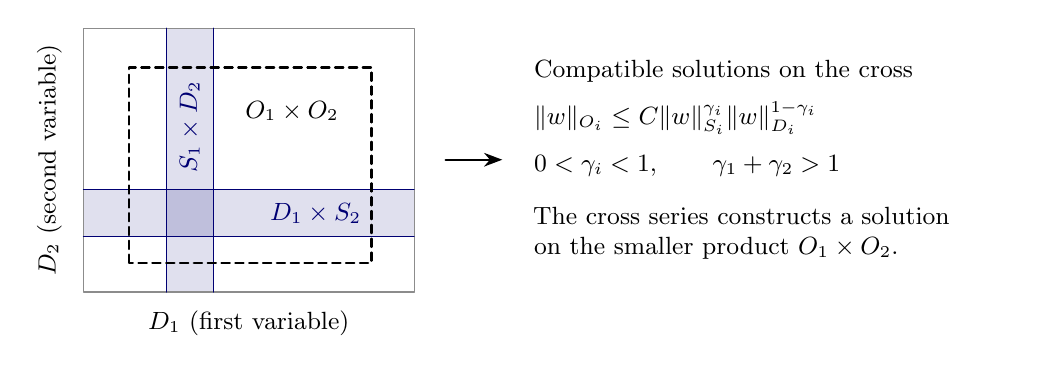
\begin{tikzpicture}[x=1cm,y=1cm,font=\small,>=Stealth,
  line cap=round,line join=round]
  \colorlet{crossink}{blue!45!black}
  \fill[crossink!12] (0,0.70) rectangle (4.2,1.30);
  \fill[crossink!12] (1.05,0) rectangle (1.65,3.35);
  \fill[crossink!25] (1.05,0.70) rectangle (1.65,1.30);
  \draw[black!45] (0,0) rectangle (4.2,3.35);
  \draw[crossink,thin] (0,0.70)--(4.2,0.70)
    (0,1.30)--(4.2,1.30) (1.05,0)--(1.05,3.35)
    (1.65,0)--(1.65,3.35);
  \draw[densely dashed,thick] (0.58,0.37) rectangle (3.66,2.85);
  \node[fill=white,inner sep=3pt] at (2.65,2.30) {$O_1\times O_2$};
  \node[text=crossink] at (2.95,1.00) {$D_1\times S_2$};
  \node[text=crossink,rotate=90] at (1.35,2.10) {$S_1\times D_2$};
  \node[anchor=north] at (2.10,-0.12) {$D_1$ (first variable)};
  \node[rotate=90,anchor=south] at (-0.15,1.68) {$D_2$ (second variable)};
  \draw[->,thick] (4.60,1.68)--(5.32,1.68);
  \node[anchor=west,align=left,text width=6.10cm] at (5.60,1.68) {
    Compatible solutions on the cross\\[6pt]
    $\displaystyle
       \|w\|_{O_i}\leq C\|w\|_{S_i}^{\gamma_i}
                              \|w\|_{D_i}^{1-\gamma_i}$\\[6pt]
    $\displaystyle 0<\gamma_i<1,\qquad \gamma_1+\gamma_2>1$\\[8pt]
    The cross series constructs a solution\\
    on the smaller product $O_1\times O_2$.
  };
\end{tikzpicture}


 \caption{Compatible product solutions are given on the shaded cross.
 The $L^2$ interpolation estimates for single-variable solutions,
 with $\gamma_1+\gamma_2>1$, make the
 singular-function series converge on $O_1\times O_2$.
 The drawing is schematic: each factor is a multidimensional domain,
 and containment of $S_i$ in $O_i$ is not required.}
 \label{cross:figure}
\end{figure}

\subsection{A geometric criterion for local extension}

We next build the interpolation estimates needed in
Lemma~\ref{cross:series}.  For a metric $g$, call a smooth real function
$\theta$ a \emph{strict weight} at a point where $\dd\theta\ne0$ if
\begin{equation}\label{cross:strict-weight}
 \operatorname{Hess}_g\theta(e,e)
  +\operatorname{Hess}_g\theta(v,v)>0
 \quad\text{for all }v\perp e,\ |v|_g=1,
 \qquad e=\frac{\nabla^g\theta}{|\nabla^g\theta|_g}.
\end{equation}
The strict scalar Carleman estimate gives, after shrinking the
coordinate neighborhood,
\begin{equation}\label{cross:carleman}
 \tau^3\|e^{\tau\theta}w\|_{L^2}^2
 +\tau\|\nabla(e^{\tau\theta}w)\|_{L^2}^2
 \le C\|e^{\tau\theta}Lw\|_{L^2}^2,
 \qquad \tau\ge\tau_0,
\end{equation}
for compactly supported $w$.
This is the elliptic strict-weight estimate of the classical
Carleman theory; see \citet[Chapter~XXVIII]{HormanderIV2009} and
\citet[Definition~8.3 and Theorem~9(a)]{KochTataru2005}.
Here the hypotheses can also be checked directly.  For $L=-\Delta_g$,
write $v=e^{\tau\theta}w$ and
\[
 e^{\tau\theta}Le^{-\tau\theta}=A_\tau+B_\tau,\qquad
 A_\tau=-\Delta_g-\tau^2|\dd\theta|_g^2,\quad
 B_\tau=\tau(2\nabla^g\theta\cdot\nabla+\Delta_g\theta).
\]
Here $A_\tau$ is self-adjoint and $B_\tau$ is skew-adjoint for
metric volume.  Integration by parts gives
\begin{align*}
 \|(A_\tau+B_\tau)v\|^2
 &=\|A_\tau v\|^2+\|B_\tau v\|^2
       +([A_\tau,B_\tau]v,v),\\
 ([A_\tau,B_\tau]v,v)
 &=4\tau\int\operatorname{Hess}_g\theta(\nabla v,\nabla\overline v)
   +4\tau^3\int\operatorname{Hess}_g\theta
                 (\nabla\theta,\nabla\theta)|v|^2
   -\tau\int(\Delta_g^2\theta)|v|^2.
\end{align*}
Choose a real constant $m$ strictly between the negative of the least
unit tangential Hessian value and the unit normal Hessian value.
After shrinking the patch, these inequalities have a positive margin.
Add $4m\tau(A_\tau v,v)$ to the commutator form.  Its gradient
coefficient becomes $4\tau(\operatorname{Hess}_g\theta+mg)$,
and its leading zero-order coefficient is
\[
 4\tau^3|\dd\theta|_g^2
       \big(\operatorname{Hess}_g\theta(e,e)-m\big)>c\tau^3.
\]
The tangential gradient form is positive.  Its mixed and possibly
negative normal terms cost at most
$C\tau\|\nabla_e v\|^2$, and
\[
 \|\nabla_e v\|^2
 \le C\tau^{-2}\|B_\tau v\|^2+C\|v\|^2.
\]
Finally
$|4m\tau(A_\tau v,v)|\le\tfrac12\|A_\tau v\|^2+
C\tau^2\|v\|^2$.
For large $\tau$, the squared parts absorb the normal derivative
cost and the positive zero-order term absorbs the remaining errors.
This yields \eqref{cross:carleman}.  Smooth first- and zero-order terms
in $L$ cost only $C(\|\nabla v\|^2+\tau^2\|v\|^2)$ and are absorbed
in the same way.  The proof gives uniform constants on fixed compact
sets of strict weights and bounded coefficients.

The existence criterion is a condition on a hypersurface in the
product.  Hessians in the following statement use the product
connection of $g_1$ and $g_2$.

\begin{proposition}[Product extension criterion]\label{cross:criterion}
Let $\rho$ be smooth near $z_0=(x_0,y_0)$, with $\rho(z_0)=0$ and
$\dd_x\rho,\dd_y\rho\ne0$.  Put
\[
 a_i=\frac{\nabla_i\rho}{|\nabla_i\rho|^2},\qquad H=\operatorname{Hess}\rho.
\]
Suppose that at $z_0$
\begin{equation}\label{cross:hessian-test}
 H((a_1,-a_2),(a_1,-a_2))
 +H((v_1,v_2),(v_1,v_2))>0
 \quad
 \left(v_i\perp a_i,\ |v_i|=|a_i|\right).
\end{equation}
Every product solution given on $\{\rho>0\}$ near $z_0$ extends to
a neighborhood of $z_0$, agreeing on a smaller part of that side.
In fact, the construction uses only two compact product sets in
$\{\rho>\epsilon\}$ for some $\epsilon>0$.
The neighborhoods and estimates on smaller neighborhoods are uniform
under small smooth perturbations preserving the strict hypotheses,
provided the data on those compact sets are bounded.
\end{proposition}

\begin{proof}
We first split the product Hessian condition into a strict weight in
each factor. Their sum will lie below a defining function for the given
side, with a quadratic gap. That gap places two intersecting product
sets in the given side; the weights then yield interpolation exponents
greater than one half, allowing Lemma~\ref{cross:series} to apply.

\paragraph{Splitting the weight between the factors.}
We seek symmetric forms $P_i$ satisfying
\[
 P_i(a_i,a_i)+P_i(v_i,v_i)>0,
 \qquad H+K\,\dd\rho^{\otimes2}>P_1\oplus P_2
\]
for some $K>0$, with the vectors $v_i$ as in
\eqref{cross:hessian-test}. After division by $|a_i|^2$, the first
inequality is the strict-weight condition for a function with gradient
$\nabla_i\rho$ and Hessian $P_i$. The second inequality will give the
quadratic gap. To obtain these forms by convex separation, the dual
tests are positive semidefinite forms $D$ whose diagonal blocks are
\[
 d_i a_i^{\otimes2}+S_i,\qquad
 d_i\ge0,\quad S_i\ge0\text{ on }a_i^\perp,
 \quad \tr S_i=d_i|a_i|^2.
\]
This follows by separating the open convex cone consisting of positive
definite forms plus the allowed $P_1\oplus P_2$; the individual dual
cones are generated by $a_i^{\otimes2}+v_i^{\otimes2}$.
Normalize $\tr D=1$.  To obtain a suitable $K$, it suffices by
compactness to prove $H:D>0$ on tests with $D\,\dd\rho=0$.

Represent such a $D$ as a covariance matrix.  The normal components
measured by the two partial covectors are opposite.  The diagonal-block
condition makes each normal component uncorrelated with its own
tangential component, hence with both tangential components.
Their variances coincide, giving $d_1=d_2=d>0$ and
\[
 D=d(a_1,-a_2)^{\otimes2}+D_\perp,
 \qquad \tr(D_\perp)_{ii}=d|a_i|^2.
\]
The case $d=0$ would force $D=0$.  Among nonnegative tangential forms
with these two fixed traces, every extreme point has rank one:
on an image of rank $r\ge2$, a nonzero symmetric perturbation preserves
the two traces because $r(r+1)/2>2$, and small perturbations of both
signs preserve positivity.  The rank-one tests are precisely those
in \eqref{cross:hessian-test}, multiplied by $d$.
The asserted positivity follows.  Compactness of the normalized tests
then supplies $K$, as required.

Prescribe gradients $\dd_i\rho$ and Hessians $P_i$ for smooth functions
$\theta_i$ vanishing at the respective points.  In small coordinates
centered there, Taylor expansion gives
\begin{equation}\label{cross:quadratic-gap}
 \theta_1(x)+\theta_2(y)
 \le \widetilde\rho(x,y)-c(|x|^2+|y|^2),
 \qquad \widetilde\rho=\rho+K\rho^2/2,
\end{equation}
with $c>0$.  Each $\theta_i$ satisfies
\eqref{cross:strict-weight}.  The positive side of $\widetilde\rho$
is the positive side of $\rho$ in this neighborhood.

\paragraph{Placing the cross and obtaining interpolation.}
Use coordinates $(s_i,z_i)$ with $s_i=\theta_i$. Fix a small
$\kappa>0$ so that $\phi(s_i)=s_i-\kappa s_i^2$ remains a strict weight.
Choose successively a small lateral radius $R$, a height
$l\ll cR^2$, and $e\ll\kappa l^2$.  Take
\[
 D_i=\{-l<s_i<l+4e,\ |z_i|<R\}.
\]
Use a cutoff equal to one on the inner lateral half and for
$-l+3e<s_i<l+2e$, supported in the cylinder and in
$-l+2e<s_i<l+3e$.
Let $S_i\Subset D_i$ include neighborhoods of its top and lateral
derivative supports, where respectively
\[
 s_i>l+e/2\quad\text{or}\quad |z_i|>R/3,
\]
and an inner top slice near $s_i=l+5e/4$.
The two closed product sets $\overline{D_1\times S_2}$ and
$\overline{S_1\times D_2}$ lie strictly in the given side.
For a top slice, the sum of the two $s$ coordinates is positive.
For a lateral slice, it is greater than $-2l$, which is dominated
by the quadratic gap in \eqref{cross:quadratic-gap}.
Making the sets slightly smaller if necessary gives a common
$\epsilon>0$ with $\rho>\epsilon$ on their closures.

For an $L_i$-solution normalized by $\|w\|_{L^2(D_i)}=1$, apply
\eqref{cross:carleman} to this cutoff times $w$.  Interior estimates
bound the bottom derivative terms using the large norm and the weight
$\phi(-l+3e)$.  The remaining derivative terms use
$\|w\|_{L^2(S_i)}$ and a weight at most $\phi(l+3e)$.
On a smaller inner cylinder beginning at $s_i=-e$, the weight is at
least $\phi(-e)$.  Balancing the two exponentials yields
\eqref{cross:interpolation-input} with
\begin{equation}\label{cross:exponent}
 \gamma_i=
 \frac{\phi(-e)-\phi(-l+3e)}{
       \phi(l+3e)-\phi(-l+3e)}>\frac12.
\end{equation}
Indeed at $e=0$ the quotient is $1/2+\kappa l/2$.
Values of the balancing parameter below $\tau_0$ are covered by
increasing the constant.  The output cylinder may be chosen to include
a connected tube from the origin to the indicated top slice.

\paragraph{Constructing and identifying the extension.}
Lemma~\ref{cross:series} now gives a product solution on a neighborhood
of $z_0$. It agrees with the old solution there on the positive side:
from a sufficiently near positive-side point, increase $s_2$ into
the top slice.  Since $\partial_{s_2}\rho>0$ locally, the segment stays
on that side and in the larger constructed cylinder.  Agreement on
the slice and unique continuation along a neighborhood of the segment
prove agreement at the original point.
All choices have strict margins.  Keeping their finitely many compact
sets and shrinking their output neighborhoods once proves the stated
perturbation uniformity by \eqref{cross:carleman},
Lemma~\ref{cross:series} and interior elliptic estimates.
\end{proof}

\subsection{Gluing along a compact family of surfaces}

Proposition~\ref{cross:criterion} provides a germ across one surface
point.  The following formulation records the geometry needed to
combine these germs.  In particular, agreement is proved on specified
overlap components, rather than inferred from the existence of a cover.

\begin{lemma}[Propagation through a compact cylinder]
\label{cross:propagation}
Suppose a region in a product patch has smooth coordinates $(z,a)$
near $B\times[a_-,a_+]$, where $B$ is a compact base, possibly with
boundary or corners.  A product solution is given on a neighborhood
of the top and lateral boundary and on an open set $\mathcal S$.
Assume that $\mathcal S$ is upward closed in $a$ at fixed $z$ and
contains these boundary neighborhoods.  If every level $a=\text{constant}$
satisfies Proposition~\ref{cross:criterion} outside $\mathcal S$, with
the positive side pointing toward increasing $a$, the solution extends
to a neighborhood of the cylinder, agreeing on $\mathcal S$.
For fixed coordinates, compact sets and strict reference inequalities,
the extension has uniform compact-subset bounds under small smooth
perturbations, in terms of bounds on finitely many compact subsets of
the initially given region.
\end{lemma}

\begin{proof}
Starting from the top, let $a_*$ be the infimum of levels down to which
an extension agreeing with the seed has been obtained.  In the uniform
version include uniform bounds in this property.  At a non-seed point
of $B\times\{a_*\}$, Proposition~\ref{cross:criterion} uses compact
data strictly above that level.  Take a finite cover of the level by
such output neighborhoods and seed neighborhoods.  Their data are
contained above $a_*+\eta$ for one $\eta>0$, so an already reached
level supplies them with the needed bounds.

Shrink the outputs in $(z,a)$ coordinates to boxes
$B_i\times(a_*-d_i,a_*+d_i)$.
Every connected component of an overlap contains vertical segments
to a common height greater than $a_*$.  Both germs equal the preceding
extension there.  Unique continuation for $L_1^x+L_2^y$ makes them
identical on that overlap component.  The same argument gives agreement
with $\mathcal S$, because a vertical segment moving upward from a
seed point stays in the seed.  Boundary neighborhoods use the given
solution.  A finite subcover has a positive minimum output width and
therefore passes the putative last level, or includes the endpoint
$a_-$.  This proves continuation on the whole cylinder.
The same finite constructions retain all strict margins under small
perturbations.  Their Carleman, series and interior estimates prove
the uniform assertion.  Data bounded up to a limiting surface are
never required: each local construction uses compact sets strictly
above it.
\end{proof}

\subsection{Initialization at a fixed distance from the diagonal}

We apply the criterion to a mixed Green kernel.  Let $g_1,g_2$ be smooth
metrics in coordinate patches centered at $0$, obtained from interior
patches of compact Dirichlet manifolds.  Suppose they agree on an open
set $W$ containing the lower side of a smooth hypersurface through $0$.
After a linear coordinate change, assume
\[
 g_1(0)=g_2(0)=I,\qquad
 \{x_n<q(x')\}\subset W\text{ near }0,\qquad
 q(0)=0,\quad \dd q(0)=0,
\]
for a smooth function $q$.  No regularity of the rest of $\partial W$
is assumed.
Let $G_j$ be the Dirichlet Green kernels, normalized with metric volume,
and suppose $G_1=G_2$ on $W\times W$.
For a small dilation parameter $\lambda>0$, put
\begin{equation}\label{cross:dilation}
 g_{j,\lambda}(z)=g_j(\lambda z),\qquad
 G_{j,\lambda}(x,y)=\lambda^{n-2}G_j(\lambda x,\lambda y),
 \qquad W_\lambda=\lambda^{-1}W.
\end{equation}
On each fixed bounded patch the metrics tend smoothly to the Euclidean
metric, and $W_\lambda$ contains every fixed compact subset of
$\{z_n<0\}$ for sufficiently small $\lambda$.
Initially define, off the diagonal,
\begin{equation}\label{cross:mixed-data}
 \mathcal G_\lambda(x,y)=
 \begin{cases}
 G_{1,\lambda}(x,y),&y\in W_\lambda,\\
 G_{2,\lambda}(x,y),&x\in W_\lambda.
 \end{cases}
\end{equation}
The pieces fit and solve the first equation in $x$ and the second in $y$.

\begin{proposition}[Fixed-separation initialization]\label{cross:initial}
In this setting, let $n\ge3$ and fix $B>0$, $d>0$ and $\eta>0$.
For all sufficiently small $\lambda$, the data
\eqref{cross:mixed-data} have a product-solution continuation to a
neighborhood of
\[
 \{(x,y):|x|,|y|\le B,\ |x-y|\ge d\}.
\]
Every fixed $C^m$ norm on a smaller neighborhood is bounded uniformly
in $\lambda$.  The continuation agrees with $G_{1,\lambda}$ where
$y_n<-\eta$ and with $G_{2,\lambda}$ where $x_n<-\eta$, on the
corresponding overlaps.  The smallness threshold for $\lambda$ and
the constants may depend on $B,d,\eta,m$.
\end{proposition}

\begin{proof}
We first cross the limiting plane, then deform variable-radius tubes
to reach the prescribed separations.  All the sets and positive
separation margins used in the two steps are fixed before choosing
$\lambda$.

\paragraph{Crossing the plane and obtaining a common seed.}
We first extend slightly across the plane in one variable while keeping
the other at a comparable positive separation. The first interpolation
exponent can be made close to one; this compensates for the fixed
positive exponent obtained by propagation in the separated second
variable.

Fix a point $x_0$ of height zero and a separation scale $s>0$.
In the second factor take
\[
 D_2=\{s/2<|y-x_0|<2s\}
\]
and an observed ball $S_2$ about $x_0-se_n$.
In the first take a ball of radius $3\tau_0s$ centered at
$x_0-\tau_0se_n$, with $\tau_0>0$ fixed small enough that the two
large domains are separated.  Its observed ball has radius
$(1-\alpha)\tau_0s$, with $\alpha>0$ to be chosen.
These observed balls lie strictly in the lower half-space.

There is a two-constants estimate from $S_2$ to a slightly enlarged
closed annulus $4s/5\le|y-x_0|\le6s/5$, with an exponent
$\gamma_2>0$ independent of $\alpha$.  Here is a direct way to obtain
it with room for perturbations.  On a Euclidean annulus the weight
$|z-z_*|^{-1}$ is strict: its radial Hessian is
$2|z-z_*|^{-3}$ and each tangential Hessian value is
$-|z-z_*|^{-3}$.  Radial cutoffs in
\eqref{cross:carleman}, followed by exponential balancing, propagate
smallness from an inner ball to an intermediate ball using the norm
on an outer ball.  A finite chain of overlapping balls with enlarged
balls inside $D_2$ connects $S_2$ to the target annulus.  The annulus
is connected since $n\ge3$.  Multiplying the finitely many positive
exponents gives the asserted $\gamma_2$.  The same weights and margins
work for sufficiently small perturbations of the Euclidean metric.

In the first factor use this radial argument centered at
$x_0-\tau_0se_n$.  Keep the outer cutoff a fixed distance beyond radius
$\tau_0s$, and put the inner cutoff just inside radius
$(1-\alpha)\tau_0s$.  Take a concentric target ball of radius
$(\tau_0+c)s$, with $c>0$ small; it contains the observed ball and
a ball of radius $cs$ about $x_0$.
As $\alpha$ and $c$ decrease, the target weight approaches the inner weight.
The interpolation exponent therefore tends to one.  Choose these
constants so that $\gamma_1+\gamma_2>1$.
Lemma~\ref{cross:series} extends the kernel to a small ball about
$x_0$ times the target annulus.  On these fixed separated sets the
rescaled Green kernels and their derivatives are uniformly bounded:
the local Green singularity is $O(|x-y|^{2-n})$, and interior elliptic
estimates give derivative bounds away from the pole.

The extensions agree with both lower pieces.  Agreement for $y\in S_2$
comes from the first expansion.  For fixed $x$ below a sufficiently
small negative height, continue in $y$ through the connected target
annulus to compare with $G_{2,\lambda}$.  For a second point below that
height, compare with $G_{1,\lambda}$ by continuation in the first
variable from its observed ball.  All comparisons remain separated.

The local extensions must next be compared on overlaps. Retain much
smaller first balls and narrower annuli for coverage, keeping the larger
products as comparison domains. The unused margins allow both variables
to move into the known lower region. Overlapping retained products have
scales comparable to $|x-y|$. For two products of the same orientation,
lower their near-plane variable into the known region; the path stays
inside both larger first balls.  For products of opposite orientations,
both variables lie in retained near-plane balls. On the fixed compact
range of locations and positive separation scales, choose the retained
products with strict ball and annular margins, then take $\eta_0>0$
much smaller than the smallest retained width. Lower both variables by
\[
 h=\max(x_n,y_n,0)+2\eta_0.
\]
By making the retained balls a sufficiently small fraction of the larger
balls, the path stays in both larger products: its displacement is
smaller than their ball and annular margins. Its endpoint has both
heights below $-\eta_0$,
where both germs are the original kernel.  Unique continuation along
a neighborhood of the path proves agreement.  Choose
$\eta_0\le\eta$ and then $\lambda$ small enough for this truncated
lower half-space to lie in $W_\lambda$ on all sets used.

Interchanging the two variables and covering gives, for some fixed
$c_0>0$, a single-valued continuation in
\begin{equation}\label{cross:coarse-region}
 \min(x_n,y_n)<c_0|x-y|,
\end{equation}
on every fixed compact range of bounded locations and positive
separations.  The estimates are uniform in $\lambda$ on that range.
For coverage near the plane, take $x_0=(x',0)$ and
$s=|y-x_0|$ when the first variable has the smaller nonnegative height;
then $x$ is in the retained first ball and $y$ in the retained annulus
if $c_0$ is small.  Points already below the plane are covered by the
same construction near it or by the given cross farther below it.
The preceding overlap argument makes these choices compatible.

\paragraph{Sweeping tubes inward from the common seed.}
The region \eqref{cross:coarse-region} is now the seed for the second
stage. At fixed center $y$ and direction $\omega$, we move $x$ along the
ray from $y$: large radii lie in the seed, and decreasing the radius
will reach the target pairs. Choose $M>B+3$ and introduce
\begin{equation}\label{cross:tubes}
 t=M+y_n+e_0|y'|^2,\qquad r_a(y)=a t^{1+\sigma},\qquad
 x=y+r_a(y)\omega,\quad |\omega|=1,
\end{equation}
where $\sigma,e_0>0$ will be small.  The base is
\[
 y_n\ge-B-1,\qquad t\le T_0,\qquad \omega\in\mathbb S^{n-1},
\]
and $a$ decreases through a fixed interval $[a_{\min},a_{\max}]$.
The term $e_0|y'|^2$ makes this base compact. The parameter $a$ decreases
while $(y,\omega)$ remains fixed, as required by the compact-cylinder
propagation lemma.
Take $a_{\min}$ small enough that the target separations exceed
$r_{a_{\min}}(y)$, and $a_{\max}$ large enough that its whole level
satisfies \eqref{cross:coarse-region}.  The bottom base boundary has
$y_n<0$.  Take $T_0$ so large that
$c_0a_{\min}T_0^\sigma>1$; its top boundary also satisfies
\eqref{cross:coarse-region}. Here the superlinear power $1+\sigma$
ensures that $r_a/t=a t^\sigma$ is large on this top face. Thus the
initial $a$-level and both base boundary faces are supplied by the seed.
This known region is upward closed in $a$: since
$\min(x_n,y_n)=y_n+r\min(\omega_n,0)$, its defining
inequality is $y_n<(c_0-\min(\omega_n,0))r$, whose radius coefficient
is positive.

It remains to check the strict extension criterion outside that region.
At the Euclidean metrics use
\[
 \rho=\tfrac12(|x-y|^2-r_a(y)^2),\qquad b=\nabla r_a.
\]
Away from $\omega+b=0$, multiply the vectors in
\eqref{cross:hessian-test} by the common positive factor $r_a$ and
write their real and imaginary parts as
\begin{equation}\label{cross:null-vectors}
 \begin{aligned}
 U_1&=\omega+iv,& |v|=1,\quad v\perp\omega,\\
 U_2&=\frac{\omega+b}{|\omega+b|^2}+iw,
 &w\perp(\omega+b),\quad |w|=|\omega+b|^{-1}.
 \end{aligned}
\end{equation}
The identity $\omega\cdot(U_1-U_2)=b\cdot U_2$ cancels the normal
part of the distance Hessian.  Consequently the test is
\begin{equation}\label{cross:tube-test}
 \big|\pi_{\omega^\perp}(U_1-U_2)\big|^2
 -(r_a\partial^2r_a)(U_2,\overline{U_2}).
\end{equation}
For bounded $b$, outside fixed small neighborhoods of
$b=-\omega$ and $b=-2\omega$, the first term is at least $c|b|^2$.
To see this, a zero forces the real part of $U_2$ to be parallel to
$\omega$, and equality of the projected imaginary lengths gives
$|\omega+b|=1$.  Thus $b=0$ or $b=-2\omega$.
Near $b=0$, the real projected difference controls
$|\pi_{\omega^\perp}b|$ to first order; also
\[
 |\pi_{\omega^\perp}w|
 =1-\omega\cdot b+O(|b|^2),
\]
so the imaginary projected difference controls $|\omega\cdot b|$
to first order.  This proves the quadratic lower bound near zero;
compactness proves it on the remaining range.

Outside \eqref{cross:coarse-region}, $y_n\ge c_0r_a$, so
$r_a/t\le1/c_0$ and
\[
 b=(1+\sigma)(r_a/t)\nabla t
\]
stays bounded.  When $\nabla t$ is close to $e_n$, the two excluded
neighborhoods already lie in \eqref{cross:coarse-region}.  Indeed,
\[
 \frac{x_n}{r_a}
 \le \frac{(1+\sigma)|\nabla t|}{|b|}+\omega_n,
\]
which is arbitrarily small near $b=-\omega$ and negative near
$b=-2\omega$ as $\sigma$ and the gradient error tend to zero.
On the complement $|U_2|$ is bounded and differentiation of
\eqref{cross:tubes} gives
\begin{equation}\label{cross:tube-error}
 r_a|\partial^2r_a|
 \le C(\sigma+T_0e_0)|b|^2.
\end{equation}
Choose the excluded-neighborhood sizes first in terms of $c_0$.
Use the positive lower bound on the remaining bounded $b$-range to
choose $\sigma$ small, then choose the $a$-interval and $T_0$ as above,
and finally $e_0>0$ so small that \eqref{cross:tube-error} is absorbed.
Choosing the transverse compactification last keeps its contribution
to the Hessian test small. These choices also make the gradient error small, since
$|\nabla t-e_n|\le2\sqrt{e_0T_0}$ on the base.
Thus \eqref{cross:tube-test} is strictly positive wherever continuation
is needed.  Both partial gradients are nonzero there.

All these sets are bounded and stay at separation at least
$a_{\min}(M-B-1)^{1+\sigma}>0$.  Smooth convergence of the metrics
therefore preserves the strict tests for sufficiently small $\lambda$.
Lemma~\ref{cross:propagation} continues the kernel through the cylinder,
with uniform estimates and agreement on the seed.  A target pair has
$a=|x-y|/t^{1+\sigma}\ge a_{\min}$; if $a>a_{\max}$ it is already in
the coarse region.  Hence every target pair is covered.

We also identify the extension with both pieces of the full cross
\eqref{cross:mixed-data}. Perform the construction with a larger bound
$B'>B$ and a smaller separation $0<d'<d$, chosen so that for every
$|y|\le B$ the domain
\[
 D_y=B(0,B')\setminus\overline{B(y,d')}
\]
is connected and contains a fixed lower open ball with $x_n<-\eta$.
Choose $B'$ large enough that every excluded closed ball lies strictly
inside $B(0,B')$ and is disjoint from that lower ball.
For fixed $y\in W_\lambda$ in the target range, the continuation
and $G_{1,\lambda}$ solve the same first-variable equation on $D_y$.
On the lower ball the continuation equals $G_{2,\lambda}$, which equals
$G_{1,\lambda}$ because both variables lie in $W_\lambda$.
Unique continuation on $D_y$ proves agreement on the required overlap.
Interchanging the variables proves agreement with the other piece.
Keeping slightly larger target bounds and a slightly smaller separation
before restricting to the prescribed range gives the claimed neighborhood
and its compact-subset estimates.
\end{proof}

The constants in Proposition~\ref{cross:initial} may deteriorate as
$d\downarrow0$.  Its role is to initialize a construction at finitely
many fixed positive scales.  Lemma~\ref{cross:propagation} will also
provide qualitative existence at each positive radius in a shrinking
family; the uniform estimate for that family is established below.
% END work/intake-assessment/manuscript/Smooth-Anisotropic-Uniqueness-in-the-Calderon-Problem-from-One-Boundary-Patch-September-24-2026/build/sections/03-product-continuation.tex

% BEGIN work/intake-assessment/manuscript/Smooth-Anisotropic-Uniqueness-in-the-Calderon-Problem-from-One-Boundary-Patch-September-24-2026/build/sections/04-shrinking-balls.tex
\section{Continuation to shrinking spheres}\label{sec:balls}

We now apply the product continuation criterion near a point where an
isometry is already known on one side.  The purpose of this section is to
construct a family of functionals on harmonic functions, represented on
small spheres.  Their existence will follow from the geometry of the
spheres.  A uniform bound for the functionals, needed when the spheres
shrink, will follow from the estimate in the next section.

\subsection{The local data and their normalization}
\label{balls:setup}

Throughout Sections~\ref{sec:balls}--\ref{sec:bootstrap}, fix the
manifolds $(N_j,g_j)$, actual Dirichlet Green functions $G_j$, common
harmonic coordinate neighborhood $\Omega$, matching set $W$, and finite
harmonic pairs $(u_1^a,u_2^a)$ of Theorem~\ref{local:extension}.
Thus the coordinate metrics and paired functions agree on $W$, and the
Green kernels agree on $W\times W$ off the diagonal. The first-side
coordinate Hessians span the hyperplane annihilated by $g_1^{-1}(0)$. An interior ball in
$W$ tangent at $0$ supplies the one-sided hypersurface required by
that theorem. We construct the sphere functionals for these data.

A linear change of harmonic coordinates makes $g_1(0)=g_2(0)=I$ and
writes the separating hypersurface as a graph tangent to $x_n=0$, with
the known side below it.  For a spatial
dilation $\lambda>0$, write
\begin{equation}\label{balls:dilation}
 g_{j,\lambda}(x)=g_j(\lambda x),\qquad
 G_{j,\lambda}(x,y)=\lambda^{n-2}G_j(\lambda x,\lambda y).
\end{equation}
Dilate the harmonic pairs at the same time:
\[
 u_{j,\lambda}^a(x)=u_j^a(\lambda x).
\]
They remain harmonic for $g_{j,\lambda}$ and agree on the dilated known
set. The metrics and Green kernels in \eqref{balls:dilation} have the
corresponding normalization on the dilated neighborhoods. On each fixed
bounded coordinate set the metrics converge smoothly to $I$ as $\lambda\downarrow0$.  The dilated known set
contains every fixed compact set lying strictly below $x_n=0$, once
$\lambda$ is sufficiently small.

Use $x$ for the first variable and $y$ for the second.  The mixed kernel
$\mathcal G$ is initially $G_{1,\lambda}$ when $y$ is in the known set,
and $G_{2,\lambda}$ when $x$ is in that set.  These prescriptions agree on
their overlap and solve the first equation in $x$ and the second in $y$,
away from the diagonal.  Proposition~\ref{cross:initial} continues this
kernel to any specified compact region of fixed positive separation,
with smooth bounds uniform for small $\lambda$.  We shall use that result
only after all the positive separation ranges in question have been fixed.

The geometry of a moving sphere dictates the next choices. In the
strict extension test, the leading terms involving the gradient of its
radius cancel; strict concavity of the logarithmic radius supplies the
remaining positive term (see \eqref{balls:test-expression}). We therefore
choose a conformal reference metric for which a depth function is
strictly concave. Separately, a scalar normalization of the second
inverse metric will give the two inverse matrices the same trace
relative to the reference metric. The harmonic Hessians will determine
their remaining difference.

Fix the coordinate cylinder
\[
 Y=\{y=(y',y_n): |y'|\leq1,\ -1\leq y_n\leq1\},
 \qquad t_0(y)=y_n+|y'|^2.
\]
Take a sufficiently large fixed number $L$ and put
\begin{equation}\label{balls:normalization}
 \gamma=e^{-2Lt_0}g_{1,\lambda},\qquad
 Q=\frac{n\,g_{2,\lambda}^{-1}}
          {\operatorname{tr}(\gamma g_{2,\lambda}^{-1})},\qquad
 h=Q-\gamma^{-1}.
\end{equation}
Thus $Q$ is the principal matrix of a positive multiple of the second
equation and $\operatorname{tr}(\gamma h)=0$.  The first equation can
likewise be multiplied by a positive function to give principal metric
$\gamma$.  Such multiplication does not change its solutions.  The
metric $\gamma$ will also identify the two tangent spaces at a common
coordinate point.  All these coefficients have uniform smooth bounds
on a fixed neighborhood of $Y$ for sufficiently small $\lambda$, and
$h\to0$ in every fixed smooth norm as $\lambda\downarrow0$.

Define the depth function
\begin{equation}\label{balls:depth}
 t(y)=\int_{1/8}^{t_0(y)}e^{-2Ls}\,ds.
\end{equation}
It is negative at $0$ and has nonvanishing differential on $Y$.  The
conformal connection formula gives
\begin{equation}\label{balls:depth-hessian}
 \operatorname{Hess}_{\gamma}t
 =e^{-2Lt_0}\bigl(
    \operatorname{Hess}_{g_{1,\lambda}}t_0
       -L|dt_0|_{g_{1,\lambda}}^2g_{1,\lambda}\bigr)
 \leq-c\gamma.
\end{equation}
Indeed $|dt_0|$ is bounded below, whereas the first Hessian on the right is
uniformly bounded.  Choose $L$ first and then an upper bound for
$\lambda$ so that the displayed strict inequality holds with fixed $c>0$.

\subsection{Radii and cutoff regions}

For a fixed integer $p\geq2$, a positive amplitude $R_*$, and
$0<\delta\leq1$, define
\begin{equation}\label{balls:radius}
 \ell_\delta(t)=\delta\log(1+e^{t/\delta}),\qquad
 r_\delta(y)=R_*\ell_\delta(t(y))^p,
 \qquad f_\delta=\log r_\delta,\quad
 \beta_\delta=|df_\delta|_\gamma.
\end{equation}
The balls will be the $\gamma$-geodesic balls with center $y$ and radius
$r_\delta(y)$, lying in the first coordinate neighborhood. As the lemma
below shows, they collapse where $t\le0$, including a neighborhood of
the contact point, but their radii stay bounded below where $t$ is
bounded away from zero on the positive side. This distinction will keep
cutoff derivatives away from uncontrolled shrinking spheres.

\begin{lemma}[Profile bounds]\label{balls:profiles}
On $Y$, after the preceding choices of geometry, the following bounds
hold uniformly for small $\lambda$, $0<\delta\leq1$, and $p\geq2$:
\begin{equation}\label{balls:profile-estimates}
 \beta_\delta\geq c p,\qquad
 \operatorname{Hess}_\gamma f_\delta\leq-c\beta_\delta\gamma,
 \qquad |\partial^j f_\delta|\leq C_j\beta_\delta^j
 \quad(j\geq1).
\end{equation}
The constants $c,C_j$ do not depend on $p$.  The functions
$r_\delta^{1/p}$ have a Lipschitz bound independent of $\delta$ and
$\lambda$ for fixed $p,R_*$.  The radii increase with $\delta$, tend to
zero on $\{t\leq0\}$ as $\delta\downarrow0$, and satisfy
\begin{equation}\label{balls:radius-smallness}
 \sup_{\delta,y}r_\delta\beta_\delta^2\longrightarrow0
 \quad\text{as }R_*\downarrow0
\end{equation}
for each fixed $p$.
\end{lemma}

\begin{proof}
Write $a_\delta=(\log\ell_\delta)'$.  In terms of $s=t/\delta$,
\[
 a_\delta(t)=\delta^{-1}A(s),\qquad
 A(s)=\frac{e^s}{(1+e^s)\log(1+e^s)}.
\]
The function $A$ is positive and decreasing.  At the negative end it
tends to one, and at the positive end it is comparable to $(1+s)^{-1}$.
Differentiating the formula, or its convergent expressions at the two
ends, gives $|A^{(j)}(s)|\leq C_jA(s)^{j+1}$.  On the remaining compact
interval the same inequalities follow by positivity.  On the fixed
$t$ interval this gives a positive lower bound for $a_\delta$ and
\[
 a_\delta'\leq0,\qquad
 |\partial_t^j\log\ell_\delta|\leq C_j a_\delta^j,
 \qquad a_\delta\leq\ell_\delta^{-1}.
\]
Since $|dt|_\gamma$ is bounded above and below,
$\beta_\delta=p a_\delta|dt|_\gamma$.  Equation
\eqref{balls:depth-hessian} and
\[
 \operatorname{Hess}_\gamma f_\delta
   =p a_\delta\operatorname{Hess}_\gamma t
          +p a_\delta'\,dt\otimes dt
\]
prove the Hessian bound.  The chain rule proves the other derivative
bounds, with constants independent of $p\geq2$ because
$p a_\delta^j\leq p^j a_\delta^j$.

The bound $0<\ell_\delta'<1$ gives the asserted Lipschitz estimate for
$r_\delta^{1/p}=R_*^{1/p}\ell_\delta\circ t$.  Moreover,
\[
 \partial_\delta\ell_\delta
  =\log(1+e^s)-\frac{s e^s}{1+e^s}>0.
\]
The function on the right increases up to $s=0$ and decreases afterward,
with limit zero at both ends.  The pointwise limit of $\ell_\delta$ is
$\max(t,0)$.  Finally,
\[
 r_\delta\beta_\delta^2
       \leq C R_*p^2\ell_\delta^{p-2},
\]
and $\ell_\delta$ is uniformly bounded on the fixed interval.  This
proves \eqref{balls:radius-smallness}.
\end{proof}

Choose $t_b>0$ so small that $3t_b<t(1/4)$, where on the right $t$ denotes
the increasing function of $t_0$ in \eqref{balls:depth}, and set
\begin{equation}\label{balls:K}
 K=\{y\in Y:y_n\geq-1/2,\ t(y)\leq2t_b\}.
\end{equation}
Then $K\Subset Y^\circ$.  We fix a smooth cutoff $\chi\in
C_c^\infty(Y^\circ)$ equal to one on a neighborhood of $K$, with
\begin{equation}\label{balls:cutoff-region}
 \operatorname{supp}(d\chi)\subset
       \{y_n<-1/4\}\cup\{t>t_b\}.
\end{equation}
For example, multiply a cutoff that changes from zero to one between
$y_n=-3/4$ and $y_n=-1/2$ by a cutoff of $t$ that changes from one to zero
between $2t_b$ and $3t_b$, moving the endpoints slightly to make it one
on a neighborhood of $K$.  The inequality $3t_b<t(1/4)$ keeps its support
away from the lateral and upper faces of $Y$.  This gives fixed room
around $K$ and places every cutoff derivative either in the known lower
region or where
\[
 r_\delta\ge R_*t_b^p>0.
\]
Thus the later estimates for the sphere functionals can use the original
Green kernel or fixed-separation continuation on every cutoff derivative
support.

\subsection{The strict test at a moving sphere}

For coordinate derivatives of the tensor $h$, use the pointwise notation
\[
 H_8(y)=\sum_{|\alpha|\leq8}|\partial_y^\alpha h(y)|.
\]
We shall temporarily impose
\begin{equation}\label{balls:bootstrap-condition}
 H_8\leq\varepsilon r_\delta,\qquad
 r_{\delta'}\beta_{\delta'}^2\leq\varepsilon
       \quad(\delta\leq\delta'\leq1)
 \quad\text{on }Y.
\end{equation}
The first inequality measures how closely the two principal metrics
agree compared with the current radius.  It will be improved in
Section~\ref{sec:bootstrap}.

\begin{proposition}[Continuation to the sphere family]\label{balls:continuation}
Choose $p$ sufficiently large and then $\varepsilon>0$ sufficiently small
in terms of the fixed background bounds.  Choose $R_*>0$ small enough
that all the balls lie in normal neighborhoods and
\eqref{balls:radius-smallness} is at most $\varepsilon$.
For all sufficiently small spatial dilations $\lambda$, and every
$0<\delta\le1$ for which \eqref{balls:bootstrap-condition} holds, the mixed
kernel extends to a neighborhood of
\[
 \{(x,y):y\in Y,\ d_\gamma(x,y)=r_\delta(y)\}.
\]
The extension solves the two homogeneous equations and agrees with the
prescribed lower cross and the fixed-separation continuation.  It is
smooth for each positive $\delta$; no uniform norm as $\delta\downarrow0$
is asserted here.
\end{proposition}

\begin{proof}
We check Proposition~\ref{cross:criterion} at each intermediate radius
$r=r_{\delta'}$.  Put $f=\log r$, $\beta=|df|_\gamma$, and
$b=\nabla^\gamma r$, so $|b|=r\beta$.  Use the defining function
\[
 \rho(x,y)=\tfrac12\bigl(d_\gamma(x,y)^2-r(y)^2\bigr).
\]
The positive side is the outside of the sphere.  Parallel translation
along its radial geodesic identifies the two tangent spaces for
$\gamma$; write $\omega$ for the unit vector from $y$ to $x$.

In the normalization of the strict test, the normal and tangential
vectors can be combined into complex vectors
\[
 U_1=\omega+i v,\quad v\perp\omega,\quad |v|=1,
 \qquad U_2=q+i w,
\]
where the conditions for the second principal metric $Q^{-1}$ give
\begin{equation}\label{balls:test-vectors}
 (\omega+b)\cdot U_2=1,\qquad
 q=\frac{\omega+b}{|\omega+b|^2}+O(|h|),\qquad
 |w|=|\omega+b|^{-1}+O(|h|).
\end{equation}
Here and below lengths and dot products in these formulas use $\gamma$
and its parallel identification.  The first equation includes
$(\omega+b)\cdot w=0$.  Since $|b|$ and $|h|$ are small, both partial
gradients of $\rho$ are nonzero and $|U_2|$ is bounded above and below.

The Hessian of half the squared distance, with the product
$\gamma$-connection, evaluated on these endpoint vectors is
\[
 |U_1-U_2|^2+O(r^2)(|U_1|^2+|U_2|^2).
\]
To see the error size, parametrize the radial geodesic on $[0,1]$.
Its Jacobi field with prescribed endpoint values differs, in a parallel
frame, from the affine interpolant by $O(r^2)$ in $C^1$, by the Jacobi
equation and bounded curvature.  The second variation formula then gives
the displayed bound.  Replacing the second connection by that of
$Q^{-1}$ costs $O(r^2)$ as well: the connection difference is
$O(|h|+|\partial h|)=O(\varepsilon r)$ and $|d\rho|=O(r)$.

Now
$\omega\cdot(U_1-U_2)=b\cdot U_2$ and
$\operatorname{Hess}(r^2/2)=2\,dr\otimes dr+r^2\operatorname{Hess}f$.
Consequently the strict Hessian expression is
\begin{equation}\label{balls:test-expression}
 |\pi_{\omega^\perp}(U_1-U_2)|^2-|b\cdot U_2|^2
      -r^2\operatorname{Hess}_\gamma f(U_2,\overline U_2)+O(r^2).
\end{equation}
For a real Hessian, its value on a complex vector and its conjugate is
the sum of its values on the real and imaginary parts, as required by
the criterion.

The real part of the projected difference is
$-\pi_{\omega^\perp}b+O(|b|^2+|h|)$.  For its imaginary part,
\eqref{balls:test-vectors} gives
$|\pi_{\omega^\perp}w|=1-\omega\cdot b+O(|b|^2+|h|)$;
compare this with $|v|=1$.  Squaring these two bounds yields
\[
 |\pi_{\omega^\perp}(U_1-U_2)|^2
 \geq |b|^2-C\bigl(|b|^3+|b||h|+|h|^2\bigr).
\]
The real and imaginary directions of $U_2$ are almost orthonormal, so
\[
 |b\cdot U_2|^2\leq
       \bigl(1+C(|b|+|h|)\bigr)|b|^2.
\]
By Lemma~\ref{balls:profiles}, the expression
\eqref{balls:test-expression} is therefore bounded below by
\[
 c r^2\beta
  -C\bigl(r^2+r^3\beta^3+\varepsilon r^2\beta
                       +\varepsilon^2r^2\bigr).
\]
Choose $p$ so that $\inf\beta$ absorbs the $Cr^2$ term.  Then choose
$\varepsilon$ small.  The inequality $r\beta^2\leq\varepsilon$ absorbs
$r^3\beta^3$, and the expression is strictly positive.

It remains to specify the starting and boundary data for this local
test.  Deform $\delta'$ from $1$ to $\delta$, using $(y,\omega)$ as base
variables.  The inequality $H_8\leq\varepsilon r_\delta$ implies its
counterpart for every $\delta'\geq\delta$, because the radii increase
with $\delta'$.  At $\delta'=1$ the required separations have a fixed
positive minimum.  The same is true wherever $t>t_b$, since
$r_{\delta'}\geq R_*t_b^p$.  Proposition~\ref{cross:initial} supplies
uniformly bounded data on these fixed separation ranges, with open room.
Where $y_n<-1/4$, use the original $G_{1,\lambda}$; for small $\lambda$
this is part of the known lower cross.  These regions cover the lateral
and end boundaries of the cylinder that are not supplied by the initial
parameter, and their prescriptions agree on overlaps.

The base sphere bundle over the closed cylinder is compact.  On each
fixed interval $\delta\leq\delta'\leq1$, the radii are positive, all
surfaces lie in normal neighborhoods, and the strict tests just proved
apply away from the prescribed regions.  Lemma~\ref{cross:propagation}
therefore supplies compatible extension germs on the whole family.
Its finite-cover gluing also retains agreement with the prescribed
regions.  This is an existence argument for each finite interval; it
does not assert uniform continuation bounds when the lower endpoint
tends to zero.
\end{proof}

\subsection{Functionals represented on the spheres}

The mixed kernel now defines a map from first-metric harmonic functions
to second-metric harmonic functions.  Its representation on a small
sphere will allow us to estimate this map without estimating the kernel
through every continuation step.
Fix $0<\delta\le1$ and write $r=r_\delta$ in this subsection.

For a function $u$ harmonic for $g_{1,\lambda}$ near
$\overline{B_\gamma(y,r(y))}$, define
\begin{equation}\label{balls:flux}
 T_yu=\int_{\partial B_\gamma(y,r(y))}
  \bigl(\mathcal G(x,y)\partial_{\nu_1}u(x)
       -u(x)\partial_{\nu_1}\mathcal G(x,y)\bigr)\,dS_1(x).
\end{equation}
Here $\nu_1$ is the outer unit normal and $dS_1$ the hypersurface measure
for the actual first metric $g_{1,\lambda}$, not for $\gamma$.
Let $S_y$ be the unit sphere of $(T_y\mathbb R^n,\gamma_y)$, with its
rotation-invariant probability measure $d\sigma_y$.  Parametrize the
integration sphere by $x=\exp_y^\gamma(r(y)\omega)$.

\begin{proposition}[The transfer density]\label{balls:functional}
Under the assumptions of Proposition~\ref{balls:continuation}, there is
a smooth function $\psi(y,\omega)$ on the unit sphere bundle over
$Y^\circ$ such that
\begin{equation}\label{balls:density-representation}
 T_yu=\int_{S_y}\psi(y,\omega)
              u\bigl(\exp_y^\gamma(r(y)\omega)\bigr)\,d\sigma_y(\omega).
\end{equation}
For every fixed center $y_0$, if $u$ is first-metric harmonic on a
neighborhood of $\overline{B_\gamma(y_0,r(y_0))}$, then
$y\mapsto T_yu$ is defined and second-metric harmonic on a sufficiently
small neighborhood of $y_0$.  This neighborhood may depend on $u$.
In particular, for functions harmonic on the fixed coordinate
neighborhood required by the sphere family,
\begin{equation}\label{balls:reproduction}
 \int_{S_y}\psi\,d\sigma_y=1,
 \qquad T_yx^i=y^i,
 \qquad T_yu_{1,\lambda}^a=u_{2,\lambda}^a(y).
\end{equation}
On the support of derivatives of $\chi$, every fixed angular smooth
norm of $\psi$ and its first base derivatives is bounded independently
of $\delta$ and small $\lambda$, after $p,R_*$ and the fixed geometry
have been chosen.
\end{proposition}

\begin{proof}
For each ball, its smooth Dirichlet solution operator determines the
normal derivative of a harmonic function from its boundary trace.
Move this boundary operator in the first term of \eqref{balls:flux}
onto the smooth boundary value of $\mathcal G$ by adjunction, and then
pull back to $S_y$.  The resulting smooth density is $\psi$.
Smooth dependence of the Dirichlet problem and of the sphere
parametrization gives its smooth dependence on $y$ for each positive
radius.  This construction initially applies to smooth boundary
values and hence to every harmonic function used in
\eqref{balls:density-representation}.

Fix a center $y_0$ and a function $u$ harmonic on a neighborhood of its
closed ball.  The continued kernel is defined on an open neighborhood
of the compact sphere over $y_0$.  Choose a fixed slightly larger
surrounding surface inside this kernel neighborhood and the domain
of $u$.  After restricting the center neighborhood, it surrounds every
moving sphere and the whole intervening collar remains in that common
domain.  Green's identity on the collar replaces the moving integral
in \eqref{balls:flux} by the integral over this fixed surface, since
both first-variable equations are homogeneous there.  Applying the
second-variable operator under the fixed integral proves the stated
local harmonicity.  This argument uses arbitrary local harmonic
functions, not only the source-generated pairs.

On the lower known region $\mathcal G=G_{1,\lambda}$, so Green's formula
gives $T_yu=u(y)$.  Unique continuation on the connected set $Y^\circ$
now proves all identities in \eqref{balls:reproduction}, first for the
constant and coordinate pairs and then for each given harmonic pair.

For the uniform bounds on the cutoff region, distinguish the two sets
in \eqref{balls:cutoff-region}.  On the known lower set, $T_y$ is ordinary
evaluation.  Its density is the Poisson density at the center of the
ball, expressed in normalized coordinates.  After pulling the equation
back by $z\mapsto\exp_y^\gamma(rz)$ and multiplying by the Laplacian
scaling, the coefficients form a smooth uniformly elliptic family down
to $r=0$, whose limiting equation is the Euclidean Laplace equation.
The interior evaluation kernel for the Dirichlet problem consequently
has uniform angular smooth bounds and smooth center--radius dependence.
This follows directly by differentiating the Dirichlet equation and
using its uniform elliptic estimates; the center stays a fixed positive
distance from the unit sphere.  The chain rule for a base derivative
costs $|dr|=r\beta$, which is uniformly bounded by
\eqref{balls:bootstrap-condition}.

On the other cutoff set, $t>t_b$.  There the radii have a fixed positive
lower bound and all their required derivatives are bounded uniformly in
$\delta$.  The fixed-separation bounds of
Proposition~\ref{cross:initial}, followed by the smooth Dirichlet
construction of $\psi$, give the same conclusion.  Compactness of the
cutoff derivative supports completes the proof.
\end{proof}

Figure~\ref{fig:shrinking-functional} records the transfer and the two
parameter roles.  The next section establishes a bound for its density
that remains uniform as the spheres shrink.
\begin{figure}[htbp]
\centering

% Inlined preserved diagram: figures/shrinking-functional.tex
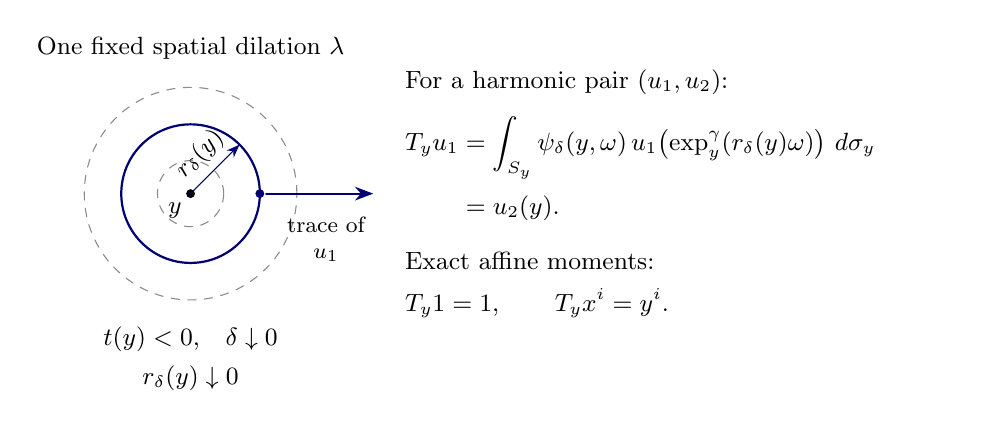
\begin{tikzpicture}[x=1cm,y=1cm,font=\small,>=Stealth,
  line cap=round,line join=round]
  \colorlet{sphereink}{blue!45!black}
  \node at (1.70,2.40) {One fixed spatial dilation $\lambda$};
  \draw[black!45,dashed] (1.70,0.55) circle (1.35);
  \draw[sphereink,thick] (1.70,0.55) circle (0.88);
  \draw[black!45,dashed] (1.70,0.55) circle (0.42);
  \fill (1.70,0.55) circle (1.6pt);
  \node[anchor=north east,inner sep=3pt] at (1.70,0.55) {$y$};
  \draw[->,sphereink] (1.70,0.55)--(2.3223,1.1723);
  \node[rotate=45,anchor=south,inner sep=3pt] at (2.011,0.861) {$r_\delta(y)$};
  \fill[sphereink] (2.58,0.55) circle (1.6pt);
  \draw[->,sphereink,thick] (2.66,0.55)--(4.02,0.55);
  \node[anchor=north,align=center,font=\footnotesize] at (3.42,0.38)
    {trace of\\$u_1$};
  \node[anchor=north,align=center] at (1.70,-1.02)
    {$t(y)<0$,\quad $\delta\downarrow0$\\[3pt]
     $r_\delta(y)\downarrow0$};
  \node[anchor=west,align=left,text width=7.10cm] at (4.30,0.55) {
    For a harmonic pair $(u_1,u_2)$:\\[7pt]
    $\displaystyle
      T_yu_1=\int_{S_y}\psi_\delta(y,\omega)\,
        u_1\!\left(\exp_y^\gamma(r_\delta(y)\omega)\right)
        \,d\sigma_y$\\[5pt]
    $\displaystyle \hphantom{T_yu_1}{}=u_2(y).$\\[9pt]
    Exact affine moments:\\[4pt]
    $\displaystyle T_y1=1,\qquad T_yx^i=y^i.$
  };
\end{tikzpicture}


\caption{A normal-coordinate section of $\gamma$-geodesic spheres in the
first variable, where $\gamma$ is the conformal reference metric.  The
center $y$ satisfies $t(y)<0$.  The spatial dilation $\lambda$ is fixed
while $\delta$ decreases.  The Green functional transfers paired harmonic
functions and reproduces affine harmonic coordinates exactly.  The
unit-sphere measure $d\sigma_y$ has total mass one; the density
$\psi_\delta$ need not be positive.}
\label{fig:shrinking-functional}
\end{figure}
% END work/intake-assessment/manuscript/Smooth-Anisotropic-Uniqueness-in-the-Calderon-Problem-from-One-Boundary-Patch-September-24-2026/build/sections/04-shrinking-balls.tex

% BEGIN work/expanded-manuscript/cross-expanded.tex
\section{Expanded checks for the cross and shrinking-sphere construction}
\label{cross-expanded:section}

This section supplements the retained original Sections 3--4. It records
authoring calculations, not an independent review or a formal proof certificate.
Source labels below refer
to the retained manuscript. Standard analytic interfaces S2--S5 remain subject
to their separate source verification and eventual formal proof. None is a new
authorized axiom. The local metric extension theorem remains a claimed result
until the later angular estimate and bootstrap have been established.

\subsection{The common basis and the exponent margin}
\label{cross-expanded:series}
For \texttt{cross:series}, distributional solution space
$\mathcal H(D)=\{w\in L^2(D):Lw=0\}$ is closed: testing an $L^2$ limit
against $L^*\varphi$, $\varphi\in C_c^\infty(D)$, preserves the equation.
Interior regularity and compact Sobolev embedding make restriction to
$S\Subset D$ compact. Unique continuation makes it injective. The spectral
theorem therefore gives the asserted basis with positive singular values;
there is no omitted zero-eigenspace. A finite-dimensional solution space,
if it occurs, simply gives a finite sum.

To quantify decay, fix a cutoff supported inside $D$, equal to one near
$\overline S$, and a cube containing its support. Interior estimates bound
the cutoff solution in $H^k$ by its $L^2(D)$ norm. Projection onto Fourier
modes $|\xi|\le A$ has rank at most $C A^n$ and error at most $C_k A^{-k}$
in $L^2$. Restriction to $S$ preserves this bound. The minimax principle
gives $\mu_j\le C_k j^{-k/n}$. This uses upper bounds only.

For a slice on $D_1\times S_2$, Parseval gives
$b_j(y)=(F(\cdot,y),w_j)_{D_1}$. Restricting its expansion to $S_1$
and using $(w_i,w_j)_{S_1}=\mu_j^2\delta_{ij}$ proves the coefficient
formula in \texttt{cross:coefficient-extension}. Cauchy--Schwarz gives
$\|b_j\|_{D_2}\le M/\mu_j$. Fubini and testing under the integral
prove $L_2b_j=0$ distributionally. Consequently, with
$\alpha=\gamma_1+\gamma_2-1>0$,
\[
 \|w_jb_j\|_{L^2(O_1\times O_2)}\le CM\mu_j^\alpha,
 \qquad \sum_j\mu_j^\alpha<\infty.
\]
One may choose any integer $k$ with $k\alpha/n>1$. This makes explicit
why a strictly positive exponent margin, rather than its limiting value zero,
is indispensable. Distributional convergence preserves both equations, and
interior estimates for the elliptic sum give the claimed smooth bounds.

The range-completeness check in the source is essential. If
$z\perp\overline{R\mathcal H(D_1)}$, its pairing with the second-piece
slice solves $L_2$ and vanishes on $S_2$, hence on connected $D_2$.
The second-piece slices therefore belong to the closure of that restriction range, as proved in Section~\ref{cross-repairs:range}. Their complete
orthonormal expansion uses $w_j/\mu_j$ and coefficients $\mu_jb_j$.
Absolute convergence on $S_1\times O_2$ follows from
$\sum_j\mu_j^{\gamma_2}<\infty$; on $O_1\times S_2$ it follows from
$\sum_j\mu_j^{\gamma_1}<\infty$. These observations prove agreement on
the actual intersections even if the observed sets are not in the output sets.

For \texttt{cross:exponent}, put $\phi(s)=s-\kappa s^2$. Direct subtraction
gives the exact identity
\begin{equation}\label{cross-expanded:gamma}
 \gamma-\frac12
 =\frac{\kappa l^2-4e+8\kappa e^2}{2l(1-6\kappa e)}.
\end{equation}
Choose the weight and lateral radius first, then $l$ sufficiently small
compared with the lateral quadratic gap, and finally
$0<e\le\kappa l^2/8$ with $6\kappa e<1/2$.
The numerator is then at least $\kappa l^2/2$, so both exponents exceed
one half by a fixed positive amount after these choices are frozen.
The balancing step has the form
$\|w\|_O\le C(e^{-a\tau}+s e^{b\tau})$ for normalized
$\|w\|_D=1$ and $s=\|w\|_S$, with
$a=\phi(-e)-\phi(-l+3e)>0$ and $b=\phi(l+3e)-\phi(-e)>0$.
Taking $\tau=\log(1/s)/(a+b)$ gives $s^{a/(a+b)}$ when
$\tau\ge\tau_0$. Otherwise $s\ge e^{-(a+b)\tau_0}$ and the trivial
$\|w\|_O\le1$ is absorbed by a larger constant. The case $s=0$ follows
from unique continuation. Polynomial Carleman prefactors can be discarded
for $\tau\ge\tau_0\ge1$ in this upper bound.

\subsection{The finite-dimensional separation step}
\label{cross-expanded:dual}
Write $\ell=d\rho$ and normalize dual positive semidefinite tests by
$\operatorname{tr}D=1$. The dual cone of the allowed $i$th weight Hessians
is generated by $a_i\otimes a_i+v_i\otimes v_i$ with
$v_i\perp a_i$, $|v_i|=|a_i|$. Its elements have diagonal blocks
$d_i a_i\otimes a_i+S_i$ with $S_i\ge0$ tangential and
$\operatorname{tr}S_i=d_i|a_i|^2$. This characterization follows by
diagonalizing $S_i$; its eigenvalues express it as a nonnegative sum
of the generating tangential rank-one forms.

Regard $D$ as the covariance of a centered finite-dimensional random vector. This is shorthand for a Gram factorization $D=CC^T$; no probabilistic result is needed for the following matrix calculation.
If $D\ell=0$, the two scalar normal components measured by
$d_x\rho,d_y\rho$ sum to zero almost surely. Their variances are equal,
so $d_1=d_2=d$. The diagonal-block condition says each normal component
is uncorrelated with its own tangent component; the opposite-normal relation
makes it uncorrelated with both. Hence
\[
 D=d(a_1,-a_2)\otimes(a_1,-a_2)+D_\perp,
 \qquad \operatorname{tr}(D_\perp)_{ii}=d|a_i|^2.
\]
If $d=0$, positivity and the trace conditions force $D=0$, a contradiction.
In fact normalization gives $2d(|a_1|^2+|a_2|^2)=1$.
In the compact convex set of admissible $D_\perp$, a matrix of rank
$r\ge2$ is not extreme: the space of symmetric forms on its image has
dimension $r(r+1)/2>2$, leaving a nonzero perturbation preserving both
block traces. Small perturbations of both signs preserve positivity.
Every extreme point thus has rank one and equals
$d(v_1,v_2)\otimes(v_1,v_2)$ with the required lengths. Finite-dimensional
convexity reduces positivity of $H:D$ exactly to
\texttt{cross:hessian-test}.

The set of normalized dual tests is compact. On its subset $D\ell=0$,
$H:D$ has a positive minimum. It remains positive on a neighborhood of
that subset. On the complement, $D:(\ell\otimes\ell)$ has a positive
minimum; choosing $K$ large there makes
$(H+K\ell\otimes\ell):D>0$ on every normalized test. Separation from the
open cone of positive definite forms plus allowed block Hessians yields
the desired $P_1,P_2$. Prescribe their covariant Hessians and the gradients
$d_i\rho$ by quadratic coordinate polynomials. Taylor expansion of
$\rho+K\rho^2/2-\theta_1-\theta_2$, whose value and first derivative
vanish and whose Hessian is positive definite, supplies the quadratic gap.
This proves the linear-algebra step rather than assuming a splitting theorem.

\subsection{The tube geometry and its parameter order}
\label{cross-expanded:tubes}
For \texttt{cross:tubes}, write $r=a t^{1+\sigma}$ and
$t=M+y_n+e_0|y'|^2$. Differentiation gives
\[
 b=(1+\sigma)\frac r t\,dt,\qquad
 r\partial^2r=\frac{\sigma}{1+\sigma}b\otimes b
                +(1+\sigma)\frac{r^2}{t}\partial^2t.
\]
Since $|dt|\ge1$, $\|\partial^2t\|=2e_0$, and $t\le T_0$, the second
term is bounded by $C T_0e_0|b|^2$. Outside the seed,
$y_n\ge c_0r$ gives $r/t\le1/c_0$, hence a bounded $b$-range.
The zero cases for the projected square are $b=0,-2\omega$;
$b=-\omega$ is separately excluded because the second partial gradient
vanishes. Near $b=0$, the real projection controls $b$ perpendicular
to $\omega$, and the change in imaginary projected length controls its
parallel component. Thus the lower bound is $c|b|^2$ there as well.

The parameter order avoids circular dependence. Fix the coarse-seed
constant $c_0$, $M>B+3$, and the two excluded-neighborhood sizes first.
Choose $\sigma>0$ small. Restrict eventually to
$e_0\le1/(1+B^2)$, so target values of $t$ have a fixed upper bound.
Choose $a_{\min}>0$ small enough to lie below all target separations,
and $a_{\max}$ large enough for its level to lie in the seed. Next choose
$T_0$ with $c_0a_{\min}T_0^\sigma>1$. Finally choose $e_0$ so small that
$T_0e_0$ and $\sqrt{T_0e_0}$ satisfy the required error margins.
The transverse base may become very large, but is still compact; only
after fixing it is the dilation $\lambda$ chosen. Near $b=-\omega$ or
$b=-2\omega$, the inequality
$x_n/r\le(1+\sigma)|dt|/|b|+\omega_n$ places the pair in the seed
for these choices. On the remaining range the displayed Hessian error
is absorbed by $c|b|^2$. Its strict margin is positive on the compact
non-seed cylinder. This argument gives no uniform estimate as the
prescribed separation tends to zero.

\subsection{Profile bounds and the moving-sphere cancellation}
\label{cross-expanded:spheres}
For \texttt{balls:profiles}, put $z=e^{t/\delta}$.
Logarithmic differentiation of
$A=z/((1+z)\log(1+z))$ gives
$A'/A=(1-z/\log(1+z))/(1+z)<0$.
At the negative end $A=1+O(e^s)$; at the positive end
$A=s^{-1}(1+O(e^{-s}(1+s)))$. Differentiating these convergent
expressions gives $|A^{(j)}|\le C_j A^{j+1}$, with the remaining
compact interval covered by positivity. Thus the chain rule and the fixed
upper and lower bounds on $|dt|_\gamma$ give the stated derivative bounds
for $f=p\log\ell+\log R_*$. The factor $p$ is absorbed into $p^j$ for
$j\ge1$. Also $a=\ell'/\ell\le1/\ell$, so
$r\beta^2\le C R_*p^2\ell^{p-2}$; this is uniform in $\delta$ for fixed
$p\ge2$. The derivative in $\delta$ of $\ell$ is positive, since its
derivative as a function of $s$ is $-s e^s/(1+e^s)^2$ and its two endpoint
limits are zero. These calculations justify monotonicity used in propagation.

For \texttt{balls:test-expression}, all complex quadratic expressions
mean the real form evaluated on a vector and its conjugate. Since
$\omega\cdot(U_1-U_2)=b\cdot U_2$ and
$\operatorname{Hess}(r^2/2)=2dr\otimes dr+r^2\operatorname{Hess}f$,
the positive normal square in the distance Hessian cancels one of the
two copies of $|b\cdot U_2|^2$. The surviving expression is exactly
the projected square minus $|b\cdot U_2|^2$ minus the Hessian term.
The real projection is $-b_\perp+O(|b|^2+|h|)$, while the reverse triangle
inequality for imaginary projections gives a square at least
$(\omega\cdot b)^2-C(|b|^3+|b||h|+|h|^2)$.
The two real directions of $U_2$ are orthogonal up to $O(|h|)$, with
lengths $1+O(|b|+|h|)$, so Bessel's inequality with this perturbation
bounds $|b\cdot U_2|^2$ by $(1+C(|b|+|h|))|b|^2$.
Finally $|h|+|\partial h|\le C\varepsilon r$ makes the connection
error $O(\varepsilon r^2)$, and the Jacobi-field error is $O(r^2)$.
The resulting lower bound is
$cr^2\beta-C(r^2+r^3\beta^3+\varepsilon r^2\beta+\varepsilon^2r^2)$.
Choose $p$ first so that the lower bound for $\beta$ absorbs $Cr^2$,
then $\varepsilon$, then $R_*$ so that $r\beta^2\le\varepsilon$.
The spatial dilation is chosen last and remains fixed while $\delta$
decreases. The temporary $H_8$ inequality is a hypothesis at this stage.

\subsection{Flux density and the exact remaining obligations}
\label{cross-expanded:flux}
Let $k_y$ be the boundary value of the mixed kernel and let $\Lambda_y$
be the Dirichlet-to-Neumann map on the first-metric ball. Green's identity
makes $\Lambda_y$ self-adjoint with respect to $dS_1$. If the sphere
parametrization pulls $dS_1$ back to $J_y\,d\sigma_y$, the density is
explicitly $\psi=J_y(\Lambda_y k_y-\partial_{\nu_1}\mathcal G)$.
The sign gives $T_yu=u(y)$ when the kernel is the positively normalized
inverse of $-\Delta_{g_1}$, because Green's second identity then has
integrand $G\partial_\nu u-u\partial_\nu G$.
For a fixed center, compactness of its sphere gives a common open collar
in the kernel domain. A slightly larger fixed surface in this collar
surrounds all sufficiently nearby moving spheres. Green's identity in
the intervening annulus fixes the integration surface; applying $L_2$
under that integral proves local harmonicity of $T_yu$. Unique continuation
from the known lower region then gives reproduction for every fixed paired
harmonic function, including constants and coordinates.

The cutoff bounds require parameter-dependent smooth Dirichlet regularity
on a fixed unit ball after rescaling, including the center evaluation
kernel and its angular derivatives. On the lower region the limiting
principal metric is a scalar multiple of the Euclidean one, because
$\gamma$ is conformal to $g_1$; the limiting harmonic equation is therefore
Euclidean. Center differentiation introduces $dr$, bounded by $r\beta$.
On $t>t_b$ the fixed positive lower radius permits fixed-separation Green
bounds instead. These uses belong to S2, S3 and S5 and require precise
interfaces with uniform constants. S4 supplies unique continuation and
the strict-weight Carleman estimate. The common-basis spectral theorem
belongs to S5. Exact published locators remain pending separately from
the derivations above; monographs are preferred and no lecture notes
have been adopted. Sections 3--4 give only conditional existence of the
sphere transfer, not its uniform norm at shrinking radius. The latter
and closure of $H_8\le\varepsilon r_\delta$ remain the substantive
downstream obligations. No contradiction in the calculations checked
here was identified; that observation is not a proof of the frozen theorem.
% END work/expanded-manuscript/cross-expanded.tex

% BEGIN work/intake-assessment/manuscript/Smooth-Anisotropic-Uniqueness-in-the-Calderon-Problem-from-One-Boundary-Patch-September-24-2026/build/sections/05-angular-estimate.tex
\section{An estimate on the shrinking spheres}
\label{sec:angular}

The functional in Proposition~\ref{balls:functional} is defined at every positive
radius.  We now estimate its representing density uniformly as the radius
shrinks.  The equation for this density has second-order angular and base
terms.  Comparing a degree-raising operator with a degree-lowering operator
will control both kinds of derivatives; a second comparison will retain the
principal terms caused by the changing metric.

\subsection{The equation for the density}

We use the reference metric $\gamma$, the normalized second principal
matrix $Q$, and $h=Q-\gamma^{-1}$ from
\eqref{balls:normalization}.  In this section the subscript $\delta$ on the positive
radius $r$ is suppressed.  Put
\[
 f=\log r,\qquad \beta=|df|_\gamma.
\]
The required profile bounds are
\begin{equation}\label{angular:profile-bounds}
 \beta\ge\beta_0,\qquad
 \operatorname{Hess}_\gamma f\le-c_0\beta\gamma,
 \qquad |\nabla^j f|\le C_j\beta^j\quad(1\le j\le8),
\end{equation}
where $c_0>0$ and $C_j$ are fixed.  Lemma~\ref{balls:profiles} provides
these bounds with $\beta_0$ arbitrarily large by choosing $p$
sufficiently large.  All background metric bounds
below are on a fixed relatively compact coordinate region; their constants
are uniform in the spatial dilation.

Let $S_\gamma Y$ be the bundle of $\gamma$-unit tangent spheres over the
base region $Y$.  Each sphere has probability measure $d\sigma_y$.
Horizontal differentiation $\nabla$ uses parallel transport for $\gamma$,
including the covariant tensor indices of an operator or section.  This
connection preserves the sphere measure.  Unless otherwise specified, all
norms and full adjoints use $dV_\gamma(y)\,d\sigma_y(\omega)$.

On each tangent unit ball, extend a sphere function harmonically for the
Euclidean metric $\gamma(y)$.  Denote the boundary radial derivative of
this extension by $B$, and its ambient derivatives in an orthonormal frame
by $A_i$.  Thus $B=k$ on the space $\mathcal H_k$ of spherical harmonics
of degree $k$, and $A_i:\mathcal H_k\to\mathcal H_{k-1}$.  The star in
$A_i^*$ denotes the sphere adjoint.  These operators are parallel, with
the indicated tensor indices, and
\begin{equation}\label{angular:elementary-identities}
 [B,A_i^*]=A_i^*,\qquad \sum_i A_i^*A_i^*=0.
\end{equation}
Indeed differentiation lowers homogeneous degree by one, and the second
identity is the adjoint of the vanishing Laplacian of a harmonic extension.
For $s\in\mathbb R$, use the fiber Sobolev norm
\[
 \|v(y,\cdot)\|_s=\|(1+B)^s v(y,\cdot)\|_{L^2(S_y)}.
\]
It is equivalent to the usual Sobolev norm on the unit sphere.  Tensor-valued
versions use the sum over an orthonormal frame.

We write $\Psi^m$ for the classical pseudodifferential operators of order
$m$ on the sphere.  For a positive function $a(y)$, the notation
$a\Psi^m$ means that, after division by $a$, the finitely many symbol and
operator seminorms used below are bounded.  A statement with $j$ base
derivatives permits the indicated additional factor $\beta^j$.

\begin{lemma}[Moving trace operators]\label{angular:trace}
Suppose that the normal balls and the functional $T_y$ of
Proposition~\ref{balls:functional} are defined, and that
\begin{equation}\label{angular:smallness}
 \sum_{|\alpha|\le8}|\partial_y^\alpha h|\le\eps r,
 \qquad r\beta^2\le\eps.
\end{equation}
If $u$ is first-metric harmonic near one such ball, set
\[
 U(y,\omega)=u\bigl(\exp_y^\gamma(r(y)\omega)\bigr).
\]
There are sphere operators $\mathcal C_i$ such that
$\nabla_iU=\mathcal C_iU$.  Their sphere adjoints satisfy
\begin{equation}\label{angular:C-expansion}
 \mathcal C_i^*=r^{-1}A_i^*+f_iB+E_i+F_i,
 \qquad E_i\in r\Psi^1,\quad F_i\in\Psi^0,
 \qquad f_i=\nabla_i f.
\end{equation}
The normalized remainders $r^{-1}E_i$ and $F_i$ have uniform symbol
bounds after up to six base derivatives, with the allowance $C_j\beta^j$.

Write the normalized second equation, in the reference connection, as
$Q^{ij}\nabla_i\nabla_j+b_2^i\nabla_i$.  Its drift $b_2$ is uniformly
controlled.  If $\psi(y,\omega)$ represents $T_y$ against $d\sigma_y$,
then
\begin{equation}\label{angular:P-equation}
 P\psi=0,\qquad
 P=r\left[Q^{ij}(\nabla_i+\mathcal C_i^*)
                    (\nabla_j+\mathcal C_j^*)
             +b_2^i(\nabla_i+\mathcal C_i^*)\right].
\end{equation}
The products in this formula are covariant products.  In particular,
$Q$ is not differentiated by taking a base adjoint.
\end{lemma}

\begin{proof}
Normalize the principal part of the first equation to $\gamma^{-1}$ and
pull it back by $z\mapsto\exp_y^\gamma(rz)$ to the unit ball.  After
multiplication by $r^2$, its principal coefficients are
$\delta^{ij}+O(r^2)$ and its first-order coefficients are $O(r)$.
The resulting smooth family remains uniformly elliptic and has an
invertible Dirichlet problem, including at $r=0$.  Its radial derivative
operator therefore has the expansion
\begin{equation}\label{angular:radial-expansion}
 B+r B_1(y)+r^2 B_2(y,r),\qquad
 B_1\in\Psi^0,\quad B_2\in\Psi^1.
\end{equation}
Here is the parameter justification.  The classical boundary-symbol
construction is described in
\citep[Theorem~1.1(i) and Proposition~3.1]{JoshiLionheart2005};
we keep the center and radius dependence explicitly.
In boundary coordinates the decaying
normal root of the principal symbol constructs the Dirichlet parametrix.
Successive lower-order transport equations construct its symbols smoothly
in $(y,r)$.  The first normal derivative trace is an operator of order one,
whose principal symbol depends only on the principal coefficients and the
differentiating vector.  Those coefficients have zero first $r$-derivative
at $r=0$, so that derivative of the trace operator has order zero.  Taylor's
formula in this symbol class gives \eqref{angular:radial-expansion} to
smoothing error.  The true solution differs from the parametrix by the
Dirichlet inverse of a smooth error; differentiated Dirichlet estimates
control this remainder in every fixed seminorm.  More explicitly, on a
compact center set the rescaled Dirichlet operator is smoothly
invertible between each fixed pair of Sobolev spaces, uniformly for
$0\le r\le r_0$.  Differentiating that inverse controls every fixed
number of parameter derivatives of the smoothing correction; increasing
the Sobolev orders controls its smooth kernel seminorms.  Thus the
Taylor expansion holds in the complete classical symbol topology,
including the smoothing remainder, and not merely in one Sobolev
operator norm.  This proves the stated expansion and its parameter bounds.

Differentiate the exponential map in its center, transporting $\omega$
parallel to the center velocity.  The Jacobi field has initial derivative
zero.  After inverting the differential in the $z$ variable, the velocity
acting on the unit-ball solution is
\[
 r^{-1}\bigl(e_i+O(r^2)\bigr)+f_i\omega.
\]
The coefficient error is smooth in $(y,r,\omega)$.  Tangential derivatives
act directly on the boundary value; the radial derivative is
\eqref{angular:radial-expansion}.  At $r=0$ the first term is $r^{-1}A_i$.
The order-one errors are $O(r)$, and the order-zero errors are bounded:
in particular $r f_i B_1$ is bounded because $r\beta\le\eps/\beta$.
Taking sphere adjoints gives \eqref{angular:C-expansion}.  Differentiating
the radius costs at most one factor $\beta$ per derivative, by
\eqref{angular:profile-bounds}; the asserted parameter estimates follow.

For fixed $u$, differentiate
$T_yu=\langle\psi(y,\cdot),U(y,\cdot)\rangle_{S_y}$.
Metric compatibility and $\nabla_iU=\mathcal C_iU$ put the differentiated
operator on $\psi$ as $\nabla_i+\mathcal C_i^*$.
The local second-metric harmonicity in
Proposition~\ref{balls:functional} proves that
\eqref{angular:P-equation} pairs to zero with the trace of every
function harmonic near the fixed closed ball.  No global extension
or source-family approximation is used in this step.
At a fixed sphere these traces are dense among
smooth boundary data: solve the smooth Dirichlet problem on slightly
enlarged balls, using boundary values transported from the limiting sphere,
and use smooth dependence of the solution on the radius.  Thus the paired
equation is the stated equation for $\psi$.
\end{proof}

\subsection{The model operator and its principal perturbations}

We separate a degree-raising model operator from the remaining
principal and lower-order terms of the moving trace equation.  We continue under the hypotheses of
Lemma~\ref{angular:trace}, including \eqref{angular:smallness}.

Define
\begin{equation}\label{angular:T-definition}
 D_i^+=\nabla_i+f_iB,\qquad D_i^-=-\nabla_i+f_iB,
 \qquad
 T=\sum_i A_i^*D_i^+,\quad T^\flat=\sum_i A_iD_i^-.
\end{equation}
The symbol $T$ here denotes a differential operator on sphere functions;
the transfer functional continues to be denoted $T_y$.
Expand \eqref{angular:P-equation} by
\eqref{angular:C-expansion}.  The identities
\eqref{angular:elementary-identities} give
\[
 D_i^+(r^{-1}A_j^*)=r^{-1}A_j^*D_i^+,
 \qquad \sum_iA_i^*A_i^*=0.
\]
Thus, in ordinary base coordinates and an orthonormal sphere
trivialization,
\begin{equation}\label{angular:P-decomposition}
 P=2T+U+J,
\end{equation}
where $J$ is a uniformly bounded family in $\Psi^1$, with no base
derivatives, and
\begin{equation}\label{angular:U-bounds}
 U=\sum_{|\alpha|\le2}U_\alpha(y)\partial_y^\alpha,
 \qquad U_\alpha\in\eps\beta^{-|\alpha|}
                               \Psi^{2-|\alpha|}.
\end{equation}
Up to five derivatives of these coefficients have the additional
allowance $C_j\beta^j$.  The second-base-derivative term is precisely
\begin{equation}\label{angular:real-principal-part}
 rQ^{ij}\partial_{y_i}\partial_{y_j};
\end{equation}
its coefficients are real scalars independent of the sphere variable.

We detail these bounds.  The pure angular second derivative contracted
with $\gamma^{-1}$ vanishes.  The remaining contraction is
$(h^{ij}/r)A_i^*A_j^*$, and belongs to the zero-base-derivative term of
\eqref{angular:U-bounds}.  The mixed correction is
$2h^{ij}A_i^*D_j^+$ and has the stated small bounds.  The $D^+D^+$ term
has coefficient $r$; its base orders two, one and zero have coefficients
$O(r)$, $O(r\beta)$ and $O(r\beta^2)$, respectively.  The condition
$r\beta^2\le\eps$ gives \eqref{angular:U-bounds} for all three.
Terms containing $E_i$ obey the same bounds.  Terms containing $F_i$
also do so, except for their cross terms with $r^{-1}A_j^*$, which are
bounded angular order-one terms and belong to $J$.  The drift term with
$A_i^*$ belongs to $J$ as well.  Differentiating any of these expressions
gives the stated coefficient bounds by
\eqref{angular:profile-bounds} and \eqref{angular:smallness}.
A horizontal connection written in this trivialization adds a bounded
angular first derivative, which preserves the same estimates.  The bounds
for $J$ use the fixed background and remain uniform as $\beta_0$ is
increased.

The decomposition identifies the model operator $2T$ and the
second-order perturbation $U$.  To carry the model estimate over to $P$
we shall need more than an ordinary first-derivative estimate: the error forms
also contain mixed base and angular derivatives.  For a sphere function
$\varphi$, put
\begin{equation}\label{angular:N-definition}
 \mathcal N(\varphi)^2
 =\int_Y\left(
  \|\nabla\varphi\|_0^2+\beta^2\|\varphi\|_1^2
  +\beta^{-1}\|\nabla\varphi\|_{1/2}^2
  +\beta\|\varphi\|_{3/2}^2\right)dV_\gamma.
\end{equation}

The last two terms of $\mathcal N$ place half an angular derivative
on $\nabla\varphi$ and three halves on $\varphi$.  They will bound the
remaining error forms left by the comparison with $P$.

\subsection{A comparison of raising and lowering operators}

The next estimate supplies these two derivative strengths for the model
operator.  Spherical harmonics are trace-free symmetric tensors, and
comparing their raising and lowering operators is familiar from energy
identities in tensor tomography; see, for example, \cite{PSU15,GPSU16}.
Here the negative Hessian of the spatial weight supplies the positive
term that absorbs the bounded curvature.  We give the calculation with
its degree factors.

\begin{lemma}[Weighted raising estimate]\label{angular:raising}
Let $n\ge3$, and suppose \eqref{angular:profile-bounds} holds on a fixed
base region with uniformly bounded reference geometry.  There are
$\beta_0$ and $c>0$, depending only on that geometry and the constants in
\eqref{angular:profile-bounds}, such that every smooth, compactly
base-supported function with zero fiber mean satisfies
\begin{equation}\label{angular:raising-estimate}
 \|T\varphi\|^2-\|T^\flat\varphi\|^2
       \ge c\,\mathcal N(\varphi)^2.
\end{equation}
\end{lemma}

\begin{proof}
Both operators change angular degree by exactly one, so it suffices to
prove the estimate at one input degree $k\ge1$.  Identify that component
with a harmonic homogeneous polynomial $v(z)$ of degree $k$.  Use the
Fischer inner product, in which the monomials $z^\alpha$ are orthogonal
with squared norm $\alpha!$.  Polynomial differentiation $a_i=\partial_{z_i}$
is adjoint to multiplication $M_i=z_i$.  On harmonic polynomials of degree
$k$ the Fischer squared norm is the normalized squared sphere norm
multiplied by
\[
 N_k=n(n+2)\cdots(n+2k-2),\qquad N_0=1.
\]
For completeness, integration against a standard real Gaussian identifies
the Fischer norm on trace-free homogeneous polynomials with their
Gaussian $L^2$ norm;
integrating radially then gives the factor $N_k$.  These classical
identities are also recorded in \cite[Equation~(2.1) and
Theorem~2.1]{Render08}.

Set $d=k+n/2-1$ and use $D_i^\pm=\pm\nabla_i+k f_i$ at this fixed degree.
For harmonic polynomials $q_i$ of degree $k$, the Laplacian of
$\sum_iM_iq_i$ is $2\sum_i a_iq_i$.  Since
\[
 \Delta_z(|z|^2s)=4d\,s\qquad(s\in\mathcal H_{k-1}),
\]
its harmonic projection is
$\sum_iM_iq_i-|z|^2\sum_i a_iq_i/(2d)$.  Orthogonality of this projection
and its complement shows that its squared norm is
\[
 \sum_i\|q_i\|^2+\sum_{i,j}(a_jq_i,a_iq_j)
             -d^{-1}\Bigl\|\sum_i a_iq_i\Bigr\|^2.
\]
Changing from Fischer adjoints to sphere adjoints gives
\[
 A_i^*|_{\mathcal H_k}
   =\frac{N_{k+1}}{N_k}\Pi_{k+1}M_i,
\]
where $\Pi_{k+1}$ is harmonic projection in homogeneous degree $k+1$.
Consequently $N_k$ times the left side of
\eqref{angular:raising-estimate} is
\begin{equation}\label{angular:Fock-difference}
 \begin{split}
 (2d+2)\left[\|D^+v\|^2
   +\sum_{i,j}(a_jD_i^+v,a_iD_j^+v)
   -\frac1d\Bigl\|\sum_i a_iD_i^+v\Bigr\|^2\right]
 -2d\Bigl\|\sum_i a_iD_i^-v\Bigr\|^2.
 \end{split}
\end{equation}
All norms in this calculation include integration over the base and use
the polynomial inner product in the fibers.  The factors are
$N_{k+1}/N_k=2d+2$ and $N_k/N_{k-1}=2d$.

Write $C_{ij}=2k(\operatorname{Hess}_\gamma f)_{ij}$ and
\[
 C[av]=\int_Y\sum_{i,j}C_{ij}\langle a_iv,a_jv\rangle\,dV_\gamma.
\]
Covariant integrations by parts give
\begin{align}
 \sum_{i,j}(a_jD_i^+v,a_iD_j^+v)
   &=\Bigl\|\sum_i a_iD_i^-v\Bigr\|^2-C[av]
                                    +O(k^2)\|v\|^2,\label{angular:ibp-one}\\
 \Bigl\|\sum_i a_iD_i^+v\Bigr\|^2
   &\le k\|D^-v\|^2-C[av]+O(k^2)\|v\|^2,\label{angular:ibp-two}\\
 \|D^-v\|^2
   &=\|D^+v\|^2+\int_Y\tr C\,|v|^2\,dV_\gamma.
                                                    \label{angular:ibp-three}
\end{align}
Here and below a form denoted $O(k^2)\|v\|^2$ has absolute value at most
a fixed constant times that quantity.  To verify the first two formulas,
move a $D_j^+$ across the pairing and commute
$D_j^-D_i^+$ to $D_i^+D_j^--C_{ij}$.  The reordered term in
\eqref{angular:ibp-two} is at most $k\|D^-v\|^2$, because
$\sum_i|a_iw|^2=k|w|^2$ for $w\in\mathcal H_k$.
The extra commutator is curvature: it acts as a sum of rotations of norm
$O(k)$ at degree $k$, and the two contractions supply one more factor $k$.
This proves the claimed error bounds.  Expanding the two squares proves
\eqref{angular:ibp-three}.  For complex functions all the displayed forms
are understood through their real parts.

Substituting \eqref{angular:ibp-one} into
\eqref{angular:Fock-difference} rewrites that expression as
\begin{equation}\label{angular:after-first-ibp}
 \begin{split}
 &(2+2/d)\left[d\|D^+v\|^2
       -\Bigl\|\sum_i a_iD_i^+v\Bigr\|^2-dC[av]\right]\\
 &\qquad+2\Bigl\|\sum_i a_iD_i^-v\Bigr\|^2
                      +O(k^3)\|v\|^2.
 \end{split}
\end{equation}
We must control the remaining negative divergence square while retaining
both an ordinary derivative estimate and an additional half-order
angular derivative estimate.  The latter requires a coefficient of
size $k/\beta$ in front of $|D^+v|^2$, including when $k$ is much larger
than $\beta$.  Choose a small constant $\vartheta>0$.
On the fraction $1-\vartheta$ of its negative divergence square use
\eqref{angular:ibp-two}--\eqref{angular:ibp-three}.  On the remaining
fraction use the pointwise convex combination
\begin{equation}\label{angular:convex-bound}
 \begin{split}
 \Bigl|\sum_i a_iD_i^+v\Bigr|^2
 &\le(1-\zeta)(k+n-1)|D^+v|^2\\
 &\quad+\zeta\left(2\Bigl|\sum_i a_iD_i^-v\Bigr|^2
                         +8k^3\beta^2|v|^2\right),
 \qquad \zeta=c_1/\beta.
 \end{split}
\end{equation}
The fraction $1-\vartheta$ in the integrated estimates is constant;
the $y$-dependent $\zeta$ is used only in this pointwise inequality.
The first bound follows from the adjoint multiplication operators, since
the contraction $(q_i)\mapsto\sum_i a_iq_i$ has squared norm at most
$k+n-1$ on polynomials of degree $k$.  The second follows from
$D_i^++D_i^-=2k f_i$ and
$|\sum_i f_i a_i v|^2\le k\beta^2|v|^2$.

Combining these bounds in \eqref{angular:after-first-ibp}, the coefficient
retained for $|D^+v|^2$ is
\begin{equation}\label{angular:positive-degree-factor}
 (2+2/d)\bigl[d-k-\vartheta(n-1)
                         +\vartheta\zeta(k+n-1)\bigr].
\end{equation}
Since $d-k=(n-2)/2$, a sufficiently small fixed $\vartheta$ makes this
at least a fixed positive constant plus a positive multiple of
$c_1k/\beta$.  The coefficient of
$|\sum_i a_iD_i^-v|^2$ is nonnegative when $\beta_0$ is sufficiently
large.  The Hessian contribution is exactly
\begin{equation}\label{angular:hessian-contribution}
 -(2+2/d)\left[(d-1+\vartheta)C[av]
       +(1-\vartheta)k\int_Y\tr C\,|v|^2\,dV_\gamma\right].
\end{equation}
For $k\ge1$ and $n\ge3$, both coefficients inside this expression are
positive.  The Hessian hypothesis bounds it below by
$c k^3\int\beta|v|^2$.  This absorbs the curvature error $O(k^3)\|v\|^2$
by increasing $\beta_0$, and absorbs the last term of
\eqref{angular:convex-bound} by choosing $c_1$ sufficiently small.
We have therefore retained positive multiples of
\[
 \|D^+v\|^2,\qquad
 \int_Y\frac{k}{\beta}|D^+v|^2\,dV_\gamma,
 \qquad k^3\int_Y\beta|v|^2\,dV_\gamma.
\]
The first controls both $\|\nabla v\|^2$ and
$k^2\int\beta^2|v|^2$, since its cross term is
$-k\int\Delta_\gamma f\,|v|^2\ge0$.  For the weighted derivative use the
pointwise inequality
\[
 \frac{k}{\beta}|\nabla v|^2
 \le2\frac{k}{\beta}|D^+v|^2+2k^3\beta|v|^2.
\]
No differentiation of $\beta^{-1}$ is required.  Dividing by $N_k$, and
then summing the orthogonal degree components, proves
\eqref{angular:raising-estimate}; the weights $(1+k)^s$ are comparable
to $k^s$ because the zero degree is excluded.
\end{proof}

\subsection{Keeping the principal perturbations}

The raising estimate controls the model operator.  The actual equation
\eqref{angular:P-equation} also contains second base derivatives and a
small second-order angular perturbation.  We retain these terms in a
comparison of squared norms.

\begin{proposition}[Coercivity for the moving trace equation]
\label{angular:coercivity}
Fix a base region with bounded reference geometry and the constants in
\eqref{angular:profile-bounds}.  Suppose $P$ is the operator
\eqref{angular:P-equation}, with the trace operators of
Lemma~\ref{angular:trace}.  There exist $\beta_0$ sufficiently large,
$\eps_0>0$ and $C<\infty$, depending only on these fixed bounds, such that
\eqref{angular:smallness} with $\eps\le\eps_0$ implies
\begin{equation}\label{angular:coercive-estimate}
 \mathcal N(\varphi)\le C\|P\varphi\|
\end{equation}
for every smooth, compactly base-supported function $\varphi$ with
zero mean on each sphere.  These constants are independent of the
shrinking parameter.  Only the eight indicated derivatives of the small
tensor $h$ are required.
\end{proposition}

\begin{proof}
Let a dagger denote the full adjoint for $dV_\gamma d\sigma$.
Covariant integration and the degree shift give
\begin{equation}\label{angular:Z-definition}
 Z:=T^\flat-T^\dagger=\sum_i f_iA_i.
\end{equation}
A direct expansion yields
\begin{equation}\label{angular:norm-comparison}
 \begin{split}
 &\|(2T+U)\varphi\|^2-
                \|(2T^\flat+U^\dagger)\varphi\|^2\\
 &\qquad=4\bigl(\|T\varphi\|^2-\|T^\flat\varphi\|^2\bigr)
                       +\langle\mathcal E\varphi,\varphi\rangle,
 \end{split}
\end{equation}
where
\begin{equation}\label{angular:error-operator}
 \mathcal E=2[T^\dagger,U]+2[U^\dagger,T]+[U^\dagger,U]
                       -2\bigl(UZ+(UZ)^\dagger\bigr).
\end{equation}
We will prove
\begin{equation}\label{angular:error-form-bound}
 |\langle\mathcal E\varphi,\varphi\rangle|
                         \le C\eps\mathcal N(\varphi)^2.
\end{equation}

Here are the complete order and weight counts needed for this claim.
An operator has count $(m,s)$ if its coefficient at $\partial_y^\alpha$
is angular order $m-|\alpha|$, of size $O(\beta^{s-|\alpha|})$,
with the derivative allowances already specified.
Adjoints preserve the count, and products add the counts.  When a base
derivative hits a coefficient it consumes one differential order and
adds a factor $\beta$, so it preserves the weight index.  A commutator
of scalar angular operators loses one angular order: the products of
their principal symbols cancel.  Hence a scalar commutator loses one in
total order while preserving the sum of the weight indices.
The counts of $T,T^\dagger,U,Z$ are, respectively,
\[
 (2,1),\quad(2,1),\quad(2,0),\quad(1,1),
\]
and every occurrence of $U$ carries the factor $\eps$.  Thus
\eqref{angular:error-operator} has count at most $(3,1)$ and a factor
$O(\eps)$; the quadratic $U$ term is smaller.

There is a further cancellation that the total count alone does not
express: no third base derivative survives.  To check it explicitly,
use an orthonormal sphere trivialization and write the base measure as
$\mu(y)\,dy$.  The sphere probability measure is then fixed.  Write
\[
 U=a^{ij}\partial_i\partial_j+\mathcal B^i\partial_i+\mathcal C,
 \qquad a^{ij}=rQ^{ij}=a^{ji}\in\mathbb R.
\]
The coefficients $\mathcal B^i$ and $\mathcal C$ are angular
operators.  Replacing a horizontal derivative by a coordinate derivative
plus its angular connection term changes only base orders at most one,
so these are all the second-base coefficients.  If a star denotes the
sphere adjoint, direct integration by parts gives
\begin{align*}
 U^\dagger-U
 ={}&\left(2\mu^{-1}\partial_j(\mu a^{ij})
                -\mathcal B^i-(\mathcal B^i)^*\right)\partial_i\\
 &+\mu^{-1}\partial_i\partial_j(\mu a^{ij})
       -\mu^{-1}\partial_i\bigl(\mu(\mathcal B^i)^*\bigr)
       +\mathcal C^*-\mathcal C.
\end{align*}
In particular it has base order at most one.
In $[T^\dagger,U]$ and
its partner, the possible third-base-derivative coefficient is a commutator of an angular coefficient
with $rQ^{ij}$, which is zero by
\eqref{angular:real-principal-part}.  For $[U^\dagger,U]$, first write
it as $[U^\dagger-U,U]$.  The operator $U^\dagger-U$ has no second base
derivative, since the coefficient in
\eqref{angular:real-principal-part} is real.  Taking adjoints against
the smooth base density only produces lower base orders.  Its remaining
possible third-base-derivative coefficients commute for the same reason.
Finally, $UZ$ already has at most two base derivatives.
It follows that $\mathcal E$ is a sum of terms of precisely the following
three permitted types:
\begin{equation}\label{angular:error-types}
 \eps\beta^{-1}\Psi^1\partial_y^2,
 \qquad \eps\Psi^2\partial_y,
 \qquad \eps\beta\Psi^3.
\end{equation}
This argument also covers lower orders, since $\beta\ge1$.

For the first type in \eqref{angular:error-types}, integrate once in the
base.  The principal form is bounded by
$C\eps\int\beta^{-1}\|\partial_y\varphi\|_{1/2}^2$.
A derivative of its coefficient costs one factor $\beta$ and leaves an
$\eps\Psi^1\partial_y$ term.  This includes differentiation of the
weight itself: $|d\beta|\le C\beta^2$ implies
$|d(\beta^{-1})|\le C$.  The second type has the form bound
\[
 C\eps\int_Y
     \|\partial_y\varphi\|_{1/2}\|\varphi\|_{3/2}\,dV_\gamma
 \le C\eps\int_Y\left(
     \beta^{-1}\|\partial_y\varphi\|_{1/2}^2
                 +\beta\|\varphi\|_{3/2}^2\right)dV_\gamma.
\]
The third type is bounded by
$C\eps\int\beta\|\varphi\|_{3/2}^2$.
The lower-order term from differentiating a coefficient satisfies the
same bound.  Replacing coordinate derivatives by horizontal derivatives
adds a bounded angular first derivative, again controlled by these norms.
A fixed finite partition of the base region has the same harmless
lower-order errors.  This proves \eqref{angular:error-form-bound}.

The constants in the preceding estimates are uniform for all
$\beta\ge\beta_0$ once a fixed lower threshold is met.  Choose
$\eps_0$ small relative to the constant in
Lemma~\ref{angular:raising}.  Dropping the nonnegative second squared
norm in \eqref{angular:norm-comparison} gives
$\mathcal N(\varphi)\le C\|(2T+U)\varphi\|$.
Finally,
\[
 \|J\varphi\|\le C\|\varphi\|_{L^2(Y;H^1(S_y))}
                         \le C\beta_0^{-1}\mathcal N(\varphi),
\]
so a sufficiently large $\beta_0$ absorbs $J$ and proves
\eqref{angular:coercive-estimate}.

All these operations use angular symbol estimates pointwise in the base,
and ordinary base differential operators of degree at most two.  Formal
adjoints, the commutator expansion and the one integration by parts use
at most the five base coefficient derivatives specified in
\eqref{angular:U-bounds}.  Construction of these coefficients differentiates
the moving trace operators once and the second metric to only finitely
many orders below eight.  Higher angular symbol seminorms depend on the
fixed smooth first-metric family; differentiating in the angular variable
does not differentiate the center-dependent tensor $h$.  Thus the eight
smallness derivatives in \eqref{angular:smallness} suffice in every fixed
dimension.  No smallness assumption on all derivatives of $h$ is used.
\end{proof}

\subsection{The constant mode and the uniform density bound}

We now apply the coercive estimate to the transfer density constructed in
Section~\ref{sec:balls}, restoring the notation $r=r_\delta$.
Its normalization is $\int_{S_y}\psi\,d\sigma_y=1$, so
$\chi(\psi-1)$ has zero fiber mean for the fixed cutoff
\eqref{balls:cutoff-region}.  This is the mean-zero condition required
by Proposition~\ref{angular:coercivity}.

The decomposition \eqref{angular:P-decomposition} gives a uniform
bound for $P1$: its raising part annihilates $1$, only $U$'s bounded
zero-base-derivative coefficient acts on $1$, and $J$ is uniformly
bounded in $\Psi^1$.  There is no factor growing with $\beta$ in this
assertion.

For any fixed smooth base cutoff, the same decomposition gives
\begin{equation}\label{angular:cutoff-bound}
 \|[P,\chi]w\|
 \le C_\chi\left(
  \|w\|_{L^2(\supp d\chi;H^1(S_y))}
    +\|r\nabla w\|_{L^2(\supp d\chi\times S_y)}\right),
\end{equation}
where the support can be replaced by a fixed small neighborhood of the
supports of all derivatives of $\chi$.
Indeed $[2T,\chi]=2\sum_iA_i^*(\nabla_i\chi)$, the second base derivative
of $U$ contributes $2rQ^{ij}(\partial_i\chi)\partial_j$ and a bounded
zeroth-base-derivative term, and its first base derivative contributes a
bounded angular order-one term.  The operator $J$ commutes with $\chi$.

\begin{lemma}[Uniform transfer density]\label{local:density}
Fix the structural parameters so that Propositions
\ref{balls:continuation} and \ref{angular:coercivity} apply.  There is
a constant $C$ independent of $\delta$ and of sufficiently small
spatial dilations $\lambda$ such that
\begin{equation}\label{local:density-bound}
 \|\chi\psi\|_{L^2(S_\gamma Y)}\leq C
\end{equation}
whenever the coefficient condition
\eqref{balls:bootstrap-condition} holds.
\end{lemma}

\begin{proof}
Set $\varphi=\chi(\psi-1)$, which is compactly supported in the base
and has zero fiber mean.  For the actual moving-sphere operator $P$,
Equation~\eqref{angular:P-equation} gives
\begin{equation}\label{local:density-equation}
 P\varphi=P\bigl(\chi(\psi-1)\bigr)
       =-\chi P1+[P,\chi](\psi-1).
\end{equation}
The cutoff estimate \eqref{angular:cutoff-bound} involves only angular
derivatives through order one and $r\nabla\psi$ on the supports of
derivatives of $\chi$.  Proposition~\ref{balls:functional} bounds
these there uniformly: on the lower region the density is that of
ordinary evaluation, and on the other region the radii stay at a fixed
positive separation.  Together with the bound for $P1$, this gives a
uniformly bounded $L^2$ norm for the right side of
\eqref{local:density-equation}.
Proposition~\ref{angular:coercivity} bounds $\varphi$; adding the fixed
function $\chi$ proves \eqref{local:density-bound}.
\end{proof}

The uniform bound now applies to the density representing the actual
Green functional at every radius allowed by
\eqref{balls:bootstrap-condition}.  Exact affine moments will turn it
into a two-power bound for the paired harmonic differences.
% END work/intake-assessment/manuscript/Smooth-Anisotropic-Uniqueness-in-the-Calderon-Problem-from-One-Boundary-Patch-September-24-2026/build/sections/05-angular-estimate.tex

% BEGIN work/expanded-manuscript/angular-expanded.tex
% Working expansion of source section 05-angular-estimate.tex.
% Authoring calculation only: no independent-review or Lean acceptance claim.
% Standard-calculus evidence obligations are stated explicitly at the end.
\section{Expanded angular estimate on the moving spheres}
\label{angular-expanded:section}

This section expands the argument labelled \texttt{sec:angular} in the
source.  It is a candidate proof calculation for the selected three-dimensional
problem.  The algebra below is given for $n\geq3$, since the positive degree
factor explains exactly where the dimension restriction enters.  The
construction of the transfer functional and its local harmonicity are inputs
from \texttt{balls:functional}; they are not consequences of this section.
The standard elliptic and pseudodifferential facts needed to make the
calculation analytic are listed in the final subsection as explicit proof
and reference obligations.  In particular, the coercive estimate proved
below is not being adopted as an external premise.

\subsection{Spaces, measures, and parameter conventions}

Fix a relatively compact base region containing the support of the cutoff
$\chi$ in \texttt{balls:cutoff-region}.  Write $d\mu=dV_\gamma d\sigma_y$,
where $d\sigma_y$ has total mass one on the $\gamma_y$-unit sphere $S_y$.
The metric connection on this sphere bundle differentiates both tensor
indices and the sphere argument by parallel transport.  It preserves
$d\sigma_y$.  All integrations by parts below are for sections with compact
base support; there is no boundary integral at the boundary of the cylinder.
For complex sections use the Hermitian pairing and take real parts of
quadratic expressions.

The fiberwise Euclidean harmonic extension defines its radial derivative
$B$ and its ambient derivatives $A_i$.  If $\mathcal H_k(y)$ is the space
of harmonic homogeneous polynomials of degree $k$, restricted to $S_y$,
then $B=k$ and $A_i:\mathcal H_k\to\mathcal H_{k-1}$.  In a parallel
orthonormal frame these operators are parallel with their tensor index.
Sphere adjoints are denoted by a star.  Full adjoints for $d\mu$ will be
denoted by a dagger.  In particular,
\begin{equation}\label{angular-expanded:elementary-identities}
 [B,A_i^*]=A_i^*,\qquad \sum_i A_i^*A_i^*=0.
\end{equation}
The second identity follows by taking the sphere adjoint of
$\sum_iA_iA_i=0$ on every homogeneous component, including components
where a derivative is zero.

Define
\[
 \|v\|_s^2=\sum_{k\geq0}(1+k)^{2s}\|v_k\|_{L^2(S_y)}^2.
\]
Since the positive spherical Laplacian has eigenvalues $k(k+n-2)$,
this is equivalent to the usual $H^s(S_y)$ norm, with constants depending
only on $n,s$.  The condition of zero fiber mean is exactly $v_0=0$.
The initial test class throughout is $C_c^\infty(S_\gamma Y)$ with this
condition.  No assertion concerning an unspecified closed realization of
$P$ is needed: for each fixed $\delta>0$ the cutoff transfer density belongs
to this test class.  If a Hilbert-space formulation is desired, complete
this class in the graph norm $\|v\|+\|Pv\|$ for fixed $\delta$; the final
inequality extends to that completion by definition.

Put $r=r_\delta>0$, $f=\log r$, and $\beta=|df|_\gamma$.  The assumptions
used in the calculations are
\begin{equation}\label{angular-expanded:profile-bounds}
 \beta\geq\beta_0\geq1,\qquad
 \operatorname{Hess}_\gamma f\leq-c_0\beta\gamma,
 \qquad |\nabla^jf|\leq C_j\beta^j\quad(1\leq j\leq8),
\end{equation}
and
\begin{equation}\label{angular-expanded:smallness}
 \sum_{|\alpha|\leq8}|\partial^\alpha h|\leq\varepsilon r,
 \qquad r\beta^2\leq\varepsilon,\qquad Q=\gamma^{-1}+h.
\end{equation}
Coordinate and covariant seminorms are equivalent here with fixed background
constants.  Repeated differentiation gives, in every order used below,
\[
 |\partial^jr|\leq C_jr\beta^j,\qquad
 |\partial^j(r^{-1})|\leq C_jr^{-1}\beta^j,
 \qquad |\partial^j\beta|\leq C_j\beta^{j+1}\quad(0\leq j\leq7).
\]
Consequently $|\partial^j(h/r)|\leq C_j\varepsilon\beta^j$ for $j\leq8$,
and $|\partial(\beta^{-1})|\leq C$.  These are pointwise estimates.  They
do not assert a uniform upper bound on $\beta$ as $\delta$ tends to zero.

For clarity, a statement $K\in a\Psi^m$ means a bound on a fixed finite
collection of classical symbol seminorms, together with smoothing-kernel
seminorms sufficient for the Sobolev mappings used here, after division by
$a(y)$.  Angular variables lie on the compact sphere.  No base
pseudodifferential calculus or frequency cutoff in the base is used.

\subsection{The moving trace equation}
\label{angular-expanded:trace}

Normalize the first principal part to $\gamma^{-1}$.  In $\gamma$-normal
coordinates based at $y$, write $x=\exp_y^\gamma(rz)$, $|z|\leq1$, and
multiply its equation by $r^2$.  Its coefficients have the form
\[
 L_{y,r}=\Delta_z+r c^i(y,z,r)\partial_{z_i}
                  +r^2 c^{ij}(y,z,r)\partial_{z_i}\partial_{z_j},
\]
with smooth coefficients down to $r=0$, uniform on a compact set of centers.
This uses the vanishing of the first derivatives of the metric in normal
coordinates; the normalized first equation may have a drift, producing
the $r\partial_z$ term.  Shrink the fixed upper bound for $r$ so that the
Dirichlet problem remains uniformly elliptic.  Constants solve the
homogeneous equation, and the maximum principle gives uniqueness.

Let $\Lambda(y,r)$ be the radial derivative trace of its Dirichlet solution.
The required boundary-calculus conclusion is smooth dependence in the
complete $\Psi^1$ topology, including smoothing kernels.  Its principal
symbol depends only on the principal part and the differentiating vector.
The first $r$ derivative of those principal coefficients is zero at $0$.
Thus $\partial_r\Lambda(y,0)\in\Psi^0$, and Taylor's formula reads
\begin{equation}\label{angular-expanded:radial-expansion}
 \Lambda(y,r)=B+r B_1(y)+r^2 B_2(y,r),\qquad
 B_1\in\Psi^0,\quad B_2\in\Psi^1,
\end{equation}
where, explicitly,
$B_2(y,r)=\int_0^1(1-s)\partial_r^2\Lambda(y,sr)\,ds$.
This is the precise analytic expansion needed; an $H^s\to H^{s-1}$
estimate alone would not justify subsequent commutator order reductions.

For a fixed first-metric harmonic function $u$ put
$U(y,\omega)=u(\exp_y^\gamma(r(y)\omega))$.
The Jacobi field obtained by moving $y$ and parallel transporting $\omega$
has initial values $J(0)=e_i$, $\nabla_tJ(0)=0$.  On a bounded-curvature
normal neighborhood its endpoint, expressed in the endpoint parallel frame,
is $e_i+O(r^2)$.  The angular differential of the exponential map is
$r(I+O(r^2))$.  Their quotient therefore gives the vector acting on the
unit-ball solution as
\[
 r^{-1}(e_i+O(r^2))+f_i\omega.
\]
Tangential derivatives of $U$ are direct sphere derivatives.  Radial
derivatives use \eqref{angular-expanded:radial-expansion}.  Splitting the resulting
operators by angular order, and then taking the sphere adjoint, gives
\begin{equation}\label{angular-expanded:C-expansion}
 \nabla_iU=\mathcal C_iU,\qquad
 \mathcal C_i^*=r^{-1}A_i^*+f_iB+E_i+F_i,
 \qquad E_i\in r\Psi^1,\quad F_i\in\Psi^0.
\end{equation}
For example, the term $f_ir B_1$ is included in $F_i$, since
$r\beta\leq\varepsilon/\beta$; $f_ir^2B_2$ is included in $E_i$.
After up to six base derivatives, $E_i/r$ and $F_i$ have the additional
allowance $C_j\beta^j$.  This chain-rule count requires derivatives of $f$
through order seven, since the un-differentiated expression contains $f_i$.
It requires no derivative of the tensor $h$, which belongs to the second
equation.

Write that second equation as
$L_2=Q^{ij}\nabla_i\nabla_j+b_2^i\nabla_i$ in the reference connection.
For a locally harmonic transfer functional,
\[
 \nabla_i(T_yu)
 =\int_{S_y}(\nabla_i+\mathcal C_i^*)\psi\,U\,d\sigma_y.
\]
Here and in the iterated derivative, covariant tensor indices are retained.
Applying $L_2$ gives
\begin{equation}\label{angular-expanded:P-equation}
 P\psi=0,\qquad
 P=r\{Q^{ij}(\nabla_i+\mathcal C_i^*)
                  (\nabla_j+\mathcal C_j^*)
                   +b_2^i(\nabla_i+\mathcal C_i^*)\}.
\end{equation}
There is no base adjoint in this derivation and no derivative of $Q$.
To justify equality as a smooth function, fix the center and test against
all traces of harmonic functions defined near the closed ball.  For any
$g\in C^\infty(S_y)$, solve Dirichlet problems on radius $r+\eta$, with
$g$ transported radially to that boundary.  In fixed-ball coordinates the
coefficients and boundary data converge smoothly as $\eta\downarrow0$.
Smooth parameter dependence and elliptic boundary regularity imply that
the solutions converge in each $C^m$ on the closed limiting ball.  Their
restrictions to its boundary converge to $g$.  Thus the test traces are
dense in $C^\infty(S_y)$, not merely in the finite harmonic family.

\subsection{Decomposition with the exact second base coefficient}

Set
\begin{equation}\label{angular-expanded:T-definition}
 D_i^+=\nabla_i+f_iB,\qquad D_i^-=-\nabla_i+f_iB,\qquad
 T=\sum_iA_i^*D_i^+,\quad T^\flat=\sum_iA_iD_i^-.
\end{equation}
The identity $[B,A_j^*]=A_j^*$ cancels the derivative of $r^{-1}$:
$D_i^+(r^{-1}A_j^*)=r^{-1}A_j^*D_i^+$, as operator products.
The contraction of $r^{-2}A_i^*A_j^*$ with $\gamma^{ij}$ vanishes.
In a fixed orthonormal sphere trivialization,
\begin{equation}\label{angular-expanded:P-decomposition}
 P=2T+U+J,
\end{equation}
where $J\in\Psi^1$ has no base derivative and uniform bounded seminorms,
and
\begin{equation}\label{angular-expanded:U-bounds}
 U=\sum_{|\alpha|\leq2}U_\alpha\partial_y^\alpha,
 \qquad
 \partial_y^jU_\alpha\in
 C_j\varepsilon\beta^{j-|\alpha|}\Psi^{2-|\alpha|}
 \quad(0\leq j\leq5).
\end{equation}
Crucially, its second-base part is exactly
\begin{equation}\label{angular-expanded:real-principal-part}
 U_2=rQ^{ij}\partial_i\partial_j.
\end{equation}
Its coefficient is a real scalar on every sphere.  The reference
connection contributes an angular first derivative to a base derivative,
so replacing horizontal derivatives affects only base orders zero and one.

Here is an explicit allocation of terms.  The pure angular perturbation
$(h^{ij}/r)A_i^*A_j^*$ is $\varepsilon\Psi^2$.  The mixed perturbation
$2h^{ij}A_i^*D_j^+$ has first-base coefficient
$O(\varepsilon r)\Psi^1$ and zero-base coefficient
$O(\varepsilon r\beta)\Psi^2$; these obey the stated weaker bounds.
The coefficients of $rQ^{ij}D_i^+D_j^+$ at base orders two, one, and zero
are respectively $O(r)$, $O(r\beta)\Psi^1$, and
$O(r\beta^2)\Psi^2$.  This includes the derivative $rQ^{ij}f_{j;i}B$.
Every product with $E_i$ is bounded by the same classes.  A product
between $r^{-1}A_i^*$ and $F_j$, after multiplication by the outside $r$,
is a uniformly bounded $\Psi^1$ term and is put in $J$.
All other $F$ terms, including $r\nabla_iF_j$, have the small bounds in
\eqref{angular-expanded:U-bounds}.  The term $b_2^iA_i^*$ is put in $J$; remaining
drift terms have the small bounds. The five-derivative coefficient
allowance is inclusive of full adjoints, commutators, and the final
integration by parts; these are not extra derivatives added to five.
The final error-form calculation needs at most four derivatives of each
$U$ coefficient. Constructing these coefficients costs at most one
additional trace-coefficient derivative, so six trace derivatives and
seven derivatives of $f$ suffice. The stated eight-derivative allowance
for the small tensor is sufficient
at the coefficient-count level.  Angular symbol seminorms require additional
fixed smooth bounds for the first metric, but no additional small derivatives
of the center-dependent tensor $h$.

Define the energy
\begin{equation}\label{angular-expanded:N-definition}
 \mathcal N(v)^2=\int_Y\left(
 \|\nabla v\|_0^2+\beta^2\|v\|_1^2+
 \beta^{-1}\|\nabla v\|_{1/2}^2+\beta\|v\|_{3/2}^2
 \right)dV_\gamma.
\end{equation}

\subsection{The raising estimate, degree by degree}
\label{angular-expanded:raising}

We prove, for large enough $\beta_0$ depending only on the background
geometry and profile constants,
\begin{equation}\label{angular-expanded:raising-estimate}
 \|Tv\|^2-\|T^\flat v\|^2\geq c\mathcal N(v)^2
 \quad\text{when }v_0=0.
\end{equation}
First let $v$ have one degree $k\geq1$.  Write $a_i=\partial_{z_i}$ and
$M_i=z_i$ in the Fischer space, where monomials have squared norm
$\alpha!$.  Then $a_i$ and $M_i$ are adjoints.  The Fischer norm and the
probability sphere norm on harmonic degree $k$ satisfy
\[
 \|v\|_F^2=N_k\|v\|_{S_y}^2,
 \qquad N_k=\prod_{j=0}^{k-1}(n+2j),\quad N_0=1.
\]
One elementary verification contracts the coefficients of trace-free
symmetric tensors against Gaussian moments.  Pairings within a tensor
vanish by trace-freeness; the surviving cross-pairings give its Fischer
norm.  Gaussian radial integration gives
$\mathbb E|X|^{2k}=N_k$ for a standard real Gaussian $X$.
Also $\sum_i\|a_iv\|_F^2=k\|v\|_F^2$.

Let $d=k+n/2-1$, and let $q_i$ be harmonic of degree $k$.
For $s=\sum_i a_iq_i$, the polynomial $s$ is harmonic of degree $k-1$,
and
\[
 \Delta_z\left(\sum_iM_iq_i\right)=2s,\qquad
 \Delta_z(|z|^2s)=4ds.
\]
Hence harmonic projection of $\sum_iM_iq_i$ is
$\sum_iM_iq_i-|z|^2s/(2d)$.  Its two summands in the orthogonal harmonic
decomposition have squared norms
\[
 \left\|\Pi_{k+1}\sum_iM_iq_i\right\|_F^2
 =\sum_i\|q_i\|_F^2+
   \sum_{ij}(a_jq_i,a_iq_j)_F-d^{-1}\|s\|_F^2.
\]
Indeed the unprojected squared norm is the first two terms, by
$a_jM_i=M_ia_j+\delta_{ij}$; the complement has squared norm
$(2d)^{-2}(s,\Delta_z(|z|^2s))_F=d^{-1}\|s\|_F^2$.
Taking account of the sphere normalization gives
$A_i^*|_{\mathcal H_k}=(N_{k+1}/N_k)\Pi_{k+1}M_i$.

At this degree $D_i^\pm=\pm\nabla_i+kf_i$.  All norms in the next
calculation use the Fischer inner product and base integration.  Put
$X=\|D^+v\|_F^2$, $F=\|\sum_i a_iD_i^+v\|_F^2$,
$G=\|\sum_i a_iD_i^-v\|_F^2$.  Then $N_k$ times the left side of
\eqref{angular-expanded:raising-estimate} is exactly
\begin{equation}\label{angular-expanded:Fock-difference}
 (2d+2)\left[X+
 \sum_{ij}(a_jD_i^+v,a_iD_j^+v)_F-d^{-1}F\right]-2dG.
\end{equation}
This includes the factors $N_{k+1}/N_k=2d+2$ for raising and
$N_k/N_{k-1}=2d$ for lowering.

Set $C_{ij}=2k f_{;ij}$ and
$C[av]=\int\sum_{ij}C_{ij}(a_iv,a_jv)_F\,dV_\gamma$.
For compactly supported tensor sections, the covariant commutator is
\[
 [D_j^-,D_i^+]=-C_{ij}+\mathcal R_{ji}.
\]
Here $\mathcal R$ is a curvature rotation acting on degree $k$ tensors.
In fixed dimension its norm is at most $Ck$: each of the $k$ tensor
slots contributes a bounded curvature endomorphism.  The derivative
contractions contribute another factor $k$, so every curvature form in
the next two lines has absolute value at most $Ck^2\|v\|_F^2$.
Moving one covariant derivative across each pairing, and using the
commutator displayed above, yields
\begin{align}
 \sum_{ij}(a_jD_i^+v,a_iD_j^+v)_F
 &=G-C[av]+R_1,\quad |R_1|\leq Ck^2\|v\|_F^2,
 \label{angular-expanded:ibp-one}\\
 F&\leq k\|D^-v\|_F^2-C[av]+R_2,
 \quad |R_2|\leq Ck^2\|v\|_F^2,
 \label{angular-expanded:ibp-two}\\
 \|D^-v\|_F^2&=X+\int\operatorname{tr}C\,|v|_F^2dV_\gamma.
 \label{angular-expanded:ibp-three}
\end{align}
For the inequality, after reordering, the remaining mixed sum is bounded
by $\sum_{ij}\|a_jD_i^-v\|_F^2=k\|D^-v\|_F^2$ using
$2\operatorname{Re}(a,b)\leq|a|^2+|b|^2$ and interchanging $i,j$.
The last identity follows by expanding both squares; its difference is
$2k\int\Delta_\gamma f\,|v|_F^2$.  These steps use the metric
connection on all contraction indices; differentiating only the scalar
coefficients in a nonparallel frame would omit curvature terms.

Substitution in \eqref{angular-expanded:Fock-difference} gives
\begin{equation}\label{angular-expanded:after-first-ibp}
 (2+2/d)(dX-F-dC[av])+2G+R_3,
 \qquad |R_3|\leq Ck^3\|v\|_F^2.
\end{equation}
We now retain a positive coefficient of $k/\beta$ in front of
$|D^+v|_F^2$ without differentiating $\beta^{-1}$.
The contraction map $(q_i)\mapsto\sum_i a_iq_i$ on all homogeneous
degree $k$ polynomials has norm at most $\sqrt{k+n-1}$: the composition
with its adjoint is $\sum_i a_iM_i=k+n-1$ on degree $k-1$.
On harmonic subspaces its norm is no larger.  Moreover,
$D_i^++D_i^-=2kf_i$ and
$|\sum_i f_i a_iv|_F^2\leq k\beta^2|v|_F^2$.
Thus, for $0\leq\zeta\leq1$, pointwise
\begin{equation}\label{angular-expanded:convex-bound}
 \left|\sum_i a_iD_i^+v\right|_F^2
 \leq(1-\zeta)(k+n-1)|D^+v|_F^2+
 \zeta\left(2\left|\sum_i a_iD_i^-v\right|_F^2
                         +8k^3\beta^2|v|_F^2\right).
\end{equation}

Fix $0<\vartheta<(n-2)/(4(n-1))$.  Apply
\eqref{angular-expanded:ibp-two}--\eqref{angular-expanded:ibp-three} to the fraction
$1-\vartheta$ of $F$ in \eqref{angular-expanded:after-first-ibp}, and use the
pointwise inequality on the remaining fraction with $\zeta=c_1/\beta$.
The resulting coefficient of $|D^+v|_F^2$ is
\begin{equation}\label{angular-expanded:positive-degree-factor}
 (2+2/d)\left[d-k-\vartheta(n-1)
                       +\vartheta c_1(k+n-1)/\beta\right].
\end{equation}
Because $d-k=(n-2)/2$, its constant part is positive; in dimension three
one may take $\vartheta=1/16$.  The coefficient of the lowering square
is $2-2(2+2/d)\vartheta c_1/\beta$, which is nonnegative after the fixed
lower threshold for $\beta$ is increased.
The complete remaining Hessian term is
\begin{equation}\label{angular-expanded:hessian-contribution}
 -(2+2/d)\left[(d-1+\vartheta)C[av]
 +(1-\vartheta)k\int\operatorname{tr}C\,|v|_F^2dV_\gamma\right].
\end{equation}
The first coefficient obeys $d-1+\vartheta\geq c_nk$ for every $k\geq1$.
Also $-C[av]\geq2c_0k^2\int\beta|v|_F^2$, and
$-\operatorname{tr}C\geq2nc_0k\beta$.  Therefore this Hessian term is
at least $c_Hk^3\int\beta|v|_F^2$, with $c_H>0$ independent of $k$,
$\delta$, and the spatial dilation.
The last term of \eqref{angular-expanded:convex-bound} costs at most
$C\vartheta c_1k^3\int\beta|v|_F^2$.  Choose $c_1$ so small that it
uses at most $c_H/4$ of the positive coefficient.  Then choose $\beta_0$
so large that the curvature errors use at most another $c_H/4$.
The result is
\[
 N_k(\|Tv\|^2-\|T^\flat v\|^2)
 \geq c\left(X+\int(k/\beta)|D^+v|_F^2+
                         k^3\int\beta|v|_F^2\right).
\]
The constants now fixed do not depend on $k$.

Finally
\[
 X=\|\nabla v\|_F^2+k^2\int\beta^2|v|_F^2
                     -k\int\Delta_\gamma f\,|v|_F^2
 \geq\|\nabla v\|_F^2+k^2\int\beta^2|v|_F^2,
\]
and
$\frac{k}{\beta}|\nabla v|_F^2
\leq2\frac{k}{\beta}|D^+v|_F^2+2k^3\beta|v|_F^2$.
Divide by $N_k$ and sum the degree components.  Both raising and
lowering send distinct input degrees to distinct output degrees, so their
norms sum separately without cross terms.  For smooth sections first use
finite harmonic sums and then their convergence in all the finite Sobolev
norms occurring here.  Since $1+k$ and $k$ are comparable for $k\geq1$,
this proves \eqref{angular-expanded:raising-estimate}.

\subsection{Coercivity and cancellation of third base derivatives}
\label{angular-expanded:coercivity}

The full adjoint of $T$ lowers degree.  On input degree $k$, applying
$A_i$ first changes the multiplication by $B$ to $k-1$.  Hence
\begin{equation}\label{angular-expanded:Z-definition}
 Z:=T^\flat-T^\dagger=\sum_if_iA_i.
\end{equation}
Expanding the two squared norms gives the exact identity
\begin{equation}\label{angular-expanded:norm-comparison}
 \|(2T+U)v\|^2-\|(2T^\flat+U^\dagger)v\|^2
 =4(\|Tv\|^2-\|T^\flat v\|^2)+(\mathcal Ev,v),
\end{equation}
with
\begin{equation}\label{angular-expanded:error-operator}
 \mathcal E=2[T^\dagger,U]+2[U^\dagger,T]+[U^\dagger,U]
                         -2(UZ+(UZ)^\dagger).
\end{equation}
We claim the form estimate
\begin{equation}\label{angular-expanded:error-form-bound}
 |(\mathcal Ev,v)|\leq C\varepsilon\mathcal N(v)^2.
\end{equation}
The following explicit coefficient calculation is necessary: merely calling
$U$ a small operator of order two would not prove this claim.

For coefficient bookkeeping assign count $(m,s)$ to a base differential
operator whose coefficient at $\partial_y^\alpha$ is
$\beta^{s-|\alpha|}\Psi^{m-|\alpha|}$, with one additional factor of
$\beta$ per coefficient derivative.  Products add the counts.  To see
this, a term in the Leibniz formula with $j$ derivatives landing on a
coefficient has base degree lowered by $j$ and coefficient weight raised
by $j$.  The angular order stays fixed, so it also meets the asserted
upper bound.  For a commutator, the terms with no coefficient derivative
have scalar angular principal symbols and lose one angular order.
Every other term already loses at least one base derivative.  A scalar
commutator therefore has count at most $(m_1+m_2-1,s_1+s_2)$.
The counts here are
\[
 T,T^\dagger:(2,1),\qquad U,U^\dagger:(2,0),\qquad Z:(1,1).
\]
Every term containing $U$ carries $\varepsilon$; the quadratic
commutator has $\varepsilon^2$.  Thus $\mathcal E$ has count at most
$(3,1)$ with coefficient factor $C\varepsilon$ when $\varepsilon\leq1$.

This count alone would permit a scalar coefficient of a third base
derivative, which is not controlled by $\mathcal N$.  Here is why none
survives.  In an orthonormal sphere trivialization, let $\mu(y)dy$ be the
base volume and write
\[
 U=a^{ij}\partial_i\partial_j+\mathcal B^i\partial_i+\mathcal C,
 \qquad a^{ij}=rQ^{ij}=a^{ji}\in\mathbb R.
\]
The sphere measure is fixed in this trivialization.  Integrating twice
in the base, keeping the base density, gives
\begin{align*}
 U^\dagger-U={}&V^i\partial_i+W,\\
 V^i={}&2\mu^{-1}\partial_j(\mu a^{ij})
                         -\mathcal B^i-(\mathcal B^i)^*,\\
 W={}&\mu^{-1}\partial_i\partial_j(\mu a^{ij})
       -\mu^{-1}\partial_i\bigl(\mu(\mathcal B^i)^*\bigr)
                         +\mathcal C^*-\mathcal C.
\end{align*}
For any $T^\dagger=t^\ell\partial_\ell+t^0$, the coefficient of
$\partial_\ell\partial_i\partial_j$ in $[T^\dagger,U]$ is
$[t^\ell,a^{ij}]=0$, since $a^{ij}$ is scalar in the angular variable.
The same calculation applies to $[U^\dagger,T]$.
For the quadratic commutator use
$[U^\dagger,U]=[U^\dagger-U,U]$; its possible cubic coefficient is now
$[V^\ell,a^{ij}]=0$.  All coefficients where a base derivative lands
on $a,V$, or the density have base degree at most two.  Finally $UZ$
has at most two base derivatives, as does its full adjoint.  This checks
each possible source of a cubic derivative, rather than relying on its
principal symbol in the combined base and angular cotangent variables.

Together the count and cancellation leave precisely the classes
\begin{equation}\label{angular-expanded:error-types}
 \varepsilon\beta^{-1}\Psi^1\partial_y^2,
 \qquad\varepsilon\Psi^2\partial_y,
 \qquad\varepsilon\beta\Psi^3,
\end{equation}
and terms of lower angular order.  For the first type, integrate one
base derivative.  Its principal form is bounded by
$C\varepsilon\int\beta^{-1}\|\partial_yv\|_{1/2}^2$,
because a $\Psi^1$ operator maps $H^{1/2}$ to $H^{-1/2}$.
A derivative landing on its coefficient, on $\beta^{-1}$, or on the
smooth measure leaves $\varepsilon\Psi^1\partial_y$.
For the second type, the mapping $\Psi^2:H^{1/2}\to H^{-3/2}$ gives
\[
 C\varepsilon\int\|\partial_yv\|_{1/2}\|v\|_{3/2}
 \leq\frac{C\varepsilon}{2}\int
       \left(\beta^{-1}\|\partial_yv\|_{1/2}^2
                               +\beta\|v\|_{3/2}^2\right).
\]
For the third type use $\Psi^3:H^{3/2}\to H^{-3/2}$.
The extra $\Psi^1\partial_y$ term satisfies the same weaker bound.
An ordinary base derivative differs from the horizontal derivative by a
bounded angular first derivative.  Thus
$\|\partial_yv\|_{1/2}\leq C(\|\nabla v\|_{1/2}+\|v\|_{3/2})$;
the new weighted term is absorbed since $\beta^{-1}\leq\beta$.
A finite fixed atlas, with a subordinate partition in these form
calculations, has the same controlled coefficient derivatives.  This proves
\eqref{angular-expanded:error-form-bound}.

Let $c_R$ be the constant in \eqref{angular-expanded:raising-estimate}.  Choose
$\varepsilon_0$ so that $C\varepsilon_0\leq2c_R$.  Dropping the
nonnegative second norm in \eqref{angular-expanded:norm-comparison} yields
$\mathcal N(v)\leq C_R\|(2T+U)v\|$.
Since $J\in\Psi^1$,
$\|Jv\|\leq C_J\|v\|_{L^2(H^1)}\leq C_J\beta_0^{-1}\mathcal N(v)$.
Increase $\beta_0$ so that $C_RC_J/\beta_0\leq1/2$; the profile
constants and the bound for $J$ are independent of that lower threshold.
It follows that
\begin{equation}\label{angular-expanded:coercive-estimate}
 \mathcal N(v)\leq 2C_R\|Pv\|\qquad(v_0=0).
\end{equation}
All constants were fixed independently of $\delta$ and of sufficiently
small spatial dilations.  This proof used finite angular symbol seminorms
pointwise in the base, and a single integration by parts in the final
error forms.  It did not use uniform bounds for higher base derivatives
of the unknown density.

\subsection{Cutoff terms and the density bound}

Let $D$ be a fixed compact neighborhood of the supports of all nonzero
derivatives of $\chi$.  Choose it within the two regions in
\texttt{balls:cutoff-region}.  The given construction of the transfer
density satisfies $\int\psi\,d\sigma_y=1$.  In particular
$v=\chi(\psi-1)$ has zero fiber mean exactly, even though $P$ need not
preserve the mean-zero subspace.

The model operator annihilates $1$ because $B1=0$ and $\nabla1=0$.
In \eqref{angular-expanded:P-decomposition}, only the zero-base coefficient of
$U$ acts on $1$.  Its bounded $\varepsilon\Psi^2$ seminorms give
$\|U1\|_{L^2(S_y)}\leq C\varepsilon$, and
$\|J1\|\leq C$.  Hence $\|\chi P1\|\leq C$, without any positive
power of $\beta$.

There is also a cutoff estimate
\begin{equation}\label{angular-expanded:cutoff-bound}
 \|[P,\chi]w\|\leq C_\chi
       \bigl(\|w\|_{L^2(D;H^1)}+\|r\nabla w\|_{L^2(D)}\bigr).
\end{equation}
Indeed $[2T,\chi]=2A_i^*(\nabla_i\chi)$.
The second-base part gives
$[a^{ij}\partial_i\partial_j,\chi]
 =2a^{ij}(\partial_i\chi)\partial_j+a^{ij}(\partial_i\partial_j\chi)$.
The first-base coefficient gives $\mathcal B^i\partial_i\chi$, a bounded
$\Psi^1$ family because its size is at most $C\varepsilon\beta^{-1}$.
Both $J$ and zero-base coefficients commute with multiplication by $\chi$.
When the base derivative is rewritten horizontally its additional angular
first derivative has coefficient $O(r)$ and is included in the first norm.

For the actual smooth density at a fixed $\delta>0$,
\begin{equation}\label{angular-expanded:local:density-equation}
 P\bigl(\chi(\psi-1)\bigr)=-\chi P1+[P,\chi](\psi-1).
\end{equation}
The cutoff right side is uniformly bounded as follows.  On the lower known
region the transfer is evaluation, so $\psi$ is the Poisson density at the
center of the rescaled unit ball.  The center remains at unit distance from
the rescaled boundary.  Its angular smooth norms and its derivatives with
respect to $(y,r)$ are uniformly bounded down to $r=0$ by the interior
evaluation-kernel estimates for the uniformly elliptic Dirichlet family.
The chain rule introduces $dr$, whose norm is $r\beta\leq\varepsilon$.
On the other part of $D$, $t>t_b$ and
$r\geq R_*t_b^p>0$; after $p,R_*,t_b$ are fixed, all needed radius
derivatives are bounded, uniformly in $\delta$.  The fixed-separation
kernel bounds and the same Dirichlet construction give uniform angular
$H^1$ bounds and first base derivative bounds there.  Compactness of $D$
therefore makes the right side of \eqref{angular-expanded:local:density-equation} uniformly
bounded in $L^2$.

Applying \eqref{angular-expanded:coercive-estimate}, and using $\beta\geq1$ to
control the $L^2$ norm, proves the source conclusion
\begin{equation}\label{angular-expanded:local:density-bound}
 \|\chi\psi\|_{L^2(S_\gamma Y)}
 \leq\|\chi(\psi-1)\|_{L^2}+\|\chi\|_{L^2}\leq C.
\end{equation}
\label{angular-expanded:local:density}
The argument is an a priori bound for an already constructed smooth
density for each positive $\delta$.  It does not claim convergence of
$\psi_\delta$, positivity of $\psi_\delta$, or an inverse for $P$.

\subsection{Precisely retained analytic obligations}

The derivation above fills in the algebraic and weighted form estimates of
\texttt{angular:raising} and \texttt{angular:coercivity}, including the
potential third-base-derivative terms.  It does not supply an accepted
formalization of the following standard analytic machinery.  Each item
must receive an exact published reference interface and applicability check,
or a direct proof, before this section is marked dependency-closed.

\begin{enumerate}
\item The rescaled smooth Dirichlet family has uniformly bounded inverse
between the required Sobolev spaces; boundary and interior regularity
persist after a finite number of parameter derivatives.  In particular,
the radial derivative trace is a smooth family in the complete classical
$\Psi^1$ topology, its first parameter derivative at $r=0$ has order zero,
and its smoothing remainder satisfies the same parameter estimates.
The explicit interface is \eqref{angular-expanded:radial-expansion} with six center
derivatives after composition with $r(y)$, not just pointwise existence
of a Dirichlet-to-Neumann operator.  The source cites Joshi--Lionheart,
\emph{Asymptotic Analysis} 41 (2005), 93--106, Theorem 1.1(i) and
Proposition 3.1.  This is published boundary-symbol background; its
parameter consequence must be derived, not silently attributed verbatim
to either numbered result.
\item The scalar classical sphere calculus has continuous composition and
adjoint maps, an order drop by one in scalar commutators, and Sobolev
mapping bounds controlled by finitely many symbol and smoothing
seminorms.  The selected monograph source is H\"ormander,
\emph{The Analysis of Linear Partial Differential Operators III},
Chapter XVIII, Section 18.1.  The exact edition and theorem texts must
still be fixed before this interface is accepted; the book's general
scope does not replace that check.
\item The uniform cutoff-region bounds and local harmonicity of the
transfer density depend on the actual product continuation and functional
construction in \texttt{balls:continuation} and \texttt{balls:functional}.
The angular calculation supplies no substitute for these inputs.  Failure
of either input prevents \eqref{angular-expanded:local:density-bound} from being applied.
\end{enumerate}

For the elementary Fischer normalization, the matching published
calculation is Render, \emph{Archiv der Mathematik} 91 (2008), 136--144,
Equation (2.1) and Theorem 2.1; the author-repository text was checked.
The calculation was given directly above, so no novelty is outsourced to
that reference.  The tensor-tomography papers cited in the source are
context for raising and lowering methods, not replacements for the
weight-dependent estimate \eqref{angular-expanded:raising-estimate}.

No new hypothesis on the selected metrics, no conditional replacement for
the frozen uniqueness theorem, and no trusted analytic axiom is introduced
by these authoring notes.  Until the listed dependencies and the complete
proof route are checked, this remains an expanded candidate argument.
% END work/expanded-manuscript/angular-expanded.tex

% BEGIN work/intake-assessment/manuscript/Smooth-Anisotropic-Uniqueness-in-the-Calderon-Problem-from-One-Boundary-Patch-September-24-2026/build/sections/06-bootstrap.tex
\section{From harmonic differences to local metric extension}\label{sec:bootstrap}

Lemma~\ref{local:density} bounds the transfer density uniformly on the
shrinking spheres.  Exact reproduction of affine functions now turns that
bound into a two-power estimate for the difference of paired harmonic
functions.  The harmonic Hessians convert derivatives of these differences
into metric derivatives.  Finite-order interpolation will then improve
the temporary metric bound and allow the radii to shrink with the spatial
dilation held fixed.

\subsection{From the functional to harmonic jets}

Return to the finite harmonic family in Theorem~\ref{local:extension}.
Its values and first derivatives at $0$ agree between the two metrics,
because the functions agree on the one-sided open set and are smooth.
After dilation define
\begin{equation}\label{local:renormalized-pairs}
 v_{j,\lambda}^a(y)=\lambda^{-2}
 \bigl(u_j^a(\lambda y)-u_1^a(0)
                     -\lambda\,du_1^a(0)\cdot y\bigr).
\end{equation}
The subtracted functions are harmonic because the coordinates are
harmonic.  These new pairs still agree on the known side and are
transferred by $T_y$.  For each fixed integer $m$ they have uniform
$C^m$ bounds on every required fixed bounded coordinate neighborhood.
For derivative orders $j\geq2$, this follows from the factor
$\lambda^{j-2}$; orders zero and one follow from the second-order
Taylor remainder.  Moreover,
\[
 \partial^2v_{1,\lambda}^a(y)\longrightarrow\partial^2u_1^a(0)
\]
smoothly on fixed sets.  Thus the Hessian spanning condition has a
uniform rank bound after sufficiently small dilation.  Write
$V^a=v_{2,\lambda}^a-v_{1,\lambda}^a$.

\begin{lemma}[Two-power moment bound]\label{local:moment}
Under the coefficient condition \eqref{balls:bootstrap-condition},
the paired differences satisfy
\begin{equation}\label{local:moment-bound}
 \left\|\frac{\chi V^a}{r_\delta^2}\right\|_{L^2(Y)}\leq C
\end{equation}
with a constant independent of $\delta$ and sufficiently small
$\lambda$.
\end{lemma}

\begin{proof}
Fix a center $y$ and subtract from $v_{1,\lambda}^a$ its affine
coordinate Taylor polynomial at $y$.  Exact constant and coordinate
reproduction in \eqref{balls:reproduction} cancels this polynomial in
$T_yv_{1,\lambda}^a-v_{1,\lambda}^a(y)=V^a(y)$.  The remainder on
$\partial B_\gamma(y,r)$ is bounded by $Cr^2$, since coordinate
distance and $\gamma$-distance are uniformly comparable and the
functions have uniform second derivatives.  Hence
\[
 |V^a(y)|\leq C r_\delta(y)^2
                         \|\psi(y,\cdot)\|_{L^2(S_y)}.
\]
Lemma~\ref{local:density} proves \eqref{local:moment-bound}.  The
coordinate volume measure and $dV_\gamma$ are uniformly comparable.
No derivative in $y$ of the continued density is used here.
\end{proof}

We next express metric derivatives in terms of derivatives of the paired
differences.  Recovery of the conformal metric
class from the hyperplane of harmonic Hessians is also used in
\citep[Proposition~4.1 and Remark~4.2]{LLS20}.
All Hessians in this step are
ordinary coordinate Hessians, not covariant Hessians.  Because the
coordinates are harmonic, the equations for $v_{j,\lambda}^a$ have
no first-order term in these coordinates:
\[
 (g_{k,\lambda}^{-1})^{ij}\partial_{ij}v_{k,\lambda}^a=0
 \qquad(k=1,2).
\]
Multiplication by the scalar factors in
\eqref{balls:normalization} therefore gives
\begin{equation}\label{local:metric-system}
 h^{ij}\partial_{ij}v_{1,\lambda}^a
       =-Q^{ij}\partial_{ij}V^a,
 \qquad \operatorname{tr}(\gamma h)=0.
\end{equation}

Harmonicity puts each $\partial^2v_{1,\lambda}^a(y)$ in the hyperplane
annihilated by $\gamma^{-1}(y)$.  The uniform rank bound established
above shows that these matrices span this hyperplane for small $\lambda$.  The extra equation
$\operatorname{tr}(\gamma h)=0$ completes an injective system on
symmetric contravariant matrices: an element annihilating all those
Hessians is a multiple of $\gamma^{-1}$, and its $\gamma$-trace is
$n$ times that multiple.  The associated finite matrix has a smooth
left inverse with uniform derivatives on $Y$.  For example, in fixed
coordinate bases use $(A^*A)^{-1}A^*$, where $A$ is this injective
matrix.  Its smallest singular value stays bounded below by the
spanning condition and smooth convergence under dilation.
Differentiating \eqref{local:metric-system} at most eight times gives
\begin{equation}\label{local:metric-jet-bound}
 H_8(y)\leq C\sum_a\sum_{|\alpha|\leq10}
                              |\partial^\alpha V^a(y)|.
\end{equation}
The derivatives of $Q$, $\gamma$, and of the finite harmonic family
are uniformly bounded.  In particular, this inversion introduces no
factor involving $r_\delta^{-1}$.

The metric estimate requires derivatives of the paired differences
through order ten, whereas Lemma~\ref{local:moment} controls only their
weighted $L^2$ norm.  The following finite-order interpolation estimate
bridges these two statements using the already fixed smooth bounds.

\begin{lemma}[Finite-order interpolation]\label{local:interpolation}
Let $V$ be smooth on a neighborhood of $\overline{B(y,s)}\subset
\mathbb R^n$, with $0<s\leq1$ and $\|V\|_{C^m}\leq A_m$ there.
For every multi-index $\alpha$ of length $j<m$,
\begin{equation}\label{local:interpolation-estimate}
 |\partial^\alpha V(y)|\leq C_{m,n}
 \bigl(s^{-j-n/2}\|V\|_{L^2(B(y,s))}
                          +A_m s^{m-j}\bigr).
\end{equation}
\end{lemma}

\begin{proof}
Expand $V(y+sz)$ at $z=0$ through degree $m-1$ on the unit ball.
The remainder has absolute value at most $C_{m,n}A_m s^m$.
The $L^2$ norm of the Taylor polynomial is therefore at most
$s^{-n/2}\|V\|_{L^2(B(y,s))}+C_{m,n}A_m s^m$.
On the finite-dimensional space of polynomials of degree at most
$m-1$, every coefficient is bounded by a constant times the $L^2$
norm on the unit ball.  Its $z^\alpha$ coefficient is
$s^j\partial^\alpha V(y)/\alpha!$, giving the claim.
\end{proof}

\subsection{A strict improvement of the metric bound}

Set
\begin{equation}\label{local:exponents}
 D=10+n/2,\qquad \eta=\frac1{2D},\qquad
 p>2D,\qquad m\geq\lceil10+3D\rceil.
\end{equation}
We also take the integer $p$ large enough for
Proposition~\ref{angular:coercivity}.  Thus $\eta>1/p$, and $m$ is
one fixed finite smoothness order.  The constants may depend on these
choices, which precede the final spatial dilation and all shrinkage.

\begin{lemma}[Superlinear improvement]\label{local:improvement}
After the choices in \eqref{local:exponents}, there are $C>0$ and
$\rho_0>0$, independent of $\delta$ and sufficiently small $\lambda$,
such that the coefficient condition
\eqref{balls:bootstrap-condition} implies
\begin{equation}\label{local:superlinear}
 H_8(y)\leq C r_\delta(y)^{3/2}
 \quad\text{for }y\in K\text{ with }r_\delta(y)<\rho_0.
\end{equation}
\end{lemma}

\begin{proof}
Put $r=r_\delta(y)$ and $s=r^\eta$.  By
Lemma~\ref{balls:profiles}, $r_\delta^{1/p}$ has a fixed Lipschitz
constant.  Since
\[
 \frac{s}{r^{1/p}}=r^{\eta-1/p}\longrightarrow0,
\]
a sufficiently small threshold $\rho_0$ ensures
\[
 \tfrac12 r^{1/p}\leq r_\delta(z)^{1/p}
                         \leq\tfrac32 r^{1/p}
             \quad(z\in B(y,s)).
\]
The same fixed threshold ensures that this ball lies where $\chi=1$,
because $K$ has a fixed buffer inside that set.  The upper comparison
and Lemma~\ref{local:moment} imply
\[
 \|V^a\|_{L^2(B(y,s))}\leq C r^2.
\]
Apply Lemma~\ref{local:interpolation} and the fixed uniform $C^m$
bounds of the renormalized functions.  For $j\leq10$ it gives
\[
 |\partial^\alpha V^a(y)|
   \leq C_m\bigl(r^{2-\eta(j+n/2)}+r^{\eta(m-j)}\bigr)
   \leq C_m r^{3/2}.
\]
Both exponents are at least $3/2$ by \eqref{local:exponents}.
Equation~\eqref{local:metric-jet-bound} completes the proof.
\end{proof}

The gain in \eqref{local:superlinear} is stronger than the temporary
bound $H_8\leq\varepsilon r_\delta$.  Its usefulness is that a single
choice of the spatial dilation makes the improvement strict at every
radius, including those above the small threshold.

\subsection{Local extension of the isometry}

\begin{proof}[Proof of Theorem~\ref{local:extension}]
Make the linear normalization and spatial dilation of
Section~\ref{sec:balls}.  All harmonic functions and their finite
spanning family are chosen before the dilation.  We now specify the
remaining choices and hold each one fixed before making the next.

First choose the fixed conformal geometry, cylinder, depth function,
and cutoff, keeping uniform background smooth bounds for
$0<\lambda\leq\lambda_0$.  Choose $p,\eta,m$ as in
\eqref{local:exponents}, with $p$ large enough for the geometric and
angular estimates.  Choose $\varepsilon$ for those estimates and then
$R_*$ so that the balls lie in normal neighborhoods and
$r_\delta\beta_\delta^2\leq\varepsilon$ for every $\delta$.
These choices fix every separation range needed to start the
continuation and to bound the cutoff terms.  Restrict $\lambda_0$
further so that Proposition~\ref{cross:initial} applies to these fixed
ranges, with bounds uniform for $0<\lambda\leq\lambda_0$.

The constants $C,\rho_0$ of Lemma~\ref{local:improvement} are now
fixed.  Choose
\begin{equation}\label{local:rho-choice}
 0<\rho<\rho_0,\qquad C\rho^{1/2}\leq\varepsilon/2.
\end{equation}
At points with $r_\delta<\rho$, that lemma improves the coefficient
bound to $H_8\leq\varepsilon r_\delta/2$ whenever the temporary bound
holds.  At points with $r_\delta\geq\rho$, the same improvement will
hold if
\begin{equation}\label{local:one-dilation}
 \sup_Y H_8\leq\varepsilon\rho/2.
\end{equation}
Since $h\to0$ smoothly under dilation, choose one
$\lambda\leq\lambda_0$ satisfying \eqref{local:one-dilation} and the
additional initial bounds described next.  This $\lambda$ is kept
fixed for the rest of the proof.

There is a uniform reason the coefficient bound holds off $K$ for
every $\delta$.  Outside $K$, either $y_n<-1/2$, where $h=0$ after
the fixed dilation is sufficiently small, or $t>2t_b$, where
\[
 r_\delta\geq R_*(2t_b)^p>0.
\]
Smooth smallness of $h$ therefore gives
$H_8\leq\varepsilon r_\delta/2$ off $K$ for every $\delta$ by
reducing the same dilation once.  At $\delta=1$, the radius has a
positive minimum on all of $Y$, so we can also ensure the initial
coefficient bound there.  These conditions involve only fixed
positive constants, and are compatible with
\eqref{local:one-dilation}.

For this fixed metric pair on the dilated neighborhood, set
\[
 \mathcal A=\{\delta\in(0,1]:
        H_8(y)\leq\varepsilon r_\delta(y)\text{ for every }y\in K\}.
\]
It contains $1$.  At any $\delta\in\mathcal A$, the bound already
established off $K$ gives the full hypothesis
\eqref{balls:bootstrap-condition}.  Proposition~\ref{balls:continuation}
and the uniform density estimate of Lemma~\ref{local:density} then apply.
The moment bound, metric system, and interpolation argument give
Lemma~\ref{local:improvement}.
The small-radius improvement \eqref{local:rho-choice} and the
large-radius bound \eqref{local:one-dilation} give
\[
 H_8\leq\tfrac12\varepsilon r_\delta\quad\text{on }K.
\]
For every fixed positive $\delta$, $r_\delta$ has a positive minimum
on the compact set $K$.  Thus
$\delta\mapsto\max_K(H_8/r_\delta)$ is continuous on $(0,1]$.
The set $\mathcal A$ is relatively closed, and the strict improvement
makes it relatively open.  Connectedness implies
$\mathcal A=(0,1]$.

Finally let $\delta\downarrow0$, with the spatial dilation, harmonic
family, cutoff and all structural parameters fixed.  On the fixed
open neighborhood of $0$ where $t<0$, the radii tend to zero.  Hence
$h=0$ there.  By \eqref{balls:normalization}, $g_{2,\lambda}$ is
conformal to $g_{1,\lambda}$ on that neighborhood.  Write
$g_{2,\lambda}=e^{2\omega}g_{1,\lambda}$.  The conformal change formula
for the Laplace--Beltrami operator is
\[
 \Delta_{e^{2\omega}g}u
  =e^{-2\omega}\bigl(\Delta_g u
                 +(n-2)\langle d\omega,du\rangle_g\bigr).
\]
Apply it to every common harmonic coordinate.  Since their
differentials form a basis and $n-2\ne0$, it forces $d\omega=0$.
Since $g_{1,\lambda}(0)=g_{2,\lambda}(0)=I$, this constant is zero.
This is the local harmonic-morphism rigidity mechanism of
\citep[Section~8]{Fuglede1978}, in the restricted-family form used in
\citep[Proposition~4.1]{LLS20}.
The metrics therefore agree on a connected neighborhood of $0$;
undoing the dilation proves the theorem.
\end{proof}

For clarity, the two limits in this proof have different roles:
spatial dilation is used once to obtain a fixed small metric
difference, and the subsequent shrinking family improves the bound
for that same difference.  The parameter order is
\begin{equation}\label{local:parameter-order}
 \begin{gathered}
 \text{fixed geometry and harmonic family}
   \;\longrightarrow\;(p,\eta,m)
   \;\longrightarrow\;(\varepsilon,R_*)\\
 \longrightarrow\;\rho\;\longrightarrow\;
 \lambda\text{ fixed}\;\longrightarrow\;\delta\downarrow0.
 \end{gathered}
\end{equation}
All estimates use finitely many derivatives selected before either
limiting step.  Theorem~\ref{local:extension} is the local input that
will prevent a maximal matched region from having an interior
frontier.
% END work/intake-assessment/manuscript/Smooth-Anisotropic-Uniqueness-in-the-Calderon-Problem-from-One-Boundary-Patch-September-24-2026/build/sections/06-bootstrap.tex

% BEGIN expanded bootstrap authoring fragment
% Body fragment; no document class or bibliography commands.
% Authoring/checking draft, not an independent or certified semantic review.
% Source correspondence: 06-bootstrap.tex and 07-globalization.tex of the
% preserved manuscript.  Labels prefixed exp:boot avoid source-label collisions.

\section{Conditional completion of the shrinking-sphere bootstrap}
\label{bootstrap-expanded:section}

\paragraph{Scope and dependency status.}
This section expands the implications in the original
\texttt{06-bootstrap.tex}; it does not supply a new assumption to the
selected unconditional theorem.  Its analytic prerequisite is the
following assertion about the \emph{actual} continued Green functional.
For the geometry, radius family, cutoff, and small coefficient condition
defined below, the construction in the original Sections~3--5 must give
a transfer density with exact affine and paired-function reproduction,
and a uniform weighted-base $L^2$ bound.  Those construction and estimate
claims remain obligations until their proofs are checked.  In
particular, an arbitrarily prescribed bounded functional is not a
substitute for the functional obtained from the two actual Dirichlet
Green kernels.  The deductions below establish the local metric
extension conclusion \emph{conditional on those precise earlier
obligations}; they do not certify the local extension theorem by
assuming that theorem itself.

\subsection{Fixed local data and the exact analytic input}
\label{bootstrap-expanded:input}

Use common harmonic coordinates near a contact point, taken to be $0$,
for two smooth three-dimensional metrics.  Their coordinate matrices
agree on an open set containing one side of a smooth hypersurface
through $0$.  The actual Dirichlet Green kernels agree on the square of
that open set away from the diagonal.  Fix finitely many harmonic pairs
$u_j^a$, $j=1,2$, agreeing on that set, whose first-side ordinary Hessians
at $0$ span
\[
 \{H\in\operatorname{Sym}^2(\mathbb R^3):
                  (g_1^{-1}(0))^{ij}H_{ij}=0\}.
\]
By continuity of each derivative, agreement on the open known side
implies agreement of all metric and paired-function jets at $0$.
Make a fixed linear change of coordinates so that
$g_1(0)=g_2(0)=I$.  A further orthogonal change makes the tangent
hyperplane horizontal, with the known side below it.  Affine changes
preserve harmonic coordinates and the Hessian spanning property.

On a fixed coordinate neighborhood large enough for every ball used
below, set
\[
 g_{j,\lambda}(y)=g_j(\lambda y),\qquad
 G_{j,\lambda}(x,y)=\lambda G_j(\lambda x,\lambda y),
 \qquad 0<\lambda\leq\lambda_0\leq1.
\]
The Green normalization is the one for dimension three.  The functions
$u_j^a(\lambda y)$ and coordinate functions remain harmonic for
$g_{j,\lambda}$.  On each fixed compact coordinate set the two metric
families tend to $I$ smoothly as $\lambda\downarrow0$.  Every fixed
compact subset of $\{y_3<0\}$ lies in the dilated known set for all
sufficiently small $\lambda$.

The structural geometry is that of the original Section~4:
\begin{align*}
 Y&=\{(y',y_3):|y'|\leq1,\ -1\leq y_3\leq1\},&
 t_0(y)&=y_3+|y'|^2,\\
 \gamma_\lambda&=e^{-2Lt_0}g_{1,\lambda},&
 t(y)&=\int_{1/8}^{t_0(y)}e^{-2Ls}\,ds,\\
 Q_\lambda&=\frac{3g_{2,\lambda}^{-1}}
                  {\operatorname{tr}(\gamma_\lambda g_{2,\lambda}^{-1})},&
 h_\lambda&=Q_\lambda-\gamma_\lambda^{-1}.
\end{align*}
Here $L$ is fixed first.  The preceding geometric argument is required
to give uniform normal-coordinate bounds and strict concavity of $t$
for all sufficiently small $\lambda$.  The identities
\[
 \operatorname{tr}(\gamma_\lambda h_\lambda)=0,
 \qquad h_\lambda\longrightarrow0\quad\hbox{in }C^k(Y)
                       \text{ for each fixed }k
\]
follow directly from these formulas and smooth convergence of the
metrics.  If $g_{1,\lambda}=g_{2,\lambda}$ on an open set, then
$h_\lambda=0$ there, including every coordinate derivative of $h_\lambda$.

Choose $t_b>0$ as in the source and let
\[
 K=\{y\in Y:y_3\geq-1/2,\ t(y)\leq2t_b\}\Subset Y^\circ.
\]
Fix a smooth compactly supported cutoff $\chi$ on $Y^\circ$ equal to
one on a neighborhood of $K$, and put
$b=\operatorname{dist}(K,\{\chi\ne1\}\cup\partial Y)>0$,
with the distance to an empty set ignored.  We may decrease $b$ to
ensure every Euclidean $b$-ball about $K$ lies in the common coordinate
neighborhood.  All these sets and $b$ are independent of $\delta$ and
$\lambda$.  Define
\begin{align*}
 \ell_\delta(t)&=\delta\log(1+e^{t/\delta}),&
 r_\delta(y)&=R_*\ell_\delta(t(y))^p,\\
 \beta_\delta(y)&=|d\log r_\delta(y)|_{\gamma_\lambda},&
 H_8(y)&=\sum_{|\alpha|\leq8}|\partial^\alpha h_\lambda(y)|.
\end{align*}
The profile estimates needed here are
\begin{enumerate}
 \item $r_\delta>0$ for $\delta>0$, and $r_\delta$ is continuous in
       $(y,\delta)$ on $Y\times(0,1]$;
 \item $r_\delta$ increases with $\delta$;
 \item $r_\delta(y)\to0$ if $t(y)\leq0$;
 \item $r_\delta(y)\geq R_*a^p$ whenever $t(y)\geq a>0$;
 \item for fixed $p,R_*$, $r_\delta^{1/p}$ has a Lipschitz constant
       $L_r$ independent of $\delta$ and small $\lambda$;
 \item $R_*$ can be chosen so that
       $r_\delta\beta_\delta^2\leq\varepsilon$ for every
       $y\in Y$ and $0<\delta\leq1$.
\end{enumerate}
For example, the Lipschitz assertion follows from
$r_\delta^{1/p}=R_*^{1/p}\ell_\delta\circ t$ and
$0<\ell_\delta'<1$.  Monotonicity and the smallness assertion allow the
prior continuation argument to use all intermediate radii from $1$
down to a fixed positive $\delta$.

\paragraph{Transfer obligation used below.}
After the fixed choices of $p,\varepsilon,R_*$ and a sufficiently small
upper bound $\lambda_0$, the following must hold with one constant
$C_T$ for every $0<\lambda\leq\lambda_0$ and every $0<\delta\leq1$
satisfying $H_8\leq\varepsilon r_\delta$ on all of $Y$.
On the unit sphere $S_y$ for $\gamma_\lambda(y)$, with probability
measure $d\sigma_y$, the actual Green transfer functional has a smooth
density $\psi_{\lambda,\delta}(y,\omega)$ such that
\begin{align}
 T_yu&=\int_{S_y}\psi_{\lambda,\delta}(y,\omega)
       u(\exp_y^{\gamma_\lambda}(r_\delta(y)\omega))\,d\sigma_y,
       \label{bootstrap-expanded:transfer}\\
 T_y1&=1,\qquad T_yx^i=y^i,\qquad
 T_y(u_1^a(\lambda\,\cdot))=u_2^a(\lambda y),
       \label{bootstrap-expanded:reproduction}\\
 \int_Y\chi(y)^2\int_{S_y}|\psi_{\lambda,\delta}|^2\,d\sigma_y
                  \,dV_{\gamma_\lambda}(y)&\leq C_T^2.
       \label{bootstrap-expanded:density}
\end{align}
Equations~\eqref{bootstrap-expanded:transfer}--\eqref{bootstrap-expanded:density}
are the original transfer, reproduction, and density claims.  Their
source labels are \texttt{balls:\allowbreak{}functional},
\texttt{balls:\allowbreak{}reproduction}, and
\texttt{local:\allowbreak{}density}.  They depend on
\texttt{balls:\allowbreak{}continuation} and
\texttt{angular:\allowbreak{}coercivity}.
Smoothness for each positive radius alone
does not imply \eqref{bootstrap-expanded:density}.  The bound is a base-and-fiber
$L^2$ bound, not an assumed pointwise bound in $y$.

\subsection{Renormalized pairs and two exact powers of radius}
\label{bootstrap-expanded:moment}

For every fixed pair define
\[
 v_{j,\lambda}^a(y)=\lambda^{-2}
  \bigl(u_j^a(\lambda y)-u_1^a(0)
              -\lambda\,du_1^a(0)\cdot y\bigr),
 \qquad V^a=v_{2,\lambda}^a-v_{1,\lambda}^a.
\]
The subtracted affine function is harmonic for both metrics because
these are harmonic coordinates.  Its constant and linear coefficients
are the correct Taylor coefficients for both pairs because their
first jets at $0$ agree.  Taylor's formula with integral remainder
bounds $v_{j,\lambda}^a$ and its first derivatives uniformly on the
fixed coordinate neighborhood.  For $k\geq2$,
\[
 D^kv_{j,\lambda}^a(y)=\lambda^{k-2}(D^ku_j^a)(\lambda y).
\]
Consequently every fixed $C^m$ norm of every $v_{j,\lambda}^a$ has a
bound independent of small $\lambda$.  In particular,
$\|V^a\|_{C^m}\leq A_m$ for a common finite $A_m$ after increasing
it over the finite family.  Also
$D^2v_{1,\lambda}^a\to D^2u_1^a(0)$ smoothly on fixed compact sets.
Linearity and \eqref{bootstrap-expanded:reproduction} show that
$T_yv_{1,\lambda}^a=v_{2,\lambda}^a(y)$.

For a fixed center $y$, subtract the first-order coordinate Taylor
polynomial
\[
 P_y(x)=v_{1,\lambda}^a(y)
                +\partial_iv_{1,\lambda}^a(y)(x^i-y^i).
\]
Exact reproduction gives $T_yP_y=P_y(y)=v_{1,\lambda}^a(y)$.
The ordinary Taylor bound and uniform comparison of coordinate and
$\gamma_\lambda$ distances give
\[
 |v_{1,\lambda}^a(x)-P_y(x)|\leq C r_\delta(y)^2
       \quad\text{if }d_{\gamma_\lambda}(x,y)=r_\delta(y).
\]
Since $d\sigma_y$ has mass one, Cauchy--Schwarz yields
\[
 |V^a(y)|=|T_y(v_{1,\lambda}^a-P_y)|
  \leq C r_\delta(y)^2
               \left(\int_{S_y}|\psi_{\lambda,\delta}|^2
                         \,d\sigma_y\right)^{1/2}.
\]
The coordinate volume density and $dV_{\gamma_\lambda}$ have uniform
positive upper and lower bounds.  Squaring and integrating therefore
proves
\begin{equation}
 \left\|\frac{\chi V^a}{r_\delta^2}\right\|_{L^2(Y,dy)}\leq C_M,
 \label{bootstrap-expanded:moment-bound}
\end{equation}
where $C_M$ is independent of $\delta$ and $\lambda$ in the range of
the transfer obligation.  No derivative of the density in the base
variable has been taken.

\subsection{Recovery of the normalized metric and its first eight jets}
\label{bootstrap-expanded:metric}

Harmonic coordinates remove the first-order part of the scalar
Laplacian.  Thus
\[
 (g_{j,\lambda}^{-1})^{ik}\partial_{ik}v_{j,\lambda}^a=0.
\]
Multiplying by the positive scalar defining $Q_\lambda$ or
$\gamma_\lambda^{-1}$ and subtracting gives
\begin{equation}
 h_\lambda^{ik}\partial_{ik}v_{1,\lambda}^a
       =-Q_\lambda^{ik}\partial_{ik}V^a,
 \qquad \operatorname{tr}(\gamma_\lambda h_\lambda)=0.
 \label{bootstrap-expanded:linear-system}
\end{equation}
At every point the matrices
$M_a=\partial^2v_{1,\lambda}^a$ annihilate
$\gamma_\lambda^{-1}$ under contraction.  Their limiting matrices
span the five-dimensional trace-free hyperplane.  Compactness of $Y$
and smooth convergence give a uniform lower rank bound for all
sufficiently small $\lambda$.

More explicitly, on the six-dimensional space of symmetric
contravariant matrices set
\[
 \mathcal A_y(H)=((H:M_a(y))_a,\ \gamma_\lambda(y):H).
\]
If $\mathcal A_y(H)=0$, the spanning condition implies
$H=c\gamma_\lambda^{-1}$, and its last component is $3c$.
Hence $H=0$.  Choose fixed Euclidean bases for these finite-dimensional
spaces.  Then
\[
 \mathcal L_y=(\mathcal A_y^*\mathcal A_y)^{-1}\mathcal A_y^*
\]
is a left inverse.  Its derivatives through order eight are uniformly
bounded: the smallest singular value is uniformly positive, the
coefficients of $\mathcal A$ have uniform derivatives, and each
derivative of a matrix inverse is obtained by differentiating
$B^{-1}B=I$.  No radius occurs in this inversion.

Applying this left inverse to \eqref{bootstrap-expanded:linear-system}, and then
differentiating at most eight times, gives
\begin{equation}
 H_8(y)\leq C_H\sum_a\sum_{|\alpha|\leq10}
                                      |\partial^\alpha V^a(y)|.
 \label{bootstrap-expanded:metric-jet}
\end{equation}
Indeed each Leibniz term contains a derivative through order eight of
$\mathcal L$ or $Q_\lambda$, multiplying a derivative of $V^a$ of
order between two and ten.  The larger sum in
\eqref{bootstrap-expanded:metric-jet} is convenient and valid.  Uniform bounds
for derivatives of $Q_\lambda$ are background smooth bounds; they do
not require solving the bootstrap inequality.  This avoids a circular
estimate for derivatives of $h_\lambda$ on the right-hand side.

\subsection{Finite-order interpolation with explicit three-dimensional exponents}
\label{bootstrap-expanded:interpolation}

For $0<s\leq1$, expand a smooth function $V(y+sz)$ to degree $m-1$
on $|z|\leq1$.  If $\|V\|_{C^m(B(y,s))}\leq A_m$, its Taylor
remainder is bounded by $C_mA_ms^m$.  The polynomial $P$ in this
expansion therefore satisfies
\[
 \|P\|_{L^2(B(0,1))}
       \leq s^{-3/2}\|V\|_{L^2(B(y,s))}+C_mA_ms^m.
\]
Each coefficient functional on polynomials of degree at most $m-1$
is bounded in the finite-dimensional $L^2(B(0,1))$ norm.  The
$z^\alpha$ coefficient is
$s^{|\alpha|}\partial^\alpha V(y)/\alpha!$.  For $j=|\alpha|<m$
this proves
\begin{equation}
 |\partial^\alpha V(y)|\leq C_m
   \left(s^{-j-3/2}\|V\|_{L^2(B(y,s))}+A_ms^{m-j}\right).
 \label{bootstrap-expanded:interpolation-bound}
\end{equation}

Fix once and for all
\begin{equation}
 \eta=\frac1{23},\qquad
 p\in\mathbb N,\quad p>23,
 \quad p\text{ also meets the earlier coercivity threshold},
 \qquad m=45.
 \label{bootstrap-expanded:exponents}
\end{equation}
In particular $\eta-1/p>0$.  Let $y\in K$ and write
$r=r_\delta(y)$ and $s=r^{1/23}$.  Choose $\rho_0\in(0,1)$ so
small that
\[
 L_r\rho_0^{1/23-1/p}\leq\tfrac12,
 \qquad \rho_0^{1/23}<b.
\]
If $L_r=0$ only the second condition is needed.  For $r<\rho_0$
and $z\in B(y,s)$ the Lipschitz bound gives
\[
 \tfrac12r^{1/p}\leq r_\delta(z)^{1/p}
                       \leq\tfrac32r^{1/p}.
\]
Thus $B(y,s)\subset\{\chi=1\}$ and
$r_\delta(z)\leq(3/2)^p r$.  Applying
\eqref{bootstrap-expanded:moment-bound} on this ball shows
\[
 \|V^a\|_{L^2(B(y,s))}
       \leq(3/2)^{2p}r^2 C_M.
\]
No factor $s^{3/2}$ is asserted: the information available is the
global weighted $L^2$ bound.  Formula
\eqref{bootstrap-expanded:interpolation-bound} now gives, for $0\leq j\leq10$,
\begin{align*}
 |\partial^\alpha V^a(y)|
 &\leq C\left(r^{2-(j+3/2)/23}+r^{(45-j)/23}\right)\\
 &\leq C' r^{3/2}.
\end{align*}
The smallest first exponent occurs at $j=10$ and equals
$2-(23/2)/23=3/2$.  The smallest second exponent is
$(45-10)/23=35/23>3/2$.  Since $0<r<1$, both terms are bounded
by a constant times $r^{3/2}$.  Combining with
\eqref{bootstrap-expanded:metric-jet} proves
\begin{equation}
 H_8(y)\leq C_*r_\delta(y)^{3/2}
 \quad(y\in K,\ r_\delta(y)<\rho_0),
 \label{bootstrap-expanded:superlinear}
\end{equation}
whenever the full coefficient condition holds.  Constants may depend
on the fixed $p$ and the chosen finite family, but are independent of
$\delta$ and every $\lambda$ in the already chosen sufficiently small
range.

\subsection{A single dilation, an open-and-closed argument, and conformal rigidity}
\label{bootstrap-expanded:closure}

The order of choices is part of the assertion.  First fix the original
harmonic family and local charts; then fix the geometry and cutoff;
then choose $p,\eta,m$; then choose $\varepsilon$ and $R_*$.
The fixed positive separation ranges at $\delta=1$ and on the cutoff
region are now determined.  The earlier positive-separation
continuation must give one upper bound $\lambda_0>0$ and uniform
constants throughout $0<\lambda\leq\lambda_0$ for those ranges.
Only after this uniform input may $C_*$ and $\rho_0$ above be fixed.
Choose
\[
 0<\rho<\rho_0,\qquad C_*\rho^{1/2}\leq\varepsilon/2.
\]
Now select a \emph{single} $\lambda\leq\lambda_0$ with
\begin{equation}
 \sup_Y H_8\leq\frac\varepsilon2
   \min\left\{\rho,\ R_*(2t_b)^p,\ \min_Y r_1\right\},
 \label{bootstrap-expanded:one-lambda}
\end{equation}
and so small that $\{y\in Y:y_3\leq-1/2\}$ lies in the dilated
known side.  All numbers inside the minimum are fixed and strictly
positive; smooth convergence of $h_\lambda$ makes the choice possible.
The fixed $\lambda$ is not changed again.

For every $\delta>0$, the coefficient bound already holds with factor
$1/2$ off $K$.  Indeed outside $K$ either $y_3<-1/2$, where $H_8=0$,
or $t>2t_b$, where $r_\delta\geq R_*(2t_b)^p$ and
\eqref{bootstrap-expanded:one-lambda} applies.  At $\delta=1$ it also holds
on $K$.  Define
\[
 F(\delta)=\max_{y\in K}\frac{H_8(y)}{r_\delta(y)},
 \qquad \mathcal A=\{\delta\in(0,1]:F(\delta)\leq\varepsilon\}.
\]
The numerator now denotes one fixed metric difference.  For each
$\delta_0>0$, $r_\delta$ has a positive lower bound on
$K\times[\delta_0/2,\min(1,3\delta_0/2)]$.  Uniform continuity on
this compact set shows that the ratio varies continuously in the
uniform norm, so $F$ is continuous on $(0,1]$.

We have $1\in\mathcal A$.  If $\delta\in\mathcal A$, the bound
off $K$ provides the full hypothesis of the transfer obligation.
At points of $K$ with $r_\delta<\rho$,
\eqref{bootstrap-expanded:superlinear} gives $H_8\leq\varepsilon r_\delta/2$.
At the other points \eqref{bootstrap-expanded:one-lambda} gives the same
inequality.  Thus $F(\delta)\leq\varepsilon/2$ for every
$\delta\in\mathcal A$.  Continuity makes $\mathcal A$ relatively
closed.  The strict margin and continuity make it relatively open:
near such a $\delta$, $F<3\varepsilon/4<\varepsilon$.
Connectedness of $(0,1]$ therefore gives $\mathcal A=(0,1]$.

Because $t(0)<0$ and $0$ lies in the interior of $K$, choose a connected
open neighborhood $O$ of $0$ with $O\subset K\cap\{t<0\}$.
For each fixed $y\in O$, send $\delta\downarrow0$ in
$H_8(y)\leq\varepsilon r_\delta(y)$.  The left side is fixed and
nonnegative, and the right side tends to zero; hence $h_\lambda=0$
throughout $O$.  The trace normalization then implies
$g_{2,\lambda}=c(y)g_{1,\lambda}$ for a smooth positive $c$.
Write $c=e^{2\omega}$.  In dimension three the direct conformal
Laplacian calculation is
\[
 \Delta_{e^{2\omega}g}u
 =e^{-2\omega}\left(\Delta_gu+
                            \langle d\omega,du\rangle_g\right).
\]
Apply this to the three common harmonic coordinates.  It yields
$(g_{1,\lambda}^{-1})^{ik}\partial_i\omega=0$ for every $k$,
so $d\omega=0$.  Connectedness of $O$ makes $\omega$ constant,
and $g_{1,\lambda}(0)=g_{2,\lambda}(0)=I$ makes the constant zero.
Thus the coordinate metrics agree near $0$.  Undoing the one fixed
dilation and the affine normalization gives the asserted local metric
extension, subject exactly to the prior transfer obligations.
% END expanded bootstrap authoring fragment

% BEGIN work/intake-assessment/manuscript/Smooth-Anisotropic-Uniqueness-in-the-Calderon-Problem-from-One-Boundary-Patch-September-24-2026/build/sections/07-globalization.tex
\section{The interior global isometry}
\label{global:section}

We now apply Theorem~\ref{local:extension} to the data constructed in
Section~\ref{data:section}. The source evaluations identify which
points should correspond. Their separation makes this correspondence
single-valued, and their behavior at the boundary prevents its escape
from the interior. The local theorem then removes every interior
frontier of the isometric correspondence.
The use of a maximal matching set and limits of source evaluations
follows the source-embedding architecture in
\citep[Section~6.1]{LLS20}; Theorem~\ref{local:extension} supplies the
smooth continuation step needed here.

For this specialization put $M_1^e=M_2^e=\overline N$. Retain their common annulus $E$, the open
source set $U_0\Subset E$, and the functionals $I_j$ of
Equation~\eqref{data:evaluations}. For this section an \emph{admissible
match} is a smooth local isometry
\[
 \Phi:W\longrightarrow (M_1^e)^\circ,
 \qquad W\subset(M_2^e)^\circ,
\]
where $W$ is connected, open, and contains $E$, such that
\begin{equation}\label{global:matching}
 \Phi|_E=\Id,\qquad I_2(p)=I_1(\Phi(p))\quad(p\in W).
\end{equation}
Thus $\Phi^*g_1=g_2$ on $W$. The identity on $E$ is an admissible
match by Proposition~\ref{data:cap}.

\begin{proposition}[No interior frontier]\label{global:frontier}
There is an isometry
\[
 \Phi:(M_2^e)^\circ\longrightarrow(M_1^e)^\circ
\]
onto the first interior satisfying Equation~\eqref{global:matching}.
\end{proposition}

\begin{proof}
\emph{The maximal match and its Green kernel.}\quad
Two admissible matches agree wherever their domains overlap, since
$I_1$ separates interior points by Lemma~\ref{data:jet-family}.
Their union therefore defines a single smooth local isometry on
the union $W$ of all admissible domains. This union is connected
because every domain contains the connected set $E$. The union
map is injective: equal images give equal $I_2$ evaluations, hence
equal original points. It is itself an admissible match and is
maximal by construction.

We first record the Green equality on this larger region:
\begin{equation}\label{global:green-equality}
 G_2(p,q)=G_1(\Phi(p),\Phi(q)),
             \qquad p,q\in W,\quad p\ne q.
\end{equation}
For fixed $p\in W$, equality of its evaluations and the common
source density give this equality for the other variable in $U_0$,
initially in the distributional sense. Both Green functions are
smooth away from their pole. After pullback by the local isometry,
their difference is harmonic on $W\setminus\{p\}$. This set is
connected, and equality holds on a nonempty open part of it.
Unique continuation proves Equation~\eqref{global:green-equality}.

\emph{A frontier partner and common coordinates.}\quad
Suppose $W$ is not the entire second interior. Connectedness gives
an interior frontier point $p$. If $p_k\in W$ tends to $p$,
compactness of $M_1^e$ gives a subsequential limit $q$ of
$\Phi(p_k)$. For every fixed source $f$, continuity up to the
boundary gives
\[
 I_2(p)(f)=I_1(q)(f).
\]
The point $q$ is interior: all boundary evaluations are zero,
whereas $I_2(p)$ is nonzero. Any two such limits have the same
evaluations and so coincide. It follows that every matched sequence
tending to $p$ has partners tending to this unique $q$.
In particular, nearby matched points have partners in any prescribed
neighborhood of $q$.

Both $p$ and $q$ are outside $\overline{U_0}$. The first statement
holds because $\overline{U_0}\subset E\subset W$. If $q$ belonged
to $\overline{U_0}$, the common-cap identification would give
$I_1(q)=I_2(q)$; separation on the second manifold would force
$p=q\in E$, a contradiction.

Choose sources $f_1,\ldots,f_n$ so that
\[
 y=(u_{f_1}^2,\ldots,u_{f_n}^2)
\]
has independent differentials at $p$, and put
$x=(u_{f_1}^1,\ldots,u_{f_n}^1)$ near $q$.
The second tuple is also a coordinate system. Indeed the isometries
at the points $p_k$ give equality of the gradient Gram matrices
\[
 \bigl(\langle du_{f_a}^2,du_{f_b}^2\rangle_{g_2}(p_k)\bigr)_{a,b}
 =
 \bigl(\langle du_{f_a}^1,du_{f_b}^1\rangle_{g_1}(\Phi(p_k))\bigr)_{a,b}.
\]
The first limit is positive definite, and so is the second.
The coordinate values at $p,q$ coincide. Restricting the charts
gives a common coordinate ball $V$ about this value, with closures
away from $\overline{U_0}$. The preceding convergence observation
ensures that every already matched point sufficiently near $p$
has its partner in the first chart. In these coordinates its
identification is $x=y$.

Let $A\subset V$ be the coordinate image of the already matched
second-side points. It is open and has the center value in its
relative frontier. The two coordinate metrics and every paired
source function agree on $A$. By Lemma~\ref{data:jet-family},
choose finitely many first-side source functions whose ordinary
Hessians span the hyperplane annihilated by $g_1^{-1}$ at the
center. After shrinking $V$, their spanning rank has a positive
lower bound throughout $V$. Their second-side partners are
harmonic there and agree with them on $A$.

\emph{A touching ball removes the frontier.}\quad
We can now find a smooth ball touching the unknown part, without
assuming any regularity of the frontier of $A$. Choose $c\in A$
sufficiently close to the center that
\[
 r=\dist(c,V\setminus A)>0,\qquad
 \overline{B(c,r)}\Subset V.
\]
For example, if the center has distance $R$ from $\partial V$,
take $c$ within $R/3$ of it. Then $r<R/3$, and a minimizing
sequence stays in a compact subset of $V$. Thus the distance is
attained at some
\[
 z_*\in\partial B(c,r)\cap(V\setminus A).
\]
On $B(c,r)$ the metrics, the finite harmonic pairs, and the Green
kernels in both variables agree. Smoothness gives equality of
the metric and harmonic-function jets at $z_*$, and the Hessian spanning
condition holds there by our choice of $V$. All the inputs of
Theorem~\ref{local:extension} are therefore satisfied at $z_*$.
It gives equality of the coordinate metrics on a neighborhood of
$z_*$. We may take a small connected ball there meeting $B(c,r)$.
Each paired source difference is now harmonic for the common
metric and vanishes on that intersection. Unique continuation
makes every pair agree on the same ball. The resulting local
isometry thus matches all evaluations.

This isometry agrees with the existing one on every overlap, by
separation of evaluations. Its union with $W$ is an admissible
match whose domain contains $z_*$, contradicting maximality.
Consequently $W=(M_2^e)^\circ$.

\emph{Surjectivity.}\quad
The image is open because $\Phi$ is a local diffeomorphism. It is
also closed in the first interior. Indeed, if $\Phi(p_k)$ tends
to an interior point $q$, a subsequence of $p_k$ converges in
the compact second manifold to $p$. Evaluation continuity again
gives $I_2(p)=I_1(q)$, so $p$ cannot lie on the boundary. Then
$p$ is in the domain and $\Phi(p)=q$. Connectedness of the first
interior makes the image all of it. An injective surjective local
diffeomorphism has a smooth inverse, proving the proposition.
\end{proof}
% END work/intake-assessment/manuscript/Smooth-Anisotropic-Uniqueness-in-the-Calderon-Problem-from-One-Boundary-Patch-September-24-2026/build/sections/07-globalization.tex

% BEGIN expanded global matching authoring fragment
\section{Globalization on the ball of radius two}
\label{bootstrap-expanded:global}

This section specializes the original \texttt{07-globalization.tex} to
the selected metrics on $\mathbb R^3$.  Put
$M=\overline{B(0,2)}$ and $E=\{x:1<|x|<2\}$.  The original
metrics restrict to smooth metrics on $M$ and coincide with the
Euclidean metric on $E$.  Fix a nonempty open
$U_0\Subset E$.  For $f\in C_c^\infty(U_0)$ let
\[
 -\Delta_{g_j}u_f^j=f\quad\hbox{in }B(0,2),\qquad
 u_f^j|_{\partial B(0,2)}=0,\qquad
 I_j(p)(f)=u_f^j(p).
\]
The sign convention only fixes the Green normalization; both sides use
the same convention.  The energy-to-source-data bridge is a separate
obligation.  Its required conclusion here is
\begin{equation}
 I_1(p)=I_2(p)\quad(p\in E).
 \label{bootstrap-expanded:exterior-data}
\end{equation}
The source-family arguments must also supply the following facts:
\begin{enumerate}
 \item for fixed $f$, $u_f^j$ is smooth up to the boundary;
 \item $I_j(p)=0$ on the boundary and $I_j(p)\ne0$ in the interior;
 \item $I_j$ separates distinct interior points;
 \item away from $\overline{U_0}$, the source solutions have arbitrary
       compatible second jets, and hence supply harmonic coordinates
       and a finite spanning family of ordinary harmonic Hessians;
 \item the actual Dirichlet Green representation and interior unique
       continuation hold for these smooth elliptic metrics.
\end{enumerate}
These are the precise uses of the original
\texttt{data:jet-family} and standard elliptic prerequisites.  None is
being adopted as an extra trusted axiom.  Together with the local
extension implication proved above once its obligations are discharged,
they suffice for the following global construction.

\subsection{The maximal source-matching local isometry}
\label{bootstrap-expanded:maximal}

An admissible match is a smooth local isometry
$\Phi_W:W\to B(0,2)$, where $W\subset B(0,2)$ is connected and
open and contains $E$, with
\[
 \Phi_W|_E=\operatorname{Id},\qquad
 I_2(p)=I_1(\Phi_W(p))\quad(p\in W).
\]
The identity on $E$ is admissible by
\eqref{bootstrap-expanded:exterior-data}.  Any two admissible maps agree on every
point of their overlapping domains: their image points have identical
$I_1$ functionals, so separation on the first ball identifies them.
Their union is therefore a well-defined smooth local isometry on the
union $W$ of all admissible domains.  This domain is open and connected,
since every constituent domain is connected and contains $E$.
The union still matches every evaluation and fixes $E$; it is itself
admissible and maximal.  It is also injective: equal images imply
equal $I_2$ evaluations, and separation on the second ball identifies
the original points.  No application of Zorn's lemma is needed.

For this maximal map one has
\begin{equation}
 G_2(p,q)=G_1(\Phi_W(p),\Phi_W(q))
                   \quad(p,q\in W,\ p\ne q).
 \label{bootstrap-expanded:green-match}
\end{equation}
To prove it, fix $p\in W$.  The evaluation identity and Green
representation give equality of the two kernels in the source variable
as distributions on $U_0$.  The integration density there is the same
Euclidean density for both metrics, and $\Phi_W$ is the identity
there.  Thus the asserted equality holds pointwise on
$U_0\setminus\{p\}$, using smoothness away from the pole.
Its difference, viewed as a function of $q$, is harmonic on
$W\setminus\{p\}$: pullback by a local isometry preserves harmonicity,
and injectivity ensures there is no second preimage of the pole.
This punctured open set is connected in dimension three.  Indeed a
path through the removed point can be modified inside a small coordinate
ball to avoid it, using connectedness of the punctured ball.  Interior
unique continuation proves \eqref{bootstrap-expanded:green-match} throughout
$W\setminus\{p\}$.

\subsection{A unique partner for an arbitrary interior frontier point}
\label{bootstrap-expanded:partner}

Suppose $W\ne B(0,2)$.  Since $W$ is nonempty and open and the ball
is connected, there exists
$p\in\overline W\setminus W$ in the interior.  Choose $p_k\in W$
with $p_k\to p$.  Compactness of $M$ gives a subsequence with
$\Phi_W(p_k)\to q\in M$.  For every fixed source $f$, continuity
and matching imply
\[
 I_2(p)(f)=\lim_k I_2(p_k)(f)
       =\lim_k I_1(\Phi_W(p_k))(f)=I_1(q)(f).
\]
The same subsequence proves this for each $f$; no compactness of a space
of source functions and no diagonal extraction are required.
The point $q$ is interior, since boundary evaluations vanish and
$I_2(p)\ne0$.  Every possible subsequential limit has the same
functional $I_1(q)$ and therefore equals $q$.  It follows that every
matched sequence tending to $p$ has partners tending to $q$.
Equivalently, for each neighborhood $V_q$ of $q$, all matched points
sufficiently close to $p$ have partners in $V_q$.  Otherwise a contrary
sequence and compactness would produce a different cluster behavior.

Both points lie outside $\overline{U_0}$.  This is immediate for $p$
because $\overline{U_0}\subset E\subset W$.  If
$q\in\overline{U_0}$, then $q\in E$ and
$I_1(q)=I_2(q)$, whence $I_2(p)=I_2(q)$.  Separation would give
$p=q\in E$, a contradiction.

Choose sources $f_1,f_2,f_3$ such that
$y=(u_{f_1}^2,u_{f_2}^2,u_{f_3}^2)$ has independent differentials
at $p$.  Set $x=(u_{f_1}^1,u_{f_2}^1,u_{f_3}^1)$ near $q$.
These are also independent at $q$.  To see this without assuming a
derivative limit for $\Phi_W$, use the isometry and evaluation equality
at $p_k$ to obtain equality of the Gram matrices
\[
 \bigl(\langle du_{f_a}^2,du_{f_b}^2\rangle_{g_2}(p_k)\bigr)_{a,b}
 =\bigl(\langle du_{f_a}^1,du_{f_b}^1\rangle_{g_1}
                                      (\Phi_W(p_k))\bigr)_{a,b}.
\]
Passing to the limit makes the second matrix positive definite,
because the first is positive definite at $p$.  Both tuples are
therefore harmonic coordinate systems.  Evaluation equality gives
$x(q)=y(p)$; subtract this common value.

After restricting both charts, choose a common coordinate ball
$V=B(0,R)$ with compact closure in their images.  Shrink it further
so that the coordinate neighborhoods avoid $\overline{U_0}$ and every
matched point in the second chart has its partner in the first chart.
The latter is possible by the partner convergence just proved.
For such matched points the equality $x\circ\Phi_W=y$ makes the
coordinate identification exactly the identity.  Define
\[
 A=\{z\in V:y^{-1}(z)\in W\}.
\]
Then $A$ is open, $0\in\overline A\setminus A$, the coordinate
metrics agree on $A$, all coordinate source pairs agree on $A$, and
\eqref{bootstrap-expanded:green-match} supplies equality of their Green kernels
on $A\times A$ off the diagonal.  Choose first-side sources whose
ordinary Hessians span the five-dimensional harmonic Hessian
hyperplane at $0$.  Shrink $V$ once more so that the same finite
family spans the corresponding hyperplane at every point of $V$,
with a positive lower rank bound.  This is possible by continuity;
harmonicity ensures each Hessian stays in the correct hyperplane.

\subsection{A touching ball; no regularity of the frontier is assumed}
\label{bootstrap-expanded:touching}

Choose $c\in A$ with $|c|<R/4$ and set
$r=\operatorname{dist}(c,V\setminus A)$.  Since $A$ is open,
$r>0$.  Since $0\in V\setminus A$, $r\leq|c|<R/4$.
In particular $\overline{B(c,r)}\subset B(0,R/2)\Subset V$.
A sequence in $V\setminus A$ with distances from $c$ tending to
$r$ lies eventually in a compact ball strictly inside $V$.
As $V\setminus A$ is relatively closed, a subsequence has a limit
\[
 z_*\in V\setminus A,\qquad |z_*-c|=r.
\]
Every point of $B(c,r)$ belongs to $A$, by the definition of the
distance.  Thus the smooth sphere $\partial B(c,r)$ touches the
unknown set at $z_*$, with its whole interior known.  We have made
no claim that $\partial A$ is smooth or even a hypersurface.

Near $z_*$ the ball contains one side of its smooth boundary sphere.
On that side the metrics and the chosen harmonic pairs coincide,
and the actual Green kernels coincide in both variables.  Every
derivative of a difference that vanishes on the ball also vanishes
at $z_*$ by continuity.  The chosen Hessian rank condition holds
at $z_*$ because it holds throughout $V$.  Translate the contact
point to the origin and, if needed, make the affine normalization
used above.  These are exactly the hypotheses of the local extension
argument, with genuine Green kernels on the compact ball $M$.
Once its transfer obligations are proved, that argument yields equality
of the two coordinate metrics on a neighborhood of $z_*$.

Take a small connected coordinate ball $D$ about $z_*$ in that
neighborhood, with $D\Subset V$ and $D\cap B(c,r)\ne\varnothing$.
For each source $f$, the difference of its coordinate representatives
is harmonic for the now common metric on $D$ and vanishes on the
nonempty open set $D\cap B(c,r)$.  Unique continuation gives equality
on $D$ for every $f$.  The coordinate identity therefore gives a local
isometry matching \emph{all} source evaluations, not just the finite
family used for the Hessian calculation.

On every overlap with $W$ this local map agrees with $\Phi_W$ by
separation of $I_1$.  This reasoning works even if the overlap has
more than one connected component.  The union map is smooth, is a
local isometry, fixes $E$, and matches all evaluations.  Its domain
is connected because the added ball meets $W$, and it contains
$y^{-1}(z_*)\notin W$.  This contradicts maximality.  Consequently
$W=B(0,2)$.

\subsection{Surjectivity and smooth extension to the selected global target}
\label{bootstrap-expanded:finish}

Write $\Phi$ for the resulting injective local isometry of the second
open ball into the first.  Its image is open.  It is also closed in the
first open ball: if $\Phi(p_k)\to q\in B(0,2)$, choose a subsequence
$p_k\to p\in M$.  Evaluation continuity gives $I_2(p)=I_1(q)$.
The right side is nonzero, so $p$ is interior.  The map is defined
and continuous at $p$, hence $\Phi(p)=q$.  Sequential closedness is
closedness here, and connectedness of $B(0,2)$ implies surjectivity.
A bijective local diffeomorphism has a smooth inverse, as follows by
using its local inverse on each coordinate neighborhood.
% END expanded global matching authoring fragment

% BEGIN work/expanded-manuscript/finish-and-ledger.tex
\section{Completing the exact global conclusion}\label{expanded:finish}

For our specialization, set $M_1^e=M_2^e=\overline N$ in
Proposition~\ref{global:frontier}. Their underlying point sets are the
same; their metrics can differ. The common connected cap in that
proposition is the entire annulus $E$. The compactness used to take
limits is ordinary compactness of $\overline N$, and the evaluation
functions vanish on the outer sphere $|x|=2$.

\begin{lemma}[Smooth extension fixing the entire exterior]
\label{expanded:exterior-extension}
Suppose $\Psi:N\to N$ is a smooth diffeomorphism satisfying
$\Psi^*g_1=g_2$ and $\Psi|_E=\Id$. Then there is a smooth
diffeomorphism $\Phi:\mathbb R^3\to\mathbb R^3$ satisfying
Equation~\eqref{expanded:pullback} and $\Phi(x)=x$ for $|x|\geq1$.
\end{lemma}
\begin{proof}
The open sets $N$ and $O=\{x:|x|>1\}$ cover $\mathbb R^3$ and
intersect in $E$. Define $\Phi=\Psi$ on $N$ and $\Phi=\Id$ on
$O$. These definitions agree on the intersection, so $\Phi$ is a
well-defined smooth map. To check bijectivity without any boundary
extension theorem, construct the inverse in the same way. The inverse
$\Psi^{-1}$ is the identity on $E$: for $y\in E$, $\Psi(y)=y$ and
injectivity gives its unique preimage. Thus $\Psi^{-1}$ on $N$ and
identity on $O$ glue to a smooth map $\Theta$ on $\mathbb R^3$.
For $x\in N$, $\Phi(x)=\Psi(x)\in N$, so
$\Theta(\Phi(x))=x$; for $x\in O$ the same identity follows from
$\Phi(x)=x$ and $\Theta(x)=x$. The reverse composition is identical.

At a point $x$ with $|x|=1$, choose $x_k=(1+1/k)x\in E$ for
$k\geq2$. Continuity in $N$ gives $\Phi(x)=\lim_k\Psi(x_k)=x$.
This proves the identity for the closed exterior, including its boundary.
The pullback equation holds on $N$ by hypothesis and on $O$ because
both metrics and the map there are Euclidean. These open sets cover
all points, including $\partial B$, so the equation holds everywhere.
\end{proof}

\paragraph{Assembly of the selected theorem.}
Lemma~\ref{expanded:ellipticity} makes the frozen real energies and
infima legitimate. Lemma~\ref{expanded:infimum} and polarization give
equality of the boundary quadratic forms. Proposition~\ref{data:cap}
then gives common source responses and Green data on $E$.
Lemma~\ref{data:jet-family} supplies separation, coordinates and a
finite harmonic Hessian family. The local theorem
\ref{local:extension}, with the estimates and verification obligations
recorded below, removes the interior frontier in
Proposition~\ref{global:frontier}. The resulting map $\Psi$ meets
Lemma~\ref{expanded:exterior-extension}. Its global extension is the
bijection required by Theorem~\ref{expanded:main}.

This assembly is also a precise logical reduction: all dependencies of
the new local continuation theorem must be discharged to turn it into
a proof of the selected theorem. The local theorem is not among the
standard literature inputs and must not be replaced by an unproved axiom.

\subsection{Why a common harmonic coordinate system removes scale}
The last step of the local bootstrap can be checked directly. If
$g_2=e^{2\omega}g_1$, then
\[
 \sqrt{\det g_2}=e^{n\omega}\sqrt{\det g_1},\qquad
 g_2^{-1}=e^{-2\omega}g_1^{-1}.
\]
Substitution into the divergence formula, including the derivative of
$e^{(n-2)\omega}$, gives for every smooth $u$
\begin{equation}\label{expanded:conformal-laplacian}
 \Delta_{g_2}u=e^{-2\omega}
 \bigl(\Delta_{g_1}u+(n-2)g_1^{ij}(\partial_i\omega)
                                      (\partial_j u)\bigr).
\end{equation}
In coordinates harmonic for both metrics take $u=x^a$ in this identity.
Both Laplacians vanish, so $(n-2)g_1^{ia}\partial_i\omega=0$ for
every $a$. For $n=3$, invertibility of $g_1^{-1}$ gives $d\omega=0$.
It is constant on the connected coordinate neighborhood and zero on
the known matching open set; hence it is zero throughout. This avoids
importing a theorem about harmonic morphisms with a stronger hypothesis
than the finite family actually available.

\subsection{The matrix equation and the Lean structure fields}
For tangent column vectors $v,w$ at $x$, the isometry assertion says
\[
 v^Tg_2(x)w=(D\Phi(x)v)^Tg_1(\Phi(x))(D\Phi(x)w).
\]
Taking $v=e_i,w=e_j$ for all basis vectors is precisely
Equation~\eqref{expanded:pullback}. The construction gives the fields
of \texttt{IsIsometryFixingExterior} in this order: the bijection and
its inverse supply the Lean equivalence; smooth gluing supplies
\texttt{smooth} and \texttt{smooth\_inv}; the continuity argument at
$|x|=1$ supplies \texttt{fixes\_exterior}; the bilinear calculation
supplies \texttt{isometry}. There is no reversal of $g_1,g_2$ or of
the Jacobian transpose convention. Each matrix equality concerns the
globally given fields, rather than only equivalence classes of metrics.

\section{Dependency, correspondence, and verification ledger}
\label{expanded:ledger}

\subsection{What was specialized and what was retained}
The immutable source is the supplied 24 September 2026 archive.
This expansion uses its local Sections 3--6 and the interior part of
Section 7. Their original labels are retained even though the section
numbers in this expanded version differ. New expansion labels use
\texttt{expanded:}, or an authoring-fragment prefix; these labels are
source correspondence aids, not Lean declaration names.

The original boundary-jet determination and cap attachment are replaced
by the exact infimum bridge and the fixed radius-two ball. Its scalar
conductivity consequence, arbitrary measured patches, nonorientable
manifolds and multiple boundary components are outside the selected
completion scope. The local lemmas remain stated for $n\geq3$ where
that shortens their algebra; they are used only at $n=3$. The original
general boundary-completion proof is replaced by smooth gluing on
overlapping open subsets of $\mathbb R^3$.

\begin{longtable}{p{.22\textwidth}p{.29\textwidth}p{.40\textwidth}}
\toprule
Proof block & Source / expansion locator & Dependency and formal role\\
\midrule\endhead
Frozen definitions & Definition~\ref{expanded:definitions};
Lemma~\ref{expanded:ellipticity} & Coordinate derivatives, determinant
density, real infimum and exterior conditions; unchanged target meanings.\\
Infimum and DN bridge & Lemma~\ref{expanded:infimum};
Equation~\eqref{expanded:polarization} & S1 and ellipticity;
new target-specific proof, no smooth-minimizer assumption.\\
Exterior source data & Proposition~\ref{data:cap} & S1--S3 and equal
quadratic forms; replaces source boundary-jet recovery and cap geometry.\\
Separation and jets & Lemma~\ref{data:jet-family} & S2--S4,
point-supported distributions and finite-dimensional duality.\\
Cross extension & Lemma~\ref{cross:series} and subsequent geometric
criterion & S2, S4, compact spectral theory; constructive series,
exponent sum strictly greater than one.\\
Shrinking transfer & Section~\ref{sec:balls} & Cross extension and
actual Green kernels; conditional on the temporary $H_8\leq\varepsilon r$
bound. Positive-radius existence alone gives no uniform limiting bound.\\
Trace and raising & Lemmas~\ref{angular:trace}, \ref{angular:raising}
& S5 with checked parameter bounds; sphere/Fischer algebra and the
negative Hessian weight. New moving-trace specialization is retained.\\
Perturbed coercivity & Proposition~\ref{angular:coercivity}
& Raising estimate, scalar second-base symbol, commutator and form
bounds; not an external literature premise.\\
Uniform density & Lemma~\ref{local:density} & Actual-transfer equation,
coercivity, fixed cutoff regions and constant-mode normalization.\\
Bootstrap & Section~\ref{sec:bootstrap} & Uniform density, exact affine
moments, finite Hessian system and finite-order interpolation; fix
$\lambda$ before $\delta\downarrow0$.\\
Global matching & Proposition~\ref{global:frontier} & Local extension,
source separation and compactness; touching balls require no regular
frontier hypothesis.\\
Exact global map & Lemma~\ref{expanded:exterior-extension} & Interior
matching plus identity on the common annulus; gives all frozen fields.\\
\bottomrule
\end{longtable}

\subsection{Literature-relative staging without changing the target}
For a later relative formalization one may introduce an explicitly named
record of the exact standard interfaces S1--S5 and prove a separate theorem
from that record. Its assumption list must be reported. Only after each
field is proved from checked libraries or after an explicit change of
authority approved by the user can that work count toward the appropriate
completion claim. No such record or additional Lean axiom is created by
this manuscript. The current unconditional target stays fixed.

The source-supported Runge alternatives in \cite{LLS20} require their
precise support and connected-complement hypotheses. Our point-distribution
argument avoids importing those alternatives as extra black boxes.
Published quantitative Runge is background for the singular-system idea,
not a bound uniform over the collapsing spheres. Similarly, the negative
curvature theorems in the tensor-tomography references are not used:
only the sphere identities discussed in the local calculation are relevant.

\subsection{Checks still required before formal proof acceptance}
\begin{enumerate}
\item \textbf{Exact analytic interfaces.} Pin the relevant theorem passages
in the specified monograph editions and check signs, density conventions,
parameter hypotheses, finite derivative orders and uniform constants.
The proposed source families are not a certification that an unread book
contains the complete specialized moving-family statement.
\item \textbf{Moving-sphere uniformity.} Verify the normal-trace symbol
Taylor expansion including smoothing remainders, its base derivatives,
and the complete eight-derivative budget in the actual operator. The
expanded calculations identify the needed estimates; formal proof and
an independent mathematical review remain outstanding. The uniform
shrinking estimate cannot be inferred from off-diagonal Green regularity.
\item \textbf{Dependency closure.} The compact spectral, distribution,
elliptic, sphere and Sobolev results must resolve to checked library
theorems or explicitly approved relative interfaces with identical
hypotheses. The original main theorem still has its unproved Lean body.
\item \textbf{Correspondence and checking.} New supporting declarations
must be mapped to these locators, compiled with the frozen dependency
baseline, independently reviewed against exact inputs, and checked
through the existing trusted boundary. Authoring and PDF compilation
do not perform those steps. Human semantic ratification remains pending.
\end{enumerate}

The companion machine-readable correspondence and authoring record gives
exact artifact hashes and records any specific unresolved mathematical
finding from this expansion pass. It does not promote parallel authoring
checks to independent semantic reviews. In particular, absence of a
counterexample in this pass is not a certificate for the new local theorem.

\appendix
\renewcommand{\thesection}{S\arabic{section}}
\renewcommand{\theHsection}{supp.\arabic{section}}
\section{Frozen-source provenance and a practical reading order}
The selected theorem file has SHA-256
\begin{center}\ttfamily\small
0d6df55af2a96f44872d5a4bfe52e3256bf8\\
c2051352c501b4aa6bf5bda00437
\end{center}
and the preserved manuscript archive has SHA-256
\begin{center}\ttfamily\small
e8c81ef0a68cba233975ada7386a77456e15\\
ea03a38fd40f78d355d0ab2544e3.
\end{center}
The line breaks above are typographical; each hash is a single 64-digit
hexadecimal string. The freeze is version 002; this expansion has its
own version 001 and does not replace the freeze.

For a rapid mathematical review, first read the exact target and the
infimum bridge, then the error-form estimate in
Proposition~\ref{angular:coercivity} together with its detailed expansion
notes. Next check that Lemma~\ref{local:density} applies to the actual
transfer operator, with constants independent of the shrinking parameter.
Finally read the explicit bootstrap exponents and the touching-ball
globalization. This order puts the most consequential analytic work
before the straightforward assembly into the global Lean structure.

The most useful additional reference texts are McLean (Chapters 2--4,
6 and Appendices A--C), H\"ormander III (elliptic operators,
pseudodifferential calculus and boundary problems), and H\"ormander IV
(Chapter XXVIII). Gilbarg--Trudinger, Chapters 6, 8 and 9, supplies the
preferred classical regularity statements. Baird--Wood is optional for
the route written here because Equation~\eqref{expanded:conformal-laplacian}
replaces its metric-recovery use by a direct calculation.
% END work/expanded-manuscript/finish-and-ledger.tex

% BEGIN work/expanded-manuscript/bibliography.tex
\begin{thebibliography}{20}
\bibitem[McLean(2000)]{McLean2000}
W. McLean, \emph{Strongly Elliptic Systems and Boundary Integral Equations},
Cambridge University Press, 2000. Chapters 2--4, 6 and Appendices A--C.
\href{https://assets.cambridge.org/97805216/63328/frontmatter/9780521663328_frontmatter.pdf}{Publisher front matter}.

\bibitem[Gilbarg and Trudinger(2001)]{GT2001}
D. Gilbarg and N. S. Trudinger, \emph{Elliptic Partial Differential
Equations of Second Order}, second edition, Classics in Mathematics
reprint, Springer, 2001. Chapters 6, 8--9.
\href{https://doi.org/10.1007/978-3-642-61798-0}{Publisher record}.

\bibitem[H\"ormander(2007)]{HormanderIII2007}
L. H\"ormander, \emph{The Analysis of Linear Partial Differential
Operators III: Pseudo-Differential Operators}, Classics in Mathematics,
Springer, 2007. Chapters XVII--XX.
\href{https://doi.org/10.1007/978-3-540-49938-1}{Publisher record}.

\bibitem[H\"ormander(2009)]{HormanderIV2009}
L. H\"ormander, \emph{The Analysis of Linear Partial Differential
Operators IV: Fourier Integral Operators}, Classics in Mathematics,
Springer, 2009. Chapter XXVIII.
\href{https://doi.org/10.1007/978-3-642-00136-9}{Publisher record}.

\bibitem[Baird and Wood(2003)]{BairdWood2003}
P. Baird and J. C. Wood, \emph{Harmonic Morphisms Between Riemannian
Manifolds}, London Mathematical Society Monographs, New Series 29,
Oxford University Press, 2003.
\href{https://doi.org/10.1093/acprof:oso/9780198503620.001.0001}{Publisher record}.

\bibitem[Lassas, Liimatainen and Salo(2020)]{LLS20}
M. Lassas, T. Liimatainen and M. Salo, The Poisson embedding approach
to the Calder\'on problem, \emph{Mathematische Annalen} 377 (2020),
19--67. \href{https://doi.org/10.1007/s00208-019-01818-3}{Version of record}.

\bibitem[Koch and Tataru(2005)]{KochTataru2005}
H. Koch and D. Tataru, Dispersive estimates for principally normal
pseudodifferential operators, \emph{Communications on Pure and Applied
Mathematics} 58 (2005), 217--284.
\href{https://doi.org/10.1002/cpa.20067}{Published article}.

\bibitem[Joshi and Lionheart(2005)]{JoshiLionheart2005}
M. S. Joshi and W. R. B. Lionheart, An inverse boundary value problem
for harmonic differential forms, \emph{Asymptotic Analysis} 41 (2005),
93--106. \href{https://doi.org/10.3233/ASY-2005-660}{Published article}.

\bibitem[R\"uland and Salo(2019)]{RulandSalo2019}
A. R\"uland and M. Salo, Quantitative Runge approximation and inverse
problems, \emph{International Mathematics Research Notices} 2019 (2019),
6216--6234. \href{https://doi.org/10.1093/imrn/rnx301}{Published article}.

\bibitem[Z\'eriahi(1982)]{Zeriahi1982}
A. Z\'eriahi, Bases communes dans certains espaces de fonctions
harmoniques et fonctions s\'epar\'ement harmoniques sur certains ensembles
de $\mathbb C^n$, \emph{Annales de la Facult\'e des Sciences de Toulouse},
series 5, 4 (1982), 75--102.
\href{https://doi.org/10.5802/afst.575}{Journal archive}.

\bibitem[Paternain, Salo and Uhlmann(2015)]{PSU15}
G. P. Paternain, M. Salo and G. Uhlmann, Invariant distributions,
Beurling transforms and tensor tomography in higher dimensions,
\emph{Mathematische Annalen} 363 (2015), 305--362.
\href{https://doi.org/10.1007/s00208-015-1169-0}{Published article}.

\bibitem[Guillarmou, Paternain, Salo and Uhlmann(2016)]{GPSU16}
C. Guillarmou, G. P. Paternain, M. Salo and G. Uhlmann, The X-ray
transform for connections in negative curvature,
\emph{Communications in Mathematical Physics} 343 (2016), 83--127.
\href{https://doi.org/10.1007/s00220-015-2510-x}{Published article}.

\bibitem[Render(2008)]{Render08}
H. Render, Reproducing kernels for polyharmonic polynomials,
\emph{Archiv der Mathematik} 91 (2008), 136--144.
\href{https://doi.org/10.1007/s00013-008-2447-9}{Published article}.

\bibitem[Fuglede(1978)]{Fuglede1978}
B. Fuglede, Harmonic morphisms between Riemannian manifolds,
\emph{Annales de l'Institut Fourier} 28 (1978), no. 2, 107--144.
\href{https://doi.org/10.5802/aif.691}{Journal archive}.
\end{thebibliography}
% END work/expanded-manuscript/bibliography.tex

% BEGIN document end
\section{Finite-degree algebra retained for the first formal components}
\label{formal-components:angular}

These lemmas formalize algebra used in the original angular estimate. They
do not assert the existence of the moving trace density, the differential
identities, or the pseudodifferential bounds. Those remain separate proof
obligations. The constants below are convenient fixed choices, not a change
to the selected metrics or theorem.

\begin{lemma}[Positive degree coefficient]\label{formal-components:degree}
Let $n,k,\beta,c$ be real numbers with $n\ge3$, $k\ge1$, $\beta>0$ and
$c\ge0$. Put $d=k+n/2-1$. Then
\[
 (2+2/d)\{d-k-(n-1)/8+c(k+n-1)/(8\beta)\}
 \ge (n-2)/2+ck/(4\beta).
\]
\end{lemma}
\begin{proof}
Here $d>0$. The expression in braces is at least
$(n-2)/4+ck/(8\beta)$: the difference between its constant terms is
$(n-3)/8$, and the omitted fraction is $c(n-1)/(8\beta)\ge0$.
This lower bound is nonnegative. Multiplication by $2+2/d\ge2$ gives
the displayed result. This fixes $\vartheta=1/8$ in
\eqref{angular:positive-degree-factor}; no upper bound on $k/\beta$ is used.
\end{proof}

\begin{lemma}[Squared-norm comparison absorption]\label{formal-components:absorption}
Let $a,b,N,e,c,\varepsilon$ be real numbers with $N\ge0$, $c>0$,
$\varepsilon\ge0$, $\varepsilon\le c/2$, and $b\ge0$. Suppose
\[
 a-b\ge cN+e,\qquad |e|\le\varepsilon N.
\]
Then $a\ge(c/2)N$. In particular $N\le2a/c$.
\end{lemma}
\begin{proof}
The absolute-value bound gives $e\ge-\varepsilon N$. Hence
$a\ge b+(c-\varepsilon)N\ge(c/2)N$. Divide by the positive number $c/2$.
For the angular application, $a$ and $b$ are squared norms and $N$ is
$\mathcal N(\varphi)^2$. The estimate on $e$ must be proved from the actual
commutator form; this lemma is not an analytic assumption supplying it.
\end{proof}

\begin{lemma}[Bounded remainder absorption]\label{formal-components:remainder}
Let $n,p,j,C,a$ be nonnegative real numbers with $a\le1/2$,
$n\le C(p+j)$, and $Cj\le an$. Then $n\le2Cp$.
\end{lemma}
\begin{proof}
The two estimates give $(1-a)n\le Cp$, while
$(1-a)n\ge n/2$. Multiplication by two yields the claim. In the
angular application $p=\|P\varphi\|$, $j=\|J\varphi\|$ and
$n=\mathcal N(\varphi)$. The small remainder estimate supplying
$Cj\le an$ remains an analytic obligation.
\end{proof}

\begin{lemma}[Exact adjoint comparison]\label{formal-components:commutator}
Let $E$ be a real inner-product space, not necessarily complete. Let
$T,T^\dagger,U,U^\dagger,Z,Z^\dagger:E\to E$ satisfy the adjoint pairing
identities for all pairs of elements of $E$. Thus, for example,
$\langle Tx,y\rangle=\langle x,T^\dagger y\rangle$.
No boundedness or everywhere-defined closed realization on the ambient
$L^2$ completion is being asserted. For $v\in E$, set
$T^\flat v=T^\dagger v+Zv$ and
\[
 \mathcal Ev=2(T^\dagger Uv-UT^\dagger v)
       +2(U^\dagger Tv-TU^\dagger v)
       +(U^\dagger Uv-UU^\dagger v)
       -2(UZv+Z^\dagger U^\dagger v).
\]
Then
\[
 \|2Tv+Uv\|^2-\|2T^\flat v+U^\dagger v\|^2
 =4(\|Tv\|^2-\|T^\flat v\|^2)+\langle\mathcal Ev,v\rangle.
\]
\end{lemma}
\begin{proof}
Expanding both squared norms leaves, after removing their fourfold model
terms,
\[
 4\langle Tv,Uv\rangle-4\langle T^\dagger v+Zv,U^\dagger v\rangle
       +\|Uv\|^2-\|U^\dagger v\|^2.
\]
The six adjoint pairing identities, the symmetry of a real inner product,
and $\langle w,w\rangle=\|w\|^2$ identify this expression with
$\langle\mathcal Ev,v\rangle$. This is exactly the algebra in
\eqref{angular:norm-comparison}--\eqref{angular:error-operator}.
For the original compactly supported smooth test class, the pairing
identities still require covariant integration by parts. This component
proves the algebra once those identities are supplied; it introduces no
literature premise granting the operator estimate or its error bound.
\end{proof}

\clearpage


\section*{All-degree polynomial calculation for the original angular argument}

This preparation proves a formal polynomial identity.  It does not assert
that formal partial derivatives have already been identified in Lean with
analytic partial derivatives, that a Dirichlet solution depends smoothly
on parameters, or that the actual moving-sphere Dirichlet-to-Neumann
operator has a controlled remainder.  Those analytic bridges remain
separate proof obligations.  The algebra here is one exact component of
the original argument, and does not change the frozen metric-uniqueness
target or add an analytic hypothesis to it.

Let $I$ be any finite set of variables, let $n=|I|$, and work in
$\R[X_i:i\in I]$.  Set
\[
 R(X)=\sum_{i\in I}X_i^2,\qquad
 \Lap q=\sum_{i\in I}\partial_i\partial_i q.
\]
The operators $\partial_i$ are formal polynomial derivations.  A
polynomial is homogeneous of degree $m\in\mathbb N$ if every monomial
with nonzero coefficient has total degree $m$.  The zero polynomial is
homogeneous in every degree.  A polynomial is harmonic here precisely
when $\Lap q=0$.

\begin{lemma}[Unrestricted radius product rule]\label{polynomial:product}
For every polynomial $q$,
\[
 \Lap(Rq)=R\Lap q+4\sum_{i\in I}X_i\partial_iq+2nq.
\]
\end{lemma}
\begin{proof}
Differentiate the finite sum defining $R$.  For each $i$, the derivative
of $X_j$ is $1$ when $j=i$ and $0$ otherwise.  Hence
$\partial_iR=2X_i$ and $\partial_i^2R=2$.  The product rule gives
\begin{align*}
 \partial_i(Rq)&=2X_iq+R\partial_iq,\\
 \partial_i^2(Rq)
 &=2q+2X_i\partial_iq+2X_i\partial_iq+R\partial_i^2q\\
 &=2q+4X_i\partial_iq+R\partial_i^2q.
\end{align*}
Sum over $i$.  The constant summand contributes $2nq$, the cross term
contributes $4\sum_iX_i\partial_iq$, and the final summand is
$R\Lap q$.  This proves the stated identity without any homogeneity or
harmonicity assumption.
\end{proof}

\begin{lemma}[Euler specialization]\label{polynomial:euler}
If $q$ is homogeneous of degree $m$, then
\[
 \Lap(Rq)=R\Lap q+(4m+2n)q.
\]
\end{lemma}
\begin{proof}
Euler's homogeneous identity is
$\sum_iX_i\partial_iq=mq$.  Substitution in
Lemma~\ref{polynomial:product} gives the claim.  In Lean the existing
theorem used is
\texttt{MvPolynomial.IsHomogeneous.sum\_X\_mul\_pderiv}; its natural
number scalar multiplication is converted to multiplication by the
corresponding constant polynomial.  This step covers $m=0$ and $q=0$;
there is no division by the degree.
\end{proof}

\begin{proposition}[All-degree radial identity]\label{polynomial:radial}
If $q$ is homogeneous of degree $m$ and harmonic, then
\[
 \boxed{\ \Lap((R-1)q)=(4m+2n)q\ }.
\]
\end{proposition}
\begin{proof}
Linearity of the formal Laplacian gives
\[
 \Lap((R-1)q)=\Lap(Rq)-\Lap q.
\]
By Lemma~\ref{polynomial:euler}, this is
$R\Lap q+(4m+2n)q-\Lap q$.  Since $\Lap q=0$, both terms containing
$\Lap q$ vanish.  No condition on $m$ other than $m\in\mathbb N$ is
needed.  Even an empty variable type causes no problem for this identity:
both finite sums and $n$ are then zero.
\end{proof}

\begin{proposition}[Explicit zero-boundary first variation]
\label{polynomial:first-variation}
Set $\kappa=4m+2n$.  If $\kappa\ne0$ and $q$ satisfies the hypotheses
of Proposition~\ref{polynomial:radial}, define
\[
 w(X)=-\kappa^{-1}(R(X)-1)q(X).
\]
Then $\Lap w=-q$.  Moreover for every real assignment $z:I\to\R$
with $\sum_i z_i^2=1$, polynomial evaluation gives $w(z)=0$.
\end{proposition}
\begin{proof}
Formal differentiation is linear over real constants, so
\[
 \Lap w=-\kappa^{-1}\Lap((R-1)q)
 =-\kappa^{-1}\kappa q=-q.
\]
The nonzero condition is used only for canceling $\kappa^{-1}\kappa$.
Evaluation is a ring homomorphism and $R(z)-1=0$ on the stated sphere,
so the factor $(R-1)$ makes $w(z)=0$.  For the selected dimension three,
$\kappa=4m+6>0$ automatically; the displayed nonzero condition is an
algebraic condition for the general finite-variable corollary, not a new
condition on the selected metrics.
\end{proof}

\paragraph{Exact use in the radial trace calculation.}
If $v$ is harmonic homogeneous of degree $k\ge1$ and
$q=c^i\partial_i v$ for a constant real vector $c$, then $q$ is
homogeneous of degree $m=k-1$ and harmonic: degree drops by one under
formal differentiation, and partial derivatives commute with the
Laplacian.  The first fact is available as
\texttt{MvPolynomial.IsHomogeneous.pderiv}; the derivative-commutation
and analytic interpretation must be supplied if this corollary is used in
the full formalization.  Here
\[
 \kappa=4(k-1)+2n=2(2k+n-2),\qquad
 w=-\frac{R-1}{2(2k+n-2)}\,c^i\partial_i v.
\]
Thus the formula is exactly the polynomial solution of
$\Delta w=-c\cdot\nabla v$ with zero boundary data on the unit sphere.
At $k=0$, $c\cdot\nabla v=0$, and the first variation is zero without
using the displayed denominator.

This supports the original source
\texttt{05-angular-estimate.tex}, lines 107--133,
equation~\eqref{angular:radial-expansion}, and the neutral expansion
\texttt{expanded.tex}, lines 2725--2752,
\nolinkurl{angular-expanded:radial-expansion}.  The same unshifted radius
identity supports the harmonic projection calculation at original
lines 285--295 and expansion lines 2891--2908: for harmonic $s$ of
degree $k-1$, $\Lap(Rs)=[4(k-1)+2n]s=4ds$ where
$d=k+n/2-1$.  To use this for harmonic projection, one must additionally
show $s=\sum_i\partial_iq_i$ is harmonic and homogeneous of degree
$k-1$, and provide the Fischer-inner-product orthogonality argument.
Those additional conclusions are not silently included in this algebra
lemma.

\paragraph{Formal scope.}
The diagnostic Lean candidate quantifies over an arbitrary finite variable
type and uses \texttt{MvPolynomial} over $\R$, not a finite list of
degrees or numerical samples.  Its main result is exactly
Proposition~\ref{polynomial:radial}.  The auxiliary declarations prove the
finite-sum product rule, Euler specialization, constant-multiplication
linearity, first-variation forcing equation, and unit-sphere evaluation.
No custom axiom or admission is permitted.  Captured development
compilation is separate from the trusted checking boundary and from
registration in the working claim catalog.


\clearpage



\section{Scope, fixed quantities, and source authority}
This is an abstract supporting component of the supplied original Section 6,
not a metric uniqueness theorem.  Its source is the exact neutral copy of
\texttt{06-bootstrap.tex}, SHA256
\texttt{c1456afb32ed8d2e8097ccc4e02827a67e179330387ddf86d986a82db8b0aaa4},
especially lines 239--265, with parameter order at lines 284--296.
This historical component used a neutral precursor expansion with SHA256
\texttt{3caecc6fc60cfef588d4f12ad6ee57d2046bc9aaf23332f5bea211e49276dae2}.
Those line ranges refer to that historical precursor, not the current full manuscript; its corresponding passages were lines 3500--3527 and 3931--3957.
The frozen full-boundary three-dimensional target is unchanged.

The structural choices, finite harmonic family, cutoff, exponents,
thresholds, and spatial dilation $\lambda$ have already been fixed.
Only the shrinking parameter $\delta$ varies below.  In particular the
quantity $H(y)$ is a function of $y$, with no $\delta$ argument.
The intended numerator is
\[
 H(y)=H_8(y)=\sum_{|\alpha|\leq8}|\partial^\alpha h_\lambda(y)|.
\]
Its definition occurs at neutral expansion lines 1477--1478 and
3662.  This component neither constructs $h_\lambda$ nor proves its
analytic estimates.  All continuity, pointwise control, initialization,
strict improvement, and radius limits below are theorem hypotheses;
none is an axiom or a literature premise.

\begin{definition}\label{closure:interval}
Let $\I=\{\delta\in\R:0<\delta\leq1\}$ with the subspace topology
inherited from $\R$.  Let $\delta_1\in\I$ be the point with value $1$.
Relative openness and closedness mean openness and closedness as subsets
of this space $\I$.  In Lean this is the subtype
\texttt{PositiveUnitInterval := $\uparrow$(Set.Ioc (0 : $\R$) 1)}.
\end{definition}

\section{Topological closure}
\begin{lemma}\label{closure:clopen}
For every subset $A\subset\I$, if $A$ is relatively closed and
relatively open and $A$ is nonempty, then $A=\I$.
\end{lemma}
\begin{proof}
The interval $(0,1]$ is preconnected in $\R$, by the connectedness of
real order intervals.  Therefore its subtype $\I$ is a preconnected
topological space.  A nonempty clopen subset of a preconnected space is
the whole space: otherwise it and its nonempty complement would give a
separation by disjoint nonempty open sets.  Apply this fact to $A$.
The Lean proof obtains the subtype instance from
\texttt{isPreconnected\_Ioc} and \texttt{Subtype.preconnectedSpace},
then applies \texttt{IsClopen.eq\_univ}.  No compactness of $(0,1]$ or
membership of $0$ is asserted or needed.
\end{proof}

\begin{lemma}\label{closure:sublevel}
Let $X$ be any topological space, let $F:X\to\R$ be continuous,
and let $\varepsilon\in\R$ satisfy $\varepsilon>0$.  Suppose
\[
 \forall x\in X,\quad
 F(x)\leq\varepsilon\ \Longrightarrow\ F(x)\leq\varepsilon/2.
 \tag{S}
\]
Then $A=\{x\in X:F(x)\leq\varepsilon\}$ is clopen in $X$.
\end{lemma}
\begin{proof}
Since $F$ is continuous and $(-\infty,\varepsilon]$ is closed,
$A$ is closed.  Since $\varepsilon>0$, one has
$\varepsilon/2<\varepsilon$.  If $x\in A$, hypothesis (S) gives
$F(x)\leq\varepsilon/2<\varepsilon$.  Conversely
$F(x)<\varepsilon$ implies $F(x)\leq\varepsilon$.  Thus
\[
 A=\{x\in X:F(x)<\varepsilon\}.
\]
The latter set is open by continuity.  The Lean proof uses
\texttt{isClosed\_le}, \texttt{half\_lt\_self}, and
\texttt{isOpen\_lt} after proving this set equality.
\end{proof}

\begin{lemma}\label{closure:propagation}
Let $F:\I\to\R$ be continuous and let $\varepsilon>0$.
Suppose $F(\delta_1)\leq\varepsilon$ and
\[
 \forall\delta\in\I,\quad F(\delta)\leq\varepsilon
       \Longrightarrow F(\delta)\leq\varepsilon/2.
 \tag{P}
\]
Then $F(\delta)\leq\varepsilon$ for every $\delta\in\I$.
\end{lemma}
\begin{proof}
Define $A=\{\delta\in\I:F(\delta)\leq\varepsilon\}$.
Lemma~\ref{closure:sublevel} shows $A$ is clopen, while the initial
bound gives $\delta_1\in A$, hence $A\ne\varnothing$.
Lemma~\ref{closure:clopen} gives $A=\I$.  Evaluating membership at an
arbitrary $\delta$ yields the asserted inequality.
The initial point is exactly $1$; no small-$\delta$ initialization is
used.  The proof does not change any of the fixed structural parameters
as $\delta$ varies.
\end{proof}

\section{Collapse of a fixed nonnegative quantity}
\begin{lemma}\label{closure:filter-limit}
Let $J$ be any type, let $\ell$ be a nontrivial filter on $J$, let
$H,\varepsilon\in\R$, and let $r:J\to\R$.  Suppose
\[
 0\leq H,\qquad \forall i\in J,\ H\leq\varepsilon r(i),
 \qquad r\longrightarrow0\text{ along }\ell.
\]
Then $H=0$.
\end{lemma}
\begin{proof}
The constant function $i\mapsto\varepsilon$ converges to
$\varepsilon$, so multiplication of limits gives
$\varepsilon r(i)\to\varepsilon\cdot0=0$ along $\ell$.
The constant function $i\mapsto H$ converges to $H$.
The inequalities are valid everywhere, hence eventually along $\ell$.
The order relation $\leq$ is closed in $\R^2$; because $\ell$ is
nontrivial, taking these limits yields $H\leq0$.  Together with
$0\leq H$, antisymmetry gives $H=0$.
This proof uses \texttt{tendsto\_const\_nhds.mul} and
\texttt{le\_of\_tendsto\_of\_tendsto'}.
Neither the sign of $\varepsilon$ nor the sign of $r$ is needed once
the displayed hypotheses are given.  Nontriviality is needed: at the
bottom filter, every function has every limit, so $H=r=\varepsilon=1$
would otherwise meet the limit and inequality hypotheses while
$H\ne0$.
\end{proof}

\begin{lemma}\label{closure:pointwise-clopen}
Let $Y$ be any type, $K\subset Y$, $H:Y\to\R$,
$r:\R\to Y\to\R$, and $\varepsilon\in\R$.  Suppose:
\begin{align*}
 &\forall y\in K,\quad 0\leq H(y),\tag{C1}\\
 &A=\{\delta\in\I:\forall y\in K,\ H(y)\leq\varepsilon r(\delta,y)\}
     \text{ is clopen in }\I,\tag{C2}\\
 &\forall y\in K,\quad H(y)\leq\varepsilon r(1,y),\tag{C3}\\
 &\forall y\in K,\quad r(\delta,y)\longrightarrow0
   \text{ as }\delta\to0\text{ within }(0,1].\tag{C4}
\end{align*}
Then $H(y)=0$ for all $y\in K$.
\end{lemma}
\begin{proof}
By (C3), $\delta_1\in A$.  Hence (C2) and
Lemma~\ref{closure:clopen} yield $A=\I$.  Thus for each real $\delta$
with $0<\delta\leq1$ and each $y\in K$,
$H(y)\leq\varepsilon r(\delta,y)$.

Fix $y\in K$.  Use the within-neighborhood filter
\[
 \ell=\nhds[(0,1]](0)=\nhds(0)\wedge\operatorname{principal}((0,1]).
\]
This filter is nontrivial because every neighborhood of $0$ meets
$(0,1]$: it contains some $0<\delta\leq1$.  In Lean the exact
fact is \texttt{left\_nhdsWithin\_Ioc\_neBot zero\_lt\_one}.
Membership in $(0,1]$ holds eventually along $\ell$ by
\texttt{self\_mem\_nhdsWithin}.  Therefore the bounds obtained from
$A=\I$ hold eventually along $\ell$.  By (C4) and multiplication of
limits, $\varepsilon r(\delta,y)\to0$ along $\ell$.
The constant left side has limit $H(y)$, so
\texttt{le\_of\_tendsto\_of\_tendsto} gives $H(y)\leq0$.
Use (C1) and antisymmetry to conclude $H(y)=0$.
This proves the assertion for every $y\in K$.
\end{proof}

\section{Composition through a continuous ratio bound}
\begin{lemma}\label{closure:ratio-collapse}
Let $Y$ be any type, $K\subset Y$, $H:Y\to\R$,
$r:\R\to Y\to\R$, $F:\I\to\R$, and $\varepsilon\in\R$.
Assume all of the following:
\begin{align*}
 &\forall y\in K,\quad0\leq H(y),\tag{R1}\\
 &\forall\delta\in\I\ \forall y\in K,\quad0<r(\delta,y),\tag{R2}\\
 &\forall\delta\in\I\ \forall y\in K,\quad
      H(y)\leq F(\delta)r(\delta,y),\tag{R3}\\
 &F\text{ is continuous on }\I,\tag{R4}\\
 &0<\varepsilon,\tag{R5}\\
 &F(\delta_1)\leq\varepsilon,\tag{R6}\\
 &\forall\delta\in\I,\quad F(\delta)\leq\varepsilon
      \Longrightarrow F(\delta)\leq\varepsilon/2,\tag{R7}\\
 &\forall y\in K,\quad r(\delta,y)\longrightarrow0
       \text{ as }\delta\to0\text{ within }(0,1].\tag{R8}
\end{align*}
Then $H(y)=0$ for every $y\in K$.
\end{lemma}
\begin{proof}
Apply Lemma~\ref{closure:propagation} to (R4)--(R7) to obtain
$F(\delta)\leq\varepsilon$ for all $\delta\in\I$.
For arbitrary $\delta\in\I$ and $y\in K$, multiply this inequality
by the nonnegative number $r(\delta,y)$, using (R2), and combine with
(R3).  This gives
\[
 H(y)\leq F(\delta)r(\delta,y)\leq\varepsilon r(\delta,y).
\]
Consequently the admissible set from Lemma~\ref{closure:pointwise-clopen}
is all of $\I$, hence clopen, and its initial bound at $1$ holds.
Apply that lemma using (R1) and (R8).  The result is $H=0$ on $K$.
No topology, compactness, or smoothness structure on $Y$ is needed in
this abstract lemma; the only continuity assumption is (R4).
\end{proof}

\section{Exact original application and remaining obligations}
For the original application, distinguish the bootstrap set
$K_{\mathrm{boot}}$ from the collapse set $K_{\mathrm{zero}}$.
Take
\[
 F(\delta)=\max_{y\in K_{\mathrm{boot}}}
           \frac{H_8(y)}{r_\delta(y)},\qquad
 K_{\mathrm{zero}}=O\subset K_{\mathrm{boot}}\cap\{t<0\}.
\]
The maximum and positive radii give (R3) on $K_{\mathrm{boot}}$, hence
on $O$; (R4) concerns this same maximum on $K_{\mathrm{boot}}$.
The input set $K$ in Lemma~\ref{closure:ratio-collapse} is $O$.
The original radius profile tends to zero on $\{t<0\}$, so (R8)
applies on $O$.  The lemma does not claim collapse at points with
$t>0$, where the original radius need not tend to zero.
One may alternatively use Lemma~\ref{closure:propagation} first on the
full maximum, then apply the scalar limit argument at each $y\in O$.

The component's completed conclusions are exactly relative clopen
closure and collapse of a fixed nonnegative scalar quantity.  To use
them for the original local proof, future components must still prove:
the fixed parameter order and choice of $\lambda$; existence and
continuity of the maximum; radius positivity and its negative-side
limit; the initial coefficient bound; and the uniform strict
improvement assembled from the original continuation, density,
moment, metric-system, and interpolation estimates.  Hypothesis (R7)
expresses that last project proof obligation and is not adopted as a
standard analytic theorem.  The later implication from $H_8=0$ to
$h_\lambda=0$, conformal normalization, removal of the conformal factor
by common harmonic coordinates, undoing dilation, and globalization
are outside this component.

The type of $H$ encodes its independence from $\delta$.  Allowing an
independent $H_\delta$ would change the conclusion: for instance
$H_\delta=r_\delta=\delta$ tends to zero but is positive at every
positive $\delta$.  The original fixed-dilation proof must supply
one $H$, as it explicitly does at source lines 239 and 262--263.

The candidate Lean file proves all six lemmas by existing mathlib
connectedness, clopen, order, and limit APIs.  No custom axiom or
\texttt{sorry} is used.  This preparatory development compilation is
separate from trusted source-correspondence acceptance of the main
theorem.

\clearpage
\section{Clarifications and an elementary distributional derivation}
\label{core-repairs:section}

These are authoring repairs to the exact expanded route. They introduce no
extra hypothesis on the target metrics and do not assert independent
validation. The original v001 audit inputs remain preserved byte for byte.

\paragraph{Inclusive coefficient derivative accounting.}
In \eqref{angular-expanded:U-bounds}, the allowance through five base
derivatives includes the derivatives used in full adjoints, the commutator
expansion, and the final integration by parts. They are not additional
derivatives beyond that allowance. A conservative bound is four derivatives
of each coefficient of base order zero, one, or two in the final error
form. Construction of a $U$ coefficient takes at most one derivative of a
trace coefficient, so the stated five-derivative $U$ allowance needs at
most six trace derivatives and seven derivatives of $f$. Bounds for
$\beta$ are asserted only through the orders actually used:
$|\partial^j\beta|\le C_j\beta^{j+1}$ for $j\le7$ follows from $f$
derivatives through eight. No eighth derivative of $\beta$ is needed.
The small tensor $h$ is a center-dependent tensor, and angular symbol
derivatives do not increase its required small base-derivative order.

\paragraph{Reference seed width before the final cylinder.}
The coarse retained relative width $c_0$ in the fixed-separation argument
is selected in the scale-invariant Euclidean ball/annulus construction,
using fixed reference shapes and interpolation exponents. This selection
precedes the final transverse tube cylinder. Once that bounded cylinder,
its positive separation range and derivative orders are fixed, choose the
dilation threshold so that the rescaled smooth coefficients approximate
those reference configurations on all compact sets used. The threshold
may depend on that cylinder; the already selected relative reference
width does not. This specifies the noncircular interpretation of the
choice order in \texttt{cross:initial}.

\begin{lemma}[Point-supported distributions]\label{core-repairs:point-support}
A distribution on a Euclidean open set whose support is one interior
point $p$ is a finite linear combination of derivatives of $\delta_p$.
A distribution supported on finitely many points is the sum of such
components.
\end{lemma}
\begin{proof}
Translate $p$ to zero and take a compact neighborhood $K$ of zero inside
the open set. Continuity of the distribution on the test functions
supported in $K$ gives some integer $m$ and constant $C$ with
\[
 |T\phi|\le C\max_{|\alpha|\le m}\|\partial^\alpha\phi\|_\infty.
\]
This is the usual test-function topology definition of a distribution;
it is not an elliptic estimate. Suppose every derivative of $\phi$ at zero
through order $m$ vanishes. For a smooth compactly supported cutoff
$\chi$ equal to one near zero, the support condition gives
$T\phi=T(\chi(x/\rho)\phi)$ for every sufficiently small $\rho>0$.
Taylor's theorem gives
\[
 \sup_{|x|\le A\rho}|\partial^j\phi(x)|=o(\rho^{m-j})
 \qquad(0\le j\le m),
\]
for the fixed radius $A$ containing $\operatorname{supp}\chi$.
Leibniz's rule therefore makes every derivative through order $m$ of
$\chi(x/\rho)\phi$ tend uniformly to zero: a cutoff derivative of
order $\ell$ contributes $\rho^{-\ell}o(\rho^{m-j+\ell})$.
The finite-order continuity bound forces $T\phi=0$.

Thus $T$ factors through the finite jet $(\partial^\alpha\phi(0))_{|\alpha|\le m}$.
Every such jet is attained by a polynomial multiplied by a cutoff equal
to one near zero. A linear functional on this finite-dimensional jet
space is a linear combination of the coordinate evaluations; using
$(\partial^\alpha\delta_0)(\phi)=(-1)^{|\alpha|}\partial^\alpha\phi(0)$
gives the assertion. For finitely many support points, use disjoint
cutoffs equal to one near each point; their sum equals one near the
support, so the corresponding point-supported components sum to $T$.
\end{proof}

The jet and separation arguments following \texttt{data:jet-family} may
use this derivation. They still require the exact transposed Dirichlet
inverse, distributional elliptic regularity, and scalar unique continuation.
This elementary support argument does not supply any of those analytic
inputs or the novel local continuation theorem.

\clearpage
\section{Derived standard boundary-family supplement}



This supplement supplies a mathematical derivation for two standard analytic
interfaces in the frozen expansion: its unit-ball radial trace family and
its center Poisson kernel. This section gives the mathematical source derivation. Its procedural review
record is kept separately; no Lean proof acceptance is asserted here. No theorem about the mixed
continuation, the transfer equation, or its coercivity is a premise here.
The full-boundary smooth three-dimensional target and its hypotheses are
unchanged. All radius restrictions below concern auxiliary small balls in
a fixed smooth background.

The exact source passages are listed in Section~\ref{family-supp:sec:sources} and in
\texttt{source-ledger.json}. Throughout, a numbered statement attributed to a
monograph is a standard input. A statement about joint center--radius
parameters, or about the particular family below, is our derived consequence
of the stated construction and estimates; none is attributed verbatim to a
monograph. The separate \texttt{bibliographic-erratum.json} corrects the
earlier Vol.~IV edition metadata without changing any immutable input.

\section{The family and its precise topology}\label{family-supp:sec:interface}

Let $\Omega=\{z\in\R^n:|z|<1\}$, $S=\partial\Omega$, $n\geq2$, and let
$\dd\sigma=|S|^{-1}\dd S$ be the Euclidean probability measure. Let $\Theta$
be a compact set in a finite-dimensional parameter space. All coefficients
are smooth on an open neighborhood of $\Theta\times[0,r_0]\times\overline
\Omega$; this also means smooth extension across parameter endpoints.
Consider the real scalar family
\begin{equation}\label{family-supp:eq:family}
 L_{\tht,r}=a^{ij}_{\tht,r}(z)\partial_i\partial_j
                  +r c^j(\tht,z,r)\partial_j,
 \qquad a^{ij}_{\tht,r}=\delta^{ij}+r^2 C^{ij}(\tht,z,r),
 \qquad C^{ij}=C^{ji}.
\end{equation}
There is no zeroth-order term. Its small fixed upper radius is chosen so
that all principal matrices are positive and the elementary coercivity
bound in Section~\ref{family-supp:sec:inverse} holds. The same choice works for every
regularity order, although the constants at higher orders depend on higher
background coefficient bounds.

For $v\in C^\infty(S)$, define $K_{\tht,r}v$ to be the Dirichlet solution
of $L_{\tht,r}u=0$, $u|_S=v$. Define the \emph{radial}, rather than
conormal, trace
\begin{equation}\label{family-supp:eq:DNdef}
 \Lambda(\tht,r)v=\partial_{\nu_0}K_{\tht,r}v|_S,
 \qquad \nu_0(z)=z\quad(z\in S).
\end{equation}
Thus the differentiating vector and the domain are fixed. Let $B$ be the
same operator for $\Delta_z$; it acts by $k$ on degree $k$ spherical harmonics.

Here is the meaning of the complete classical topology used below. Fix a
finite atlas, fixed cutoffs and quantizations on $S$. A localized operator
of order $m$ is represented by $p(z',\xi)$ and a smooth kernel, where
\[
 p\sim\sum_{j\geq0}p_{m-j},\qquad
 p-\sum_{j<N}\chi(\xi)p_{m-j}\in S^{m-N}.
\]
Each $p_{m-j}$ is homogeneous for $|\xi|\geq1$. The seminorms are all
derivatives of $p_{m-j}$ on the compact unit cosphere, all weighted
derivative seminorms of each indicated remainder, and all derivatives of
the smooth residual kernels, including kernels for separated chart
supports. Smooth dependence in this topology means that every parameter
derivative has these properties and depends continuously in each such
seminorm. A bound for a prescribed finite collection of seminorms also
includes the smoothing-kernel seminorms needed for the prescribed Sobolev
mappings. It is stronger than one $H^s\to H^{s-m}$ operator bound.

\begin{theorem}[Derived Dirichlet-family interface]\label{family-supp:thm:family}
For \eqref{family-supp:eq:family} with sufficiently small fixed $r_0$:
\begin{enumerate}
\item The Dirichlet problem is uniquely solvable. For every integer $s\geq0$,
\begin{equation}\label{family-supp:eq:inverse-space}
 \mathfrak D_{\tht,r}:u\longmapsto(L_{\tht,r}u,u|_S):
 H^{s+2}(\Omega)\longrightarrow H^s(\Omega)\oplus H^{s+3/2}(S)
\end{equation}
is a bounded bijection. Its inverse is uniformly bounded and smoothly
parameter dependent in these fixed Banach spaces, with the same property
after every prescribed finite number of parameter derivatives.
\item $\Lambda(\tht,r)$ is a smooth family in $\Ps^1(S)$ in the complete
topology just specified. This assertion includes its actual smoothing
correction, not only its symbol modulo smoothing operators. All prescribed
finite seminorms and finite parameter derivatives are uniformly bounded
on $\Theta\times[0,r_0]$.
\item There is an exact Taylor identity
\begin{equation}\label{family-supp:eq:Taylor}
 \Lambda(\tht,r)=B+r B_1(\tht)+r^2 B_2(\tht,r),
 \qquad B_1\in C^\infty(\Theta;\Ps^0),\quad
 B_2\in C^\infty(\Theta\times[0,r_0];\Ps^1),
\end{equation}
where
\begin{equation}\label{family-supp:eq:B2}
 B_1=\partial_r\Lambda(\tht,0),\qquad
 B_2(\tht,r)=\int_0^1(1-t)\partial_r^2\Lambda(\tht,tr)\,\dd t.
\end{equation}
\item The center evaluation kernel $p(\tht,r,\omega)$ defined by
\begin{equation}\label{family-supp:eq:pdef}
 (K_{\tht,r}v)(0)=\int_S p(\tht,r,\omega)v(\omega)\,\dd\sigma(\omega)
\end{equation}
is jointly smooth down to $r=0$, with all prescribed finite parameter and
angular derivatives uniformly bounded. It satisfies $p(\tht,0,\omega)=1$
and $\int_Sp\,\dd\sigma=1$.
\end{enumerate}
\end{theorem}

The first part is proved by a weak inverse and boundary regularity. The
second and fourth parts require more: a boundary parametrix with smooth
errors and an interior evaluation kernel. These are constructed in
Sections~\ref{family-supp:sec:parametrix} and \ref{family-supp:sec:poisson}.

\section{Why this is the normalized first equation}\label{family-supp:sec:geometry}

Use the expansion's $g_{1,\la}(x)=g_1(\la x)$ on a fixed bounded coordinate
neighborhood. The function $(\la,x)\mapsto g_1(\la x)$ is smooth including
$\la=0$; compactness gives uniform bounds at every fixed finite order.
Fix $L$, $t_0(y)=y_n+|y'|^2$, and
\[
 \gamma_\la=e^{-2Lt_0}g_{1,\la}.
\]
Take $\tht=(y,\la)$ with centers in a compact neighborhood of $Y$ and
$0\leq\la\leq\la_0$. This has uniformly positive metric matrices and
uniform smooth bounds. A smooth orthonormal frame is, for example, the
positive matrix square root $E_{y,\la}=\gamma_\la(y)^{-1/2}$ in the original
coordinate trivialization. The frame is merely a coordinate device.

Choose the positive sign for the harmonic equation, and multiply it by
$e^{2Lt_0}$. Its principal part is then $\gamma_\la^{-1}$, and it can be
written as $\Delta_{\gamma_\la}+Z_\la$. The scalar conformal formula gives
\begin{equation}\label{family-supp:eq:drift}
 e^{2Lt_0}\Delta_{g_{1,\la}}
       =\Delta_{\gamma_\la}+(n-2)L\nabla_{\gamma_\la}t_0\cdot\nabla.
\end{equation}
Indeed, inserting $\gamma=e^{-2Lt_0}g$ into
$\Delta_\gamma=|\gamma|^{-1/2}\partial_i
(|\gamma|^{1/2}\gamma^{ij}\partial_j)$ yields
$e^{2Lt_0}(\Delta_g-(n-2)L g^{ij}(\partial_i t_0)\partial_j)$.
This proves \eqref{family-supp:eq:drift} without requiring harmonic coordinates for
the calculation. In dimension three $Z=L\nabla_\gamma t_0$.

Let $w$ be $\gamma_\la$ normal coordinates at $y$ in frame $E_{y,\la}$.
Uniform existence and smooth dependence of the geodesic ODE on a compact
parameter set provide one normal radius and coefficients smooth jointly
in $(y,\la,w)$. On these coordinates the normalized operator is
\[
 a^{ij}(\tht,w)\partial_{w_i}\partial_{w_j}
                          +d^j(\tht,w)\partial_{w_j},
 \quad a(\tht,0)=I,\quad \partial_w a(\tht,0)=0.
\]
The Laplace--Beltrami first-order coefficients vanish at $w=0$, so
$d(\tht,0)$ is precisely the frame components $b(\tht)$ of $Z(y)$.
Set $w=rz$, pull back, and multiply by $r^2$. The result is
$a(\tht,rz)\partial_z^2+r d(\tht,rz)\partial_z$.
Taylor's integral remainder in $w$ factors $a(\tht,rz)-I$ as $r^2C$:
\[
 C^{ij}(\tht,z,r)=\int_0^1(1-t)
              z_kz_\ell\,\partial_{w_k}\partial_{w_\ell}
                         a^{ij}(\tht,trz)\,\dd t.
\]
Consequently \eqref{family-supp:eq:family} is an exact smooth extension of the
rescaled operator to $r=0$, and
\begin{equation}\label{family-supp:eq:constantdrift}
 c^j(\tht,z,0)=b^j(\tht),\qquad
 \partial_rL_{\tht,0}=b(\tht)\cdot\nabla_z.
\end{equation}
Taking $r_0$ smaller lets these coefficients be defined on $|z|<2$ as
well. Thus the surrounding manifold needed for the parametrix can be fixed.
No inverse of the degenerate map at $r=0$ is used: its coefficients are
defined by these normal-coordinate formulas. Only the fixed first
background metric enters; smallness or higher derivatives of $h$ are
not used for this interface.

\section{A uniform ordinary inverse and its derivatives}\label{family-supp:sec:inverse}

Rewrite $-L$ in divergence form:
\[
 -L=-\partial_i(a^{ij}\partial_j)+d_r^j\partial_j,
 \qquad d_r^j=\partial_i a^{ij}-r c^j=O(r)
\]
uniformly in the parameters. On $H^1_0(\Omega)$ its form is
\[
 \mathfrak a(u,v)=\int_\Omega a^{ij}\partial_j u\partial_i\bar v
                      +\int_\Omega d_r^j\partial_j u\bar v.
\]
Let $C_P$ be the fixed unit-ball Poincare constant. For example, choose
$r_0$ so that $a\geq\tfrac12I$ and
$C_P\|d_r\|_\infty\leq\tfrac14$ for the entire parameter set. Then
\begin{equation}\label{family-supp:eq:coercivity}
 \operatorname{Re}\mathfrak a(u,u)
  \geq\left(\tfrac12-C_P\|d_r\|_\infty\right)\|\nabla u\|_2^2
  \geq\tfrac14\|\nabla u\|_2^2.
\end{equation}
McLean's Lemma 2.32, printed p.~43, gives the weak zero-Dirichlet inverse
$H^{-1}(\Omega)\to H^1_0(\Omega)$ with a uniform bound. The sign switch
from $-L$ to $L$ changes no invertibility claim. A fixed trace lifting
from McLean, Lemma 3.36 and Theorem 3.37, pp.~101--102, treats nonzero
boundary values; it is independent of $(\tht,r)$.

McLean's Theorem 4.18(i), pp.~137--139, gives local boundary regularity
and its estimate. Its proof explicitly includes the $s=0$ step. Interior
regularity is Theorem 4.16, pp.~135--137. A finite covering of the fixed
ball and boundary yields, for each integer $s\geq0$,
\[
 \|u\|_{H^{s+2}}\leq C_s
 (\|Lu\|_{H^s}+\|u|_S\|_{H^{s+3/2}}+\|u\|_{H^1}).
\]
The proof uses coefficient derivatives at a finite order, an ellipticity
lower bound, and fixed coordinate cutoffs. All are uniformly bounded on
the compact parameter set. The weak estimate bounds the last term by
the data in \eqref{family-supp:eq:inverse-space}; hence
\begin{equation}\label{family-supp:eq:Gbound}
 \|\mathfrak D_{\tht,r}^{-1}(f,g)\|_{H^{s+2}}
 \leq C_s(\|f\|_{H^s}+\|g\|_{H^{s+3/2}}).
\end{equation}
This proves bijectivity, not just a Fredholm statement. One $r_0$ chosen
for \eqref{family-supp:eq:coercivity} suffices at all orders. Fractional nonnegative
orders follow by interpolation of the consistent solution operators if
needed. No assertion of a boundary trace on an arbitrary negative bulk
Sobolev space is required for the argument.

Put $G_{\tht,r}=\mathfrak D_{\tht,r}^{-1}$. Between each fixed pair of
spaces in \eqref{family-supp:eq:inverse-space}, $\mathfrak D$ is smoothly dependent
in operator norm. The resolvent identity and \eqref{family-supp:eq:Gbound} show
that its inverse is continuous and differentiable, with
\begin{equation}\label{family-supp:eq:inverse-derivative}
 \partial_\eta G=-G(\partial_\eta\mathfrak D)G.
\end{equation}
Here $\eta$ is any center, dilation or radius coordinate. Higher
derivatives are finite sums of ordered products
\[
 G(\partial^{\alpha_1}\mathfrak D)G\cdots
       (\partial^{\alpha_k}\mathfrak D)G,
 \qquad \alpha_j\ne0,\quad \sum_j\alpha_j=\alpha,
\]
with their usual integer coefficients and signs. Every factor is between
the same fixed spaces, since $\partial\mathfrak D$ has zero boundary
component and is a differential operator of order at most two.
This gives the required finite parameter bounds at every fixed regularity
order. It does not differentiate a moving domain.

\section{A complete boundary family, including its smooth correction}
\label{family-supp:sec:parametrix}

We now spell out why the classical boundary construction is parameter
compatible. The source is H\"ormander III, corrected second printing 1994,
reprinted 2007, Chapter XVIII and Section 20.1. The parameter argument
below is an application of its proofs, not a quoted parameter theorem.

In a fixed boundary chart with inward coordinate $t$ and tangential
coordinate $s$, the principal expression is
\[
 a^{tt}\partial_t^2+2a^{ta}\partial_t\partial_{s_a}
                              +a^{ab}\partial_{s_a}\partial_{s_b}.
\]
For tangential frequency $\xi\ne0$, write
$c=a^{ta}\xi_a$ and $q=a^{ab}\xi_a\xi_b$. The stable principal solution
with boundary amplitude one is $e^{is\cdot\xi}e^{-\kappa t}$, where
\begin{equation}\label{family-supp:eq:root}
 \kappa=\frac{ic+\sqrt{a^{tt}q-c^2}}{a^{tt}},
 \qquad \operatorname{Re}\kappa\geq c_*|\xi|.
\end{equation}
The positive square root is used. The Schur complement of a uniformly
positive matrix proves this bound uniformly in charts and parameters.
It also gives uniform separation of the two normal roots from the real
axis after $|\xi|=1$ normalization. There is one decaying mode, and
Dirichlet evaluation on that mode is an isomorphism. This verifies the
elliptic boundary condition of Definition 20.1.1, pp.~233--234, for this
actual scalar family; lower-order drift has no effect on that check.

The ordinary parametrix $T$ of the extended differential operator has
order $-2$ and satisfies
\begin{equation}\label{family-supp:eq:Tparam}
 TL=I+R_E,\qquad LT=I+R_F,
\end{equation}
with smooth kernels. This is (20.1.3), p.~234. Its homogeneous symbol
coefficients are obtained recursively by inversion of the positive
principal polynomial and finite differentiations and compositions.
They are smooth in our parameters. Since $L$ is differential, they have
the rational normal-frequency form used in the boundary construction
and satisfy the transmission condition. These properties persist under
parameter differentiation.

There is no unproved parameter-dependent asymptotic summation here.
In the proof of Proposition 18.1.3, pp.~66--67, choose the cutoff scale
for its $j$th symbol term to make the tail bound $2^{-j}$ hold also for
all parameter derivatives of order at most $j$, uniformly on the compact
parameter set. There are only finitely many conditions at each stage.
The same cutoffs are used for every parameter. The resulting locally
finite sum and each differentiated sum converge in every prescribed
remainder seminorm once enough initial terms are removed. This gives
a smooth family of full symbols, with smooth parameter-dependent
smoothing errors in \eqref{family-supp:eq:Tparam}. Fixed chart cutoffs and partitions
of unity introduce no parameter-dependent domains. For a finite output
order, only a finite symbol construction and a sufficiently regular error
are needed; the smooth all-order family can alternatively be obtained
with this diagonal choice of cutoffs. Its bounds refer to the fixed
smooth background, rather than an eight-derivative bound on the metric
difference $h$.

Let $P_c$ be the boundary distribution operator obtained by applying $L$
to a function extended by zero; see (20.1.4)--(20.1.5), p.~235. Write
$\Gamma u=(u|_S,\partial_tu|_S)$; replacing H\"ormander's $D_t$ by
$\partial_t$ only changes fixed factors of $i$. The operator
\[
 Q=\Gamma T P_c
\]
is the approximate Calderon projector (20.1.7). Its entries have orders
$k-\ell$, $k,\ell\in\{0,1\}$. Theorem 18.2.17, pp.~110--111, computes
the full boundary symbols by the normal-frequency integrals (18.2.24),
and (20.1.8), p.~235, computes their leading terms by residues.
For a rational symbol the integral is a sum of residues, as explained
after Lemma 18.2.16 on p.~109. On the unit cosphere choose contours enclosing
the stable poles with a fixed positive distance from the other poles;
compactness and \eqref{family-supp:eq:root} permit finitely many uniform choices.
Differentiate under each such contour integral. The estimates in the
proof of Theorem 18.2.17 apply also to the differentiated remainders.
Thus $Q$ is a smooth complete classical family. The proof of Theorem
20.1.3, pp.~236--237, gives $Q^2-Q$ with a smooth kernel by exactly the
same Green-potential and smooth-error operations; the preceding parameter
construction makes this kernel smooth jointly with the parameters.

The graded version of Proposition 20.1.5, pp.~237--239, provides a column
$S_D=(S_0,S_1)^T$, with $S_k\in\Ps^k$, such that
\begin{equation}\label{family-supp:eq:S}
 \Gamma_0 S_D=I\pmod{\Ps^{-\infty}},\qquad
 QS_D=S_D\pmod{\Ps^{-\infty}}.
\end{equation}
Here $\Gamma_0$ selects the first Cauchy component. Its principal inverse
exists by the one-dimensional stable-mode check above. The proof constructs
the right inverse of $\Gamma_0Q$ and then composes with $Q$; its recursion
uses the smooth principal inverse and the composition formula. Applying
the same parameter summation just described yields smooth $S_k$, with
smooth-kernel remainders in \eqref{family-supp:eq:S}.

Consequently the approximate Poisson operator
\begin{equation}\label{family-supp:eq:Kapp}
 K^{\rm app}=TP_cS_D
\end{equation}
has errors
\begin{equation}\label{family-supp:eq:errors}
 F=LK^{\rm app}:\D'(S)\longrightarrow C^\infty(\overline\Omega),
 \qquad H=\Gamma_0K^{\rm app}-I:\D'(S)\longrightarrow C^\infty(S).
\end{equation}
This is the homogeneous-interior-data case of (20.1.13)--(20.1.14), p.~239,
and Theorem 20.1.7, p.~241. Their proof shows the smooth errors explicitly
as $R_FP_cS_D$ and $\Gamma_0QS_D-I$, respectively. Thus all parameter
derivatives have the same smoothing properties and uniform bounds in
each $H^{-M}(S)\to H^N(\Omega)$ or $H^{-M}(S)\to H^N(S)$ norm needed
below. Smoothness up to the interior boundary in the first error is part
of the source statement, not merely off-diagonal regularity.

Correct both errors by the \emph{already proved ordinary} inverse:
\begin{equation}\label{family-supp:eq:exactK}
 K=K^{\rm app}-G(F,H).
\end{equation}
For smooth boundary data this solves $LK=0$, $\Gamma_0K=I$, and uniqueness
identifies it with the true Dirichlet solution. The correction is smoothing
jointly in boundary and bulk variables and all parameters. To justify
the kernel claim, fix desired angular derivative order $q$ and take
$M>q+(n-1)/2$. The map $\omega\mapsto\delta_\omega$ is $C^q$ with
values in $H^{-M}(S)$, by local Fourier estimates for the delta distribution
and its derivatives. Apply \eqref{family-supp:eq:errors}, \eqref{family-supp:eq:Gbound}, and
\eqref{family-supp:eq:inverse-derivative}, choosing the bulk Sobolev order larger than
the desired bulk derivative order plus $n/2$. Sobolev embedding gives
a joint $C^q$ kernel on $\overline\Omega\times S$, with all prescribed
parameter derivatives. Increasing $M$ and the output order proves a
jointly smooth kernel. This is why abstract inverse differentiation
actually controls a smoothing \emph{kernel} here.

Finally, $\partial_{\nu_0}K^{\rm app}|_S$ is a smooth classical operator
of order one: it is the first-normal Cauchy row of $QS_D$, in fixed
charts, with fixed tangential coordinate changes. The normal trace of
the correction in \eqref{family-supp:eq:exactK} is a smooth kernel. This proves the
complete-topology assertion in Theorem~\ref{family-supp:thm:family}. H\"ormander's
Theorems 18.1.7--18.1.8, pp.~70--72, and 18.1.13, p.~76, give the continuous
adjoint and composition operations and the $H^s\to H^{s-1}$ mapping for
every real $s$. Those Sobolev mappings are consequences of the established
complete family; they do not replace its construction.

\section{Order-zero first variation and the exact Taylor remainder}
\label{family-supp:sec:variation}

For the fixed Euclidean outward radial trace in \eqref{family-supp:eq:DNdef}, the
principal boundary symbol in an inward boundary chart is $\kappa$ from
\eqref{family-supp:eq:root}. More generally the fixed radial vector has the corresponding
fixed normal and tangential components; the formula is obtained by
applying it to $e^{is\cdot\xi}e^{-\kappa t}$. On the unit sphere it is the
Euclidean outward normal, so the collar may be chosen to make it exactly
$-\partial_t$. All dependence of this order-one symbol on $r$ comes from
the principal coefficients. Their first derivative at $r=0$ is zero by
\eqref{family-supp:eq:family}. Therefore the homogeneous degree-one term of
$\partial_r\Lambda(\tht,0)$ vanishes. The complete symbol expansion
then places this derivative in $\Ps^0$, including its smoothing part.
It depends smoothly on $\tht$ in that lower-order topology because all
the remaining homogeneous terms and remainders do. The drift can and
generally does contribute at order zero.

There is an additional direct check in the geometric family. Let
$b=b(\tht)$ be as in \eqref{family-supp:eq:constantdrift}, let $\mathcal H$ denote
Euclidean harmonic extension, and put $m_b(\omega)=b\cdot\omega$.
Differentiating the exact Dirichlet problem at zero gives
\[
 \Delta v=-b\cdot\nabla\mathcal H f,\qquad v|_S=0.
\]
Since $\Delta((b\cdot z)\mathcal H f)=2b\cdot\nabla\mathcal H f$,
uniqueness gives
\[
 v=\tfrac12\bigl(\mathcal H(m_bf)-(b\cdot z)\mathcal H f\bigr).
\]
Taking its outward radial trace proves the exact formula
\begin{equation}\label{family-supp:eq:B1explicit}
 B_1=\tfrac12\bigl([B,M_{m_b}]-M_{m_b}\bigr).
\end{equation}
Here $M_{m_b}$ is multiplication. The scalar composition formula gives
$[B,M_{m_b}]\in\Ps^0$, with complete seminorm bounds, confirming the
symbol argument and including the first-order normalized drift. Formula
\eqref{family-supp:eq:B1explicit} is asserted for \eqref{family-supp:eq:constantdrift}; in a general
family \eqref{family-supp:eq:family} with $c(\tht,z,0)$ varying in $z$, the principal
symbol argument still proves $B_1\in\Ps^0$ but this explicit formula
need not hold.

At $r=0$ the full Dirichlet operator is Euclidean, so $\Lambda(\tht,0)=B$
exactly, including its smoothing term. Taylor's integral identity in each
of the compatible complete-symbol and smooth-kernel seminorms proves
\eqref{family-supp:eq:Taylor}--\eqref{family-supp:eq:B2}. The integral is a genuine smooth family
in the complete $\Ps^1$ topology. There is no unspecified smoothing
error left in the asserted expansion.

\section{Six center derivatives after substitution of the radius}
\label{family-supp:sec:chain}

Let $r=r(y)>0$, $f=\log r$, and $\beta=|\dd f|_\gamma\geq1$. Assume the
expansion's finite bounds $|\partial^j f|\leq C_j\beta^j$ and
$r\beta^2\leq\varepsilon$, with $r\leq r_0\leq1$. In a fixed coordinate
trivialization repeated differentiation of $e^f$ gives
\begin{equation}\label{family-supp:eq:rj}
 |\partial^j r|\leq C_jr\beta^j.
\end{equation}
For any of the smooth operator families $A(y,\la,r)$ just constructed,
the chain rule at order $j$ is a finite sum of terms of the form
\[
 (\partial_y^{\alpha}\partial_r^k A)(y,\la,r(y))
                      \prod_{\ell=1}^k\partial_y^{\nu_\ell}r,
 \qquad |\alpha|+\sum_\ell|\nu_\ell|=j.
\]
In every chosen finite classical and smoothing seminorm its size is at
most $C_jr^k\beta^{\sum|\nu_\ell|}\leq C_j\beta^j$. Parameter derivative
bounds for $B_2$ use the needed additional radius derivatives of $\Lambda$,
which Section~\ref{family-supp:sec:parametrix} supplies at every fixed finite order.
Thus this applies in particular for $j\leq6$, uniformly in $\la$ and the
shrinking parameter. Horizontal derivatives differ from coordinate
derivatives by a fixed smooth connection acting on fiber coordinates and
tensor indices; its angular vector fields are smooth on the compact
sphere. Commuting these through the local symbols adds only finitely many
angular derivatives and preserves the same bounds, as does taking fiber
adjoints by Theorem 18.1.7.

For completeness the trace remainder allowance in the expansion can be
read directly from this family. Under center motion parallel-transport
$\omega$. The center Jacobi field has $J(0)=e_i$, $J'(0)=0$, hence
$J(r)=\operatorname{PT}(e_i+O(r^2))$. The differential of the exponential
map in $z$ is $r\operatorname{PT}(I+O(r^2))$. These statements follow by
integrating the Jacobi ODE twice; curvature and all required parameter
derivatives are bounded on the fixed normal neighborhood. The smooth
integral remainders also show that the $O(r^2)$ terms are smooth after
division by $r^2$. The inverse endpoint differential applied to center
velocity is therefore
\begin{equation}\label{family-supp:eq:velocity}
 r^{-1}e_i+rV_i(y,\la,r,\omega)+f_i\omega,
\end{equation}
where $V_i$ is smooth with all prescribed parameter and angular bounds.
The last term is exact: varying $r$ by $\partial_i r=r f_i$ has endpoint
velocity $r f_i\operatorname{PT}\omega$, and the radial $z$ vector maps
to $r\operatorname{PT}\omega$.

Split $V_i$ into its tangent part and scalar radial part. On boundary
data, $e_i$ acts as its tangential derivative plus $\omega_i\Lambda$;
at $r=0$ this is $A_i$, the ambient derivative of Euclidean harmonic
extension. Consequently \eqref{family-supp:eq:velocity} and \eqref{family-supp:eq:Taylor} give
\begin{equation}\label{family-supp:eq:traceexp}
 \mathcal C_i=r^{-1}A_i+f_i B+F_i+E_i,
\end{equation}
where a valid choice in this horizontal frame is
\begin{align}
 F_i&=(\omega_i+r f_i)B_1,\label{family-supp:eq:F}\\
 r^{-1}E_i&=\omega_iB_2+V_i^{\rm tan}\cdot\nabla_S
                         +V_i^{\rm rad}\Lambda+r f_iB_2.\label{family-supp:eq:E}
\end{align}
Multiplication precedes each displayed operator. Coordinate frame
changes give the covariant version of the same formula. Here $F_i\in\Ps^0$
and $r^{-1}E_i\in\Ps^1$. For $j\leq6$,
\[
 |\partial^j(r f_i)|\leq C_jr\beta^{j+1}
                      \leq C_j\varepsilon\beta^{j-1}\leq C_j\beta^j.
\]
This uses derivatives of $f$ only through order $7$, within the eight
orders supplied in the expansion. Combining it with the chain-rule bounds
proves the precise allowance $C_j\beta^j$ for both normalized remainders,
including their smoothing kernels. Fiber adjoints give
$\mathcal C_i^*=r^{-1}A_i^*+f_iB+F_i^*+E_i^*$ with the same allowance.
This checks the stated use of the radial family in
\nolinkurl{angular-expanded:radial-expansion}; it proves no coercive estimate
for the subsequent transfer operator.

\section{The center Poisson density and its first center derivative}
\label{family-supp:sec:poisson}

The correction term in \eqref{family-supp:eq:exactK} already has a jointly smooth
kernel on $\overline\Omega\times S$. For the approximate term, fix
$|z|\leq\tfrac12$. Its kernel is smooth: the kernel of $T$ and all its
derivatives are smooth when the interior point and the source point on
$S$ are separated. Applying $P_c$ differentiates that kernel finitely in
the source variables, and applying the transpose of $S_D$ on the boundary
preserves a smooth boundary function. The same statements hold after
all prescribed parameter and interior derivatives, uniformly because
the separation is fixed. Hence $K$ has a joint smooth kernel on
$\{|z|\leq\tfrac12\}\times S$ down to $r=0$. Converting its boundary
measure from $\dd S$ to $\dd\sigma$ multiplies the kernel by the fixed
constant $|S|$. Evaluation at $z=0$ proves the assertion about $p$ in
Theorem~\ref{family-supp:thm:family}.

Constants solve \eqref{family-supp:eq:family}, so uniqueness gives $K1=1$ and thus
$\int_Sp\,\dd\sigma=1$. At $r=0$ Euclidean mean value gives $p=1$
for all $\tht$. Taylor's identity for this smooth kernel writes
\begin{equation}\label{family-supp:eq:pdifference}
 p(\tht,r,\omega)=1+r q(\tht,r,\omega),\qquad
 q=\int_0^1\partial_r p(\tht,tr,\omega)\,\dd t.
\end{equation}
For every fixed angular order $a$ and every fixed finite center derivative
order, $q$ has uniform corresponding $C^a(S)$ bounds. In particular,
where the center derivative holds $r$ fixed,
\begin{equation}\label{family-supp:eq:pest}
 \|p\|_{C^a(S)}+\|\partial_rp\|_{C^a(S)}\leq C_a,\qquad
 \|p-1\|_{C^a(S)}+\|\partial_y p\|_{C^a(S)}\leq C_a r.
\end{equation}
For the geometric constant drift one also obtains from the calculation
in Section~\ref{family-supp:sec:variation}
\[
 \partial_rp(\tht,0,\omega)=\tfrac12 b(\tht)\cdot\omega.
\]
This optional formula makes explicit that the density is not generally
constant at positive radius, even though its limit is constant.

Now view the density as a function on $S_\gamma Y$, using the orthonormal
frame. A horizontal derivative equals a center coordinate derivative
plus a fiber rotation vector field with uniformly bounded smooth
coefficients, and an equivalent bounded change of base components.
The rotation differentiates $p-1$; it annihilates $1$. For
$p_\delta(y,\omega)=p(y,\la,r_\delta(y),\omega)$, the chain rule therefore
gives, using one more angular derivative in \eqref{family-supp:eq:pest},
\begin{equation}\label{family-supp:eq:movingp}
 \|\nabla_y p_\delta(y,\cdot)\|_{C^a(S_y)}
      \leq C_a(r_\delta+|\dd r_\delta|_\gamma)
      =C_a(r_\delta+r_\delta\beta_\delta).
\end{equation}
The constants are uniform in $\la$ and $\delta$. The expansion assumes
$r_\delta\beta_\delta^2\leq\varepsilon$ and $\beta_\delta\geq1$, so
$r_\delta\beta_\delta\leq\varepsilon/\beta_\delta\leq\varepsilon$.
Together with \eqref{family-supp:eq:pest}, this proves the required uniform angular
$H^1$ bounds and first horizontal-center-derivative bounds as the balls
shrink. In fact $r\beta\leq\sqrt{\varepsilon r}$, giving the stronger
vanishing estimate $C_a(r+\sqrt{\varepsilon r})$ when the radius tends
to zero. No lower bound on the positive radius or upper bound on $\beta$
is used for this lower-region statement.

\subsection*{The exact use for the lower known transfer region}

The result just proved is a Dirichlet evaluation density. To apply it to
the manuscript's $\psi$, use its actual flux definition on the lower known
region, where the kernel is the actual positively normalized Green function
of $-\Delta_{g_{1,\la}}$. For each smooth boundary datum $v$, its Dirichlet
solution is smooth up to the ball boundary. Green representation gives
\[
 \int_{\partial B_\gamma(y,r)}
       (G_1\partial_{\nu_1}u-u\partial_{\nu_1}G_1)\,\dd S_1=u(y).
\]
The identity follows either by the distribution equation
$-\Delta_{g_1}G_1(\cdot,y)=\delta_y$ with metric volume, or by Green's
second identity on the punctured ball and its small-sphere limit. The
smooth-boundary Green identity is McLean's Theorem 4.4(iii), p.~118;
the actual Green normalization is a separate original manuscript input.
Here $\Lambda_y^{g_1,\mathrm{con}}$ denotes the physical first-metric
outward-unit-normal Dirichlet-to-Neumann map on the actual ball,
self-adjoint against its physical area measure $\dd S_1$. It is distinct
from the normalized unit-ball radial trace $\Lambda(\tht,r)$.
Even in the Euclidean case the physical map is $r^{-1}\Lambda$ after
pullback. The Green flux below uses the physical map, physical normal
derivative, and the retained Jacobian $J_y$.

Taking the physical boundary Dirichlet-to-Neumann adjoint in this identity
shows that the density
$J_y(\Lambda_y^{g_1,\mathrm{con}}k_y-\partial_{\nu_1}G_1)$, expressed against $\dd\sigma_y$,
represents $u(y)$ for \emph{every} smooth boundary datum. Thus it equals
$p(y,\la,r,\omega)$ by testing against all $v\in C^\infty(S)$.
No density assertion about traces of functions extending harmonically
outside the closed ball is needed. Scalar normalization of the equation
does not change these Dirichlet solutions.

This identification is conditional on the stated lower-region equality
of the actual kernel. It constructs no mixed continuation. On the upper
cutoff region, where $r$ has a fixed positive lower bound, the same
ordinary-family construction supplies the Dirichlet part of smooth
density bounds; a bound for the boundary mixed kernel and its first
parameter derivative is still a distinct continuation input. The
standard center kernel above supplies no such bound.

\section{Source locators and limits of the deliverable}\label{family-supp:sec:sources}

The neutral frozen expansion used here is
\nolinkurl{work/overnight-run/audit-inputs-v001/expanded.tex}. Its exact
relevant locators are: normalization, lines 1336--1348;
profile estimates, lines 2693--2717; normalized unit-ball family and
\nolinkurl{angular-expanded:radial-expansion}, lines 2729--2750;
six-center-derivative trace interface, lines 2062--2075 and 3220--3228;
lower cutoff-region Poisson estimates, lines 3183--3190;
flux and lower evaluation, lines 1620--1625, 1683--1703 and 1956--1967.
These are correspondence locators, not assertions that any downstream
novel theorem has been accepted. The source ledger records hashes and
the exact extraction-line ranges read.

\begin{longtable}{@{}p{0.22\textwidth}p{0.71\textwidth}@{}}
\textbf{Monograph passage}&\textbf{Standard content used}\endhead
McLean, Lemma 2.32, p.~43 & Inverse for a positive bounded-below bounded
operator from a Hilbert space to its dual. We verify its bound for the
specific small-radius scalar form.\\[4pt]
McLean, Lemma 3.36 and Theorem 3.37, pp.~101--102 & Trace right inverse
and trace continuity on smooth domains. Our lifting is fixed on the
unit ball.\\[4pt]
McLean, Theorem 4.18(i), pp.~137--139; Theorem 4.16, pp.~135--137 &
Boundary and interior regularity with estimates. Compact uniform
coefficients and \eqref{family-supp:eq:inverse-derivative} yield our parameter
consequences.\\[4pt]
McLean, Theorem 4.4(iii), p.~118 & Green's second identity. Its use for
the actual Green function presupposes that function's original
normalization, not the novel continuation.\\[4pt]
H\"ormander III, Definition 18.1.1 and Proposition 18.1.3, pp.~65--67 &
Symbol seminorms and asymptotic summation. We add uniform finite
parameter derivatives to the proof's diagonal cutoff conditions.\\[4pt]
H\"ormander III, Theorems 18.1.7--18.1.8, pp.~70--72; Theorem 18.1.13,
p.~76 & Adjoint, composition and Sobolev mapping; scalar commutator
order reduction follows from cancellation of the leading product.\\[4pt]
H\"ormander III, Theorem 18.2.15 and Lemma 18.2.16, pp.~108--109;
Theorem 18.2.17 and (18.2.24), pp.~110--111 & Transmission, the residue
interpretation, and full tangential classical symbols of boundary
Green-potential traces. We differentiate uniformly separated residue
contours and the proof's remainder estimates.\\[4pt]
H\"ormander III, Definition 20.1.1, pp.~233--234 & Elliptic boundary
condition, checked directly by \eqref{family-supp:eq:root}.\\[4pt]
H\"ormander III, (20.1.3)--(20.1.8), pp.~234--235; Theorem 20.1.3,
pp.~236--237 & Extended parametrix, Green potential and approximate
Calderon projector, including its smooth projection error.\\[4pt]
H\"ormander III, Proposition 20.1.5 and its graded extension,
pp.~237--239 & Dirichlet boundary inverse modulo smoothing. We retain
the parameters in the symbol recursion.\\[4pt]
H\"ormander III, (20.1.13)--(20.1.14), p.~239; Proposition 20.1.6,
pp.~239--241; Theorem 20.1.7, p.~241 & Approximate Poisson solution,
smooth interior and boundary errors, and its Sobolev mappings. Our
ordinary inverse corrects both errors exactly.\\
\end{longtable}

The supplied III scan identifies itself as the 2007 reprint of the
corrected second printing 1994, ISBN 978-3-540-49937-4. The supplied
McLean scan is Cambridge University Press, first published 2000,
ISBN 0-521-66332-6 / 0-521-66375-X. The supplied IV file identifies itself
as Springer 1985, Grundlehren 275, ISBN 3-540-13829-3 / 0-387-13829-3;
its filename's 2009 date is not the scan's edition. Vol.~IV is used here
only for the separate bibliographic erratum, not as a premise in the
Dirichlet-family derivation.

The mathematical derivations of these two interfaces are complete at
the classical analytic level, subject to fresh review of this authored
argument and its source coverage. Their status is \emph{derived for review},
not accepted. Remaining outside this work unit are the mixed kernel's
existence and uniform continuation estimates, the upper cutoff-region
mixed-kernel input, the transfer equation and coercive estimate, the
bootstrap and global uniqueness, all formalization, correspondence
registration and semantic ratification. No new axiom, opaque analytic
premise, library pin or trusted checking code has been introduced.

\begin{thebibliography}{9}
\bibitem{HIII} L. H\"ormander, \emph{The Analysis of Linear Partial
Differential Operators III: Pseudo-Differential Operators}, corrected
second printing 1994, Classics in Mathematics reprint, Springer, 2007.
\bibitem{McLean} W. McLean, \emph{Strongly Elliptic Systems and Boundary
Integral Equations}, Cambridge University Press, 2000.
\bibitem{HIV} L. H\"ormander, \emph{The Analysis of Linear Partial
Differential Operators IV: Fourier Integral Operators}, Grundlehren der
mathematischen Wissenschaften 275, Springer, 1985. Bibliographic erratum
only in this supplement.
\end{thebibliography}

\clearpage

\section{Finite polynomial Fischer algebra}
\label{fischer:pairing}
Historical source locator: the then-frozen neutral precursor, lines 2875--2907 of
\nolinkurl{work/overnight-run/audit-inputs-v001/expanded.tex}; original angular
estimate manuscript \texttt{05-angular-estimate.tex}. This preparation proves
only the algebraic steps, not sphere normalization or analytic estimates.

Let $\sigma$ be any finite variable set. For a finitely supported exponent
$\alpha:\sigma\to\mathbb N$, put
$w(\alpha)=\prod_{i\in\sigma}\alpha_i!$. For real finite polynomials define
\[
 [p,q]_F=\sum_{\alpha\in\operatorname{supp}p}
 p_\alpha q_\alpha w(\alpha).
\]
All sums are finite. Missing coefficients are zero. Distributing multiplication
over the coefficient sums proves additivity in both variables, and multiplication
by a constant multiplies this pairing by that constant. For monomials the pairing
is $[aX^\alpha,bX^\beta]_F=\delta_{\alpha\beta}ab w(\alpha)$.
This is symmetric. Expanding both polynomials as finite sums of monomials proves
symmetry generally, including zero coefficients. Every $w(\alpha)$ is positive,
and $[p,p]_F$ is a finite sum of the nonnegative quantities
$p_\alpha^2w(\alpha)$. If that sum vanishes, each supported coefficient vanishes,
so the support is empty and $p=0$.

\subsection{Adjoint calculus}\label{fischer:adjoint}
For each variable $i$ let $a_i=\partial_i$ and $M_i p=X_i p$.
The factorial recurrence gives
$w(\alpha+e_i)=(\alpha_i+1)w(\alpha)$: the factors at all other indices are
unchanged and the factor at $i$ is $(\alpha_i+1)!=(\alpha_i+1)\alpha_i!$.
The coefficient derivative rule is
$(a_i q)_\alpha=(\alpha_i+1)q_{\alpha+e_i}$.
Consequently
\[
 [M_i(aX^\alpha),q]_F
 =a q_{\alpha+e_i}w(\alpha+e_i)
 =[aX^\alpha,a_iq]_F.
\]
Additivity and finite monomial expansion imply $[M_i p,q]_F=[p,a_iq]_F$.
Symmetry gives the required adjoint identity $[a_i p,q]_F=[p,M_iq]_F$.
\subsection{Homogeneous derivative norm}\label{fischer:degree}
If $p$ is homogeneous of degree $k$, the all-degree Euler identity is
$\sum_iM_i a_i p=k p$. Thus
\[
 \sum_i[a_i p,a_i p]_F
 =\sum_i[p,M_i a_i p]_F
 =[p,\sum_iM_i a_i p]_F=k[p,p]_F.
\]
These arguments do not assume any of the Fischer identities as hypotheses.
\section{Harmonic raising and the orthogonal complement}
\label{fischer:raising}
This extends the expansion before its Lean translation. Let $q_i$ be harmonic
homogeneous degree $k\geq1$, put $m=k-1$, $n=|\sigma|$, and assume $n>0$.
Define $s=\sum_i a_iq_i$, $U=\sum_i X_iq_i$ and $c=4m+2n$.
Formal partial derivatives commute: their coefficient at $\alpha$ is
$q_{\alpha+e_i+e_j}(\alpha_i+1)(\alpha_j+1)$ when $i\ne j$, and
$q_{\alpha+2e_i}(\alpha_i+2)(\alpha_i+1)$ when $i=j$.
Thus $\Delta a_i=a_i\Delta$. Euler homogeneity lowers the degree of each
$a_iq_i$ to $m$, so $s$ is harmonic and homogeneous degree $m$.
The derivative product rule gives $\Delta(X_iq_i)=X_i\Delta q_i+2a_iq_i$,
hence $\Delta U=2s$. The previously proved all-degree radius product rule
gives $\Delta(|X|^2s)=c s$. As $c>0$, define
\[
 H=U-\frac{2}{c}|X|^2s.
\]
It follows directly that $\Delta H=0$, and both terms have degree $k+1$.
This is exactly the source's $U-|X|^2s/(2d)$, because
$d=k+n/2-1$ and $c=4d$.

Twice applying the proven Fischer adjoint identity gives
$[|X|^2p,q]_F=[p,\Delta q]_F$. Thus $[H,|X|^2t]_F=0$ for every polynomial
$t$, and the decomposition $U=H+(2/c)|X|^2s$ is orthogonal. Moreover
\[
 [|X|^2s,|X|^2s]_F=c[s,s]_F,
 \qquad [H,H]_F=[U,U]_F-\frac4c[s,s]_F.
\]
For arbitrary (even nonharmonic) $q_i$, adjointness and the product rule imply
\begin{align*}
 [U,U]_F
 &=\sum_{ij}[q_i,a_i(X_jq_j)]_F\\
 &=\sum_i[q_i,q_i]_F+\sum_{ij}[a_jq_i,a_iq_j]_F.
\end{align*}
The scalar term is the Kronecker delta from $a_iX_j=\delta_{ij}$; the
remaining term moves $X_j$ to the other side by the proven adjoint identity.
Combining these identities gives exactly
\[
 [H,H]_F=\sum_i[q_i,q_i]_F+
 \sum_{ij}[a_jq_i,a_iq_j]_F-d^{-1}[s,s]_F.
\]
Finite polynomial orthogonal projection is thereby characterized algebraically.
Relating this projection to the Hilbert space of sphere harmonics, proving
$N_k$ normalization, base integration, and the covariant estimates are separate
explicit bridges. They are not hypotheses used to prove these finite identities.
\section{The finite mixed contraction bound}
\label{fischer:mixed}
Source: the mixed-sum explanation for
\texttt{angular-expanded:ibp-two}, neutral expansion lines 2947--2949;
original angular section lines 334--337. This is the algebraic bound after
the covariant integrations by parts, not a proof of those integrations.

For any real finite polynomials $p,q$, positive definiteness and bilinearity give
\[
 0\leq[p-q,p-q]_F=[p,p]_F+[q,q]_F-2[p,q]_F.
\]
Thus $2[p,q]_F\leq[p,p]_F+[q,q]_F$. Let now $q_i$ be homogeneous of
degree $k$ (harmonicity is unnecessary), and set
\[
 S=\sum_{i,j}[a_jq_i,a_iq_j]_F,
 \qquad E=\sum_{i,j}[a_jq_i,a_jq_i]_F.
\]
Apply the preceding inequality to $(a_jq_i,a_iq_j)$ for each ordered pair
and sum the finite inequalities. This gives
\[
 2S\leq\sum_{i,j}[a_jq_i,a_jq_i]_F+
 \sum_{i,j}[a_iq_j,a_iq_j]_F=2E,
\]
where the second sum equals $E$ by exchanging the two finite indices.
For every fixed $i$, the already proved homogeneous derivative identity gives
$\sum_j[a_jq_i,a_jq_i]_F=k[q_i,q_i]_F$. Summing over $i$ yields
$E=k\sum_i[q_i,q_i]_F$. Dividing the real inequality $2S\leq2E$ by
the positive scalar $2$ proves the exact required bound
\[
 \sum_{i,j}[a_jq_i,a_iq_j]_F\leq k\sum_i[q_i,q_i]_F.
\]
No sphere normalization, analytic integration by parts, curvature identity,
or external analytic premise enters this finite polynomial proof.
\section{The finite divergence contraction constant}
\label{fischer:divergence}
Source: neutral angular expansion lines 2962--2966, the contraction estimate
used in equation~\eqref{angular-expanded:convex-bound}. This section is written before
translation; the predecessor's finite algebra is copied without changing its
definitions or statements.

Let $q_i$ be real finite polynomials homogeneous of degree $k\geq1$, put
$s=\sum_i a_iq_i$ and $n=|\sigma|$. Then $s$ is homogeneous degree $k-1$.
Let $S=\sum_i[q_i,q_i]_F$ and $B=[s,s]_F$. The proven adjoint and finite-sum
identities imply
\[
 \sum_i[q_i,X_i s]_F=\sum_i[a_iq_i,s]_F=[s,s]_F=B.
\]
The proven product/adjoint identity gives
$[X_i s,X_i s]_F=[s,s]_F+[a_i s,a_i s]_F$.
Summing and applying the all-degree derivative identity to $s$ yields
\[
 \sum_i[X_i s,X_i s]_F=(n+k-1)B=LB,
 \qquad L=k+n-1.
\]
If $\sigma$ is nonempty, $n\geq1$ and $k\geq1$, so $L>0$. For any real
scalar $a$, bilinearity and symmetry imply the exact finite identity
\[
 \sum_i[q_i-aX_i s,q_i-aX_i s]_F
 =S-2a\sum_i[q_i,X_i s]_F+a^2\sum_i[X_i s,X_i s]_F.
\]
Take $a=L^{-1}$. The right side is
$S-2L^{-1}B+L^{-2}LB=S-L^{-1}B$.
The left side is nonnegative by the actual Fischer positivity proved in the
predecessor. Multiplying by positive $L$ gives $0\leq LS-B$, hence the exact
contraction bound
\[
 [\operatorname{div}q,\operatorname{div}q]_F
 \leq(k+n-1)\sum_i[q_i,q_i]_F.
\]
The zero-polynomial case is contained in the finite identity and uses no
division by $B$. If $\sigma$ is empty, both the tuple sum and $s$ are zero,
so the conclusion is $0\leq0$ directly, without forming a positive denominator.
The final statement can therefore include every finite $\sigma$, using this
separate empty case. Harmonicity, sphere normalization, tensor connections and
integration by parts are not assumptions. Interpreting the square root of this
constant as an operator norm on an analytic family remains a separate bridge.

\clearpage
\section{Exact Euclidean shrinking-sphere geometry}\label{geometry:residual}


This private preparation artifact addresses the exact $h=0$ finite-vector
calculation in the original manuscript, section 04-shrinking-balls,
labels balls:test-vectors and balls:test-expression.  The neutral preserved
expansion has this calculation at lines 1522--1584.  It proves no
continuation, geodesic-error, or PDE conclusion, and does not replace the
frozen unconditional main theorem.  All inner products below are real.

\begin{theorem}[Exact nonnegative residual]
Let $E$ be a real inner product space. Suppose $\|\omega\|=\|v\|=1$,
$\langle\omega,v\rangle=0$, and $\|b\|\le1/4$. Put
$u=\omega+b$, $D=\|u\|^2$, $q=u/D$, and
$Pz=z-\langle\omega,z\rangle\omega$. Suppose
$\langle u,w\rangle=0$ and $\|w\|^2=1/D$. Then
\[
 R=\|P(\omega-q)\|^2+\|P(v-w)\|^2
       -\langle b,q\rangle^2-\langle b,w\rangle^2\ge0.
\]
In particular the requested universal cubic lower bound holds with $C=0$.
\end{theorem}
\begin{proof}
Write $a=\langle\omega,b\rangle$, $B=\|b\|$, $m=1+a$,
$t=\|Pb\|^2=B^2-a^2$, $z=\langle\omega,w\rangle$,
and $k=\|Pw\|$. Cauchy--Schwarz gives $|a|\le B\le1/4$,
so $m\ge3/4>0$. Also $D=m^2+t=1+2a+B^2\ge9/16>0$,
and $D\le2m$ because $B^2\le1$. Thus $x=m/D\ge1/2$.

Orthogonality gives $\langle b,w\rangle=-z$ and
$\langle Pb,Pw\rangle=-mz$. Cauchy--Schwarz gives
$m^2z^2\le t k^2$. Meanwhile
$k^2+z^2=\|w\|^2=1/D$. Consequently
\[
 \frac{m^2}{D}=m^2(k^2+z^2)
 \le(m^2+t)k^2=Dk^2,
\]
so $k^2\ge m^2/D^2=x^2$ and $k\ge x$.

The Lean realization uses the equivalent Cauchy--Schwarz calculation
with $e=\omega-(m/D)u$. Orthogonality gives $\langle e,w\rangle=z$,
while $\|e\|^2=1-m^2/D$. Thus
$z^2\le(1-m^2/D)/D$. Subtracting this from
$k^2=1/D-z^2$ gives $k^2\ge m^2/D^2$ directly.

The exact real projection and negative terms are
\[
 \|P(\omega-q)\|^2=t/D^2,\qquad
 \langle b,q\rangle=(a+B^2)/D=(D-m)/D,\qquad
 \langle b,w\rangle=-z.
\]
Since $Pv=v$ and $\|v\|=1$, the reverse triangle inequality gives
$\|P(v-w)\|^2=\|v-Pw\|^2\ge(1-k)^2$.
Substituting $z^2=1/D-k^2$ and $t=D-m^2$ yields exactly
\begin{align*}
 R&\ge t/D^2+(1-k)^2-(D-m)^2/D^2-(1/D-k^2)\\
 &=2(k-x)(k+x-1)\ge0.
\end{align*}
Both factors are nonnegative, since $k\ge x\ge1/2$.
No choice of dimension, angle of $w$, or direction of $v$ was excluded.
The same proof works for $\|b\|<1$, where $m>0$ and $D>0$.
\end{proof}

\begin{lemma}[Positive Hessian contribution, exact Euclidean case]\label{geometry:hessian}
If a real symmetric form $H$ satisfies $H(\xi,\xi)\le-c\beta\|\xi\|^2$
for every $\xi$, with $c,\beta>0$, then for $r>0$ the strict expression
$R-r^2(H(q,q)+H(w,w))$ is at least
$2c r^2\beta/D$. For $\|b\|\le1/4$ one has $D\le25/16$,
so this is at least $(32/25)c r^2\beta>0$.
\end{lemma}
\begin{proof}
Both $q$ and $w$ have squared norm $1/D$. Apply the bound separately
and add; the preceding theorem gives $R\ge0$.
\end{proof}

\subsection{Explicit scalar error absorption}\label{geometry:errors}
For comparison with the manuscript's error bookkeeping, suppose an
independently justified curvature/metric perturbation estimate gives
\[
 S\ge A r^2\beta-C_0r^2-C_1r^3\beta^3
              -C_2\varepsilon r^2\beta-C_3\varepsilon^2r^2,
 \qquad A>0,\quad C_i\ge0.
\]
This inequality is an explicit conditional algebra interface, not an adopted
analytic premise. If $r\beta^2\le\varepsilon$, $\beta\ge B_0\ge1$,
$\varepsilon\le1$, $B_0\ge4(C_0+C_3)/A$, and
$(C_1+C_2)\varepsilon\le A/4$, then
\[
 S\ge\tfrac12 A r^2\beta>0.
\]
Indeed $r^3\beta^3=r^2\beta(r\beta^2)\le\varepsilon r^2\beta$;
$C_0+C_3\varepsilon^2\le C_0+C_3\le A\beta/4$; the other two
errors sum to at most $A r^2\beta/4$.  The vector smallness required
above follows from $\|b\|=r\beta\le\varepsilon/\beta\le\varepsilon$
if $\beta\ge1$, hence is ensured by additionally taking
$\varepsilon\le1/4$.  The profile condition $\inf\beta\ge c_p p$
can supply the required lower bound by choosing $p$ first.
The formal absorption lemma uses the resulting conditions
$4(C_0+C_3)\le A\beta$ and $(C_1+C_2)\varepsilon\le A/4$
directly. Its separate strict-positivity corollary retains $A,r,\beta>0$.

The exact flat calculation has no cubic defect. A cubic error is still a
permissible conservative estimate, and perturbations may require it, but the
present calculation alone does not establish their uniform constants or the
manuscript's Jacobi, connection, continuation, or bootstrap claims.

\clearpage

\section{Summability in the original cross continuation}
Throughout this section $\mu_j\ge0$. This is the scalar and Banach-space convergence component of
\texttt{cross:series}, expanded v001 lines 648--662. It does not construct
a singular basis, prove the PDE interpolation estimate, or identify a
distributional extension. Those are separate application obligations.

\begin{lemma}\label{cross-formal:power-decay}
Let $\mu:\mathbb N\to\mathbb R$ be nonnegative, let $a>0$, $C\ge0$,
and $N\in\mathbb N$ satisfy $Na>1$. Suppose for all $j$,
$\mu_j\le C(j+1)^{-N}$. Then $\sum_j\mu_j^a$ converges.
\end{lemma}
\begin{proof}
Monotonicity of positive real powers on nonnegative arguments gives
$0\le\mu_j^a\le C^a(j+1)^{-Na}$. The real $p$-series with exponent
$-Na<-1$ is summable, including after shifting by one. Multiplication by
the fixed real constant $C^a$ preserves summability. The nonnegative
comparison criterion gives the result. The proof includes $C=0$;
no lower bound on any $\mu_j$ is needed.
\end{proof}

\begin{lemma}\label{cross-formal:rapid-decay}
Suppose for every $N\in\mathbb N$ there is $C_N\ge0$ with
$\mu_j\le C_N(j+1)^{-N}$ for all $j$. For every $a>0$,
$\sum_j\mu_j^a$ converges.
\end{lemma}
\begin{proof}
By the Archimedean property choose $N>1/a$. Multiplication by $a>0$
gives $Na>1$, so apply the preceding lemma with its corresponding
$C_N$. This uses one sufficiently high decay order, not a continuously
chosen singular basis and not any positive lower singular-value bound.
\end{proof}

\begin{lemma}\label{cross-formal:banach-series}
Let $E$ be a complete normed additive group, and suppose $v_j\in E$,
$\|v_j\|\le M\mu_j^a$ for all $j$, where $\mu$ has the preceding
nonnegative rapid decay and $a>0$. Then $\sum_jv_j$ converges.
\end{lemma}
\begin{proof}
The scalar sequence $M\mu_j^a$ is summable by the previous lemma and
constant multiplication. The norm comparison theorem for a complete
normed group proves summability of $v$. The bound itself implies its
right side is nonnegative; no unnecessary sign assumption on $M$ is
needed for this abstract comparison. In the manuscript $M\ge0$.
For the cross construction, set $a=\gamma_1+\gamma_2-1>0$.
The actual summand norm bound comes from the two interpolation
estimates and coefficient extension and still requires proof.
\end{proof}
\begin{lemma}\label{cross-formal:uniform-margin}
If also $\mu_j\le1$ and $0<p\le a$, then
$\sum_j\mu_j^a\le\sum_j\mu_j^p$. Hence the positive margin $p$
gives a common convergent majorant for all allowed interpolation exponents.
\end{lemma}
\begin{proof}
For $0\le\mu_j\le1$, nonnegative real powers decrease with the exponent,
so $\mu_j^a\le\mu_j^p$. Both series are summable by rapid decay.
Sum the pointwise inequality. This includes zero singular values;
the actual injective restriction has strictly positive ones.
\end{proof}

\clearpage

\section{Uniform scalar assembly of the raising estimate}
\label{raising-form:assembly}
This component assembles the exact inequalities at
\texttt{angular-expanded:after-first-ibp},
equation~\eqref{angular-expanded:convex-bound}, and
\texttt{angular-expanded:hessian-contribution}. It does not assume them
as literature results or prove their analytic application. The scalar
variables below stand for the integrated quantities specified there.

Let $n\ge3$, $k\ge1$, $d=k+n/2-1$, $A=2+2/d$, and
$\theta=1/8$. Let $X,Y,G,W,V\ge0$, $c_0,c_1>0$, $C\ge0$,
and $\beta_0\ge1$. Suppose
\[
 c_1\le c_0/8,\qquad c_1\le\beta_0,\qquad
 10C\le c_0\beta_0,\qquad \beta_0V\le W.
\]
Let $F,H,T,R_2,R_3$ be real numbers satisfying
\begin{align*}
 F&\le k(X+T)-H+R_2,\\
 F&\le(k+n-1)X-c_1Y+(2c_1/\beta_0)G+8c_1k^3W,\\
 T&\le0,\qquad H\le-2c_0k^2W,\\
 R_2&\le Ck^2V,\qquad R_3\ge-Ck^3V.
\end{align*}
Then the exact remaining raising form obeys
\[
 A(dX-F-dH)+2G+R_3\ge \tfrac12X+\tfrac14c_1Y+c_0k^3W.
\]
The estimate uses only the upper bound on $R_2$; its absolute-value
bound in the manuscript is sufficient. The stronger negative trace
term is discarded, making this scalar conclusion weaker and easier to apply.

Multiply the first bound for $F$ by $1-\theta$ and the second by
$\theta$, and add. Substitute in the displayed raising form. The result is
at least
\begin{align*}
 A\{&(d-k-\theta(n-1))X+\theta c_1Y
 -(1-\theta)kT-(d-1+\theta)H\\
 &-(1-\theta)R_2-8\theta c_1k^3W\}
 +(2-2A\theta c_1/\beta_0)G+R_3.
\end{align*}
Here $2\le A\le4$,
$d-k-\theta(n-1)=(3n-7)/8\ge1/4$, and
$d-1+\theta\ge5k/8$. Therefore the first two positive
terms are at least $X/2+c_1Y/4$. The $T$ term is nonnegative,
and the Hessian term is at least $(5/2)c_0k^3W$.
The $G$ coefficient is nonnegative because $c_1\le\beta_0$.
The convex-bound loss is at most $4c_1k^3W\le(c_0/2)k^3W$.
As $k\ge1$ and $\beta_0V\le W$, the two curvature losses sum to
at most $5Ck^3V\le(c_0/2)k^3W$. The remaining coefficient is
at least $(3/2)c_0$, hence in particular at least $c_0$.

For the source application,
$Y=\int(k/\beta)|D^+v|_F^2$,
$W=\int\beta|v|_F^2$, and $V=\int|v|_F^2$.
The second $F$ inequality follows from the pointwise convex bound:
$(k+n-1)\int\beta^{-1}|D^+v|_F^2\ge Y$ and
$\int\beta^{-1}|\sum_i a_iD_i^-v|_F^2\le G/\beta_0$.
Since these are pointwise bounds, no derivative of $\beta^{-1}$ is taken.
Choose any $0<c_1\le\min(c_0/8,1)$ and then
$\beta_0\ge\max(1,10C/c_0)$; all conditions are uniform in degree.
This does not establish the sphere normalization, covariant integration
by parts, curvature bounds, or PDE coercivity. Those remain explicit
application obligations.

\clearpage
\section{Finite-vector robustness of the shrinking-sphere test}


Private successor to shrinking-geometry-preparation. Source: original
04-shrinking-balls.tex lines 259--313, labels balls:test-vectors and
balls:test-expression; neutral preserved expanded.tex lines 1526--1580.
The completed predecessor is retained unchanged. Its exact flat calculation
and fully proved finite-vector helpers are used, not any analytic premise.
This artifact proves no Q-metric comparison, curvature estimate, continuation,
Green identity, angular estimate, or PDE conclusion.

\begin{lemma}[Minimized exact residual]
Let $\|\omega\|=1$, $\|b\|=B\le1/4$, $u=\omega+b$,
$D=\|u\|^2$, $q_0=u/D$, and let $w_0\perp u$ have
$\|w_0\|=1/\|u\|$. Set $Pz=z-\langle\omega,z\rangle\omega$,
$k_0=\|Pw_0\|$, $m=\langle\omega,u\rangle$, and $x=m/D$.
Then
\[
 \|P(\omega-q_0)\|^2+(1-k_0)^2
       -\langle b,q_0\rangle^2-\langle b,w_0\rangle^2
 =2(k_0-x)(k_0+x-1)\ge0.
\]
\end{lemma}
\begin{proof}
The predecessor proves $D>0$, $k_0\ge x\ge1/2$ by
Cauchy--Schwarz on $\omega-xu$ and $w_0$. Its identities are
$\|P(\omega-q_0)\|^2=(D-m^2)/D^2$,
$\langle b,q_0\rangle=(D-m)/D$,
$\langle b,w_0\rangle=-\langle\omega,w_0\rangle$, and
$k_0^2+\langle\omega,w_0\rangle^2=1/D$. Substitution and expansion
prove the stated factorization and positivity.
\end{proof}

The projection identities $\|Pz\|^2=\|z\|^2-\langle\omega,z\rangle^2$
and linearity imply $\|Pz\|\le\|z\|$, and therefore
$|\|Px\|-\|Py\||\le\|x-y\|$.  Cauchy--Schwarz also gives
$|\langle b,x\rangle-\langle b,y\rangle|\le B\|x-y\|$.
For real numbers $X,Y$ with $|X-Y|\le\eta$, $\eta\ge0$, write
$e=X-Y$ and expand $(Y+e)^2$. The inequalities
$|Ye|\le|Y|\eta$ and $e^2\le\eta^2$ give
\[
 Y^2-2|Y|\eta\le X^2\le Y^2+2|Y|\eta+\eta^2.
\]
These scalar comparisons will be applied before expanding norms.

\begin{lemma}[Quantitative model size]
The exact model above satisfies
\[
 \|q_0\|=\|w_0\|=1/\|u\|\le2,\quad
 \|P(\omega-q_0)\|\le2B,\quad |1-\|Pw_0\||\le3B.
\]
\end{lemma}
\begin{proof}
The triangle and reverse triangle inequalities give
$3/4\le s=\|u\|\le5/4$ and $|s-1|\le B$.
The real projection equals $-Pb/D$, so its norm is at most
$B/D\le(16/9)B\le2B$.  Since $u\perp w_0$,
$z=\langle\omega,w_0\rangle=-\langle b,w_0\rangle$,
so $|z|\le B/s$. Also $\|Pw_0-w_0\|=|z|$.
Thus
\[
 |1-k_0|\le|1-1/s|+|1/s-k_0|
 \le B/s+|z|\le2B/s\le(8/3)B\le3B.
\]
\end{proof}

\begin{theorem}[All-vector perturbation bound]\label{geometry-perturb:residual}
For the exact model above, suppose $\|v\|=1$, $v\perp\omega$,
$\eta\ge0$, $\|q-q_0\|\le\eta$, and $\|w-w_0\|\le\eta$.
No orthogonality or norm condition is imposed on the perturbed $q,w$.
Then
\[
 R(q,w)=\|P(\omega-q)\|^2+\|P(v-w)\|^2
          -\langle b,q\rangle^2-\langle b,w\rangle^2
 \ge-16(B\eta+\eta^2).
\]
This implies the requested bound with $C=128$ as well.
\end{theorem}
\begin{proof}
Put $A=\|P(\omega-q)\|$, $A_0=\|P(\omega-q_0)\|$,
$k=\|Pw\|$. Projection contraction gives $|A-A_0|,|k-k_0|\le\eta$.
The scalar square comparison and model sizes yield
\[
 A^2\ge A_0^2-4B\eta,\qquad
 (1-k)^2\ge(1-k_0)^2-6B\eta.
\]
The reverse triangle inequality, $Pv=v$, and $\|v\|=1$ give
$\|P(v-w)\|^2\ge(1-k)^2$. For each $z=q,w$, with $z_0=q_0,w_0$,
Cauchy--Schwarz gives
$|\langle b,z\rangle-\langle b,z_0\rangle|\le B\eta$ and
$|\langle b,z_0\rangle|\le2B$. Hence
\[
 \langle b,z\rangle^2\le\langle b,z_0\rangle^2
                                  +4B^2\eta+B^2\eta^2.
\]
Adding the four estimates and the minimized exact residual gives
$R(q,w)\ge-10B\eta-8B^2\eta-2B^2\eta^2$.
Since $0\le B\le1/4$, $8B^2\eta\le2B\eta$ and
$2B^2\eta^2\le\eta^2/8$. Thus
$R(q,w)\ge-12B\eta-\eta^2/8\ge-16(B\eta+\eta^2)$.
There is no pure $O(\eta)$ error: the imaginary term is minimized first,
so its linear perturbation is proportional to $|1-k_0|=O(B)$.
\end{proof}

\begin{lemma}[Radial normalization of the tangential vector]\label{geometry-perturb:normalization}
If $u\perp w$ and
$|\|w\|-1/\|u\||\le\eta\le1/4$, then
\[
 w_0=\frac{1}{\|u\|\|w\|}w
\]
is defined, is orthogonal to $u$, has norm $1/\|u\|$, and
$\|w-w_0\|\le\eta$.
\end{lemma}
\begin{proof}
Since $\|u\|\le5/4$, $1/\|u\|\ge4/5$ and
$\|w\|\ge4/5-1/4=11/20>0$. Its scalar multiplier is positive.
Scalar multiplication preserves orthogonality and gives
$\|w_0\|=1/\|u\|$. Finally
$\|w-w_0\|=|\|w\|-1/\|u\||\le\eta$ by homogeneity.
\end{proof}

\begin{lemma}[Perturbed Hessian contribution]\label{geometry-perturb:hessian}
Under the all-vector perturbation hypotheses, additionally suppose
$\eta\le1/4$ and a real form $H$ obeys
$H(\xi,\xi)\le-c\beta\|\xi\|^2$ for every vector, with $c,\beta\ge0$.
Then for every real $r$,
\[
 R(q,w)-r^2(H(q,q)+H(w,w))
 \ge\tfrac12 c r^2\beta-16(B\eta+\eta^2).
\]
\end{lemma}
\begin{proof}
Since $s\le5/4$, $\|q_0\|=\|w_0\|=1/s\ge4/5$.
The perturbation bounds and reverse triangle inequality give
$\|q\|,\|w\|\ge4/5-1/4=11/20\ge1/2$. Thus
$\|q\|^2+\|w\|^2\ge1/2$. Applying the Hessian bound twice
and multiplying by $r^2\ge0$ gives the positive Hessian contribution;
add the preceding perturbation theorem. This conditional finite-vector
lemma does not claim that the manuscript profile Hessian bound is proved.
\end{proof}
For application bookkeeping only, if a separately proved metric-vector
comparison gives $\eta\le K|h|$ and $|h|\le\varepsilon r$,
then $16(B\eta+\eta^2)\le16(K\varepsilon r^2\beta+
K^2\varepsilon^2r^2)$ when $B=r\beta$. This is precisely the
finite-vector portion of the manuscript error structure; the actual
Q comparison and curvature estimates remain separate obligations.

This finite-vector estimate applies to a metric perturbation only after
one separately proves that the actual Q-normalized vectors obey these
Euclidean closeness conditions, with $\eta\le C\|h\|$ uniformly.
No such metric or curvature estimate is represented as literature here.


\clearpage

\section{Exact classical energy bridge}\label{energy-bridge:integral}\label{energy-bridge:gradient}
Authority: the ten frozen definitions at commit
\texttt{d1205fb493b3fbe04e55f\allowbreak72b76c6ff0761fb5a03}, preserved exactly in
\texttt{frozen-target.lean}. Tau Ceti authority is the exact source commit
\texttt{d87e7f1676050bccc889\allowbreak13a473d5aae77156313c}, particularly
\path{Analysis/PDE/EnergyForm/Integrated/Basic.lean} and its pointwise
\path{EnergyForm/Basic.lean} and \path{Ellipticity/Basic.lean} prerequisites.
This is an API correspondence proof, not adoption of an analytic premise.

Keep $E=\operatorname{EuclideanSpace}\mathbb R(\operatorname{Fin}3)$, the
frozen ball $B=\{x:\|x\|<1\}$, the exact total Fr\'echet derivative, and
$d_i u(x)=\operatorname{fderiv}(u,x)(e_i)$ with the frozen vectors
$e_i=\operatorname{EuclideanSpace.single}(i,1)$. Define the vector $G_u(x)$
by those three coordinates using the canonical finite $L^2$ product conversion;
in particular $G_u(x)_i=d_i u(x)$ by definition. Define jets
$J_u(x)=(u(x),G_u(x))$ and principal coefficients
\[
 A_g(x)=\operatorname{vol}(g,x)\,g(x)^{-1}.
\]
No differentiability or nonsingularity is added to this correspondence:
both sides retain their respective total derivative, matrix inverse, square
root and Bochner integral conventions.

The pinned energy-integrand API evaluates zero drift and mass as
$G_u(x)^\mathsf{T} A_g(x)G_u(x)$. Its exact matrix convention is
\texttt{matrixBilinearForm A V.2 U.2}; on the diagonal the two vectors
are identical. In coordinates this is
\begin{align*}
 \sum_i d_i u(x)\sum_j\operatorname{vol}(g,x)g(x)^{-1}_{ij}d_j u(x)
 &=\left(\sum_{i,j}g(x)^{-1}_{ij}d_i u(x)d_j u(x)\right)
 \operatorname{vol}(g,x).
\end{align*}
The equality uses only finite distributivity and real commutativity. Integrate
the everywhere equal scalar functions against
$\operatorname{volume}\!\restriction B$. This is exactly the frozen set
integral, and proves
\[
 \operatorname{energy}(g,u)
 =\operatorname{energyFormIntegral}
   (\operatorname{volume}\!\restriction B)
   (A_g)(0)(0)(J_u)(J_u).
\]
No integrability hypothesis is needed for equality of the same total Bochner
integrals. Integrability needed for estimates or minimization is separate.

The vector $G_u(x)$ also equals the total Mathlib gradient: the Riesz identity
$\langle\nabla u(x),e_i\rangle=d_i u(x)$ and the coordinate inner-product rule
identify every coordinate. This identification has no differentiability
assumption and consequently agrees also with the total zero derivative at
nondifferentiable points.

\subsection{Exact smooth competitor parameterization}\label{energy-bridge:competitors}
For a globally smooth datum $f$, define
\[
 Z=\{w:E\to\mathbb R:\ w\text{ globally smooth and }
    \|x\|\geq1\Rightarrow w(x)=0\}.
\]
The frozen competitor class is exactly $\{f+w:w\in Z\}$.
Indeed, if $u$ is a frozen competitor, $w=u-f$ is globally smooth and
vanishes on the prescribed exterior, and $f+w=u$. Conversely, $w\in Z$
gives the globally smooth competitor $u=f+w$ with its required exterior value.
Reindexing this exact set proves, without a minimizer assumption,
\[
 \operatorname{minimalEnergy}(g,f)
 =\inf\{\operatorname{energy}(g,f+w):w\in Z\}.
\]
Every $w\in Z$ has topological support in the closed unit ball: nonzero
values occur in the open ball, and closing the support remains in the closed
ball. The closed ball is compact in this exact finite-dimensional Euclidean
space, so every such $w$ is globally compactly supported.
This does \emph{not} imply its topological support is compact inside the open
ball. A smooth function vanishing to infinite order on the sphere can have
topological support meeting that sphere. Embedding every such perturbation
in $H^1_0(B)$ therefore needs a genuine closure/density argument.
\subsection{Concrete test-function embedding bridge}\label{energy-bridge:test-function}
Let $\Omega$ be the exact open unit ball, bundled as an open set, and let
$\phi\in\mathcal D(\Omega,\mathbb R)$. Its smoothness is part of the
bundle. Its support closure lies inside $\Omega$, so $\|x\|\ge1$ implies
$\phi(x)=0$; hence its underlying function belongs to $Z$.
The existing pinned linear embedding
\[
 T\phi=\operatorname{W1p.ofTestFunction}_{\ell}
       (\operatorname{volume},\Omega,2)(\phi)
\]
has value component equal to the existing test-function $L^2$ class and
gradient component equal to the test-function gradient $L^2$ class.
The supplied almost-everywhere representatives therefore give
\[
 \operatorname{jetField}(T\phi)(x)
   =(\phi(x),\nabla\phi(x))=J_\phi(x)
 \quad\text{a.e. on }B.
\]
Substitution into the total integrated form, followed by the proved exact
classical energy identity, gives
\[
 \operatorname{energy}(g,\phi)
 =\operatorname{energyFormH1}(A_g,0,0)(T\phi,T\phi).
\]
The existing embedding theorem puts $T\phi$ in the closed submodule
$W^{1,2}_0(B)$. This proves a concrete bridge for the genuine test-function
subset, not the full frozen competitor class. No coefficient bounds,
ellipticity, integrability, density assertion or minimizer is required for
this equality of total integrals.
\subsection{An abstract infimum lemma with explicit hypotheses}\label{energy-bridge:infimum}
For a nonempty subset $S$ of a topological space and a continuous real-valued
functional $F$, suppose $F(\overline S)$ is bounded below. Then
\[
 \inf F(\overline S)=\inf F(S).
\]
One inequality follows from $S\subset\overline S$. For the other, let
$r=\inf F(S)$. Every $x\in S$ satisfies $r\le F(x)$, since the image is
nonempty and bounded below. The closed set $F^{-1}([r,\infty))$ contains
$S$, hence its closure. Thus $r$ is a lower bound of $F(\overline S)$ and
$r\le\inf F(\overline S)$, as required.
This lemma isolates only the topological infimum mechanism. Applying it to
the frozen smooth competitor energy still requires the concrete Sobolev
embedding of all $Z$, an affine functional continuous in the graph norm,
nonemptiness and a genuine lower bound. Those are not granted by this lemma.

\clearpage

\section{Admissible coefficients, continuity and nonnegative energy}\label{metric-coefficient:positivity}\label{metric-coefficient:continuity}\label{metric-coefficient:energy}
This successor uses the actual frozen
\texttt{ComparatorChallenges.AnisotropicCalderon} definitions and the exact
passed energy bridge, preserving all derivative and total integral conventions.
Let $g$ satisfy the frozen \texttt{IsAdmissibleMetric} and set
$A(x)=\sqrt{\det g(x)}\,g(x)^{-1}$. Positive definiteness of $g(x)$ gives
$\det g(x)>0$, hence $\sqrt{\det g(x)}>0$. The checked library inverse theorem
gives positive definiteness of $g(x)^{-1}$, and its positive scalar
multiplication theorem gives positive definiteness of $A(x)$.
In particular $\xi^\mathsf T A(x)\xi\ge0$ for every vector, including zero.

Each matrix entry of $g$ is smooth, hence continuous. The finite matrix
product topology therefore gives continuity of $g$. The determinant is
continuous and everywhere nonzero. Matrix inverse is continuous at a matrix
whose determinant is nonzero, so $x\mapsto g(x)^{-1}$ is continuous. The square
root is globally continuous; scalar multiplication then gives continuity of
$A$. No exterior-equality assumption is needed in these steps.

The exact energy bridge identifies the frozen energy with the zero-drift,
zero-mass integrated principal form. Pointwise nonnegative quadratic density
and the nonnegative-integral theorem imply $\operatorname{energy}(g,u)\ge0$
for every function $u$, without assuming integrability: the total integral
retains its default-zero convention. Thus every member of the set whose
infimum defines \texttt{minimalEnergy} is nonnegative. The real total-infimum
nonnegativity theorem gives $\operatorname{minimalEnergy}(g,f)\ge0$ for every
$f$, including empty competitor sets (whose total real infimum is zero).
No minimizing competitor or regularity of $u$ or $f$ is asserted.

\subsection{Uniform ellipticity on the exact ball}\label{metric-coefficient:uniform}
Let $K=\overline{B(0,1)}$, compact in the exact three-dimensional Euclidean
space. Let $S=\{\xi:\|\xi\|=1\}$, also compact and nonempty. The continuous
function $Q(x,\xi)=\xi^\mathsf T A(x)\xi$ is strictly positive on $K\times S$.
Its attained minimum $\lambda$ is therefore strictly positive. Rescaling a
nonzero $\xi$ to $\xi/\|\xi\|$ and using quadratic homogeneity yields
$\lambda\|\xi\|^2\le Q(x,\xi)$; zero is immediate.
The continuous matrix bilinear form has finite operator norm on $K$; an
attained upper bound $M$ gives
$|\eta^\mathsf T A(x)\xi|\le M\|\eta\|\|\xi\|$. Taking
$\Lambda=\max(M,\lambda)$ retains that bound and ensures
$0<\lambda\le\Lambda$. This is the exact pinned
\texttt{TauCeti.PDE.UniformlyEllipticOn K A lambda Lambda} predicate.
The frozen open ball $B$ is a subset of $K$, so restricting the same bound
via \texttt{UniformlyEllipticOn.mono\_set} gives the exact bound on $B$.
The compact minimization, rescaling and norm-bound steps give the exact quantitative predicate. They do not by themselves identify the full smooth competitor infimum with a weak Dirichlet minimum.

\clearpage


\section{Characteristic normalization from metric smallness}\label{metric-characteristic:equations}
\subsection{Exact sphere normalization}
At a point of $d_\gamma(x,y)=r(y)>0$ in a normal neighborhood,
parallel transport along the radial $\gamma$-geodesic identifies the endpoint
tangent spaces. Write $\omega\in T_y$ for its unit direction,
$b=\nabla^\gamma r$, and $u=\omega+b$. The first variation of distance
and $\rho=(d_\gamma^2-r^2)/2$ give exactly
\[
 d_x\rho=r\omega^\flat,\qquad d_y\rho=-r u^\flat.
\]
These first-variation formulas are geometric inputs here, not Lean-proved
results of this private finite-vector component. Choose a $\gamma$-orthonormal
frame. The first principal metric becomes $I$, the second contravariant
principal operator becomes a self-adjoint positive operator $Q$, and its
covariant metric is $M=Q^{-1}$. Put $s=\|u\|$ and $t=\langle u,Qu\rangle$.
The second metric gradient is $-rQu$ and has squared $M$-norm $r^2t$.
The source's $a_i=\nabla_i\rho/\|\nabla_i\rho\|^2$ therefore gives
\[
 r a_1=\omega,\qquad -r a_2=q=Qu/t.
\]
If $w=r v_2$ is any allowed second tangential vector, the source conditions
become $\langle u,w\rangle=0$ and $\langle w,Mw\rangle=1/t$.
Equivalently, put $\zeta=Mw$, so
\[
 w=Q\zeta,\quad \langle u,Q\zeta\rangle=0,
 \quad \langle\zeta,Q\zeta\rangle=1/t.
\]
Conversely these conditions reconstruct precisely an allowed $w$.
Self-adjointness gives
$\langle q,Mw\rangle=\langle u,Q\zeta\rangle/t=0$ and
$\langle q,Mq\rangle=1/t$. Thus $U_2=q+iw$ is $M$-null and
$\langle u,U_2\rangle=1$. The real part $q$ is fixed by the normalized
metric normal; the two complex equations alone must not be used to infer
that formula for an arbitrary real part.

For completeness, metric smallness with $\kappa<1$ makes $Q$ injective:
if $Qz=0$, then $\|z\|=\|Qz-z\|\le\kappa\|z\|$, hence $z=0$.
Applying this to $z=x-y$ proves injectivity. On a finite-dimensional space,
the checked library's linear injectivity/surjectivity theorem makes $Q$
bijective, so the inverse and $\zeta=Q^{-1}w$ exist without a new assumption.
The same Rayleigh bound makes $\langle z,Qz\rangle>0$ for nonzero $z$.
The real normalized covector $\alpha=u/t$ satisfies
$\langle\alpha,Q\alpha\rangle=1/t$ and
$\langle\alpha,Q\zeta\rangle=0$; with source symmetry, the reversed mixed
pairing vanishes as well. These equations expose the real and imaginary
characteristic normalization explicitly.

\subsection{Operator smallness and concrete vector bounds}\label{metric-characteristic:operator}\label{metric-characteristic:inverse}\label{metric-characteristic:vectors}\label{metric-characteristic:residual}\label{metric-characteristic:hessian}
Assume $\|\omega\|=1$, $\|b\|\le1/4$, $0\le\kappa\le1/4$, and
$\|Q-I\|_{op}\le\kappa$. The latter metric hypothesis implies, for every
real vector $z$,
\[
 \|Qz-z\|\le\kappa\|z\|,\qquad
 |\langle z,Qz\rangle-\|z\|^2|\le\kappa\|z\|^2.
\]
The second inequality is Cauchy--Schwarz on $z$ and $(Q-I)z$.
Thus $s\in[3/4,5/4]$ and
$(1-\kappa)s^2\le t\le(1+\kappa)s^2$, so $t>0$.
The unperturbed model is $q_0=u/s^2$.

\begin{lemma}[Real characteristic-vector error]
Under these hypotheses,
$\|q-q_0\|\le4\kappa$.
\end{lemma}
\begin{proof}
The exact decomposition
\[
 q-q_0=t^{-1}(Qu-u)+(t^{-1}-s^{-2})u
\]
and the quadratic-form bound yield
\[
 \|q-q_0\|\le\kappa s/t+|t-s^2|s/(ts^2)
                 \le2\kappa s/t.
\]
Moreover $t\ge(3/4)s^2\ge s/2$ because $s\ge3/4$.
Therefore $2\kappa s/t\le4\kappa$.
\end{proof}

\begin{lemma}[Imaginary characteristic-vector length error]
If $\langle\zeta,Q\zeta\rangle=1/t$ and $w=Q\zeta$, then
$|\|w\|-1/s|\le4\kappa$.
\end{lemma}
\begin{proof}
Put $a=\langle\zeta,Q\zeta\rangle>0$, $z=\|\zeta\|$, $d=sz$.
The quadratic-form bounds at $u$ and $\zeta$ and $ta=1$ give
\[
 (1-\kappa)^2d^2\le1\le(1+\kappa)^2d^2.
\]
All factors are nonnegative, so
$(1-\kappa)d\le1\le(1+\kappa)d$.
Consequently $|d-1|\le\kappa d$ and $d\le4/3$.
The operator bound gives $|\|w\|-z|\le\kappa z$.
Multiplying by $s$ and using the triangle inequality,
\[
 |s\|w\|-1|\le s|\|w\|-z|+|d-1|
             \le2\kappa d\le(8/3)\kappa.
\]
As $s\ge3/4$, divide by $s$ to obtain
$|\|w\|-1/s|\le(32/9)\kappa\le4\kappa$.
No inverse-operator or spectral closeness was assumed in this calculation.
\end{proof}

\begin{theorem}[Actual characteristic vectors satisfy the perturbation interface]
If additionally $\kappa\le1/16$ and
$\langle u,Q\zeta\rangle=0$, the previous normalization lemma constructs
$w_0=w/(s\|w\|)$ with
$u\perp w_0$, $\|w_0\|=1/s$, and $\|w-w_0\|\le4\kappa$.
Together with $\|q-q_0\|\le4\kappa$, this applies the proved
constant-$16$ robustness theorem with $\eta=4\kappa\le1/4$.
For every unit $v\perp\omega$, the actual vector residual obeys
\[
 R(q,w)\ge-64\|b\|\kappa-256\kappa^2.
\]
If $H(\xi,\xi)\le-c\beta\|\xi\|^2$ for every vector and $c,\beta\ge0$,
then the proved perturbed-Hessian component gives
\[
 R(q,w)-r^2(H(q,q)+H(w,w))
 \ge\tfrac12 c r^2\beta-64\|b\|\kappa-256\kappa^2.
\]
These are finite-vector conclusions with explicit characteristic constraints,
not assumptions of the desired closeness or residual.
\end{theorem}


\subsection{Inverse-metric formulation}
On a finite-dimensional real inner product space, the already proved
bijectivity of $Q$ constructs a linear inverse $M$ by the checked
\texttt{LinearEquiv.ofBijective} construction. Thus $Q(Mz)=z$ and
$M(Qz)=z$ for every $z$, without positing an external inverse operator.
For a source-allowed $w$, take $\zeta=Mw$. The inverse identity gives
$Q\zeta=w$; symmetry of the real inner product gives
\[
 \langle\zeta,Q\zeta\rangle
 =\langle Mw,w\rangle=\langle w,Mw\rangle=1/t.
\]
Also $\langle u,Q\zeta\rangle=\langle u,w\rangle=0$.
The characteristic-vector theorem therefore proves the same $4\kappa$
normalization distances and constant-$64,256$ residual bounds directly
for every $w$ satisfying the actual inverse-metric length and tangency
conditions. Here the identity $M=Q^{-1}$ is derived in finite dimension,
whereas the actual source metric's identification with this inverse is
ordinary metric linear algebra, not a new desired-closeness assumption.
For $q=Qu/t$ and symmetric $Q$, $Mq=u/t$, so the same calculation yields
\[
 \langle u,q\rangle=1,\quad
 \langle q,Mq\rangle=\langle w,Mw\rangle=1/t,
 \quad\langle q,Mw\rangle=\langle w,Mq\rangle=0.
\]
These are precisely the real and imaginary parts of the null condition
for $q+iw$, together with its unit defining-function normalization.

\subsection{Correspondence with \texorpdfstring{$h$}{h}, curvature, and connections}
In the manuscript $h=Q-\gamma^{-1}$ is a contravariant tensor.
Writing $G$ for the coordinate matrix of $\gamma$, its orthonormal-frame
representation is $\widetilde Q=G^{1/2}QG^{1/2}=I+G^{1/2}hG^{1/2}$.
Hence
$\|\widetilde Q-I\|_{op}\le\|G\|_{op}\|h\|_{op}$.
The finite operator portion is proved in the general form
$Q-I=LHL\Longrightarrow\|Q-I\|_{op}\le\|L\|_{op}^2\|H\|_{op}$:
apply submultiplicativity to $(LH)L$ and then to $LH$.
Taking $L=G^{1/2}$ gives the displayed coordinate bound once the
background-frame identification and square-root norm equality are justified.
With uniformly bounded background $G$, take
$\kappa=C_\gamma\|h\|$; no new metric-closeness premise is introduced.
A coordinate tensor norm is converted to the operator norm by the fixed
finite-dimensional norm comparison, whose constant must be retained.
The source bootstrap $H_8\le\varepsilon r$ implies the pointwise bound
$\kappa\le C_\gamma\varepsilon r$. With $B=r\beta$ the finite-vector
error just proved is bounded by
$64C_\gamma\varepsilon r^2\beta+256C_\gamma^2\varepsilon^2r^2$.

Parallel $\gamma$-orthonormal frames make the first metric identity exact;
there is no extra distance-dependent error in $q$ or the first-variation
normalization. If one instead uses $\gamma$-normal coordinates based at $y$,
the coordinate metric at $x$ is $I+O(Kr^2)$, not generally $I+O(r^2)$
in arbitrary coordinates. The bound depends on curvature and normal-domain
constants. This coordinate metric error and the distance Hessian's Jacobi
error are distinct from the pointwise $h$ error.

For the actual product connection, write
$T=\nabla^M-\nabla^\gamma$. Its exact tensor formula is
\[
 2M(T(X,Y),Z)=(\nabla^\gamma_X M)(Y,Z)
             +(\nabla^\gamma_Y M)(X,Z)
             -(\nabla^\gamma_Z M)(X,Y).
\]
Under separately justified bounded-metric comparisons this yields
$\|T\|\le C(\|h\|+\|\partial h\|)$ in fixed coordinates.
The source bootstrap then gives $\|T\|\le C\varepsilon r$.
The connection replacement changes the second-variable Hessian exactly
by $-d_y\rho(T(w,w))$ (and the analogous real-normal term).
Since $\|d_y\rho\|=r\|u\|\le(5/4)r$ and the normalized endpoint vectors
are bounded, its size is at most $C\varepsilon r^2$.

Separately, the Jacobi/second-variation estimate requires a proved bound
$C_K r^2$ for the squared-distance Hessian evaluated on the endpoint
vectors. That curvature estimate, first variation, existence of the normal
coordinates/parallel frames, the coordinate norm comparisons, and the
connection estimate are explicitly not proved by the Lean finite-vector
component. They must be closed before deriving source continuation.
The present calculation proves the previously missing pointwise
characteristic-vector normalization and error size from actual metric
smallness; it does not certify the full analytic or geometric application.

\clearpage
\section{Restriction closure and complete cross matching}
\label{cross-repairs:section}

All solution spaces in this section are over $\mathbb C$; the real case is
obtained by restriction. Inner products are linear in their first argument.
Coordinate $L^2$ norms use Lebesgue measure. The operators are scalar
second-order operators with smooth coefficients and real positive definite
principal matrices. Their lower-order coefficients may be complex.

\subsection{The unique-continuation principle used below}

\begin{lemma}[Weak unique continuation]\label{cross-repairs:ucp}
Let $V$ be a connected coordinate domain and let $L$ be an operator of the
preceding type on $V$. If $u\in C^\infty(V)$ satisfies $Lu=0$ and vanishes
on a nonempty open subset of $V$, then $u=0$ on $V$.
The same assertion applies after interior elliptic regularity to an
$L^2_{\mathrm{loc}}$ distributional solution.
\end{lemma}

\begin{proof}
Let $Z$ be the set of points having a neighborhood on which $u=0$.
This is nonempty and open. If $z\in\overline Z\cap V$, continuity of every
derivative gives $\partial^\alpha u(z)=0$ for every multi-index $\alpha$.
Taylor's theorem implies vanishing of infinite order at $z$.
In coordinates centered at $z$, the smooth real elliptic principal
coefficients satisfy the coefficient hypothesis of H\"ormander's
Theorem~17.2.6. The equation gives a bounded lower-order inequality
$|p(x,D)u|\le C(|\nabla u|+|u|)$, which satisfies the weighted
lower-order inequality in that theorem on a small ball, with any
fixed parameter $0<\sigma\le1$. Thus $u=0$ near $z$.
The set $Z$ is relatively closed, hence $Z=V$.
The cited result is \citet[Theorem~17.2.6, pp.~14--17]{HormanderIII2007}.
For distributional solutions, the local elliptic parametrix of
\citet[Theorem~18.1.24, p.~87]{HormanderIII2007} first gives smoothness.
\end{proof}

\subsection{The closure of the restriction range}

\begin{lemma}[Cross expansion with restriction closure]
\label{cross-repairs:range}
Let $D_i\subset\mathbb R^n$ be bounded connected coordinate domains,
$S_i\Subset D_i$ nonempty open sets, and $O_i\Subset D_i$ open sets.
Let $L_i$ be operators of the preceding type on neighborhoods of the
sets where they are used. Suppose a consistent product solution $F$ is
given on
\[
 (D_1\times S_2)\cup(S_1\times D_2),\qquad
 \|F\|_{D_1\times S_2}+\|F\|_{S_1\times D_2}\le M.
\]
Suppose every $L_i$-solution $w\in L^2(D_i)$ satisfies
\[
 \|w\|_{O_i}\le C_i\|w\|_{S_i}^{\gamma_i}
                      \|w\|_{D_i}^{1-\gamma_i},
 \qquad 0<\gamma_i<1,\quad \gamma_1+\gamma_2>1.
\]
Then the singular-function series constructs a smooth product solution
on $O_1\times O_2$, agreeing with $F$ on both actual intersections with
the given cross. In the completeness argument the relevant Hilbert
subspace is
\[
 \mathcal K=\overline{R\mathcal H_1(D_1)}^{\,L^2(S_1)},\qquad
 \mathcal H_1(D_1)=\{w\in L^2(D_1):L_1w=0\text{ in distributions}\},
\]
where $R$ is restriction to $S_1$. No closedness of
$R\mathcal H_1(D_1)$ is required.
\end{lemma}

\begin{proof}
The space $\mathcal H_1(D_1)$ is closed: if $w_k\to w$ in $L^2(D_1)$,
then pairing with $L_1^*\varphi$ for
$\varphi\in C_c^\infty(D_1)$ preserves $L_1w=0$.
Restriction has norm at most one. Interior elliptic estimates show it is
compact. Indeed, multiply by a cutoff equal to one near $\overline S_1$
and supported in $D_1$. For every integer $k$ the resulting $H^k$ norm is
bounded by $C_k\|w\|_{D_1}$. Fourier projection on a cube containing this
support, after extension by zero, has rank $O(A^n)$ and $L^2$ error
$O(A^{-k})$. Restricting those finite-rank approximants to $S_1$ proves
compactness and gives
\begin{equation}\label{cross-repairs:decay}
 \mu_j\le C_k(1+j)^{-k/n}
 \quad\text{for every fixed }k.
\end{equation}
The cutoff estimates follow from the usual localized elliptic estimates
and differentiation; see
\citet[Theorem~17.1.3 and the extension by Friedrichs' lemma,
pp.~6--9]{HormanderIII2007}.

By Lemma~\ref{cross-repairs:ucp}, restriction is injective.
Thus $R^*R$ is compact, positive and self-adjoint with zero kernel.
The compact self-adjoint spectral theorem supplies an orthonormal basis
$(w_j)$ of $\mathcal H_1(D_1)$ with
\[
 R^*Rw_j=\mu_j^2w_j,
 \qquad 0<\mu_j\le1,
 \qquad (Rw_i,Rw_j)_{S_1}=\mu_j^2\delta_{ij}.
\]
The singular values are listed in nonincreasing order, with multiplicity.
For this spectral theorem, including its kernel decomposition, see
\citet[Theorem~2.36, pp.~47--48]{McLean2000}.
If the space is finite dimensional, all subsequent sums are finite.
For completeness, if $T$ has rank at most $m$, its restriction to the
span of $w_1,\ldots,w_{m+1}$ has a nonzero kernel vector $w$ of norm one.
Then $\mu_{m+1}\le\|Rw\|=\|(R-T)w\|\le\|R-T\|$.
Applying this inequality to the Fourier approximants gives
\eqref{cross-repairs:decay} directly.

The vectors $e_j=Rw_j/\mu_j$ are a complete orthonormal system in
$\mathcal K$. To verify completeness, expand any
$w\in\mathcal H_1(D_1)$ in the $w_j$ basis and apply the bounded map $R$.
Thus the span of the $Rw_j$ is dense in $R\mathcal H_1(D_1)$ and hence
in its closure $\mathcal K$.

Fubini's theorem and distributional testing give
$F(\cdot,y)\in\mathcal H_1(D_1)$ for almost every $y\in S_2$.
Its first-piece expansion is
\[
 F(x,y)=\sum_jw_j(x)b_j(y),\qquad
 b_j(y)=(F(\cdot,y),w_j)_{D_1},\quad
 \|b_j\|_{S_2}\le M.
\]
On all of $D_2$, define instead
\begin{equation}\label{cross-repairs:coefficients}
 b_j(y)=\mu_j^{-2}(F(\cdot,y),Rw_j)_{S_1}.
\end{equation}
Restriction of the first-piece expansion proves that these definitions
agree almost everywhere on $S_2$. Cauchy--Schwarz gives
$\|b_j\|_{D_2}\le M/\mu_j$. Testing in $y$ under the integral shows
$L_2b_j=0$ distributionally, so each $b_j$ is smooth in the interior.
The two interpolation estimates imply
\[
 \|w_j\|_{O_1}\le C_1\mu_j^{\gamma_1},\qquad
 \|b_j\|_{O_2}\le C_2M\mu_j^{\gamma_2-1}.
\]
Put $\alpha=\gamma_1+\gamma_2-1>0$ and choose $k$ with $k\alpha/n>1$.
Equation~\eqref{cross-repairs:decay} makes
\[
 \sum_j\|w_jb_j\|_{O_1\times O_2}
 \le C_1C_2M\sum_j\mu_j^\alpha<\infty.
\]
The limit $\widetilde F$ solves both equations in distributions.
Their sum is a scalar elliptic operator on the product, so interior
regularity gives smoothness and compact-subset $C^m$ bounds.

It remains to identify the second-piece limit. For any
$z\in\mathcal K^\perp$, define the $L^2(D_2)$ function
\[
 q_z(y)=(F(\cdot,y),z)_{S_1}.
\]
Fubini and testing show $L_2q_z=0$ distributionally.
For almost every $y\in S_2$, the first-piece slice is a restriction of
an element of $\mathcal H_1(D_1)$, so $q_z=0$ on $S_2$.
Elliptic regularity and Lemma~\ref{cross-repairs:ucp} give $q_z=0$ on
connected $D_2$. Since $L^2(S_1)$ is separable, take a countable dense
set in $\mathcal K^\perp$ and discard the union of its exceptional
null sets. It follows that
$F(\cdot,y)\in\mathcal K$ for almost every $y\in D_2$.

Parseval's expansion of these second-piece slices in the $e_j$ basis has
coefficients
\[
 (F(\cdot,y),e_j)_{S_1}=\mu_jb_j(y).
\]
Consequently $\sum_j(Rw_j)b_j$ converges to $F$ in
$L^2(S_1\times D_2)$; this also follows directly by Parseval and
dominated convergence. On $S_1\times O_2$ the same series converges
absolutely, since its summand norm is at most $C_2M\mu_j^{\gamma_2}$.
Both limits must therefore agree. On $O_1\times S_2$, the first-piece
series is likewise absolutely convergent, with summand norm at most
$C_1M\mu_j^{\gamma_1}$, and agrees with the original expansion.
Restrict these identities respectively to
$(O_1\cap S_1)\times O_2$ and
$O_1\times(O_2\cap S_2)$. Uniqueness of $L^2$ limits proves equality
with $\widetilde F$ there. Smoothness turns these equalities into
pointwise overlap identities. The argument makes no containment
assumption between $S_i$ and $O_i$.
\end{proof}

\subsection{Outward slices in a swept family of spheres}

We now specify the geometric room needed to compare a continued kernel
with both parts of the original cross. Let $U$ be a coordinate neighborhood
carrying a smooth Riemannian metric $\gamma$. Let $Y\Subset U$ be the
closure of a bounded domain; its boundary may have corners.
Let $V\subset U$ be an open neighborhood of $Y$, and let
$r_-,r_+\in C^\infty(V)$ satisfy, on $Y$,
\begin{equation}\label{cross-repairs:radii}
 0<r_-<r_+\le R,\qquad
 |dr_-|_\gamma,|dr_+|_\gamma\le\kappa<1.
\end{equation}
The strict inequalities persist on a smaller $V$.

The following normal-neighborhood hypothesis is explicit. There is a
compact set $K\Subset U$ containing all points
$\exp_y^\gamma(v)$ with $y\in Y$ and $|v|_\gamma\le2R$.
For every $x\in K$, $\exp_x^\gamma$ is defined and injective for
$|v|_\gamma<3R$, its image is contained in $U$, and these radial
geodesics minimize distance, so
\begin{equation}\label{cross-repairs:normal-room}
 d_\gamma(x,\exp_x^\gamma(s\vartheta))=s
 \quad(0<s<3R, |\vartheta|_\gamma=1).
\end{equation}
The same statements hold for $y$ in a slightly smaller neighborhood of
$Y$ and for the compact sets occurring in the collars below.
In particular, all distance functions used here are smooth off the
diagonal. This requires room for rays centered at $x$, not only for the
original spheres centered at $y$.

Define the compact swept set and its top and side subsets by
\begin{align*}
 \mathcal T&=\{(x,y):y\in Y,
                 \ r_-(y)\le d_\gamma(x,y)\le r_+(y)\},\\
 \mathcal T_+&=\{(x,y):y\in Y,
                         \ d_\gamma(x,y)=r_+(y)\},\\
 \mathcal T_{\partial}&=\{(x,y)\in\mathcal T:y\in\partial Y\}.
\end{align*}
All $x$ coordinates in these sets lie in $K$.

\begin{proposition}[Agreement with the entire mixed cross]
\label{cross-repairs:slice}
Assume $n\ge2$ and the geometry just specified. Let $W\subset U$ be
open. Let $G_1,G_2$ be smooth off the diagonal in $U\times U$, with
\[
 L_1^xG_1=0,\qquad L_2^yG_2=0,\qquad
 G_1=G_2\text{ on }(W\times W)\setminus\{x=y\}.
\]
Let $F$ be a smooth product solution on an open neighborhood
$\mathcal N$ of $\mathcal T$, avoiding the diagonal.

Suppose an initialized product solution $H$ has already been identified
with both original cross pieces on its domain:
\[
 H=G_1\text{ where }y\in W,\qquad
 H=G_2\text{ where }x\in W.
\]
Assume there are open subsets
$\mathcal N_+,\mathcal N_L,\mathcal N_P\subset\mathcal N$ such that
\begin{enumerate}
 \item $\mathcal T_+\subset\mathcal N_+$, $H$ is defined on
       $\mathcal N_+$, and $F=H$ there;
 \item every $y$ coordinate in $\mathcal N_L$ belongs to $W$, and
       $F=G_1$ on $\mathcal N_L$;
 \item $H$ is defined on $\mathcal N_P$, and $F=H$ there;
 \item $\mathcal T_\partial\subset\mathcal N_L\cup\mathcal N_P$.
\end{enumerate}
Then, after retaining a smaller open neighborhood $\mathcal A$ of
\[
 \Sigma_- =\{(x,y):y\in Y,
                        \ d_\gamma(x,y)=r_-(y)\},
\]
one has
\begin{equation}\label{cross-repairs:full-match}
 F=G_1\text{ on }\mathcal A\cap\{y\in W\},\qquad
 F=G_2\text{ on }\mathcal A\cap\{x\in W\}.
\end{equation}
The same identities hold throughout the swept interior
$y\in Y^\circ$, $r_-(y)<d_\gamma(x,y)<r_+(y)$.
\end{proposition}

\begin{proof}
Put $m=\min_Yr_->0$ and $g=\min_Y(r_+-r_-)>0$.
Compactness of $\mathcal T$ and openness of $\mathcal N$ give
$\eta_0>0$ such that all pairs with $y\in Y$ and
\begin{equation}\label{cross-repairs:buffer}
 r_-(y)-\eta_0<d_\gamma(x,y)<r_+(y)+\eta_0
\end{equation}
belong to $\mathcal N$, with $x\in K$ and the stated normal room.
This follows also by contradiction: a sequence of pairs with buffer
width tending to zero has a subsequence converging to $\mathcal T$.
Choose $\eta_0<m/4$, $\eta_0<g/4$ and $\eta_0<R/4$.
The same compactness argument makes a top radial collar lie in
$\mathcal N_+$, and makes the buffered side collar lie in
$\mathcal N_L\cup\mathcal N_P$. Decrease the buffer width to a common
$\eta>0$ that satisfies all three requirements.

First fix $y\in Y^\circ\cap W$. The full first-variable shell
\[
 r_-(y)-\eta<d_\gamma(x,y)<r_+(y)+\eta
\]
is connected: in normal polar coordinates it is a positive radial
interval times $\mathbb S^{n-1}$, and $n\ge2$.
It lies in $\mathcal N$. The function $F(\cdot,y)-G_1(\cdot,y)$ solves
$L_1$ on this shell and is zero on its nonempty top collar because
$F=H=G_1$ there. Lemma~\ref{cross-repairs:ucp} proves equality on the
whole shell. This includes a collar on both sides of its inner sphere.

Now fix $x\in W$ and $y_0\in Y^\circ$ satisfying the buffer condition,
with distance $s_0=d_\gamma(x,y_0)$.
If $(x,y_0)$ is already in the retained top or side seed collar, the
required equality with $G_2$ holds there. Otherwise take the unique
unit vector $\vartheta$ for which
$y_0=\exp_x^\gamma(s_0\vartheta)$, and continue its ray
\[
 y(s)=\exp_x^\gamma(s\vartheta),\qquad s_0\le s\le2R.
\]
The normal room makes this a well-defined unit-speed minimizing
geodesic in $U$. As long as $y(s)\in Y$, define
\[
 q_\pm(s)=s-r_\pm(y(s)).
\]
Equation~\eqref{cross-repairs:radii} gives
\begin{equation}\label{cross-repairs:ray-monotone}
 q_\pm'(s)=1-dr_\pm(y(s))[\dot y(s)]\ge1-\kappa>0.
\end{equation}
If initially $q_+(s_0)\ge0$, the point is in the top collar after
the buffer has been decreased, so it was already settled.
Otherwise follow the ray up to the first of these two events:
it meets $q_+=0$, or it exits $Y^\circ$.
One event occurs by $s=2R$. If the ray remains in $Y$ that long,
then $q_+(2R)=2R-r_+(y(2R))\ge R>0$, forcing the first event earlier.

Before the stopping event, $q_+<0$ and
$q_->q_-(s_0)>-\eta$ by \eqref{cross-repairs:ray-monotone}.
Thus the complete ray segment stays in the buffer
\eqref{cross-repairs:buffer}, hence in $\mathcal N$.
This remains true when the starting point is slightly inside the inner
sphere: $q_-$ increases until it reaches zero and never returns to the
excluded inner region. The lower bound $m-\eta>0$ avoids the diagonal.

At an outer event, $(x,y(s))$ belongs to $\mathcal T_+$ and a neighborhood
of it is in $\mathcal N_+$; there $F=H=G_2$ because $x\in W$.
At a boundary event, the retained buffered side collar lies in
$\mathcal N_L\cup\mathcal N_P$. On $\mathcal N_P$ one again has
$F=H=G_2$. On $\mathcal N_L$, the endpoint has $y\in W$, so
$F=G_1=G_2$ because the fixed $x$ also lies in $W$.
Each case supplies equality on an open neighborhood in the fixed-$x$
second-variable slice. No boundary regularity of the first exit is
needed: the side seed is an open neighborhood covering every point
of $\partial Y$, including corners.

The difference $F(x,\cdot)-G_2(x,\cdot)$ solves $L_2$ on the open set
$\{y:(x,y)\in\mathcal N\}$ away from $x$.
The ray segment and the endpoint neighborhood lie in one connected
component of that set. Lemma~\ref{cross-repairs:ucp} makes the difference
zero on that component, in particular at $y_0$.
The comparison is in the second variable with $x$ fixed; it does not
require $G_2$ to solve the first equation outside $W$.

For centers on or slightly outside $\partial Y$, retain only the
neighborhood supplied by $\mathcal N_L\cup\mathcal N_P$.
Compactness of $\Sigma_-\cap\{y\in\partial Y\}$ gives an open
neighborhood $V_0$ of $Y$ whose part outside $Y$ is covered by that side
seed at the inner-sphere pairs and in a smaller radial collar.
Take $\mathcal A$ to be the union of this retained side neighborhood
and a sufficiently thin inner radial collar with $y\in Y^\circ$.
It is an open neighborhood of $\Sigma_-$.
The preceding two slice comparisons and the seed identities prove
\eqref{cross-repairs:full-match} on all its original-cross intersections.
There is no convexity assumption on $W$: its relevant variable stays
fixed during each comparison. The proof also applies to every point of
the swept interior, without the inner buffer.
\end{proof}

\begin{lemma}[Uniform normal room on a fixed patch]
\label{cross-repairs:uniform-normal}
Let $Y$ be compact in a coordinate patch and let $\gamma_\lambda$ be a
smooth family of smooth positive metrics on a fixed neighborhood of
$Y$, with $\lambda$ in a compact interval. There are a compact enlarged
patch and a number $\rho>0$ such that every center in a smaller enlarged
patch has an injective exponential map on the tangent ball of radius
$\rho$, all those radial segments stay in the larger patch, and their
lengths equal the corresponding Riemannian distances. Consequently
\eqref{cross-repairs:normal-room} holds for sufficiently small $R$,
uniformly in $\lambda$.
\end{lemma}

\begin{proof}
Choose two nested compact coordinate neighborhoods with positive
coordinate margin, containing $Y$ in their interiors. On the larger one,
the metrics have common positive lower and finite upper eigenvalue
bounds, and the Christoffel symbols and their first derivatives are
uniformly bounded. The geodesic equation therefore has a common
existence interval for sufficiently small initial velocities, during
which its solutions stay in the larger neighborhood.
In coordinate velocities, uniformly over centers and parameters,
\[
 \exp_x^{\gamma_\lambda}(v)=x+v+O(|v|^2),\qquad
 D_v\exp_x^{\gamma_\lambda}(v)=I+O(|v|).
\]
Decrease the velocity ball so the derivative differs from $I$ by less
than $1/2$. Integrating that derivative along a straight segment in the
velocity ball proves injectivity; the inverse function theorem gives
smooth normal coordinates there. Uniform metric comparison converts
this common coordinate-velocity ball into a common metric-velocity ball.

Gauss' lemma gives the normal-coordinate metric in the form
$ds^2+g_s$ with $g_s$ nonnegative on angular directions. One can see its
orthogonality directly: for a radial unit tangent $\partial_s$ and
an angular variation $J$, torsion freeness and metric compatibility give
\[
 \frac{d}{ds}\langle\partial_s,J\rangle
 =\langle\partial_s,\nabla_J\partial_s\rangle
 =\tfrac12J\langle\partial_s,\partial_s\rangle=0,
\]
and the value at the center is zero.
Every curve staying in the normal ball and joining the center to
radius $s$ thus has length at least $s$. A competing curve that leaves
the normal ball first reaches its boundary radius and has length at
least that larger radius. Hence the radial segment minimizes among
all competing curves in the patch. Shrink once to retain a common
boundary margin. Taking $3R<\rho$ and making the $2R$ displacement of
the original centers smaller than the enlarged-patch margin supplies
all the required centers and rays.
\end{proof}

\subsection{Application to the shrinking-sphere construction}

Fix a positive $\delta<1$ and take
$r_-=r_\delta$, $r_+=r_1$. The propagated product solution over all
intermediate radii is defined on a neighborhood of $\mathcal T$:
strict monotonicity of $s\mapsto r_s(y)$ identifies its parameter
cylinder with this swept set. In the notation of
\texttt{balls:profiles} and \texttt{balls:bootstrap-condition},
\[
 |dr_s|_\gamma=r_s\beta_s
 \le\frac{\varepsilon}{\beta_s}
 \le\frac{\varepsilon}{cp}\qquad(\delta\le s\le1).
\]
Choose $p,\varepsilon$ so the final quantity is less than $1/2$.
This supplies \eqref{cross-repairs:radii}; continuity supplies its
strictly smaller than one bound on a neighborhood of the fixed $Y$.
For $\delta=1$ there is no swept annulus: the initialized kernel already
gives the desired agreement near that sphere.

The seed boundary is covered by
\[
 Q_L=\{y:y_n<-1/4\},\qquad Q_P=\{y:t(y)>t_b\}.
\]
For sufficiently small $\lambda$, the relevant bounded part of $Q_L$
lies in $W_\lambda$ and the prescribed kernel is $G_{1,\lambda}$.
On $Q_P$, all intermediate radii are at least $R_*t_b^p$.
The top radius has the positive minimum
$m_+=\min_Yr_1>0$.
Choose a fixed positive-separation threshold $d_0$ smaller than
$\min(m_+,R_*t_b^p)/4$, and retain top and $Q_P$ collars of width
smaller than that same fixed margin. On those collars use the
initialized kernel $H$ of \texttt{cross:initial}.
Its already proved whole-cross agreement supplies the hypotheses for
$\mathcal N_+$ and $\mathcal N_P$.

These two center regions cover the entire boundary of
$Y=\{|y'|\le1,-1\le y_n\le1\}$.
The lower face belongs to $Q_L$. The upper face belongs to $Q_P$.
On a lateral face, either $y_n<-1/4$ or
$t_0=y_n+|y'|^2\ge3/4$, which gives $t>t_b$ by the chosen
inequality $3t_b<t(1/4)$.
They give open side neighborhoods, not just values on the faces.
Propagation preserves their prescriptions on these neighborhoods.
When $x\in W_\lambda$, the $Q_L$ prescription equals $G_{2,\lambda}$
because both variables lie in $W_\lambda$.
When $y\in W_\lambda$, the $Q_P$ prescription equals
$G_{1,\lambda}$ by the initialization comparison.

To supply \eqref{cross-repairs:normal-room}, first fix a compact enlarged
coordinate neighborhood with positive room around $Y$.
The metrics $\gamma_\lambda$ form a smooth uniformly positive family
there for small $\lambda$, including the limiting metric at $\lambda=0$.
Lemma~\ref{cross-repairs:uniform-normal} gives a common small
normal-neighborhood radius on this compact family of centers.
The quantity $\sup_Yr_1$ is a fixed finite constant times $R_*$.
Consequently $R_*$ can be decreased so that all displaced $x$ centers
and their length-$3R$ rays remain in the enlarged patch and inside
that common normal radius. This choice is made with open room and
before the final dilation threshold. A statement only giving normal
balls centered at $y$ is insufficient for the fixed-$x$ ray argument;
the just described enlargement supplies the stronger room condition.

Uniform local comparison of $d_{\gamma_\lambda}$ with coordinate
distance converts the fixed positive threshold $d_0$ into a fixed
positive Euclidean separation threshold for \texttt{cross:initial}.
All enlarged location bounds, collars, and positive separation thresholds
are fixed before its smallness bound for $\lambda$ is invoked.
For the selected positive $\delta$, compactness of the swept set gives
the retained buffer used in Proposition~\ref{cross-repairs:slice}.
That proposition proves agreement with $G_{1,\lambda}$ wherever
$y\in W_\lambda$, and with $G_{2,\lambda}$ wherever $x\in W_\lambda$,
on an open neighborhood of the entire inner sphere family.
The retained buffer may depend on $\delta$; no estimate uniform as
$\delta\downarrow0$ is used in this comparison.

\clearpage
% Authoring successor to the independent angular audit.
% Inclusion-ready fragment: uses the manuscript's theorem environments.
% No independent verdict, adopted analytic premise, or main-proof claim.
\section{Uniform initialization at fixed positive separation}
\label{fixed-separation-supp:section}

This supplement supplies the kernel estimate and the quantitative finite
construction underlying \texttt{cross:initial}. It concerns a prescribed
bounded range and a prescribed positive separation. It supplies no bound
uniform as that separation tends to zero. All continuation estimates below
are derived from the cross-series construction and strict scalar weights;
no mixed continuation theorem is being taken as a published premise.

\subsection{The actual interior Green kernel, with its smooth correction}
\label{fixed-separation-supp:green}

Fix one of the original smooth metrics on the fixed compact smooth
Dirichlet domain, and write $L=-\Delta_g$. Take a coordinate compact set
$K$ around the contact point, strictly inside that domain. Let
$m(y)=\sqrt{\det g(y)}$ in this chart. The ordinary Dirichlet inverse is
defined by its coercive form on $H^1_0$, and smooth data have smooth
solutions up to the boundary. These are standard inputs: McLean,
\emph{Strongly Elliptic Systems and Boundary Integral Equations}, 2000,
Lemma 2.32, printed p.~43, and Theorems 4.16 and 4.18, pp.~135--139,
with the trace lifting of Lemma 3.36 and Theorem 3.37, pp.~101--102.
The proof of Theorem 4.18 includes the zero-order regularity step.

Extend the coefficients smoothly and elliptically across a slightly
larger chart. H\"ormander III, corrected second printing 1994, reprinted
2007, Theorem 18.1.24, printed p.~87, constructs a properly supported
parametrix $E\in\Psi^{-2}$ with $LE-I$ smoothing. Take cutoffs $\psi=1$
near $K$ and $\chi=1$ near $\operatorname{supp}\psi$, both supported in
the interior chart. Set $\widetilde E=\chi E\psi$. For source points
near $K$, the kernel of $L\widetilde E-I$ is a jointly smooth function
$F(x,y)$: the parametrix error is smoothing, and the commutator
$[L,\chi]E\psi$ has separated input and output supports. The latter
kernel is smooth by Theorem 18.1.16, pp.~80--81. Its supports are fixed
away from the original boundary.

The kernel of $\widetilde E$ has zero Dirichlet trace. Correct its actual
error using the ordinary inverse $R$:
\begin{equation}\label{fixed-separation-supp:correction}
 K_R(x,y)=K_{\widetilde E}(x,y)-R_xF(x,y).
\end{equation}
For a smooth source supported near $K$, the right side solves the correct
Dirichlet equation; uniqueness identifies it with $R$. The correction is
jointly smooth in $(x,y)$. Indeed each $y$ derivative of $F$ is smooth
with fixed compact $x$ support; the fixed Sobolev inverse and boundary
regularity bound every prescribed $x$ derivative of its solution, and
Sobolev embedding then bounds joint derivatives. No inverse on an
unspecified negative bulk Sobolev space is used for this correction.

$K_R$ is the kernel with respect to coordinate Lebesgue measure. The
manuscript's actual Green kernel is normalized with metric volume, so
\begin{equation}\label{fixed-separation-supp:volume}
 G(x,y)=K_R(x,y)/m(y),\qquad
 Rf(x)=\int G(x,y)f(y)m(y)\,dy.
\end{equation}
This conversion retains all the following estimates since $m$ is smooth
and bounded away from zero on the fixed chart.

\begin{lemma}[Finite interior Green derivative bounds]
\label{fixed-separation-supp:kernel}
For $n\ge3$ and every fixed pair of multi-indices $\alpha,\zeta$, there
are $C_{\alpha\zeta}$ and $\rho_0>0$ such that
\begin{equation}\label{fixed-separation-supp:kernel-bound}
 |\partial_x^\alpha\partial_y^\zeta G(x,y)|
 \le C_{\alpha\zeta}|x-y|^{2-n-|\alpha|-|\zeta|}
 \quad(x,y\in K, 0<|x-y|<\rho_0).
\end{equation}
The constants involve the original fixed inverse, interior buffers, and
finitely many coefficient and symbol seminorms at the specified order.
\end{lemma}
\begin{proof}
Localize the order $-2$ symbol dyadically at $|\xi|\sim2^\ell$,
$\ell\ge0$. If $j=|\alpha|+|\zeta|$, differentiation of the kernel
has size at most
\[
 C_N2^{\ell(n-2+j)}(1+2^\ell|x-y|)^{-N}.
\]
The decay factor follows by repeated integration by parts in $\xi$;
the finitely many derivatives of the localized symbol are bounded by its
order $-2$ seminorms. For $2^\ell\le|x-y|^{-1}$ sum the geometric
series with positive exponent $n-2+j$. For the remaining indices choose
$N>n-2+j$ and sum the decreasing geometric series. Both sums are bounded
by $C|x-y|^{-(n-2+j)}$. The bounded low-frequency kernel, the smooth
correction in \eqref{fixed-separation-supp:correction}, and derivatives
of $m^{-1}$ in \eqref{fixed-separation-supp:volume} satisfy the same
weaker bound after decreasing $\rho_0\le1$. This proves the claim.
\end{proof}

For $G_\lambda(x,y)=\lambda^{n-2}G(\lambda x,\lambda y)$,
\begin{equation}\label{fixed-separation-supp:scaling}
 \partial_x^\alpha\partial_y^\zeta G_\lambda(x,y)
 =\lambda^{n-2+j}
  (\partial_X^\alpha\partial_Y^\zeta G)(\lambda x,\lambda y).
\end{equation}
Fix $B_1<\infty$ and $d_1>0$. Choose $\lambda$ sufficiently small
that $\lambda B(0,B_1)\subset K$ and $2\lambda B_1<\rho_0$.
The powers of $\lambda$ cancel in
\eqref{fixed-separation-supp:kernel-bound}, giving
\begin{equation}\label{fixed-separation-supp:scaled-bound}
 \sup_{|x|,|y|\le B_1, |x-y|\ge d_1}
 |\partial_x^\alpha\partial_y^\zeta G_\lambda(x,y)|
 \le C_{\alpha\zeta}d_1^{2-n-j}.
\end{equation}
The case $x=y$ is excluded. The restriction $n\ge3$ is used in the
dyadic geometric sum and in the power normalization. In dimension two
the zeroth derivative has a logarithmic term; that case is not part of
the selected theorem or this assertion.

Applying this proof separately to the two fixed original metrics gives
uniform bounds on every initial mixed-data compact set with positive
separation. Its two equations retain their normalizations: under
$X=\lambda x$, $L_{g_\lambda}=\lambda^2L_g$ on pulled-back functions,
and $\lambda^n\delta^g_{\lambda y}(\lambda x)=\delta_y^{g_\lambda}(x)$.

\subsection{Uniform radial interpolation on fixed templates}
\label{fixed-separation-supp:radial}

The weight $\theta(z)=|z-z_*|^{-1}$ has normal Hessian $2r^{-3}$,
tangential Hessian $-r^{-3}$, and nonzero gradient on a fixed annulus.
Its strict-weight sum is $r^{-3}>0$. The scalar commutator proof in
\texttt{cross:carleman} makes its constants uniform under small smooth
coefficient perturbations. For completeness it applies on the whole
fixed annulus without requiring a single constant between all normal
and tangential Hessian values: use $m(z)=3r^{-3}/2$ in the auxiliary
pairing $4\tau\operatorname{Re}(mA_\tau v,v)$. Then
$\operatorname{Hess}\theta+mg$ is positive definite and
$\operatorname{Hess}\theta(e,e)-m>0$ at the Euclidean coefficients.
The variable multiplier adds only the bounded zero-order term
$-2\tau\Delta_gm\,|v|^2$, by integrating
$\operatorname{Re}(m(-\Delta_g)v,v)$. Cauchy--Schwarz bounds the
auxiliary pairing by $\|A_\tau v\|^2/2+C\tau^2\|v\|^2$.
The positive $\tau^3$ term absorbs it and the extra multiplier term for
large $\tau$. Strict margins persist under small perturbations. This
derives the needed estimate with fixed radial cutoffs. H\"ormander IV,
Chapter XXVIII, Proposition 28.3.3 and its proof, pp.~240--241, give the
corresponding strict-symbol positivity framework; the particular radial
cutoff inequality here is a direct scalar calculation, not a quoted
quantitative three-ball theorem.

Let $r_A<r_B<R<R_C<R_D$ be fixed radii inside a solution domain,
and assume an observed ball contains the inner cutoff support
$r_A\le r\le r_B$ with room for an interior gradient estimate.
Use a cutoff zero before $r_A$, one from $r_B$ through $R_C$, and
zero beyond $R_D$. Interior estimates bound its commutator terms by
the observed norm and the large-domain norm. Since $\theta$ decreases,
the weighted estimate on the target ball of radius $R$, adding its
already observed inner part, gives
\begin{equation}\label{fixed-separation-supp:radial-balance}
 \|u\|_{B_R}\le C\left(
 e^{\tau(\theta(r_A)-\theta(R))}\|u\|_S
 +e^{-\tau(\theta(R)-\theta(R_C))}\|u\|_D\right)
 \quad(\tau\ge\tau_0).
\end{equation}
Any harmless inverse polynomial Carleman prefactors are bounded for
$\tau\ge\tau_0\ge1$. Normalize the large norm to one and balance
the exponentials. The result is
\begin{equation}\label{fixed-separation-supp:gamma}
 \|u\|_{B_R}\le C\|u\|_S^\gamma\|u\|_D^{1-\gamma},
 \qquad
 \gamma=\frac{\theta(R)-\theta(R_C)}
 {\theta(r_A)-\theta(R_C)}\in(0,1).
\end{equation}
If the balancing parameter is below $\tau_0$, increasing $C$ covers
the estimate by the trivial large-norm bound. The zero observed norm
case follows from ordinary unique continuation. All constants are
uniform for fixed radii, cutoffs, ellipticity and finite coefficient
bounds. They need not be uniform when two of the fixed radii coalesce.

Normalize the first plane-crossing template by its scale $s$. Write $\vartheta_0$ for its small geometric constant (the source calls this $\tau_0$); it is distinct from the Carleman lower threshold. In
\texttt{cross:initial}, put $p=x_0-\vartheta_0s e_n$, choose
$\vartheta_0<1/16$, and keep the outer cutoff in a fixed concentric ball
of radius less than $3\vartheta_0s$. Take
$r_A=(1-2\alpha)\vartheta_0s$, an inner cutoff ending before the observed
radius $(1-\alpha)\vartheta_0s$, and target radius
$R=(\vartheta_0+c)s$. Keep $R_C$ a fixed amount beyond $\vartheta_0s$.
Formula \eqref{fixed-separation-supp:gamma} tends to one as
$\alpha,c\downarrow0$. The cutoff constants may grow in this limit;
choose positive values once and freeze them before choosing $\lambda$.
The target contains a ball about $x_0$ with radius $cs$.

The second template is the fixed annulus
$1/2<|z|<2$, its observed ball about $-e_n$, and a target compact
annulus slightly larger than $4/5\le|z|\le6/5$. Join finitely many
small target balls to the observed ball by finite chains whose enlarged
balls remain inside this connected annulus. Applying
\eqref{fixed-separation-supp:gamma} along each chain and taking a
finite cover gives a fixed $\gamma_2>0$. Each chain contributes the
product of its positive exponents; the minimum of finitely many such
products is positive. This construction precedes the choice of
$\alpha,c$, so $\gamma_2$ is independent of those choices.
Choose the latter so that $\gamma_1+\gamma_2\ge1+a_0$ for some
fixed $a_0>0$. Fixed reference shapes and radii determine these
exponents, independently of the eventual bounded range of centers and
scales. On any specified compact range of those parameters, the same
templates work for sufficiently small $\lambda$ because the rescaled
coefficients converge smoothly and uniformly to the Euclidean ones.

\subsection{Uniform size of the actual cross-series extension}
\label{fixed-separation-supp:series}

For the solution restriction $R:\mathcal H(D_1)\to L^2(S_1)$, take
a fixed interior cutoff and a fixed containing cube. At any prescribed
integer order $k$, interior estimates give
$\|\chi u\|_{H^k}\le C_k\|u\|_{L^2(D_1)}$. Fourier truncation
at frequency $A$ has rank at most $C A^n$ and error at most
$C_k A^{-k}$. The finite-rank characterization of singular values
therefore gives $\mu_j\le C_N(j+1)^{-N}$ for every fixed $N$.
The constants are uniform under the preceding fixed coefficient and
geometric bounds. McLean, Theorem 2.36, printed p.~47, supplies the
compact self-adjoint spectral decomposition of $R^*R$. Its zero
eigenspace is absent by unique continuation. The finite-rank singular
value bound also follows directly from that decomposition: a rank
$r$ map has a kernel vector in the first $r+1$ singular directions,
so its error norm is at least $\mu_{r+1}$. No lower bound on $\mu_j$,
continuous choice of basis, or
invertibility of the restriction on its entire target is needed.

For compatible cross data with the sum of the two $L^2$ norms at most
$M$, the source's coefficient formula and Cauchy--Schwarz give
$\|b_j\|_{S_2}\le M$, $\|b_j\|_{D_2}\le M/\mu_j$.
The two interpolation estimates consequently imply
\[
 \|w_jb_j\|_{L^2(O_1\times O_2)}
 \le C M\mu_j^{\gamma_1+\gamma_2-1}.
\]
Since $0<\mu_j\le1$ and $\gamma_1+\gamma_2-1\ge a_0$, choose
one integer $N$ with $Na_0>1$. Then
\begin{equation}\label{fixed-separation-supp:series-bound}
 \|F_{\mathrm{ext}}\|_{L^2(O_1\times O_2)}
 \le C M C_N^{a_0}\sum_{j\ge0}(j+1)^{-Na_0}.
\end{equation}
The bound is uniform. The distributional limit solves both equations.
Interior estimates for their elliptic sum give each fixed $C^m$ bound
on a smaller product with fixed buffer. Agreement with both cross
pieces uses orthogonality to the closure of the restriction range,
as derived in \ref{cross-repairs:range}. This does not require the
restriction range itself to be closed and does not assert that arbitrary
local solutions extend to $D_1$.
This derives the norm estimate for the construction in
\texttt{cross:series}, rather than postulating a bounded continuation
operator. The construction is linear once a singular system is chosen,
and its bound is independent of that choice.

Every initial cross compact has positive separation at these templates:
the first large ball lies at distance at most $4\vartheta_0s$ from $x_0$,
whereas the second annulus starts at $s/2$. Hence the separation is at
least $(1/2-4\vartheta_0)s>0$. On a fixed range $s\ge s_{\min}>0$,
\eqref{fixed-separation-supp:scaled-bound} supplies a uniform $M$.

\subsection{A reference seed width selected before the final tube}
\label{fixed-separation-supp:seed}

Retain smaller first balls and narrower second annuli inside the output
products just obtained. Choose their relative widths using the reference
template margins. There is a fixed positive retained first-ball width
$c_{\mathrm{ret}}$; choose it small compared with the unused first-ball
and annulus buffers. This choice is made on the unit reference shapes.
It is independent of the final location bound and the eventual positive
separation range. Compact ranges determine only how small $\lambda$
must be for those templates to work uniformly.

Overlapping retained products have scales comparable to their common
$|x-y|$, with fixed comparison factors. In equal orientations, lower
the near-plane variable; in opposite orientations both variables are
in retained near-plane balls. On a fixed positive-scale range choose
$0<\eta_0\ll\min(c_{\mathrm{ret}},\alpha\vartheta_0)s_{\min}$. The simultaneous downward
translation by
$h=\max(x_n,y_n,0)+2\eta_0$ in the opposite-orientation case is
smaller than both unused output buffers, after the retained width is
chosen sufficiently small. Its endpoint has both variables below
$-\eta_0$. The equal-orientation path is even simpler and uses only
its near-plane variable. Both comparison paths have open room in the
larger output products. Source agreement on the observed slices,
single-variable unique continuation in the connected annuli, and then
unique continuation along these paths identify the germs with the
actual lower cross and with one another.

Choose a fixed $c_0>0$ small compared with these retained relative
widths. If the smaller nonnegative height is $x_n$, put
$x_0=(x',0)$ and $s=|y-x_0|$. For
$x_n<c_0|x-y|$, triangle inequalities make $s$ comparable with
$|x-y|$, put $x$ in the retained first ball, and put $y$ in the
retained annulus. Negative heights are covered by the same near-plane
templates or the originally given cross farther below. Thus this
construction gives the coarse seed of \texttt{cross:coarse-region},
with uniform bounds on each fixed compact separated range. The
reference constant $c_0$ has been chosen before the final transverse
tube is compactified. After that tube is fixed one may enlarge the
bounded location and scale range and reduce the dilation threshold;
one does not reselect $c_0$ from the enlarged range.

The observed balls and comparison endpoints have fixed strictly
negative heights. Since $q(0)=dq(0)=0$,
$q(\lambda z')/\lambda=O(\lambda|z'|^2)$ on every bounded range.
Therefore all the required truncated lower sets lie in $W_\lambda$
for sufficiently small $\lambda$. This check includes the largest
bounded range eventually used, not just the original target range.

\subsection{Quantitative finite propagation through the frozen cylinder}
\label{fixed-separation-supp:finite}

Use the exact tube geometry and choice order in
\texttt{cross:tubes}--\texttt{cross:tube-error}: choose the already
fixed $c_0$, then $M>B+3$, excluded-neighborhood sizes, $\sigma>0$,
the positive $a$ interval, $T_0$, and finally $e_0>0$.
The base $y_n\ge-B-1$, $t=M+y_n+e_0|y'|^2\le T_0$ is compact.
The positive separation lower bound is
$a_{\min}(M-B-1)^{1+\sigma}>0$. Outside the upward-closed seed,
$r/t\le1/c_0$, so $b=(1+\sigma)(r/t)\nabla t$ stays in a bounded
range. Its norm also has a positive lower bound on the compact cylinder.
The projected distance-Hessian square is bounded below by $c|b|^2$
away from the two excluded neighborhoods; those neighborhoods lie in
the seed. The error is at most
$C(\sigma+T_0e_0)|b|^2$ and is absorbed by the ordered choices.
Thus both partial gradients and the strict Hessian margin have uniform
positive minima on the closed non-seed part. This is a check of the
specific original geometry, not an assumed continuation estimate.

Here are the finite constants behind \texttt{cross:propagation}.
At a reference non-seed point the strict product Hessian criterion
constructs two strict scalar weights and a quadratic gap. Its
finite-dimensional splitting proof can be retained: normalized dual
positive forms $D$ with $D\,d\rho=0$ have equal opposite-normal
variance and tangential block traces. Their tangential extreme points
have rank one, because a rank $r\ge2$ admits a nonzero symmetric
perturbation preserving the two traces. The strict Hessian test is
positive on all those extreme points. Compactness first supplies a
positive gap there and then a finite $K$ with
$\operatorname{Hess}\rho+K(d\rho)^{\otimes2}>P_1\oplus P_2$.
Prescribing the two factor gradients and Hessians gives the strict
weights and the quadratic gap. The local cutoff construction in
\texttt{cross:criterion}, with its fixed $R,l,e$, produces two compact
data products at parameter values strictly above the central level,
interpolation exponents with positive sum margin, and a larger output
neighborhood with a smaller buffered output box.

These constructions may be chosen smoothly for centers in a small
reference neighborhood. Indeed the splitting forms at its central
point retain their strict inequalities nearby; prescribe the varying
gradients using quadratic coordinate polynomials with those fixed
forms. The coordinate inverses for the strict weights, cutoffs,
quadratic gap, and data products then vary smoothly. Compactness gives
a finite collection of such parameterized local templates. Their
minimum strictness, data-level offsets, output widths, exponent
margins, and input/output buffers are positive. The scalar Carleman
calculation and \eqref{fixed-separation-supp:series-bound} give a
uniform local $L^2$-to-$C^m$ construction bound, say $A_m$. No
continuous choice of singular bases is needed. A single small
coefficient neighborhood preserves all these finite choices.

Let $d_*>0$ be a common vertical half-width of the smaller outputs,
and take a fixed step $h<d_*/4$. Start at a level contained in the
given top neighborhood and move downward by steps of size $h$.
At a reached level $a_k$, the compact data of each local construction
lie above $a_k+\eta_*$ for a common $\eta_*>0$, or in the given seed.
They are already available. A finite collection of output boxes covers
that level; the number has a uniform bound from the fixed base atlas
and the retained horizontal output radii. Their smaller outputs cover
the next slab with fixed room. On every overlap component a vertical
segment reaches a common height above $a_k$, where both germs agree
with the preceding extension. Unique continuation glues them.
Upward closure gives agreement with the seed by the same argument.
This slab argument supplies agreement before advancing further; an
arbitrary unordered graph of local boxes would not by itself prove it.

Define $M_k$ to bound the extension on the finitely many buffered
compacts of the reached region needed as data for subsequent steps,
and let $M_{\mathrm{seed}}$ bound the corresponding prescribed-region
compacts. The local $L^2$ norm is bounded by their fixed volumes times
$M_k+M_{\mathrm{seed}}$. Buffered interior estimates and a finite cover
give, after increasing one fixed constant $A\ge1$,
\begin{equation}\label{fixed-separation-supp:recurrence}
 M_{k+1}\le A(M_k+M_{\mathrm{seed}}),\qquad
 M_k\le A^kM_0+M_{\mathrm{seed}}\sum_{j=1}^kA^j.
\end{equation}
There are at most
$N=\lceil(a_{\max}-a_{\min})/h\rceil+2$ stages. Every constant and
this finite stage bound was selected at the reference geometry before
$\lambda$. Increasing the output regularity changes only the finite
coefficient order and the constants, not the argument. Initial and
seed bounds come from \eqref{fixed-separation-supp:scaled-bound} and
the first cross-series construction. Hence the full fixed-separation
initialization has a uniform finite $C^m$ bound.

After choosing the entire bounded cylinder, all reference templates,
all comparison paths and buffers, and all finite coefficient orders,
choose $\lambda_0$ so the rescaled coefficients stay in the preceding
small neighborhood on every used bounded set, the Green estimates
apply there, and the truncated lower sets lie in $W_\lambda$.
No constant in \eqref{fixed-separation-supp:recurrence} depends on
$0<\lambda\le\lambda_0$. Dependence on the fixed target separation,
including very large constants or a very small $\lambda_0$, is allowed.

\subsection{Exact conclusion and retained limits}
\label{fixed-separation-supp:limits}

This derivation establishes the claimed type of fixed-positive-separation
bound in \texttt{cross:initial} for its actual rescaled Green data and
its specified construction, at the mathematical authoring level. To
obtain an open neighborhood and compact-subset bounds, perform the
construction with slightly larger location bounds and a slightly
smaller positive separation before restricting to the prescribed set.
The source's final connected punctured-domain comparison identifies
the result with both full lower pieces; ordinary unique continuation
identifies constructed solutions and is not used to manufacture them.

The estimate supplies exactly the upper cutoff-region input in
\texttt{balls:functional}: once $p,R_*,t_b$ and the reference geometry
are fixed, its spheres have $r\ge R_*t_b^p>0$ and lie in one fixed
bounded range. Choose the fixed-separation range with room first, then
reduce $\lambda_0$. Smooth Dirichlet boundary constructions at these
positive radii preserve every specified finite angular norm and first
center derivative. No uniform derivative bound for the mixed Green
kernel on the collapsing spheres is inferred.

This is a new authoring supplement, not a fresh independent review.
The standard inverse, parametrix, scalar calculus, spectral theory and
unique-continuation interfaces still require their exact reviewed
source translations and formal proofs. The preceding project-specific
splitting, strict tube test, cross-series range agreement and gluing
are derived steps, not literature premises. The frozen main theorem,
its definitions, and its trust policy are unchanged. No axiom is added.


\clearpage

\section{Inverse derivatives and the connection replacement error}\label{connection-formal:norms}\label{connection-formal:inverse-derivative}\label{connection-formal:koszul}\label{connection-formal:error}
This successor derivation supplies explicitly scoped finite and actual-field components. The previously reviewed manuscript is retained as history. The source application is the second-metric
connection replacement in the shrinking-sphere Hessian test. The Levi-Civita
identity used to identify that connection is Baird--Wood, \emph{Harmonic
morphisms between Riemannian manifolds}, 2003, Section2.1, equation(2.1.5),
printed p.27. Its tensor subtraction against a background metric gives the
Koszul identity below. Its geometric identification is not assumed to be
Lean-proved by the finite calculation.

Let $E$ be a real inner product space. Let $Q,M:E\to E$ be bounded linear
operators with $QM=I$, and assume
\[
 \|Qz-z\|\le\kappa\|z\|\quad(z\in E),\qquad 0\le\kappa<1.
\]
Then $\|Qz\|\le(1+\kappa)\|z\|$. Also, with $z=Mx$,
\[
 \|Mx\|\le\|QMx\|+\|QMx-Mx\|
          \le\|x\|+\kappa\|Mx\|,
 \qquad\|Mx\|\le(1-\kappa)^{-1}\|x\|.
\]
These statements do not need a spectral theorem or a symmetry assumption.

\begin{lemma}[Derivative of a genuine inverse field]
Let $Q(y),M(y)$ have Fr\'echet derivatives $DQ,DM$ at $y_0$ and be
two-sided inverses on a neighborhood of $y_0$. For every direction $X$
and vector $Z$,
\[
 DM[X]Z=-M(y_0)\big(DQ[X](M(y_0)Z)\big).
\]
\end{lemma}
\begin{proof}
Differentiate $Q(y)M(y)=I$ using the bounded bilinear composition rule:
$Q(y_0)DM[X]+DQ[X]M(y_0)=0$. Apply the left inverse $M(y_0)$ and
evaluate at $Z$. The derivative of the constant identity is zero; uniqueness
of the Fr\'echet derivative gives the displayed equality. Neighborhood
equality suffices; no global inverse-field identity is needed.
\end{proof}
If $\|DQ[X]Z\|\le d\|X\|\|Z\|$, with $d\ge0$, the preceding
inverse norm bound gives
\begin{equation}\label{connection-error:inverse-derivative}
 \|DM[X]Z\|\le\frac{d}{(1-\kappa)^2}\|X\|\|Z\|.
\end{equation}
All inverses in these formulas have positive denominators.

\begin{theorem}[Quantitative Koszul consequence]
Suppose $T:E\times E\to E$ and $DM$ satisfy, for every $X,Y,Z$,
\begin{equation}\label{connection-error:koszul}
 2\langle M(T(X,Y)),Z\rangle
 =\langle DM[X]Y,Z\rangle+\langle DM[Y]X,Z\rangle
                         -\langle DM[Z]X,Y\rangle.
\end{equation}
With the preceding actual inverse identities and derivative estimate,
\[
 \|T(X,Y)\|\le\frac{3(1+\kappa)}{2(1-\kappa)^2}
                  d\|X\|\|Y\|.
\]
In particular, $0\le\kappa\le1/4$ gives
\begin{equation}\label{connection-error:bound}
 \|T(X,Y)\|\le\frac{10}{3}d\|X\|\|Y\|.
\end{equation}
\end{theorem}
\begin{proof}
Cauchy--Schwarz and \eqref{connection-error:inverse-derivative} bound
each term on the right of \eqref{connection-error:koszul} by
$d(1-\kappa)^{-2}\|X\|\|Y\|\|Z\|$. Take
$Z=M(T(X,Y))$. If this vector is zero, $QM=I$ gives $T(X,Y)=0$.
Otherwise divide its positive norm out of the resulting squared-norm
inequality, obtaining
$\|M(T(X,Y))\|\le(3/2)d(1-\kappa)^{-2}\|X\|\|Y\|$.
Apply $Q$ and its norm bound. For $\kappa\le1/4$, use
$1+\kappa\le5/4$ and $(1-\kappa)^{-1}\le4/3$; the resulting constant
is $(3/2)(5/4)(16/9)=10/3$.
\end{proof}

\begin{lemma}[Hessian replacement at the shrinking-sphere scale]
Let $r,\varepsilon,d\ge0$, $d\le\varepsilon r$, let $\ell:E\to\mathbb R$
be a bounded linear covector with $\|\ell\|\le(5/4)r$, and suppose
$\|q\|,\|w\|\le2$. Under \eqref{connection-error:bound},
\[
 |\ell(T(q,q))+\ell(T(w,w))|
      \le\frac{100}{3}\varepsilon r^2.
\]
\end{lemma}
\begin{proof}
The left side is at most
$\|\ell\|(\|T(q,q)\|+\|T(w,w)\|)$, hence at most
$(5r/4)(10d/3)(\|q\|^2+\|w\|^2)$.
The last sum is at most8, so the product is at most $(100/3)rd$.
Substitute $d\le\varepsilon r$. No lower bound on $r$ is needed.
\end{proof}

For the intended application $\ell=d_y\rho$ and
$T=\nabla^M-\nabla^\gamma$. The Hessian difference is exactly
$-d_y\rho(T(X,Y))$, by subtracting the covariant derivatives of the
one-form $d\rho$. In a background parallel orthonormal frame,
$\ell$ has norm $r\|\omega+b\|\le5r/4$. The previously derived
characteristic comparisons give $\|q\|,\|w\|\le4/3+1/4<2$.
For the actual covariant derivative of the contravariant metric, differentiating
the identity $QM=I$ uses the background connection product rule. Its size is
controlled by $\|\nabla^\gamma h\|$, which fixed coordinate bounds control
by $C(\|h\|+\|\partial h\|)$. Thus the bootstrap $H_8\le\varepsilon r$
gives the required $d\le C\varepsilon r$ with a retained background
constant. The finite calculation supplies the replacement error from that
actual derivative size, rather than assuming the desired connection bound.

Remaining obligations are explicit: the geometric identification of the
Koszul tensor, covariant/coordinate derivative comparisons and bounded frame
constants, the geodesic first-variation formulas, the profile Hessian,
normal-domain existence and Jacobi curvature estimate. This calculation does
not prove the full source continuation criterion or main theorem. No standard
or novel mathematical axiom is installed.
\subsection{An explicit coordinate tensor without a Koszul premise}\label{connection-formal:coordinate}\label{connection-formal:symmetry}\label{connection-formal:actual-fields}
For a complete real inner product space, let $J:E\to E^*$ be the
Fr\'echet--Riesz isometric isomorphism, $J(v)(z)=\langle v,z\rangle$.
Let $D:E\to\mathcal L(E,E)$ be bounded linear. For fixed $X,Y$ the
bounded functional
\[
 F_{X,Y}=J(D[X]Y)+J(D[Y]X)-J(Y)\circ (Z\mapsto D[Z]X)
\]
satisfies $F_{X,Y}(Z)=\langle D[X]Y,Z\rangle+
\langle D[Y]X,Z\rangle-\langle D[Z]X,Y\rangle$ by symmetry of the
real inner product. Define the coordinate tensor
\[
 \Gamma_{Q,D}(X,Y)=\tfrac12 Q\big(J^{-1}F_{X,Y}\big).
\]
If $MQ=I$, linearity and the Riesz identity give
$2\langle M\Gamma_{Q,D}(X,Y),Z\rangle=F_{X,Y}(Z)$ exactly.
Thus the quantitative estimates above apply to this explicit tensor without
assuming their desired norm bound or a Koszul identity as an extra premise.
To identify it with the coordinate Levi--Civita tensor one uses the derivative
$D=DM$ of the actual covariant metric, the usual commuting coordinate fields,
and the standard Koszul formula. That geometric identification remains a
separate application obligation.

The symmetry of the metric derivative can also be obtained from actual field
calculus: if $M(y)$ is self-adjoint in a neighborhood of $x$ and has derivative
$DM$ there, differentiate
$\langle M(y)X,Z\rangle=\langle M(y)Z,X\rangle$ for fixed $X,Z$.
Uniqueness of scalar Fr\'echet derivatives gives
$\langle DM[U]X,Z\rangle=\langle DM[U]Z,X\rangle$ for every direction $U$.
Consequently $F_{X,Y}=F_{Y,X}$ and $\Gamma_{Q,DM}(X,Y)=
\Gamma_{Q,DM}(Y,X)$. These derivative and algebraic identities are distinct
from the unproved full Riemannian/geodesic application.
Combining the genuine inverse-field derivative identity with this construction
gives a theorem directly for differentiable fields: if $Q(y)M(y)=I$ near $x$,
$M(x)Q(x)=I$, $\|Q(x)z-z\|\le\kappa\|z\|$, $\kappa\le1/4$, and
$\|DQ(x)[X]Z\|\le d\|X\|\|Z\|$ with $d\ge0$, then
$\|\Gamma_{Q(x),DM(x)}(X,Y)\|\le(10/3)d\|X\|\|Y\|$.
The pointwise right inverse follows by evaluating the neighborhood equality
at $x$; the derivative relation follows by differentiating that equality.
There is no assumed connection-size conclusion in this field theorem.
\subsection{Combining the characteristic and connection calculations}\label{connection-formal:vector-norms}\label{connection-formal:hessian}
Let $\|\omega\|=1$, $\|b\|\le1/4$, $0\le\kappa\le1/16$,
$\|Q-I\|\le\kappa$, $QM=MQ=I$, and put $u=\omega+b$,
$t=\langle u,Qu\rangle$, $q=t^{-1}Qu$. Suppose
$\langle u,w\rangle=0$ and $\langle w,Mw\rangle=t^{-1}$.
The checked characteristic comparison supplies
$\|q-u/\|u\|^2\|\le4\kappa$ and a vector $w_0$ with
$\|w_0\|=\|u\|^{-1}$, $\|w-w_0\|\le4\kappa$.
The triangle inequality gives $\|u\|\ge3/4$, hence
$\|u/\|u\|^2\|=\|u\|^{-1}\le4/3$ and
$\|q\|,\|w\|\le4/3+4\kappa\le19/12<2$.

For a profile Hessian $H$ satisfying $H(X,X)\le-c\beta\|X\|^2$
with $c,\beta\ge0$, the already checked metric characteristic theorem
gives
\[
\begin{aligned}
 S_0&\ge\tfrac12 cr^2\beta-64\|b\|\kappa-256\kappa^2,\\
 S_0&=\|\Pi_\omega(\omega-q)\|^2+\|\Pi_\omega(v-w)\|^2\\
 &\quad-\langle b,q\rangle^2-\langle b,w\rangle^2
 -r^2\big(H(q,q)+H(w,w)\big).
\end{aligned}
\]
where $\|v\|=1$, $\langle\omega,v\rangle=0$.
Take the explicit coordinate tensor constructed from differentiable inverse
fields and assume their derivative bound $d\le\varepsilon r$,
$r,\varepsilon,d\ge0$, $\|\ell\|\le5r/4$.
The connection contribution $e=\ell(\Gamma(q,q))+\ell(\Gamma(w,w))$
obeys $|e|\le(100/3)\varepsilon r^2$ by the vector bounds just derived.
Consequently
\[
 S_0-e\ge\tfrac12 cr^2\beta-64\|b\|\kappa-256\kappa^2
                         -\tfrac{100}{3}\varepsilon r^2.
\]
This is a derived lower bound for the explicit finite expression. Geodesic
first variation, curvature/Jacobi errors, profile Hessian identification and
the eventual strict positivity after parameter choices remain additional
application obligations; they are not hidden in this statement.

\clearpage

\section{Concrete regularized radius calculus}\label{radius-formal:definitions}\label{radius-formal:first}\label{radius-formal:concavity}\label{radius-formal:collapse}\label{radius-formal:monotonicity}\label{radius-formal:scale}\label{radius-formal:hessian}
This successor addresses the actual scalar radius profile in the selected proof route. The first softplus derivative formula holds for every nonzero delta; its positivity and geometric use require positive delta. The total-function algebraic sigmoid and deltaDerivative positivity identities also have the larger real domains recorded in the catalog. The previous exact review package is retained as history. Let
$\delta>0$, $t\in\mathbb R$, and define
\[
 e=e^{t/\delta},\quad L=\log(1+e),\quad
 \ell_\delta(t)=\delta L,\quad
 a_\delta(t)=\frac{e}{\delta(1+e)L}.
\]
Both $e$ and $L$ are strictly positive, so every denominator below is
nonzero. Ordinary differentiation gives
\[
 \ell_\delta'(t)=\frac{e}{1+e}\in(0,1),\qquad
 (\log\ell_\delta)'(t)=a_\delta(t)>0,
\]
and, by the quotient rule,
\[
 a_\delta'(t)=
 \frac{e(L-e)}{\delta^2(1+e)^2L^2}<0.
\]
For the sign, apply the checked real logarithm inequality
$\log x<x-1$ for $x>0$, $x\ne1$ to $x=1+e$.
Also $a_\delta\ell_\delta=e/(1+e)<1$, and hence
$a_\delta\le\ell_\delta^{-1}$.

For $t\ge0$, monotonicity of the logarithm applied to
$e<1+e$ gives $t\le\ell_\delta(t)$. For $t\le0$,
$0<e\le1$, so $0<\ell_\delta(t)\le\delta\log2$.
Therefore on the nonpositive side the profile collapses as $\delta\downarrow0$;
on the positive side it stays bounded below by $t$.
For fixed $t$, differentiation in $\delta$ gives
\[
 \partial_\delta\ell_\delta(t)
 =L-\frac{(t/\delta)e}{1+e}>0.
\]
If $s=t/\delta\le0$, the subtracted term is nonpositive and $L>0$.
If $s\ge0$, then $L>s$ and $se/(1+e)\le s$, so the difference is positive.
Consequently $0<\delta\le1$ gives
$\ell_\delta(t)\le\ell_1(t)$; on a fixed interval $t\le T$, increasingness
in $t$ then gives $\ell_\delta(t)\le\log(1+e^T)$.

These scalar derivatives supply the sign in the actual profile Hessian:
for a depth function $t(y)$ with $\operatorname{Hess}_\gamma t\le-c_t\gamma$,
and $f=\log R_*+p\log\ell_\delta(t)$,
\[
 \operatorname{Hess}_\gamma f
 =pa_\delta\operatorname{Hess}_\gamma t+
   pa_\delta'\,dt\otimes dt
 \le-pc_t a_\delta\gamma.
\]
If $|dt|_\gamma\le C_t$ and
$\beta=p a_\delta|dt|_\gamma$, the last bound is at most
$-(c_t/C_t)\beta\gamma$. No profile concavity conclusion is assumed in
the scalar derivative calculation.

For $p\ge2$, $R_*\ge0$, and $0\le b\le p C_t a_\delta$,
the radius $r=R_*\ell_\delta^p$ satisfies
\[
 rb^2\le R_*p^2 C_t^2\ell_\delta^{p-2}.
\]
Indeed $a_\delta\ell_\delta\le1$, hence
$\ell_\delta^p a_\delta^2\le\ell_\delta^{p-2}$ by factoring
$\ell_\delta^p=\ell_\delta^{p-2}\ell_\delta^2$ and using positivity.
On a bounded $t$ interval, the preceding upper bound on $\ell_\delta$ makes
the right side uniformly $O(R_*)$ for each fixed $p$.
In particular, for $0<\delta\le1$, $t\le T$ and
$B_T=\log(1+e^T)>0$, monotonicity of nonnegative integer powers gives
$rb^2\le R_*p^2C_t^2 B_T^{p-2}$ with exactly the same hypotheses.

For clarity the finite Hessian consequence can be stated independently of
its geometric identification. In a real normed space, let a covector $\eta$
satisfy $\|\eta\|\le C_t$ with $C_t>0$, let $c_t\ge0$,
and let $H(X,X)\le-c_t\|X\|^2$. Define
\[
 \mathcal H(X,Y)=p a_\delta H(X,Y)
       +p a_\delta'\eta(X)\eta(Y),\qquad
 \beta=p a_\delta\|\eta\|.
\]
The actual scalar derivative signs proved above imply
$\mathcal H(X,X)\le-p a_\delta c_t\|X\|^2$.
The covector bound implies $\beta\le p a_\delta C_t$; multiplying by
$c_t/C_t\ge0$ and reversing signs therefore gives
\[
 \mathcal H(X,X)\le-(c_t/C_t)\beta\|X\|^2.
\]
Thus this form has the required concavity bound derived from the depth
Hessian and the actual radius coefficients. Its identification with the
covariant Hessian of the composed depth profile still requires the stated
chain rule and geometric depth construction.

The complete higher derivative bounds, covariant chain-rule identification,
depth-function conformal Hessian, cutoff support geometry and application
to the global continuation argument remain separate obligations. All formal
claims will be bounded to precisely the proved scalar calculations.


\section{Actual composed profile: first and second coordinate derivatives}
\label{profile-chain:definitions}\label{profile-chain:first}\label{profile-chain:second}\label{profile-chain:hessian}
Let $E$ be a real normed space, $\delta>0$, $p\in\mathbb N$, $c\in\mathbb R$, and $t:E\to\mathbb R$.
Put $F(y)=c+p\log\ell_\delta(t(y))$, with the actual positive softplus radius $\ell_\delta(s)=\delta\log(1+e^{s/\delta})$.
Write $a=a_\delta$ and $a'=a_\delta'$ for the already derived first and second logarithmic radius derivatives.
At a point $x$, suppose $t$ has Frechet derivative $T\in\mathcal L(E,\mathbb R)$ and the derivative field $y\mapsto Dt(y)$ has derivative $H\in\mathcal L(E,\mathcal L(E,\mathbb R))$.
Assume also that $t$ is differentiable on a neighborhood of $x$. This is an ordinary regularity hypothesis satisfied by a smooth depth function, not a Hessian or continuation conclusion.
The scalar chain rule and zero derivative of $c$ give
\[
 DF(x)=p a(t(x))T.
\]
The same identity holds in the neighborhood. Differentiate the actual differential field with the bounded bilinear scalar multiplication rule. The chain rule applied to $a\circ t$ yields
\[
 D(DF)(x)[X][Y]
 =p a(t(x))H[X][Y]+p a'(t(x))T(X)T(Y).
\]
The formal second derivative is taken of $y\mapsto\operatorname{fderiv}F(y)$ itself. Its equality with the displayed product field near $x$ is established pointwise using the previous first derivative theorem, and then the derivative congruence rule applies. No candidate second derivative is assumed to be the derivative of $F$.

For any prescribed coordinate connection tensor $\Gamma:E\times E\to E$, define
\[
 \mathcal H_\Gamma u(X,Y)=D(Du)(x)[X][Y]-Du(x)(\Gamma(X,Y)).
\]
Substitution and scalar linearity prove the actual coordinate identity
\[
 \mathcal H_\Gamma F(X,Y)
 =p a(t(x))\mathcal H_\Gamma t(X,Y)
  +p a'(t(x))T(X)T(Y).
\]
This identity holds for every tensor $\Gamma$, and can be instantiated with the already constructed coordinate metric tensor. Identifying this coordinate formula with the manifold covariant Hessian remains a separate geometric obligation.
Since the checked sign is $a'<0$, on the diagonal the second term is nonpositive. If $\mathcal H_\Gamma t(X,X)\le-c_t\|X\|^2$ with $c_t\ge0$ and $\|T\|\le C_t$ with $C_t>0$, the actual chain formula and the previously checked profileHessianForm bound give
\[
 \mathcal H_\Gamma F(X,X)
 \le-(c_t/C_t)\big(p a(t(x))\|T\|\big)\|X\|^2.
\]
This is conditional on the depth Hessian estimate, which must still be constructed from the geometric setup. It does not assume the profile estimate itself, a Jacobi bound, or any original continuation conclusion. The frozen unconditional main is unchanged.

\subsection{Exact second coefficient and actual second derivative norm}
\label{profile-chain:second-bound}
With $e=e^{s/\delta}$ and $L_0=\log(1+e)$, the explicit scalar formulas give
\[
 a_\delta'(s)+a_\delta(s)^2
 =\frac{eL_0}{\delta^2(1+e)^2L_0^2}>0.
\]
Thus $|a_\delta'|\le a_\delta^2$, uniformly in the actual positive delta and real depth variable. This proves the second-order scalar bound, rather than the full higher-order family.
The norm of a rank-one bounded map $U\mapsto S(U)V$ is at most $\|S\|\|V\|$. Applying this checked operator-norm inequality, the triangle inequality and the scalar bound to the actual profile second differential yields
\[
 \|D(DF)(x)\|\le p a_\delta(t(x))\|H\|
       +p a_\delta(t(x))^2\|T\|^2.
\]
The identity with the actual second derivative field was proved above. Uniform depth derivative bounds and the lower profile-gradient bound needed to express all higher derivatives in powers of beta remain separate obligations.

\clearpage
\section{Coordinate conformal connection and actual exponential depth}
\label{conformal-depth:connection}\label{conformal-depth:primitive}\label{conformal-depth:chain}\label{conformal-depth:concavity}
This component follows the original shrinking-balls depth construction, not a replacement profile. Work in a real Hilbert space and at a coordinate point let $M$ be the covariant metric operator, $Q=M^{-1}$, $D=DM$, and $T=Dt_0$. Assume the two inverse identities and symmetry of $M$; define $g(X,Y)=\langle MX,Y\rangle$ and $G=QJ^{-1}T$, where $J$ is the real Riesz isometry. Then $g(G,X)=T(X)$.
For $a>0$ and the conformal derivative data
\[
 M_\gamma=aM,\quad Q_\gamma=a^{-1}Q,\quad
 D_\gamma[X]Y=aD[X]Y-2LaT(X)MY,
\]
the explicit Riesz-built coordinate connection obeys
\[
 \Gamma_\gamma(X,Y)=\Gamma_g(X,Y)
 -L\{T(X)Y+T(Y)X-g(X,Y)G\}.
\]
To prove the identity, insert the conformal inverse/derivative data into the already proved coordinate Koszul identity. Expand inner products by scalar linearity, use the symmetry of $M$ and $g(G,Z)=T(Z)$, and compare with the base Koszul identity. This gives equality of the $M$-pairing against every $Z$; the real inner-product separation and $QM=I$ prove vector equality. Thus the connection formula is derived from the actual explicit tensor construction, rather than supplied as an additional mathematical premise.
For a differentiable field $M(y)$ and differentiable $t_0(y)$, the product and exponential chain rules prove that $M_\gamma(y)=e^{-2Lt_0(y)}M(y)$ has derivative $D_\gamma$ at the point. The contravariant scaling gives the inverse identities. Its identification with a manifold Levi--Civita connection remains a geometric interpretation obligation.

For $L\ne0$ and any reference level $s_0$ define the actual depth primitive
\[
 d_L(s)=\frac{e^{-2Ls_0}-e^{-2Ls}}{2L}.
\]
Ordinary calculus gives $d_L'=e^{-2Ls}$ and $d_L''=-2Le^{-2Ls}$. With $s_0=1/8$ this is precisely the integral $\int_{1/8}^s e^{-2Lu}\,du$ from the manuscript. The checked fundamental theorem of calculus proves this exact interval-integral identification; the primitive therefore has precisely the manuscript normalization and derivative. At $t_0=0$ and $L>0$, this depth is strictly negative, and its derivative is positive everywhere.
Let $t=d_L\circ t_0$, $a=e^{-2Lt_0(x)}$, $H=D(Dt_0)(x)$. Assuming differentiability of $t_0$ on a neighborhood and differentiability of its actual derivative field at $x$, the scalar and bounded product chain rules give
\[
 Dt=aT,\qquad D(Dt)[X][Y]=aH[X][Y]-2LaT(X)T(Y).
\]
Use the actual conformal connection from above in the coordinate Hessian definition. The two rank-one terms cancel exactly:
\[
 \mathcal H_{\Gamma_\gamma}t(X,Y)
 =a\{\mathcal H_{\Gamma_g}t_0(X,Y)-L T(G)g(X,Y)\}.
\]
This is the original depth Hessian formula in coordinate form. No strict concavity conclusion is assumed in deriving it.

Suppose $g(X,X)\ge0$, $\mathcal H_{\Gamma_g}t_0(X,X)\le Cg(X,X)$,
$T(G)\ge m>0$, $C\ge0$, and $c>0$. Choose $L=(C+c)/m>0$, before any later shrinking-radius choice. The displayed identity gives
\[
 \mathcal H_{\Gamma_\gamma}t(X,X)
 \le (C-Lm)ag(X,X)=-c\,g_\gamma(X,X).
\]
Thus a quantitative positive depth concavity constant follows from explicit ordinary metric/Hessian and gradient bounds. Obtaining uniform bounds for the actual scaled $g_{1,\lambda}$ on the cylinder, interpreting the coordinate Hessian geometrically, geodesic/Jacobi errors, and the original analytic continuation application remain separate formal obligations. No external premise, novel conclusion or change to the frozen unconditional target is installed.

\clearpage
\section{Relative coordinate connections and covariant inverse derivatives}
\label{relative-connection:definitions}\label{relative-connection:inverse}\label{relative-connection:koszul}\label{relative-connection:norm}\label{relative-connection:hessian}
The manuscript's small connection difference is measured relative to the conformal reference $\gamma$. Ordinary coordinate $DQ$ can be large even when $Q=\gamma^{-1}$, so a direct global-coordinate use of the earlier field derivative bound would be invalid. This component derives the relative tensor estimate and keeps the coordinate-to-manifold interpretation explicit.
At a point represented in a real Hilbert space, let $M,Q$ be two-sided inverse operators, $M$ symmetric, and let $B_X$ denote an arbitrary torsion-free background coordinate connection: $B_XY=B_YX$. Write $D_Q,D_M$ for ordinary derivatives, with their actual inverse-field identity. Let $A_X=(B_X)^*$ be the checked bounded adjoint. The covariant derivative data obey their defining coordinate identities
\[
 C_Q[X]Z=D_Q[X]Z+B_X(QZ)+Q(A_XZ),
\quad C_M[X]Z=D_M[X]Z-A_X(MZ)-M(B_XZ).
\]
These are tensor derivative definitions, not connection-size or continuation conclusions. Apply $M$ to the first identity at $MZ$, use both inverse identities and the ordinary inverse derivative formula, and cancel the background terms. This proves
\[
 C_M[X]Z=-M(C_Q[X](MZ)).
\]
The actual ordinary inverse derivative formula was already derived by differentiating the neighborhood field inverse identity; the relative identity therefore has the same genuine derivative foundation.

Let $\Gamma_M$ be the explicit Riesz/Koszul coordinate connection from the ordinary covariant derivative $D_M$, and put $T(X,Y)=\Gamma_M(X,Y)-B_XY$.
The base Koszul identity, metric symmetry, adjoint pairing, and background torsion identity give
\[
 2\langle MT(X,Y),Z\rangle
 =\langle C_M[X]Y,Z\rangle+\langle C_M[Y]X,Z\rangle
  -\langle C_M[Z]X,Y\rangle.
\]
In detail the six background correction terms reduce to $-2\langle MB_XY,Z\rangle$: the $B_XZ=B_ZX$ pair cancels by metric symmetry, the $B_YZ=B_ZY$ pair cancels directly, and $B_XY=B_YX$ combines the final two terms. No bound for $B$ itself is required.
If $\|Q-I\|\le\kappa\le1/4$ and $\|C_Q[X]Z\|\le d\|X\|\|Z\|$, $d\ge0$, the already proved inverse/Koszul norm calculation now applies to $C_Q,C_M,T$, giving
\[
 \|\Gamma_M(X,Y)-B_XY\|\le(10/3)d\|X\|\|Y\|.
\]
For $d\le\varepsilon r$, $\|\ell\|\le5r/4$, and $\|q\|,\|w\|\le2$, its two diagonal Hessian replacement terms obey the same $(100/3)\varepsilon r^2$ bound, with the relative tensor.
The coordinate Hessian definitions also give exactly
\[
 \mathcal H_{\Gamma_M}u(X,Y)-\mathcal H_Bu(X,Y)
 =-Du(x)(\Gamma_M(X,Y)-B_XY).
\]
Taking $B$ to be the reference $\gamma$ connection and identifying these explicit covariant derivative formulas with $\nabla^\gamma$ still requires the actual geometric coordinate/frame bridge. The finite proof does not claim that raw global-coordinate $DQ$ satisfies the manuscript's smallness hypothesis. No novel Hessian/continuation conclusion, external premise, or change to the frozen main target is made.

\clearpage
\section{Uniform lower slope of the actual radius profile}\label{profile-uniform:lower}
This successor component addresses the original large-beta choice through the actual profile derivative. The PDE application remains open.
Let $\delta>0$, $s\in\mathbb R$, $e=e^{s/\delta}$,
$L_0=\log(1+e)$, $\ell=\delta L_0$, and
$a=e/[\delta(1+e)L_0]$. The checked inequality $L_0<e$ yields
\[
 a(\delta+\ell)=\frac{e(1+L_0)}{(1+e)L_0}>1.
\]
If $0<\delta\le1$ and $s\le T$, the already proved softplus upper bound
gives $\delta+\ell\le1+\log(1+e^T)=:U$, with $U>0$.
Since $a>0$, it follows that $a\ge U^{-1}$. This is uniform even when
$s/\delta$ is arbitrarily negative; no positive lower bound on the radius
itself is asserted.

Let $t:E\to\mathbb R$ be a genuinely differentiable depth function with
$t(x)\le T$ and $\|Dt(x)\|\ge m\ge0$.
For the actual profile $F=c+p\log\ell_\delta(t)$, the proved first
derivative identity and the norm of scalar multiplication give
\[
 \|DF(x)\|=p a\|Dt(x)\|\ge\frac{p m}{U}.
\]
For fixed $m>0,U>0$ and any prescribed threshold $B$, the Archimedean
property supplies a natural $p\ge2$ with $p m/U>B$. Thus the same p
works at every point where the stated depth and gradient bounds hold,
uniformly in positive delta at most one. Uniform metric/depth bounds on
the actual manifold, higher derivative estimates and analytic application
remain separate obligations; no novel conclusion or external premise is
assumed.

\clearpage
\section{Actual interval endpoint representation and Jacobi error}\label{jacobi-interval:moments}\label{jacobi-interval:representation}\label{jacobi-interval:moment-bounds}\label{jacobi-interval:green-bounds}\label{jacobi-interval:small-coefficient}
This successor derivation expands the interval part of the original
moving-endpoint squared-distance Hessian calculation. It does not assume
that a candidate integral expression solves an ODE, or install a geometric
Jacobi estimate as a premise.
Let $E$ be a real Banach space and $j,j',f:\mathbb R\to E$ have genuine
derivatives $Dj=j'$ and $Dj'=f$ at every point of $[0,1]$, with $f$
continuous there. Write $B=j(0)$, $A=j(1)$. For $0\le t\le1$ put
\[
 I_1(t)=\int_0^t s f(s)\,ds,\qquad
 I_2(t)=\int_t^1(1-s)f(s)\,ds.
\]
The derivative of $s j'(s)-j(s)$ is $s f(s)$, and the derivative of
$(1-s)j'(s)+j(s)$ is $(1-s)f(s)$. The vector-valued fundamental theorem
of calculus, including the endpoints, therefore gives
\[
 I_1=tj'(t)-j(t)+B,\qquad
 I_2=-(1-t)j'(t)+A-j(t).
\]
Multiplying these equations by $1-t$ and $t$ and adding gives the exact
Dirichlet Green representation
\[
 j(t)=(1-t)B+tA-(1-t)I_1-tI_2.
\]
Subtracting gives the genuine derivative identity
\[
 j'(t)-(A-B)=I_1-I_2.
\]
If $\|f(s)\|\le C$ on the interval, $C\ge0$, Bochner norm comparison
with the scalar functions $Cs$ and $C(1-s)$ yields
\[
 \|I_1(t)\|\le Ct^2/2,\qquad
 \|I_2(t)\|\le C(1-t)^2/2.
\]
Thus the actual displacement from the affine endpoint interpolation and
the actual derivative displacement obey
\[
 \|j(t)-((1-t)B+tA)\|\le Ct(1-t)/2\le C/8,
 \qquad\|j'(t)-(A-B)\|\le C/2.
\]

For a genuinely solved Jacobi equation in a parallel frame,
$f(s)=-K(s)j(s)$, suppose $\|K(s)z\|\le k\|z\|$ and
$0\le k\le1$. Let $J=\max_{[0,1]}\|j\|$ and
$M=\max(\|A\|,\|B\|)$; continuity on the compact interval gives this
actual maximum. Taking $C=kJ$ above yields
$J\le M+kJ/8$, hence $J\le8M/7$ (in particular $J\le2M$).
The displacement and derivative errors then have the concrete bounds
$kM/4$ and $kM$, respectively. If the Jacobi coefficient arises from
curvature along a speed-r geodesic, $k=K_0r^2$.

In a Hilbert space the affine derivative is constant, and the integral
of the error derivative is zero by its zero endpoints. Consequently the
cross term in the index-form derivative energy vanishes exactly. The
remaining error is bounded by $(k^2+4k)M^2\le5kM^2$, giving a sufficient
$O(r^2)(\|A\|^2+\|B\|^2)$ moving-endpoint Hessian error. Actual manifold
parallel transport, first/second variation, curvature identification and
uniform geometric bounds remain separate formal obligations. The exact interval estimates above have privately compiled proofs from genuine derivative data; acceptance still requires the full trusted check and isolated review. The subsequent Hilbert index-form energy cancellation and geometric obligations remain unproved, as does the frozen main.

\clearpage
\section{Daytime successor scope and evidence boundary}
\label{daytime-v010:scope}
This successor retains the exact frozen v002 theorem and all ten definitions. It appends complete upfront constructions for the actual geometric, angular coefficient, radial PDE, differential commutator and Sobolev components below. Development compilation is distinct from trusted acceptance. The unconditional main remains unproved. Published interfaces require three independent source audits, and any adopted interface is a visible proof parameter; human ratification remains pending.
Earlier supplements are historical authoring records. Their then-open descriptions and precursor hashes do not assert the current status or identify current inputs. The source-bound ledger and final exact check/review receipts determine the current accepted supporting scopes.
\paragraph{Exact published-source quantifier.} The proposed standard parameter quantifies over every globally $C^\infty$ real $f:\mathbb R^3\to\mathbb R$ with $f(x)=0$ whenever $\|x\|=1$, and concludes that its actual smooth Sobolev jet belongs to the existing Tau Ceti $H^1_0$ test-function graph closure. Exterior-zero smooth perturbations are only its downstream specialization. No compact ambient support, exterior vanishing, derivative trace, metric condition or PDE assumption occurs in this parameter. McLean Theorems 3.40(ii), 3.37 and the recorded graph-topology/test-class representation justify this exact sphere-zero type; three independent source audits and supervisor reconciliation are required for provisional adoption, with human ratification pending.
\clearpage
% Source-bound upfront fragment: work/connection-field-preparation/expanded.tex
% Full upfront private expansion; registered v009 and private seven-module inputs are fixed.
\subsection{Bundling the actual metric connection field}
\label{expanded:metric-connection-bundle}
Let $E$ be a complete real Hilbert space, $Q:E\to E$ a bounded operator and
$D:E\times E\to E$ a bounded bilinear map. Define
\[
 K_D(X,Y)=D(X,Y)+D(Y,X)-(D(\cdot,X))^*Y.
\]
The real adjoint is a linear isometry on bounded operators; flip is a linear
isometry on bounded bilinear maps. Consequently $D\mapsto K_D$ is itself a
bounded linear map on the Banach space of bounded bilinear maps. Construct
\[
 \Gamma_{Q,D}(X,Y)=\tfrac12 Q K_D(X,Y)
\]
as an actual curried bounded bilinear operator by postcomposition with $Q$.
The adjoint identity gives
$\langle K_D(X,Y),Z\rangle
 =\langle D(X,Y),Z\rangle+\langle D(Y,X),Z\rangle-
 \langle D(Z,X),Y\rangle$.
The Riesz inverse of the previously constructed exact Koszul functional is
therefore precisely $K_D(X,Y)$. This proves that the new bundled operator
is pointwise equal to the already checked \texttt{coordinateConnection},
without changing its definition or requiring a desired connection identity
as a hypothesis. When $Q=M^{-1}$ and $D=DM$, it is exactly the constructed
coordinate metric connection used in the original calculation. Inverse and
metric/geometric identifications remain explicit application obligations.
\label{expanded:metric-connection-field-regularity}
For actual fields $Q(x),M(x)$ set
$\Gamma(x)=\Gamma_{Q(x),DM_x}$, using the actual Fr\'echet derivative of $M$.
If $Q$ is $C^n$ and $M$ is $C^m$ with $n+1\le m$, then $DM$ is $C^n$.
The bounded linear map $D\mapsto K_D$ preserves $C^n$ regularity, and bounded
operator postcomposition is a continuous bilinear map. Multiplication by
$1/2$ preserves regularity. Hence the actual constructed field $\Gamma$ is
$C^n$. In particular globally smooth $Q,M$ yield globally smooth $\Gamma$.
This conclusion is derived from actual input-field regularity, rather than
assuming regularity of an abstract connection field.
\label{expanded:metric-connection-norm}
For every $X,Y$, the two direct terms of $K_D$ are bounded by
$\|D\|\|X\|\|Y\|$. The adjoint term has the same bound because its operator
norm equals that of $D(\cdot,X)$. Thus
$\|K_D(X,Y)\|\le3\|D\|\|X\|\|Y\|$ and
$\|\Gamma_{Q,D}\|\le\tfrac32\|Q\|\|D\|$.
These are larger total algebraic scopes; genuine metric derivative and
Levi-Civita interpretations require the actual derivative/inverse hypotheses.
No new external premise, main proof, uniform family normal-neighborhood or
geodesic distance-Hessian conclusion is asserted.

\paragraph{Genuine derivative and compact-domain consequences.}
For smooth $Q,M$ the constructed field $\Gamma$ is smooth, so it is
actually differentiable at every $x$, with derivative equal to its
Fr\'echet derivative, and the derivative field $D\Gamma$ is smooth.
For every compact $K\subset E$, continuity gives finite scalar bounds
$C_0,D_0$ on $\|\Gamma\|$ and $\|D\Gamma\|$ on $K$. Replacing them
by $C=\max(C_0,0)$ and $D=\max(D_0,0)$ makes both nonnegative without
losing either bound. These constants are derived from the actual
constructed smooth fields. A family uniform in additional parameters
still requires a common compact parameter domain and actual field
smoothness there; no such metric-family realization is silently assumed.

\clearpage
% Source-bound upfront fragment: work/jacobi-initial-preparation/expanded.tex
\section{Genuine initial-value consequences of the endpoint estimate}
Let $E$ be a complete real normed space and let $j,j',f:\mathbb R\to E$ have
actual first and second derivatives $Dj(t)=j'(t)$ and $Dj'(t)=f(t)$ at
every $t\in[0,1]$, including ambient two-sided derivatives at both endpoints.
All interval statements below restrict these real-domain functions; no weaker
one-sided endpoint interface is claimed. Assume $f$ is continuous and $\|f(t)\|\le k\|j(t)\|$ for
$0\le k\le1/2$. Put $M=\max(\|j(0)\|,\|j(1)\|)$.
The already proved endpoint derivative estimate gives
$\|j'(0)-(j(1)-j(0))\|\le kM$.

\paragraph{Zero initial derivative.}
If $j'(0)=0$, the last estimate reads $\|j(1)-j(0)\|\le kM$.
The triangle inequality yields $\|j(1)\|\le\|j(0)\|+kM$; the same
upper bound holds for $\|j(0)\|$. Thus $M\le\|j(0)\|+kM$, whence
$M\le2\|j(0)\|$ and
$\|j(1)-j(0)\|\le2k\|j(0)\|$. This is a consequence of the genuine
ODE data, not an assumed Jacobi endpoint estimate.

\paragraph{Zero initial position.}
If $j(0)=0$ and $j'(0)=V$, then $M=\|j(1)\|$ and
$\|j(1)-V\|\le k\|j(1)\|$. The triangle inequality gives
$\|j(1)\|\le\|V\|+k\|j(1)\|$, hence $\|j(1)\|\le2\|V\|$ and
$\|j(1)-V\|\le2k\|V\|$.

\paragraph{Endpoint operator and injectivity.}
Suppose a bounded real-linear map $T:E\to E$ is supplied together with,
for every $V$, actual such functions having $j_V(0)=0$, $j'_V(0)=V$
and $j_V(1)=TV$. Applying the previous bound to each $V$ proves
$\|(T-I)V\|\le2k\|V\|$, so $\|T-I\|\le2k$.
If $k<1/2$, then $\|TV\|\ge(1-2k)\|V\|$, and $TV=0$ implies
$V=0$. Therefore $T$ is injective. The complete-space Neumann construction below supplies the stronger
inverse consequence. No exponential map, geodesic, parallel
frame or parameter differentiability is constructed here. The actual
geometric application must still identify the endpoint operator and
prove uniform coefficient smallness and the required parameter bounds.

\paragraph{Checked Neumann inverse.}
For a complete normed space, bounded endomorphisms form a complete normed
ring. If $k<1/2$, the proved $\|I-T\|\le2k<1$ permits the convergent
geometric series $\sum_{n\ge0}(I-T)^n$, a two-sided bounded inverse of
$T$. The checked mathlib construction \texttt{Units.oneSub} supplies this
unit and \texttt{ContinuousLinearMap.isHomeomorph\_of\_isUnit} supplies
the homeomorphism consequence. This paragraph adds precisely this inverse
consequence to the preceding scoped preparation; it still does not identify
$T$ with an exponential differential or provide a parameter derivative bound.

\clearpage
% Source-bound upfront fragment: work/metric-inverse-preparation/expanded.tex
\section{The actual smooth inverse of a positive metric operator field}
Let $E$ be a finite-dimensional complete real Hilbert space and let
$M:E\to\mathcal L(E,E)$ be smooth, with
$\langle M(x)X,X\rangle>0$ for every $x$ and every $X\ne0$.
For fixed $x$, positivity implies injectivity: if $M(x)X=M(x)Y$ and
$X\ne Y$, then $M(x)(X-Y)=0$ while its inner product with $X-Y$
is strictly positive, a contradiction. Finite dimensionality makes
injectivity equivalent to surjectivity. The checked bounded-operator
unit/bijection theorem therefore makes every $M(x)$ a unit.

Define the actual field $Q(x)=\operatorname{Ring.inverse}(M(x))$.
Two-sided unit inversion gives $Q(x)M(x)=I=M(x)Q(x)$, and hence
$Q(x)(M(x)X)=X$ and $M(x)(Q(x)X)=X$ for every $X$.
The checked analytic inversion theorem for complete normed algebras
is $C^\infty$ at every unit. Composing it with the actual smooth $M$
at each $x$ proves that $Q$ is smooth. This constructs the inverse
field, rather than assuming a second arbitrary smooth field.

Consequently the actual coordinate connection formed from $(Q,M)$
is smooth, has genuine derivatives, and admits derived compact-domain
connection and derivative bounds. The existing coordinate field
construction and ODE flow lemmas can now be applied with this actual
inverse. Identifying the operator field with the frozen matrix-valued
metric, proving its self-adjointness and the full Levi--Civita property,
and deriving common parameter-domain bounds remain separate obligations.
Finite dimensionality is explicitly used only for positivity-to-surjectivity;
the selected dimension-three target satisfies it.

\clearpage
% Source-bound upfront fragment: work/geodesic-flow-preparation/expanded.tex
\section{Actual local coordinate geodesic flow from the constructed connection}
Let $E$ be a complete real Hilbert space and let $Q,M:E\to\mathcal L(E,E)$
be smooth. Use the actual constructed bounded bilinear field
$\Gamma(x)=\frac12 Q(x)K_{DM(x)}$. Define its autonomous phase vector field
on $E\times E$ by
$F(x,v)=(v,-\Gamma(x)(v,v))$.
Composition with the coordinate projections, the continuous bilinear
operator evaluation, negation and pairing prove that $F$ is smooth.
In particular it is $C^1$ at each initial phase point.

The checked mathlib Picard--Lindelof theorem for a $C^1$ vector field gives,
for each initial phase $(x_0,v_0)$ and time $t_0$, a positive phase-ball
radius $a$ and time radius $\epsilon$, such that for every phase point
$z\in\overline B((x_0,v_0),a)$ there is an actual differentiable curve
$\alpha$ with $\alpha(t_0)=z$ and
$\alpha'(t)=F(\alpha(t))$ on
$(t_0-\epsilon,t_0+\epsilon)$.
Writing $q=\pi_1\alpha$ and $v=\pi_2\alpha$, differentiation of the
continuous linear projections gives actual $q'=v$ and
$v'=-\Gamma(q)(v,v)$. The proof therefore constructs coordinate solutions
of the geodesic equation from smooth fields; it does not assume their
existence or their derivative identities.

The field $Q$ must still be identified with $M^{-1}$ and $M$ with the
selected metric before these curves are metric Levi--Civita geodesics.
This local solution theorem does not yet prove a minimizing geodesic,
a convex normal neighborhood, smooth parameter dependence of the flow,
parallel frames, an exponential differential or a distance Hessian.
The phase-ball/time constants are local to a fixed smooth field, not
uniform over the shrinking/dilation metric family.

\clearpage
% Source-bound upfront fragment: work/metric-operator-preparation/expanded.tex
\section{Exact frozen Cartesian metric to operator correspondence}
For the selected $E=\mathbb R^3$ with its fixed Euclidean norm, the checked
matrix-to-linear-endomorphism algebra equivalence, followed by the
finite-dimensional linear-to-continuous-linear equivalence, gives an
algebra equivalence $A\mapsto\mathcal A(A)$ from real $3\times3$ matrices
to bounded endomorphisms of $E$. Its underlying linear map is continuous
because its domain is finite dimensional. Thus it is a smooth linear map.
For an exact frozen admissible metric $g$, define $M_g(x)=\mathcal A(g(x))$.
The entrywise smoothness in the frozen definition gives smoothness of the
whole matrix field by the finite product rule, hence actual smoothness
of $M_g$ by composition. Positive definiteness of $g(x)$ makes it a unit;
the algebra equivalence carries that unit to $M_g(x)$.

The actual inverse field $Q_g=\operatorname{Ring.inverse}\circ M_g$ is
therefore smooth. It is exactly $\mathcal A(g(x)^{-1})$: matrix nonsingular
inversion equals ring inversion and the algebra equivalence carries
unit inverses to unit inverses. No separately supplied inverse field or
smoothness assumption is needed. Consequently the constructed coordinate
connection from $(Q_g,M_g)$ is smooth, with genuine derivative and
nonnegative derived connection/derivative bounds on every compact domain.
These are actual consequences of the exact frozen metric hypotheses.
The full coordinate Levi--Civita interpretation, geodesic normal domains,
parallel frames, minimizing distance, shrinking-family uniformity and
novel analytic continuation remain separate obligations.

\paragraph{Actual coordinate torsion and metric compatibility.}
Hermitian symmetry of the positive Cartesian matrix gives
$\langle M_gX,Z\rangle=\langle M_gZ,X\rangle$.
Differentiating this actual identity, using actual smoothness, gives
$\langle DM_g[U]X,Z\rangle=\langle DM_g[U]Z,X\rangle$.
The previously proved Koszul construction with the actual two-sided
inverse now makes $\Gamma_g(X,Y)=\Gamma_g(Y,X)$.
Its actual Koszul identity is
$2\langle M_g\Gamma_g(X,Y),Z\rangle=
\langle DM_g[X]Y,Z\rangle+\langle DM_g[Y]X,Z\rangle-
\langle DM_g[Z]X,Y\rangle$.
Adding the identity with $Y,Z$ exchanged, the cross terms cancel and
metric/derivative symmetry gives
$\langle M_g\Gamma_g(X,Y),Z\rangle+
\langle M_gY,\Gamma_g(X,Z)\rangle=\langle DM_g[X]Y,Z\rangle$.
Thus torsion symmetry and coordinate metric compatibility are derived
for the actual frozen metric field, rather than assumed. Registration
with an intrinsic manifold connection library and all normal-domain,
variation and distance identifications remain separate tasks.

\paragraph{Exact metric local flow application.}
Substitute the actual smooth fields $(Q_g,M_g)$ into the previously
constructed Picard--Lindelof phase field. For every initial phase and
initial time there is a common positive phase-ball and time interval
with actual position/velocity curves satisfying $q'=v$ and
$v'=-\Gamma_g(q)(v,v)$ for all initial phases in that ball. This removes
both arbitrary-field smoothness assumptions from the local coordinate
ODE conclusion and uses only the frozen admissible metric hypotheses.
It supplies no minimizing/convex-normal or smooth-parameter conclusion.


\paragraph{Actual metric geodesic energy first integral.}
For the exact admissible frozen metric and actual differentiable curves
$q,v$ at a time $t$, assume the genuine equations
$q'(t)=v(t)$ and $v'(t)=-\Gamma_g(q(t))(v(t),v(t))$.
Set $e(t)=\langle M_g(q(t))v(t),v(t)\rangle$.
The actual chain and bilinear derivative rules give
\[
 e'=\langle DM_g(q)[v]v,v\rangle
 +\langle M_g(q)v',v\rangle+\langle M_g(q)v,v'\rangle.
\]
The already derived metric compatibility identity at $X=Y=Z=v$
identifies the first term with
$\langle M_g\Gamma_g(v,v),v\rangle+
\langle M_gv,\Gamma_g(v,v)\rangle$.
Substitute the actual velocity equation; the two acceleration terms
cancel these two terms exactly. Hence the genuine derivative of the
actual metric energy is zero. No constancy, speed bound, geodesic
variation or minimizing property is assumed to obtain this conclusion.
Constancy on a connected existence interval and a uniform velocity
bound require their subsequent explicit mean-value/ellipticity bridge.

\paragraph{Auxiliary matrix norm and coercion convention.}
For the continuity/derivative proof of the finite matrix-to-operator map,
use the entrywise supremum norm on Cartesian matrices. Its topology is
the finite product topology already used by the frozen entrywise
smoothness hypotheses. No frozen metric, energy, vector norm or
isometry convention changes. Operator inverse identities use explicit
values of mapped units, avoiding ambiguous coercions at the type of units.

\clearpage
% Source-bound upfront fragment: work/jacobi-integral-preparation/endpoint-pair-expanded.tex
\subsection{Direct endpoint-pair error}
The genuine derivative estimate also gives a shorter route to a sufficient
error bound without the energy cross-term calculation. In a real Hilbert
space put $d=A-B$, $e_0=j'(0)-d$, $e_1=j'(1)-d$. Then
\[
 \langle j'(1),A\rangle-\langle j'(0),B\rangle-\|A-B\|^2
 =\langle e_1,A\rangle-\langle e_0,B\rangle.
\]
Cauchy--Schwarz, $\|e_i\|\le kM$, and $\|A\|,\|B\|\le M$ bound
its absolute value by $2kM^2$. This is sufficient for the same original
$O(K_0r^2)(\|A\|^2+\|B\|^2)$ error after $k=K_0r^2$.
The endpoint-pair expression must still be identified with the actual
moving-endpoint squared-distance Hessian by geometric variation. The interval
calculus does not assume that identification or conclude the main theorem.

\clearpage
% Source-bound upfront fragment: work/jacobi-integral-preparation/index-form-expanded.tex
% Upfront private mathematical expansion; outside registered v009 scope.
\subsection{Actual interval index identity and endpoint error}
\label{expanded:jacobi-index-identity}
Let $E$ be a complete real Hilbert space, and let $j,j',f:\mathbb R\to E$
satisfy $D j(s)=j'(s)$ and $D j'(s)=f(s)$ at every $s\in[0,1]$,
with $f$ continuous on this interval. Derivative existence supplies
continuity of $j$ and $j'$ on $[0,1]$. Define the actual interval index
quantity by
\[
 I(j,j',f)=\int_0^1\bigl(\|j'(s)\|^2+\langle f(s),j(s)\rangle\bigr)\,ds.
\]
The real inner-product derivative rule, applied to
$F(s)=\langle j'(s),j(s)\rangle$, gives
$F'(s)=\langle f(s),j(s)\rangle+\langle j'(s),j'(s)\rangle$.
The second term is exactly $\|j'(s)\|^2$. Both terms are continuous,
hence integrable. The interval fundamental theorem therefore proves
\[
 I(j,j',f)=\langle j'(1),j(1)\rangle-\langle j'(0),j(0)\rangle.
\]
This endpoint equality is derived from genuine differential-equation data;
it is not supplied as a desired identity hypothesis.
\label{expanded:jacobi-index-error}
If additionally $0\le k\le1$ and $\|f(s)\|\le k\|j(s)\|$ on $[0,1]$,
put $M=\max(\|j(0)\|,\|j(1)\|)$ and $d=j(1)-j(0)$.
The previously proved actual interval compact-maximum argument and Green
bounds imply $\|j'(s)-d\|\le kM$ for every $s\in[0,1]$.
Expanding both endpoint inner products gives the exact difference
\[
 I(j,j',f)-\|d\|^2
 =\langle j'(1)-d,j(1)\rangle-\langle j'(0)-d,j(0)\rangle.
\]
The triangle inequality and Cauchy--Schwarz bound its absolute value by
$kM(\|j(1)\|+\|j(0)\|)\le2kM^2$.
For the intended geodesic application, a parallel frame would give
$f=-r^2\mathcal Rj$ and hence $k=Kr^2$ from an actual curvature-operator
bound. Parallel-frame construction, the actual curvature bound, and the
identification of this index quantity with the two-endpoint distance Hessian
remain separate unproved geometric obligations. This calculation asserts
neither geodesic existence nor a distance-Hessian conclusion.
\subsection{A genuine bounded operator Jacobi equation}
\label{expanded:jacobi-operator-index-error}
Now let $\mathcal R(s)$ be an actual bounded linear operator on $E$, with
$\|\mathcal R(s)\|\le K$ on $[0,1]$, where $K\ge0$ and $Kr^2\le1$.
Assume the genuine derivatives $Dj=j'$ and
$Dj'=-r^2\mathcal R(s)j(s)$, and continuity of the displayed force.
Bounded-operator evaluation gives
$\|-r^2\mathcal R(s)j(s)\|
 =r^2\|\mathcal R(s)j(s)\|
 \le r^2K\|j(s)\|$.
Therefore the preceding interval identity and estimate apply with
$k=Kr^2$ and the actual force $f(s)=-r^2\mathcal R(s)j(s)$.
They prove an index error at most $2Kr^2M^2$, for every real $r$.
This is a conditional result about an actual bounded-operator ODE, with its
force instantiated explicitly; it does not assume a Jacobi-norm or index-error
conclusion. It still makes no claim that a supplied operator field is the
curvature of the metrics in the frozen target.
If the actual operator field $\mathcal R$ is continuous on $[0,1]$, even force
continuity follows rather than being supplied separately: $Dj=j'$ implies
continuity of $j$, operator evaluation $(\mathcal R,j)\mapsto\mathcal Rj$
is continuous, and multiplication by the fixed scalar $-r^2$ is continuous.
The operator-equation error estimate therefore applies directly to continuous
bounded operator fields with genuine first and second derivatives of $j$.

\clearpage
% Source-bound upfront fragment: work/coordinate-curvature-preparation/expanded.tex
% Full upfront private expansion; no registered v009 mathematical input changes.
\subsection{Actual coordinate curvature operator and Jacobi index bound}
\label{expanded:coordinate-curvature-operator}
Let $E$ be a real Hilbert space and let $\Gamma(x)$ be an actual continuously
bilinear map $E\times E\to E$. Regard $\Gamma$ as a field into the Banach
space of curried bounded bilinear maps. At a point $x$ where $\Gamma$ is
Fr\'echet differentiable, write $D\Gamma_x$ for its actual derivative. For
fixed $v$ define the bounded linear operator
\[
 \mathcal R_x(v)X=D\Gamma_x[X](v,v)-D\Gamma_x[v](X,v)
       +\Gamma_x(X,\Gamma_x(v,v))-\Gamma_x(v,\Gamma_x(X,v)).
\]
Each term is linear and continuous in $X$, and the operator is constructed
explicitly using curried-map flips and composition. It is the displayed
coordinate curvature expression $R(X,v)v$; identifying a supplied connection
field with the Levi-Civita connection of the frozen metric remains separate.
For total Lean functions the operator body uses actual \texttt{fderiv};
algebraic bounds remain valid on the total domain, while a
\texttt{HasFDerivAt} hypothesis identifies it with a genuine supplied derivative.
\label{expanded:coordinate-curvature-norm}
Bounded-map evaluation gives
$\|D\Gamma_x[X](v,v)\|\le\|D\Gamma_x\|\|X\|\|v\|^2$;
the permuted derivative term has the same bound. The two composition terms
are each at most $\|\Gamma_x\|^2\|X\|\|v\|^2$.
The triangle inequality therefore proves
\[
 \|\mathcal R_x(v)X\|\le
   2(\|D\Gamma_x\|+\|\Gamma_x\|^2)\|v\|^2\|X\|,
 \qquad
 \|\mathcal R_x(v)\|\le2(\|D\Gamma_x\|+\|\Gamma_x\|^2)\|v\|^2.
\]
If actual field and derivative bounds are $\|\Gamma_x\|\le C$ and
$\|D\Gamma_x\|\le D$, with $C,D\ge0$, this yields
$\|\mathcal R_x(v)\|\le2(D+C^2)\|v\|^2$. No desired curvature-operator
norm conclusion is supplied as a hypothesis.
\label{expanded:coordinate-curvature-jacobi-index}
Along an actual position $q(s)$ and velocity $v(s)$ on $[0,1]$, suppose
$\|\Gamma_{q(s)}\|\le C$, $\|D\Gamma_{q(s)}\|\le D$, and
$\|v(s)\|\le V$, where $C,D,V\ge0$.
Then the actual operator $\mathcal R_{q(s)}(v(s))$ is bounded by
$K=2(D+C^2)V^2$. If this operator field is continuous and the genuine
interval derivatives satisfy $Dj=j'$,
$Dj'=-r^2\mathcal R_{q(s)}(v(s))j(s)$, with $Kr^2\le1$,
the previously proved actual-operator Jacobi index estimate applies and yields
an error at most $2Kr^2\max(\|j(0)\|,\|j(1)\|)^2$.
Here both the curvature bound and the Jacobi index estimate are derived from
the actual supplied fields. The field bounds, differentiability/continuity,
parallel-frame realization, actual geodesic variation and distance-Hessian
identification remain explicit application obligations. This result supplies
neither a new literature premise nor a proof of the main theorem.
\label{expanded:coordinate-curvature-continuity}
Operator continuity can also be derived. Suppose the actual composed fields
$\Gamma(q(s))$, $D\Gamma_{q(s)}$ and $v(s)$ are continuous on $[0,1]$.
The flip of a bounded bilinear map is a linear isometry, so it preserves
continuity. Evaluation and composition of bounded linear maps are continuous
bilinear operations. These facts give continuity of each of the four displayed
operator terms and hence of $\mathcal R_{q(s)}(v(s))$. Thus the Jacobi index
estimate needs only these concrete field/derivative/velocity continuity
hypotheses, rather than assuming continuity of the desired curvature operator.
Their derivation from a smooth metric and a genuine geodesic remains a
separate application obligation.
\label{expanded:coordinate-curvature-transport}
Coordinate curvature and parallel-frame curvature need an explicit change of
frame. Given actual bounded linear maps $T:E\to E$ from frame vectors to
coordinate vectors and $S:E\to E$ in the reverse direction, construct
$\widetilde{\mathcal R}=S\mathcal R T$. Its norm is at most
$\|S\|\|\mathcal R\|\|T\|$. Thus actual bounds $\|S\|\le A$,
$\|T\|\le B$ and the preceding coordinate estimate give
$\|\widetilde{\mathcal R}\|\le A\,2(D+C^2)V^2 B$.
Continuity follows from continuity of $S,T$ and the derived coordinate
operator field via bounded-map composition. The same actual Jacobi index
argument then applies to the force $-r^2\widetilde{\mathcal R}(s)j(s)$,
with the small coefficient $K=A\,2(D+C^2)V^2 B$.
No inverse or isometry assumption is needed for this larger algebraic norm
statement. For its geometric interpretation, the supplied maps still must
be identified with inverse parallel-frame maps, and their actual uniform
norm bounds must be proved. This prevents treating coordinate curvature as
already represented in a parallel orthonormal frame.

\clearpage
% Source-bound upfront fragment: work/metric-geodesic-energy-preparation/attempts/d466ddc7e7d240a78f141fe04abe8b97/expanded.tex
\section{Actual metric speed constancy and global velocity control}
\label{expanded:metric-geodesic-energy}
This is a supporting construction for the coordinate geodesics used in the
original shrinking-ball argument. It uses exactly a frozen admissible
Cartesian metric $g$ on $\mathbb R^3$, not an arbitrary independently supplied
inverse or metric-compatible connection. Put $M_g(x)X=g(x)X$ in the frozen
Euclidean vector norm, $Q_g=M_g^{-1}$, and let $\Gamma_g$ be the actual smooth
Koszul connection constructed earlier. Define the squared metric speed
\[
 e_g(q,v)(t)=\langle M_g(q(t))v(t),v(t)\rangle.
\]
It is a curve quantity, distinct from the frozen scalar-function Dirichlet
functional. Ordinary matrix multiplication and the real Euclidean inner
product give $\langle M_g(x)X,X\rangle=X^Tg(x)X$ exactly.

\paragraph{Constancy on an actual open interval.}
Let $q,v:\mathbb R\to\mathbb R^3$ satisfy genuine ambient derivatives
$q'(t)=v(t)$ and $v'(t)=-\Gamma_g(q(t))(v(t),v(t))$ at every point of
$I=(a,b)$. Metric compatibility and the already derived chain rule imply
$e'_g(t)=0$ at every such point. Hence $e_g$ is differentiable on $I$.
The real mean-value theorem on the convex, open, preconnected interval gives
$e_g(s)=e_g(t)$ for all $s,t\in I$. No constancy or minimizing property is
supplied as a hypothesis; no endpoint derivatives are required outside $I$.

\paragraph{An actual global quadratic lower bound.}
The scalar function $F(x,X)=\langle M_g(x)X,X\rangle$ is continuous.
On the compact set $\overline B(0,1)\times S(0,1)$ it is strictly positive,
because a unit vector is nonzero and the frozen $g(x)$ is positive definite.
Compactness gives $c>0$ with $c\le F(x,X)$ on this set. For arbitrary $X\ne0$
normalize by $\|X\|^{-1}$; bilinearity gives
$F(x,\|X\|^{-1}X)=\|X\|^{-2}F(x,X)$, hence
$c\|X\|^2\le F(x,X)$. At $X=0$ both sides vanish. Put
$\lambda=\min(c,1)>0$. For $\|x\|\le1$ the lower bound follows from
$\lambda\le c$. For $\|x\|\ge1$ the exact frozen exterior identity
$g(x)=I$ gives $F(x,X)=\|X\|^2$, and $\lambda\le1$ gives the same
bound. Thus $\lambda\|X\|^2\le F(x,X)$ for every $x,X$.

\paragraph{Velocity bound along the actual coordinate solution.}
Apply this global inequality at $x=q(t)$, $X=v(t)$, and substitute the
proved interval constancy at any initial time $s\in I$. Then
\[
 \lambda\|v(t)\|^2\le e_g(q,v)(s),\qquad
 \|v(t)\|^2\le e_g(q,v)(s)/\lambda\quad(t\in I).
\]
Positivity of $\lambda$ justifies the division. This supplies a bound for a
fixed actual admissible metric and supplied genuine local solutions. It does
not assert global flow existence, smooth initial-data dependence, normal or
minimizing neighborhoods, parallel frames, Jacobi realization, a distance
Hessian, or constants uniform over the manuscript's shrinking metric family.
Those applications remain explicit obligations. No published result enters as
an unproved premise, and the frozen main type and definitions are unchanged.

\clearpage
% Source-bound upfront fragment: work/angular-functional-preparation/handoffs/20261009T002835130852/expansion.md
\hypertarget{source-e4785d68ade7-angular-functional-preparation-upfront-expansion}{%
\section{Angular functional preparation --- upfront
expansion}\label{source-e4785d68ade7-angular-functional-preparation-upfront-expansion}}

Written before candidate Lean. Mathematical source: original preserved
manuscript \nolinkurl{build/sections/05-angular-estimate.tex}, lines
263--415 (weighted raising proof), especially actual polynomial
differential contraction in the convex bound; current expanded v009
lines 2888--3040. Existing checked algebra: canonical
\nolinkurl{Calderon/FischerPolynomial.lean}, \nolinkurl{HarmonicRaising.lean},
\nolinkurl{FischerEstimates.lean}, \nolinkurl{FischerContraction.lean}.
Selected target v002 remains exact and is not replaced by any
conditional theorem here.

\hypertarget{source-e4785d68ade7-concrete-directional-differential-and-weighted-derivative-operators}{%
\subsection{Concrete directional differential and weighted derivative
operators}\label{source-e4785d68ade7-concrete-directional-differential-and-weighted-derivative-operators}}

For a finite coordinate type sigma, let F(p,q)=sum\_alpha alpha!
p\_alpha q\_alpha, exactly the canonical Fischer inner product. Define
W\_f(q)=sum\_i f\_i q\_i using scalar polynomial multiplication C(f\_i),
and a\_f(v)=W\_f(partial\_i v). These are actual polynomial operators,
not norm variables. All real scalars f\_i are permitted; B=sum\_i
f\_i\^{}2 \textgreater=0.

Prove F(W\_f q,W\_f q) \textless= B sum\_i F(q\_i,q\_i). If
B\textgreater0, expand the nonnegative expression sum\_i
F(q\_i-C(f\_i/B)W\_f q,q\_i-C(f\_i/B)W\_f q). Its cross term is F(W\_f
q,W\_f q), by proven Fischer bilinearity, and its scalar-square term is
B times that same square. The expression is Q-B\^{}\{-1\}S
\textgreater=0; multiplying by B proves the assertion. If B=0, each
f\_i=0 and W\_f q=0, so no inverse issue is hidden.

For actual homogeneous v of degree k, the canonical Euler/Fischer
identity gives sum\_i F(partial\_i v,partial\_i v)=k F(v,v).
Substitution proves F(a\_f v,a\_f v)\textless=k B F(v,v). Under actual
gradient smallness sum\_i f\_i\^{}2 \textless= beta\^{}2, this yields
the source\textquotesingle s bound k beta\^{}2 F(v,v). This hypothesis
is a source profile condition; coercivity is not hypothesized.

For a supplied vector polynomial w\_i (interpreted as base covariant
derivative at a point, interpretation still open), define D\_i\^{}+
v=w\_i+C(k f\_i)v and D\_i\^{}-v=-w\_i+C(k f\_i)v. Then their divergence
sum obeys div(D\^{}+v)+div(D\^{}-v)=C(2k)a\_f v. Expand
div(D\^{}+v)=-div(D\^{}-v)+C(2k)a\_f v. Positivity of the squared norm
of the difference yields
\textbar\textbar p+q\textbar\textbar\_F\^{}2\textless=2\textbar\textbar p\textbar\textbar\_F\^{}2+2\textbar\textbar q\textbar\textbar\_F\^{}2.
Together with the directional contraction this proves F(div D\^{}+,div
D\^{}+)\textless=2 F(div D\^{}-,div D\^{}-)+8 k\^{}3 beta\^{}2 F(v,v).
If each w\_i is homogeneous of degree k, the established divergence
contraction supplies the other bound (k+n-1) sum\_i
F(D\_i\^{}+,D\_i\^{}+). Multiply the two derived inequalities by 1-zeta
and zeta, for 0\textless=zeta\textless=1, and add to prove exactly the
pointwise convex bound. This is a genuine actual-operator instance of
the source pointwise step, independent of unproved base integration
identities.

\hypertarget{source-e4785d68ade7-infinite-degree-coefficient-families}{%
\subsection{Infinite degree coefficient
families}\label{source-e4785d68ade7-infinite-degree-coefficient-families}}

Define N\_0=1 and N\_\{k+1\}=(n+2k)N\_k as the source\textquotesingle s
normalization (finite product). With n\textgreater0 each
N\_k\textgreater0. Define normalized square E\_k(p)=F(p,p)/N\_k;
normalized vector square is its coordinate sum. Families remain explicit
functions from N to polynomials; no unproved identification with sphere
L2 is claimed. On q(k) homogeneous degree k+1, actual lowering is div
q(k) in degree k, with E\_k(div q(k)) \textless= (k+n)(n+2k) sum\_i
E\_\{k+1\}(q(k)\emph{i). For harmonic q(k), actual sphere-normalized
raising is C(n+2(k+1)) harmonicRaising(k) q(k), with E}\{k+2\}(raised
q(k)) \textless= (n+2(k+1))(k+2) sum\_i E\_\{k+1\}(q(k)\_i). The upper
bound uses the exact harmonic-raising norm identity and finite mixed
contraction bound, discarding only its nonnegative correction term.

For any nonnegative degree weight omega\_k and a summable right-hand
weighted energy, summability of the actual output squares follows from
the nonnegative comparison theorem; monotonicity of tsum proves the
infinite-family energy inequality. The operator square energy is an
actual infinite sum of factorial-weighted coefficient expressions, so
this removes a finite-only algebra restriction. This does not establish
a completed Hilbert domain or smooth sphere convergence.

For harmonic h of degree k+2, F(harmonicRaising(k)q,h)=sum\_i
F(q\_i,partial\_i h), since its radius-square correction pairs to zero.
The normalization recursion cancels the raising scalar, proving
E-pairing adjoint identity exactly between degrees k+1 and k+2;
corresponding termwise infinite series equality follows by tsum
congruence (a Hilbert adjoint assertion additionally needs
domain/density control).

\hypertarget{source-e4785d68ade7-remaining-application-obligations-and-evidence-boundary}{%
\subsection{Remaining application obligations and evidence
boundary}\label{source-e4785d68ade7-remaining-application-obligations-and-evidence-boundary}}

No new axiom or unproved novel conclusion is introduced. Still unproved
here: probability-sphere/Fischer normalization; identification of smooth
functions with coefficient families and finite Sobolev convergence;
covariant polynomial/tensor differentiation and curvature slot norms;
compactly supported base integration by parts; Hessian profile
applicability; actual geodesic moving-trace/PDE differential operators,
their symbol bounds, cutoff estimates and the global uniqueness
connection. This preparation cannot prove main or the complete weighted
raising/coercivity estimate. Compilation is development evidence only;
source correspondence, independent review and trusted checking belong to
supervisor integration. Actual serving model/effort/tokens unknown.

\hypertarget{source-e4785d68ade7-additional-exact-model-norm-identity-expanded-before-authoring}{%
\subsection{Additional exact model norm identity (expanded before
authoring)}\label{source-e4785d68ade7-additional-exact-model-norm-identity-expanded-before-authoring}}

For q+ harmonic and homogeneous degree k+1 and any q-, set c=n+2(k+1),
b=n+2k. The actual normalized raising/lowering square difference is
E\_\{k+2\}(C(c)HR\_k(q+))-E\_k(div(q-)) =
{[}c(Q+cross-4/(4k+2n)F(div(q+),div(q+)))-b
F(div(q-),div(q-)){]}/N\_\{k+1\}. Here Q and cross are the actual
coefficient expressions from the canonical harmonic raising identity.
Derive the two exact normalized square recurrences by expanding Fischer
scalar multiplication and N\_\{j+1\}=(n+2j)N\_j, then substitute the
proven harmonic raising identity and combine the two fractions. For
q±=D±v this is precisely the source Fock-difference calculation at
degree k+1, before base integration. No integration-by-parts term is
assumed or disguised as a parameter.

\hypertarget{source-e4785d68ade7-actual-pairing-domains-expanded-before-authoring}{%
\subsection{Actual pairing domains (expanded before
authoring)}\label{source-e4785d68ade7-actual-pairing-domains-expanded-before-authoring}}

Define the scalar-family gradient by partial\_i h\_k. If h\_k is
homogeneous of degree k+2, its degree k+1 normalized vector square
equals (k+2)(n+2(k+1)) E\_\{k+2\}(h\_k), by Euler\textquotesingle s
Fischer identity and the normalization recursion. Thus a summable scalar
spectral budget yields an actual summable gradient square family.

To make the adjoint series convergence observable rather than only a
termwise identity, prove \textbar F(p,q)\textbar{} \textless=
(F(p,p)+F(q,q))/2 using positivity at p-q and p+q. Division by positive
N gives the corresponding normalized inequality. Summing the finite
coordinate pairings and applying the triangle inequality bounds the
absolute pairing by half the q vector square plus half the gradient
vector square. For nonnegative weights, summability of these two square
budgets implies absolute summability of the actual coefficient pairing
series. The exact normalized raising adjoint identity transfers that
convergence to the raising pairing. This is a concrete coefficient
domain statement; completion/density and identification with smooth
sphere functions remain unproved application obligations.

\hypertarget{source-e4785d68ade7-first-radial-trace-correction-expanded-before-authoring}{%
\subsection{First radial trace correction (expanded before
authoring)}\label{source-e4785d68ade7-first-radial-trace-correction-expanded-before-authoring}}

The preserved original angular section lines 105--140 requires B1 of
order zero in the normalized radial family. The concrete drift
derivative identified by the Green author is B1 v=-(b dot partial\_z
v)/(2m+n-2) on harmonic degree m\textgreater=1, B1 constants=0. Source:
preserved normalized principal operator and rescaling discussion, with
the explicit derivation in
\nolinkurl{work/green-transfer-preparation/EXPANSION.md} (authoring
interface, independent correspondence not yet accepted). In this
coefficient unit define this polynomial boundary correction exactly,
using degree m and card sigma=n.

For m=k+1, c=2m+n-2=n+2k\textgreater0. The directional derivative is
homogeneous degree k and its Fischer square is \textless=m
\textbar b\textbar² F(v,v). Since N\_m=c N\_\{m-1\}, division by c²
N\_\{m-1\} gives normalized square \textless=(m/c)\textbar b\textbar²
E\_m(v). If n\textgreater=2 then m/c\textless=1/2 uniformly; in n3 the
exact factor is m/(2m+1). For degree zero the directional derivative
vanishes by the proved gradient energy identity and positive
definiteness, so the separately defined correction is zero. Summing with
any nonnegative degree weight, a summable input weighted normalized
energy and fixed b gives summability and the uniform output
coefficient-energy bound. This is the genuine coefficient-space
order-zero first correction, retaining the separate Green/PDE trace
realization obligation and the degree shift in any Sobolev comparison.

\clearpage
% Source-bound upfront fragment: work/green-transfer-preparation/handoff-v001/EXPANSION.md
\hypertarget{source-bf1ada3d0e91-actual-radial-dirichlet-variation-upfront-expansion-v001}{%
\section{Actual radial Dirichlet variation: upfront expansion
v001}\label{source-bf1ada3d0e91-actual-radial-dirichlet-variation-upfront-expansion-v001}}

Authorship by green-transfer-author, 2026-10-09. This is not an
independent audit. All work remains private. Frozen v002 target and ten
definitions are unchanged. Actual serving model, effort and tokens are
unknown; requested Sol/high is not observed metadata.

\hypertarget{source-bf1ada3d0e91-source-and-exact-conventions}{%
\subsection{Source and exact
conventions}\label{source-bf1ada3d0e91-source-and-exact-conventions}}

Original sections 03/04/05/06 have been read, including actual cross
existence, Green flux and local harmonicity, moving trace expansion,
mixed base-angular coercivity and bootstrap parameter order. The current
full expansion is expanded/calderon-ball-expanded-v009.tex, especially
angular-expanded:trace and fixed-separation-supp:limits. No Green
continuation, density bound, metric uniqueness or complete
pseudodifferential estimate is assumed here.

The first equation is Delta\_g u=0 (positive Cartesian principal part);
its Green inverse is -Delta\_g. The reference gamma=exp(-2 L t0)g has
the same solution equation after multiplication by exp(2 L t0):

\begin{verbatim}
L_gamma = Delta_gamma + (n-2)L <dt0,du>_gamma.
\end{verbatim}

Thus in gamma-normal coordinates at y the principal first radius
derivative vanishes and the drift at the center is b(y)=(n-2)L
grad\_gamma t0(y). For n=3 it is L grad\_gamma t0(y). After
x=exp\_y\^{}gamma(r z) and multiplication by r², the family is

\begin{verbatim}
L_(y,r) = Delta_z + r b(y) dot grad_z + r² R_(y,r).
\end{verbatim}

The smooth remainder includes both second-order metric terms and
first-order drift variation. There is no zero-order potential. The
radial trace is the outward radial derivative on the unit sphere, not
the conormal operator on the physical first-metric ball.

\hypertarget{source-bf1ada3d0e91-complete-first-variation-proof}{%
\subsection{Complete first-variation
proof}\label{source-bf1ada3d0e91-complete-first-variation-proof}}

Fix a harmonic homogeneous polynomial v of degree k \textgreater=1, and
set q=b dot grad v. Commutation of Cartesian derivatives gives Delta
q=0; Euler homogeneity gives degree(q)=k-1. Set d=2k+n-2\textgreater0
and

\begin{verbatim}
w(z)=(1-|z|²) q(z)/(2 d).
\end{verbatim}

The radius-square product rule gives Delta((1-\textbar z\textbar²)q)=-2d
q, so Delta w=-q. On \textbar z\textbar=1, w=0. These are the
inhomogeneous equation and boundary condition of the first radius
derivative of the genuine Dirichlet solution: differentiating L\_r
v\_r=0 and the fixed boundary data gives Delta v\textquotesingle\_0=-b
dot grad v, v\textquotesingle\_0\textbar sphere=0. Standard Dirichlet
uniqueness identifies v\textquotesingle\_0=w; identification with a true
family requires the explicit standard inverse/differentiability
interface, and will not be asserted as a formal consequence of
polynomial identities alone.

Its radial trace is z dot grad w=-q/d on the unit sphere. Consequently

\begin{verbatim}
B1 v= - b dot A v / (2k+n-2).
\end{verbatim}

For k=0, q=0 and w=B1v=0. For k=1, q=b dot a is constant for v=a dot z;
w=(1-\textbar z\textbar²)(b dot a)/(2n), B1v=-(b dot a)/n. In dimension
three the denominator is 2k+1, and the degree-one trace is -b dot a/3.
This fixes sign, dimension and normalization.

\hypertarget{source-bf1ada3d0e91-explicit-operator-identity-and-complete-order-zero-first-correction}{%
\subsection{Explicit operator identity and complete order-zero first
correction}\label{source-bf1ada3d0e91-explicit-operator-identity-and-complete-order-zero-first-correction}}

There is a second construction that identifies the entire first
correction, rather than only its Sobolev norm. For the constant center
drift model L\_r=Delta+r b dot grad, put u=exp(-r b dot z/2)v. Direct
differentiation gives

\begin{verbatim}
L_r u=exp(-r b dot z/2)(Delta-r²|b|²/4)v.
\end{verbatim}

Its radial Dirichlet trace is therefore exactly

\begin{verbatim}
Lambda_r=M_exp(-r b.omega/2) Lambda_Helmholtz(r²|b|²/4)
         M_exp(r b.omega/2) - r M_(b.omega)/2.
\end{verbatim}

At r=0 the Helmholtz operator is B; the potential depends on r², so its
first radius derivative is zero whenever the usual differentiable
Dirichlet inverse interface is supplied. Thus

\begin{verbatim}
B1=(1/2)[B,M_(b.omega)]-(1/2)M_(b.omega).
\end{verbatim}

This agrees with the forcing formula. Indeed the boundary multiplication
of a degree-k harmonic v has raising part
(b.z)v-\textbar z\textbar²(b.Av)/d and lowering part (b.Av)/d, with
d=2k+n-2. The former is harmonic of degree k+1 by the radius-square
Laplacian identity, and the latter has degree k-1. Applying B to each
and subtracting the multiplication gives precisely -b.Av/d. This formula
handles k=0 as well because {[}B,M{]}1=M1.

Given the standard Euclidean B in Psi\^{}1 and the standard scalar
angular commutator rule, this expression is in the complete Psi\^{}0
topology, with smooth kernels included. The center dependence is only
through smooth b and orthonormal trivialization. This identifies the
required first correction using an actual PDE gauge transformation; it
does not prove the second Taylor remainder in complete Psi\^{}1 topology
for the variable metric family. That remaining remainder is exactly the
standard parameter-dependent Dirichlet-calculus obligation, not a novel
transfer bound.

\hypertarget{source-bf1ada3d0e91-degree-uniform-strength-and-actual-derivative-budget}{%
\subsection{Degree-uniform strength and actual derivative
budget}\label{source-bf1ada3d0e91-degree-uniform-strength-and-actual-derivative-budget}}

The Fischer-to-probability-sphere factor is N\_k=n(n+2)...(n+2k-2).
Euler and Fischer adjunction give sum\_i F(A\_i v,A\_i v)=k F(v,v);
N\_k/N\_(k-1)=d. Hence sum\_i \textbar\textbar A\_i
v\textbar\textbar²\_sphere=k d
\textbar\textbar v\textbar\textbar²\_sphere. Cauchy-Schwarz gives

\begin{verbatim}
||B1 v||²_sphere <= |b|² k/d ||v||²_sphere <= (|b|²/2)||v||²_sphere  (n>=2).
\end{verbatim}

For an H\^{}s fiber norm the output degree k-1 has weight k\^{}(2s) and
the input weight (k+1)\^{}(2s). The ratio is bounded by
2\^{}(2\textbar s\textbar), proving B1:H\^{}s-\textgreater H\^{}s for
each real s, uniformly in degree. Finite sums extend by density. Proving
the exact sphere/Fischer integration correspondence remains separate;
the separate angular-functional-author packet proves the explicit
Fischer normalization and summable all-degree coefficient-energy bound;
its sphere integration correspondence remains a separate obligation.
This radial packet does not silently call Fischer energy the sphere
norm.

B1 is linear in b. Every base derivative at fixed orthonormal
trivialization is the same multiplier with the corresponding derivative
of b, plus bounded frame connection terms. Through six base derivatives
it therefore uses only the corresponding fixed first-metric/conformal
background derivatives, with no h derivative and no radius derivative.
The first correction is order zero by this explicit spectral
computation. This proves Sobolev mapping control; it does not by itself
prove the complete classical symbol and smoothing-kernel topology
required by the source commutator calculus.

For r=r\_delta, the contribution f\_i r B1 lies in the bounded
order-zero remainder since r beta \textless= epsilon/beta. Its jth base
derivatives require derivatives of f through j+1 and radius through j:
\textbar partial\^{}a r\textbar\textless=C\_a r beta\^{}a and
\textbar partial\^{}a f\_i\textbar\textless=C\_a beta\^{}(a+1), so
\textbar partial\^{}j(r f\_i)\textbar\textless=C\_j r
beta\^{}(j+1)\textless=C\_j epsilon beta\^{}(j-1). Thus j\textless=6
consumes f through7, within source8. Angular differentiation acts on A
and the degree multiplier, not on h. Products with normalized
second-metric coefficients use h through at most8 as already stated in
the source, but that full coefficient/error-form argument is not proved
by this packet.

\hypertarget{source-bf1ada3d0e91-cutoff-and-remaining-original-obligations}{%
\subsection{Cutoff and remaining original
obligations}\label{source-bf1ada3d0e91-cutoff-and-remaining-original-obligations}}

On lower cutoff region transfer is evaluation and these actual rescaled
Dirichlet operators apply. On upper cutoff region r\textgreater=R\_*
t\_b\^{}p\textgreater0, the source finite-separation continuation
provides the distinct mixed-kernel input; the lower estimate cannot
replace it. The uniform shrinking density bound still requires exact
trace-operator decomposition in complete Psi topology, genuine raising
estimate, retained mixed perturbation error forms and Green-local
harmonicity. No outside-hypothesis counterexample is claimed.

Planned Lean correspondence: polynomial evaluated Frechet derivative
-\textgreater{} true Cartesian Laplacian -\textgreater{} drift forcing
zero-boundary solution -\textgreater{} evaluated outward radial trace
-\textgreater{} k=0/1 dimension-three checks -\textgreater{} normalized
all-degree coefficient bound. Previously compiled AngularPolynomial
already proves the generic formal radius forcing; this packet adds its
actual derivative interpretation and drift specialization.

\hypertarget{source-bf1ada3d0e91-coordinate-space-limit-of-the-lean-bridge}{%
\subsection{Coordinate-space limit of the Lean
bridge}\label{source-bf1ada3d0e91-coordinate-space-limit-of-the-lean-bridge}}

The evaluated Fréchet and Cartesian Laplacian statements use the finite
coordinate function space (Fin 3 -\textgreater{} Real), with its
ordinary finite Pi norm. Its equivalence to the frozen EuclideanSpace R3
is a separate representation bridge; no frozen definition is replaced.
The differential statements are valid on this genuine finite-dimensional
normed coordinate space.

\clearpage
% Source-bound upfront fragment: work/green-transfer-preparation/principal-cancellation-handoff-v001/MIXED_ERROR_DERIVATION.md
\hypertarget{source-71285ede3265-uniform-mixed-baseangular-error-form-complete-coefficient-derivation-v001}{%
\section{Uniform mixed base/angular error form: complete coefficient
derivation
v001}\label{source-71285ede3265-uniform-mixed-baseangular-error-form-complete-coefficient-derivation-v001}}

Authoring by green-transfer-author, 2026-10-09. Original source:
section05-angular-estimate.tex from angular:norm-comparison onward;
exact current expansion: angular-expanded:P-decomposition, U-bounds,
real-principal-part, error-types. This is an actual operator derivation,
not an independent verdict or a Lean acceptance. The final estimate
below is derived from the actual trace coefficient classes and standard
scalar angular calculus. The complete parameter-dependent trace-calculus
interface remains open. No novel coercivity, transfer density bound or
uniqueness is taken as a premise.

\hypertarget{source-71285ede3265-coordinate-model-and-source-coefficient-classes}{%
\subsection{Coordinate model and source coefficient
classes}\label{source-71285ede3265-coordinate-model-and-source-coefficient-classes}}

Use a fixed finite orthonormal trivialization of the tangent sphere
bundle. The sphere probability measure is fixed there; base measure is
mu(y)dy with mu\textgreater0 smooth, bounded above and below, and fixed
smooth background bounds. Horizontal differentiation is partial\_i plus
a fixed angular first-order connection operator. Replacing it by
partial\_i contributes only the lower base orders included below.

Write the actual normalized trace decomposition P=2T+U+J as

\begin{verbatim}
T^dagger = K^l partial_l + M,
U = a^{ij} partial_i partial_j + B^i partial_i + C,
Z = T^flat - T^dagger,
a^{ij}=r Q^{ij}=a^{ji} real scalar, angular independent.
\end{verbatim}

The reference raising coefficient has K\^{}l in Psi\^{}1 with fixed
smooth base bounds. M is in beta Psi\^{}2. Z is in beta Psi\^{}1. With j
base derivatives, these have allowances K: fixed background (or the
weaker beta\^{}j), M: beta\^{}(j+1), Z: beta\^{}(j+1). The U
coefficients obey

\begin{verbatim}
partial^j a in epsilon beta^(j-2) Psi^0,
partial^j B in epsilon beta^(j-1) Psi^1,
partial^j C in epsilon beta^j Psi^2.
\end{verbatim}

Only the finitely many derivatives counted below are needed. Psi means
scalar classical angular operators with the complete symbol and
smoothing seminorms sufficient for the indicated Sobolev mappings. For
scalar angular A in Psi\^{}m and D in Psi\^{}n, {[}A,D{]} is in
Psi\^{}(m+n-1). In particular, this rule applies to K,B,M,C: they are
scalar operators on sphere functions, despite carrying a coordinate
tensor index. It would not hold for an arbitrary matrix-valued angular
principal symbol.

These classes are derived from the actual C\_i\^{}*=r\^{}-1
A\_i\^{}*+f\_i B+E\_i+F\_i, E\_i in r Psi\^{}1, F\_i in Psi\^{}0, with
six allowed base derivatives. The normalized second equation has no
ordinary coordinate drift (harmonic coordinates); in the gamma
connection its drift is b\_2\^{}k=Q\^{}\{ij\}Gamma\_gamma\^{}k\_ij.
Consequently its derivatives do not cost an extra derivative of h.

The coefficient a is exactly rQ. The first-base coefficient consists of
2rQ f B, 2h A\^{}*, 2rQ(E+F), r b\_2, and the fixed horizontal
connection terms; its size is epsilon beta\^{}-1 Psi\^{}1. The zero-base
term has (h/r)A\^{}*A\^{}*, rQ(f\_i f\_j B²+f\_\{j;i\}B), and products
with E/F and drift. Cross products A\^{}*F and b\_2 A\^{}* have uniform
order one and are assigned to J. The others have size epsilon Psi\^{}2.
The derivative of r\^{}-1 cancels the degree shift
{[}B,A\^{}*{]}=A\^{}*; this cancellation is exact and is required to
identify 2T.

For each j used here, Leibniz and the source profile yield

\begin{verbatim}
|partial^j r| <= C_j r beta^j,
|partial^j(r^-1)| <= C_j r^-1 beta^j,
|partial^j(h/r)| <= C_j epsilon beta^j,
r beta² <= epsilon, beta>=1.
\end{verbatim}

Angular differentiation does not differentiate h(y). Fixed angular
symbol regularity is supplied by the first metric, not by infinitely
many small h derivatives.

\hypertarget{source-71285ede3265-exact-commutator-expansion-with-no-third-base-derivative}{%
\subsection{Exact commutator expansion with no third base
derivative}\label{source-71285ede3265-exact-commutator-expansion-with-no-third-base-derivative}}

In the following formulas products and commutators are genuine ordered
angular operator products. Coefficient derivatives are ordinary base
derivatives. Summation is understood, and a is symmetric.

For H=K\^{}l partial\_l+M, direct Leibniz expansion gives {[}H,U{]} as
the following seven groups:

\begin{verbatim}
[K partial, a partial²]
  = K^l(partial_l a^{ij}) partial_i partial_j
    -2a^{ij}(partial_i K^l) partial_j partial_l
    -a^{ij}(partial_i partial_j K^l) partial_l.

[K partial, B partial]
  = [K^l,B^i] partial_l partial_i
    +K^l(partial_l B^i) partial_i
    -B^i(partial_i K^l) partial_l.

[K partial, C]
  = [K^l,C] partial_l + K^l(partial_l C).

[M,a partial²]
  = -2a^{ij}(partial_i M) partial_j
    -a^{ij}(partial_i partial_j M).

[M,B partial]
  = [M,B^i] partial_i - B^i(partial_i M).

[M,C] = [M,C].
\end{verbatim}

There is no unlisted {[}M,a{]}partial² term because a is angular
independent. The cubic base term in the first line is (K\^{}l
a\^{}\{ij\}-a\^{}\{ij\}K\^{}l)partial\_l partial\_i partial\_j=0. This
is exact cancellation, not a bound that loses a base derivative.

The second-base coefficients are in epsilon beta\^{}-1 Psi\^{}1: K
partial a has that size, a partial K is smaller, and {[}K,B{]} loses one
angular order. The first-base coefficients are in epsilon Psi\^{}2: K
partial B, B partial K, {[}K,C{]}, a partial M and {[}M,B{]} all satisfy
this. The zero-base coefficients are in epsilon beta Psi\^{}3: K partial
C, a partial²M, B partial M and {[}M,C{]} satisfy it, with lower angular
orders included by Sobolev embedding. The first base derivative of a
second-base coefficient is in epsilon Psi\^{}1, which is exactly what
the one integration by parts requires.

\hypertarget{source-71285ede3265-the-adjoint-difference-and-quadratic-perturbation}{%
\subsection{The adjoint difference and quadratic
perturbation}\label{source-71285ede3265-the-adjoint-difference-and-quadratic-perturbation}}

Sphere adjoints are stars. Since a is real, angular independent and
symmetric, integration by parts gives exactly

\begin{verbatim}
V := U^dagger-U = D^i partial_i + E,
D^i = 2 mu^-1 partial_j(mu a^{ij}) - B^i - (B^i)^*,
E = mu^-1 partial_i partial_j(mu a^{ij})
    -mu^-1 partial_i(mu (B^i)^*) + C^* - C.
\end{verbatim}

Hence D is in epsilon beta\^{}-1 Psi\^{}1 and E is in epsilon Psi\^{}2.
There is no second-base part in V. This is the precise use of reality of
rQ; angular independence alone would not cancel the leading adjoint part
of a complex coefficient.

Now {[}U\^{}dagger,U{]}={[}V,U{]}. Substituting K=D,M=E into the
previous exact expansion proves no third base derivative and the
stronger classes

\begin{verbatim}
base2: epsilon² beta^-2 Psi^1,
base1: epsilon² beta^-1 Psi^2,
base0: epsilon² Psi^3.
\end{verbatim}

They lie in the required epsilon² beta\^{}-1 Psi\^{}1, epsilon² Psi\^{}2
and epsilon² beta Psi\^{}3 since beta\textgreater=1. A derivative of its
base2 coefficient remains controlled by epsilon² beta\^{}-1 Psi\^{}1.
There is no concealed fourth base derivative.

For UZ the exact expansion is

\begin{verbatim}
UZ = a^{ij}Z partial_i partial_j
     +(2a^{ij}partial_i Z+B^j Z) partial_j
     +a^{ij}partial_i partial_j Z+B^i partial_i Z+CZ.
\end{verbatim}

Its classes are respectively epsilon beta\^{}-1 Psi\^{}1, epsilon
Psi\^{}2, and epsilon beta Psi\^{}3. Its adjoint can be treated in the
quadratic pairing without expanding additional derivatives.

The source error operator is

\begin{verbatim}
E_err = 2[H,U] + 2[H,U]^dagger + [V,U]
        -2(UZ+(UZ)^dagger).
\end{verbatim}

The equality {[}U\^{}dagger,T{]}={[}T\^{}dagger,U{]}\^{}dagger is exact.
In its real quadratic form, the adjoint partners have the same real
part. Thus it suffices to estimate the displayed operators themselves;
no additional base derivatives are consumed by writing out those
partners.

\hypertarget{source-71285ede3265-actual-mixed-sobolev-form-bound}{%
\subsection{Actual mixed Sobolev form
bound}\label{source-71285ede3265-actual-mixed-sobolev-form-bound}}

Let phi be smooth, compactly supported in the base, with arbitrary
angular degree; the zero-mean condition is needed only for the
subsequent raising estimate. Define

\begin{verbatim}
X=||partial phi||_(H^(1/2)),  Y=||phi||_(H^(3/2)).
\end{verbatim}

For a second-base term S\^{}\{ij\}partial\_i partial\_j with S in
epsilon beta\^{}-1 Psi\^{}1, one integration by parts against mu dy
gives

\begin{verbatim}
-<S^{ij}partial_j phi, partial_i phi>
-<mu^-1 partial_i(mu S^{ij})partial_j phi,phi>.
\end{verbatim}

The first is bounded by C epsilon beta\^{}-1 X² pointwise in y, using
Psi\^{}1:H\^{}(1/2)-\textgreater H\^{}(-1/2). The differentiated
coefficient is epsilon Psi\^{}1, so the second is bounded by C epsilon X
Y (a stronger angular norm on phi is allowed). First-base epsilon
Psi\^{}2 terms map H\^{}(1/2)-\textgreater H\^{}(-3/2), and are bounded
by the same C epsilon X Y. Zero-base epsilon beta Psi\^{}3 terms map
H\^{}(3/2)-\textgreater H\^{}(-3/2), and are bounded by C epsilon beta
Y².

Pointwise weighted Young gives 2XY\textless=beta\^{}-1 X²+beta Y².
Integrating in y therefore proves

\begin{verbatim}
|Re<E_err phi,phi>| <= C epsilon integral(beta^-1 X²+beta Y²)
                     <= C epsilon N(phi)²,
\end{verbatim}

for epsilon\textless=1. Constants are independent of delta, even when
beta is unbounded above. No base Fourier cutoff, bound on partial² phi,
estimate on its third derivatives, or comparison of base and angular
frequencies has been inserted. These are exactly the mixed strengths
retained by the source raising estimate.

In coordinates partial differs from the horizontal nabla by an angular
Psi\^{}1 operator with fixed bounded coefficients. Then

\begin{verbatim}
beta^-1||partial phi||_(1/2)²
  <=2 beta^-1||nabla phi||_(1/2)²+C beta^-1||phi||_(3/2)²,
\end{verbatim}

and the latter term is controlled by
beta\textbar\textbar phi\textbar\textbar\_(3/2)². A fixed finite base
partition produces first and zero order errors with the same classes.
Thus the coordinate estimate is the claimed intrinsic form bound.

\hypertarget{source-71285ede3265-explicit-finite-derivative-budget}{%
\subsection{Explicit finite derivative
budget}\label{source-71285ede3265-explicit-finite-derivative-budget}}

The longest path through the quadratic perturbation is a coefficient a
differentiated twice in E=V\_0, then once in {[}D partial,U{]} or twice
in {[}E,a partial²{]}, and finally once when a second-base coefficient
is integrated by parts. Inspecting actual terms sharpens the count:
{[}E,a partial²{]} has at most first base order, so it is NOT integrated
by parts. It uses at most four base derivatives of a. The second-base
coefficients from {[}D partial,U{]} are D partial a, a partial D and
{[}D,B{]}; their final derivative uses a through order3 and B through
order2. The other first/zero coefficients use a through4, B through3 and
C through2 at most. For {[}H,U{]}, the analogous maxima are a through2,
B through2, C through1; M and K are fixed first-metric/profile
quantities. UZ requires Z through2 and U through1 if its second-base
term is differentiated. All maxima are within the source allowance of
five U coefficient derivatives.

Constructing C includes one derivative of a trace remainder S\_i. Taking
C through order2 needs S\_i through3; the conservative
five-coefficient-derivative envelope would need S\_i through6. Thus the
source\textquotesingle s six trace derivatives suffice. Those trace
coefficients contain f\_i, so their sixth base derivative uses f
through7. h enters only as h/r, h A\^{}*, Q and b\_2=Q Gamma; five
coefficient derivatives need h through5, while a deliberately
conservative budget of four error derivatives plus one construction
derivative plus two trace/profile allowances stays below8. No angular
symbol derivative hits h. Fixed first-metric derivatives can be higher
and remain background bounds; they are not asserted to obey epsilon r
smallness.

\hypertarget{source-71285ede3265-result-and-precise-remaining-obligations}{%
\subsection{Result and precise remaining
obligations}\label{source-71285ede3265-result-and-precise-remaining-obligations}}

At the mathematical authoring level, the mixed error form follows from
the actual scalar trace coefficient classes, the reality/angular
independence of rQ, and standard angular scalar calculus. The explicit
formulas show why the high base frequencies do not cause a loss and why
the eight small derivatives of h suffice. No admissible quasimode or
failure was found in this comparison. This is not a claim that the
entire section05 or main theorem has been proved.

Remaining: formal realization of the complete parameter-dependent scalar
sphere Psi algebra and Sobolev mappings; exact trace Taylor remainder
including smoothing topology; genuine weighted raising estimate on the
curved sphere bundle; full source Green continuation/local harmonicity
and cutoff trace bounds; reviewed published interfaces and kernel
checking. The explicit PDE trace packet is independently useful and
formally compiled separately.

\clearpage
% Source-bound upfront fragment: work/energy-literature-preparation/source-packet-v002/expansion.md
\hypertarget{source-f2cf9891ff40-exact-smooth-energy-to-tau-ceti-h1-bridge-upfront-expansion-v001}{%
\section{Exact smooth energy to Tau Ceti H1 bridge, upfront expansion
v001}\label{source-f2cf9891ff40-exact-smooth-energy-to-tau-ceti-h1-bridge-upfront-expansion-v001}}

Authority: the ten frozen definitions at
d1205fb493b3fbe04e55f72b76c6ff0761fb5a03. Actual Tau W1p is the closed
subspace of L2(value,gradient) satisfying distributional first
derivative identities with Lebesgue measure, with Euclidean product
graph norm. Actual W1p0 is closure of ofTestFunction\_l in this space.
These definitions are not changed.

\begin{enumerate}
\def\labelenumi{\arabic{enumi}.}
\item
  Any continuous ambient vector-valued function restricted to B has
  finite L2 norm: its norm is bounded on compact closedBall(0,1), B is
  contained in that closed ball, Lebesgue(B) is finite, and
  MemLp.of\_bound applies. In particular a globally smooth real f and
  its Euclidean gradient have L2 representatives. Classical
  differentiation plus local integrability of f and its Frechet
  derivative gives Tau HasWeakFDerivOn. Almost-everywhere replacement by
  these L2 representatives preserves the weak derivative identity.
  W1p.mk therefore gives an actual element J(f) with value f and
  gradient grad f almost everywhere on B. J is linear on the vector
  space of globally smooth real functions, shown by uniqueness of W1p
  value and the L2 operations. Energy\_eq\_energyFormIntegral and the
  jet identities give energy g f = actual
  energyFormH1(a\_g,0,0)(J(f),J(f)), a\_g=sqrt(det g)*g\^{}-1.
\item
  External candidate, not yet adopted: for a globally smooth real w
  vanishing on norm x \textgreater=1, J(w) belongs to actual
  w1p0Submodule. McLean Cambridge 2000 Theorem 3.40(ii), printed105-106
  (PDF120-121), s=1, k=2, gives H1\_0(B)=ker trace. The ball is C1,1 and
  w has ordinary zero trace; Theorem3.37 printed102 identifies trace
  with boundary restriction for smooth functions. Source H1 is Fourier
  restriction norm; Theorem3.30(ii), printed92, identifies it with W1
  based on weak L2 derivatives with equivalent norms, and the H1\_0
  definition printed77 is closure of compactly supported smooth
  functions. For real w, real parts of complex approximants preserve
  compact support and convergence. Tau graph norm equals L2 value
  squared plus L2 gradient squared, so its topology is the source W1
  topology. This is the representation justification for the narrow
  candidate, not a premise of full data equivalence.
\item
  Every ball test function lies in smoothZeroExterior (already checked),
  and its J equals Tau ofTestFunction\_l by value uniqueness. Thus the
  image under J of the frozen smooth zero-exterior functions contains
  the test-function range; item2 puts it inside the closed H1\_0
  subspace. Consequently its closure equals exactly the existing H1\_0.
  For smooth datum f, the frozen competitors are exactly f+w. The energy
  is a continuous quadratic functional F\_f(v)=a(J(f)+v,J(f)+v) on H1
  whenever the actual Tau coefficient-integrand is essentially bounded.
  If the quadratic form is nonnegative on all H1 elements, its image is
  bounded below by0. The existing sInf\_image\_closure\_eq then equates
  the frozen real infimum with the actual affine H1\_0 infimum. No
  smooth minimizer or exterior extension of a minimizer is required.
\item
  For bounded symmetric coefficients and actual coercivity of the
  restricted Tau form, Lax-Milgram on H1\_0 applied to the continuous
  functional v -\textgreater{} -a(J(f),v) produces w\_f. Set
  U\_f=J(f)+w\_f; then a(U\_f,v)=0 for all H1\_0 v. Bilinearity and
  symmetry give a(U\_f+v,U\_f+v)=a(U\_f,U\_f)+a(v,v). Nonnegativity
  gives the minimizer, strict coercivity uniqueness. Existing metric
  coefficient preparation, not an external assumption of novel
  coercivity, is intended to discharge boundedness and uniform
  ellipticity. This standard elliptic energy coercivity is distinct from
  the project\textquotesingle s original angular continuation/coercivity
  estimates.
\item
  The minimizer map in f is linear by Lax-Milgram uniqueness. Its mixed
  energy form is symmetric bilinear and has diagonal minimalEnergy(g,f).
  Equality of frozen diagonal data gives equality of mixed smooth-data
  forms by real polarization using f+h and f-h. These are actual
  variational boundary pairings on smooth data modulo H1\_0. Completion
  to abstract trace-space DN equality still needs the source trace-space
  identification and density; it is not asserted from a placeholder DN
  operator.
\end{enumerate}

Private compilation uses an exact ten-definition prefix of the frozen
source, with the admitted main omitted. Integration must import the
actual unchanged target module. No target theorem is proved or altered
here, no premise is installed, and human ratification remains pending.
Actual serving model/effort/tokens unknown.

\begin{enumerate}
\def\labelenumi{\arabic{enumi}.}
\setcounter{enumi}{5}
\tightlist
\item
  Coefficient hypotheses in4 are discharged from exact
  IsAdmissibleMetric, using copied private
  MetricCoefficient/MetricUniform proofs. Smooth entries give continuous
  g; positive determinant gives continuous inverse and positive sqrt
  determinant. A=sqrt(det g)g\^{}-1 is continuous and positive definite,
  hence symmetric. Its bilinear norm has a finite compact-ball upper
  bound. Its quadratic value on compact closedBall times unitSphere has
  a positive minimum. Homogeneity gives a positive global lower
  ellipticity constant on the ball, with no smallness assumption. Tau
  memLp\_energyIntegrand\_of\_bounds then gives the actual bounded form.
  Tau Poincare on a ball-contained domain with R1 gives the graph-norm
  diagonal lower bound lambda\^{}2/(2lambda*(4+1)), strictly positive.
  Tau isCoercive\_energyFormH1L0 packages this actual checked
  inequality; no analytic coercivity premise is assumed. These copied
  proof sources are reused from the earlier metric preparation, with an
  explicit Integrated.Symmetry import needed by their
  energy-nonnegativity lemma. The new metric application therefore has
  only frozen admissibility plus the narrow source density parameter,
  and produces an actual affine W1p minimizer and weak equation. Its
  existence does not assert a smooth minimizer.
\end{enumerate}

\clearpage
% Source-bound upfront fragment: work/green-euclidean-preparation/attempts/e6f6cce130e44f4ab8c5c869cc25a800/expanded.tex
\section{Radial forcing and trace in the exact frozen Euclidean space}
\label{expanded:green-euclidean-realization}
The preceding evaluated polynomial proof uses finite Cartesian functions
with their Pi norm. Here we transfer it to the exact frozen
$\mathbb R^3=\operatorname{EuclideanSpace}\mathbb R(\operatorname{Fin}3)$;
we do not replace that space or its norm. Let
$C:\mathbb R^3\simeq_L\mathbb R^{\{0,1,2\}}$ be the checked
\texttt{PiLp.continuousLinearEquiv} with exponent two. Its underlying
map is the coordinate function and $C(e_i)$ is the ordinary single-coordinate
vector. For a finite polynomial $p$ define
$P_p(x)=\operatorname{eval}(Cx,p)$.

The genuine Fr\'echet chain rule gives
$DP_p(x)=D\operatorname{eval}_p(Cx)\circ C$.
Thus $DP_p(x)[v]=\sum_i v_i\operatorname{eval}(Cx,\partial_i p)$.
Applying this to the actual frozen coordinate derivative
$d_iP_p(x)=DP_p(x)[e_i]$ gives exactly
$d_iP_p(x)=P_{\partial_i p}(x)$. Applying the same identity once more
and summing gives the true Cartesian Laplacian
$\sum_i d_i(d_iP_p)(x)=P_{\Delta_{\rm pol}p}(x)$.
Every derivative here is an actual total Fr\'echet derivative in the
unchanged frozen norm.

The Euclidean square-norm identity is
$\|x\|^2=\sum_i x_i^2$. Hence $\|x\|=1$ implies the sphere equation
used by the evaluated polynomial proof. For harmonic homogeneous $p$ of
degree $k\ge1$ and $b\in\mathbb R^3$, its explicit drift response
$W=P_{\mathrm{driftFirstVariation}(k,Cb,p)}$ has
\[
 \sum_i d_i(d_iW)(x)=-DP_p(x)[b],\qquad
 W(x)=0\quad(\|x\|=1),
\]
by substitution into the already proved formal Laplacian and forcing
identities. On that same actual Euclidean sphere the chain rule and the
proved radial formula give
\[
 DW(x)[x]=-(2k+1)^{-1}DP_p(x)[b].
\]
For the coordinate polynomial $p=z_j$, the right side is $-b_j/3$;
constant polynomials have zero response. These are genuine frozen-coordinate
PDE and outward radial derivative identities. They do not yet identify the
explicit response with the derivative of a variable-metric Dirichlet solution
family, a conormal trace, or a full uniform Green-transfer estimate. Those
standard inverse/parameter and original analytic applications remain open.

\clearpage
% Source-bound upfront fragment: work/energy-literature-preparation/abstract-affine-v001/attempt-expansion.md
\hypertarget{source-e1387282d54f-exact-smooth-energy-to-tau-ceti-h1-bridge-upfront-expansion-v001}{%
\section{Exact smooth energy to Tau Ceti H1 bridge, upfront expansion
v001}\label{source-e1387282d54f-exact-smooth-energy-to-tau-ceti-h1-bridge-upfront-expansion-v001}}

Authority: the ten frozen definitions at
d1205fb493b3fbe04e55f72b76c6ff0761fb5a03. Actual Tau W1p is the closed
subspace of L2(value,gradient) satisfying distributional first
derivative identities with Lebesgue measure, with Euclidean product
graph norm. Actual W1p0 is closure of ofTestFunction\_l in this space.
These definitions are not changed.

\begin{enumerate}
\def\labelenumi{\arabic{enumi}.}
\item
  Any continuous ambient vector-valued function restricted to B has
  finite L2 norm: its norm is bounded on compact closedBall(0,1), B is
  contained in that closed ball, Lebesgue(B) is finite, and
  MemLp.of\_bound applies. In particular a globally smooth real f and
  its Euclidean gradient have L2 representatives. Classical
  differentiation plus local integrability of f and its Frechet
  derivative gives Tau HasWeakFDerivOn. Almost-everywhere replacement by
  these L2 representatives preserves the weak derivative identity.
  W1p.mk therefore gives an actual element J(f) with value f and
  gradient grad f almost everywhere on B. J is linear on the vector
  space of globally smooth real functions, shown by uniqueness of W1p
  value and the L2 operations. Energy\_eq\_energyFormIntegral and the
  jet identities give energy g f = actual
  energyFormH1(a\_g,0,0)(J(f),J(f)), a\_g=sqrt(det g)*g\^{}-1.
\item
  External candidate, not yet adopted: for a globally smooth real w
  vanishing on norm x \textgreater=1, J(w) belongs to actual
  w1p0Submodule. McLean Cambridge 2000 Theorem 3.40(ii), printed105-106
  (PDF120-121), s=1, k=2, gives H1\_0(B)=ker trace. The ball is C1,1 and
  w has ordinary zero trace; Theorem3.37 printed102 identifies trace
  with boundary restriction for smooth functions. Source H1 is Fourier
  restriction norm; Theorem3.30(ii), printed92, identifies it with W1
  based on weak L2 derivatives with equivalent norms, and the H1\_0
  definition printed77 is closure of compactly supported smooth
  functions. For real w, real parts of complex approximants preserve
  compact support and convergence. Tau graph norm equals L2 value
  squared plus L2 gradient squared, so its topology is the source W1
  topology. This is the representation justification for the narrow
  candidate, not a premise of full data equivalence.
\item
  Every ball test function lies in smoothZeroExterior (already checked),
  and its J equals Tau ofTestFunction\_l by value uniqueness. Thus the
  image under J of the frozen smooth zero-exterior functions contains
  the test-function range; item2 puts it inside the closed H1\_0
  subspace. Consequently its closure equals exactly the existing H1\_0.
  For smooth datum f, the frozen competitors are exactly f+w. The energy
  is a continuous quadratic functional F\_f(v)=a(J(f)+v,J(f)+v) on H1
  whenever the actual Tau coefficient-integrand is essentially bounded.
  If the quadratic form is nonnegative on all H1 elements, its image is
  bounded below by0. The existing sInf\_image\_closure\_eq then equates
  the frozen real infimum with the actual affine H1\_0 infimum. No
  smooth minimizer or exterior extension of a minimizer is required.
\item
  For bounded symmetric coefficients and actual coercivity of the
  restricted Tau form, Lax-Milgram on H1\_0 applied to the continuous
  functional v -\textgreater{} -a(J(f),v) produces w\_f. Set
  U\_f=J(f)+w\_f; then a(U\_f,v)=0 for all H1\_0 v. Bilinearity and
  symmetry give a(U\_f+v,U\_f+v)=a(U\_f,U\_f)+a(v,v). Nonnegativity
  gives the minimizer, strict coercivity uniqueness. Existing metric
  coefficient preparation, not an external assumption of novel
  coercivity, is intended to discharge boundedness and uniform
  ellipticity. This standard elliptic energy coercivity is distinct from
  the project\textquotesingle s original angular continuation/coercivity
  estimates.
\item
  The minimizer map in f is linear by Lax-Milgram uniqueness. Its mixed
  energy form is symmetric bilinear and has diagonal minimalEnergy(g,f).
  Equality of frozen diagonal data gives equality of mixed smooth-data
  forms by real polarization using f+h and f-h. These are actual
  variational boundary pairings on smooth data modulo H1\_0. Completion
  to abstract trace-space DN equality still needs the source trace-space
  identification and density; it is not asserted from a placeholder DN
  operator.
\end{enumerate}

Private compilation uses an exact ten-definition prefix of the frozen
source, with the admitted main omitted. Integration must import the
actual unchanged target module. No target theorem is proved or altered
here, no premise is installed, and human ratification remains pending.
Actual serving model/effort/tokens unknown.

\begin{enumerate}
\def\labelenumi{\arabic{enumi}.}
\setcounter{enumi}{5}
\tightlist
\item
  Coefficient hypotheses in4 are discharged from exact
  IsAdmissibleMetric, using copied private
  MetricCoefficient/MetricUniform proofs. Smooth entries give continuous
  g; positive determinant gives continuous inverse and positive sqrt
  determinant. A=sqrt(det g)g\^{}-1 is continuous and positive definite,
  hence symmetric. Its bilinear norm has a finite compact-ball upper
  bound. Its quadratic value on compact closedBall times unitSphere has
  a positive minimum. Homogeneity gives a positive global lower
  ellipticity constant on the ball, with no smallness assumption. Tau
  memLp\_energyIntegrand\_of\_bounds then gives the actual bounded form.
  Tau Poincare on a ball-contained domain with R1 gives the graph-norm
  diagonal lower bound lambda\^{}2/(2lambda*(4+1)), strictly positive.
  Tau isCoercive\_energyFormH1L0 packages this actual checked
  inequality; no analytic coercivity premise is assumed. These copied
  proof sources are reused from the earlier metric preparation, with an
  explicit Integrated.Symmetry import needed by their
  energy-nonnegativity lemma. The new metric application therefore has
  only frozen admissibility plus the narrow source density parameter,
  and produces an actual affine W1p minimizer and weak equation. Its
  existence does not assert a smooth minimizer.
\end{enumerate}

\hypertarget{source-e1387282d54f-abstract-bundled-bilinear-route-before-lean-2026-10-09-0048-utc}{%
\subsection{7. Abstract bundled bilinear route (before Lean, 2026-10-09
00:48
UTC)}\label{source-e1387282d54f-abstract-bundled-bilinear-route-before-lean-2026-10-09-0048-utc}}

Let V be a real normed vector space, W a real Hilbert space, i:W→V a
bounded linear inclusion, B:V×V→R a bounded bilinear form, and B0:W×W→R
a bounded bilinear form with explicit representation B0(w,v)=B(iw,iv).
Assume B0 coercive. The affine forcing for datum d∈V is ℓ(v)=−B(d,iv), a
continuous linear functional because it is the negative of composition
of B(d,·) with i. Let w0=B0\^{}\{-1\}ℓ via the existing checked
IsCoercive.solutionOfFunctional API, and U=d+iw0. That API gives
B0(w0,v)=ℓ(v). Thus B(iw0,iv)=−B(d,iv), and bilinearity yields B(U,iv)=0
for every v. This orthogonality statement needs neither symmetry nor
ellipticity beyond the already supplied coercivity of B0.

Assume separately B symmetric. For any v∈W, bilinear expansion gives
\begin{align*}B(U+iv,U+iv)&=B(U,U)+B(U,iv)\\ &\quad+B(iv,U)+B(iv,iv).\end{align*} Orthogonality and symmetry
set the two cross terms to0. The representation turns the last term into
B0(v,v). Coercivity implies B0(v,v)≥0. Given arbitrary affine competitor
d+iv, use z=v−w0 and linearity of i to identify d+iv=U+iz; consequently
B(U,U)≤B(d+iv,d+iv). This is the actual attained affine minimum, with no
smooth density premise. Smooth-density is used only later in the
separately passed exact frozen infimum correspondence.

Specialization: V is the actual Tau W1p volume ballOpens2, W its actual
W1p0, i the subtype continuous linear map, B the bundled energyFormH1L,
B0 the bundled energyFormH1L0. Prove the representation through the
published checked equality lemmas energyFormH1L0\_apply and
energyFormH1L\_apply, with explicit arguments rather than rewriting
integrated energy definitions. Convert final equalities through those
same evaluation lemmas only once. The actual drift/mass functions are
zero functions; normalize them explicitly and never conflate scalar0
with a function at an unresolved type. Tau has global shortcut
seminormed/normed-space instances plus local
normed-group/inner-product-space W1p0 instances: specialization must
register the exact local W1p0 instances expected by
IsCoercive.solutionOfFunctional; abstract lemmas quantify the structures
once, avoiding repeated reconstruction of nested Sobolev graph spaces.

This route changes proof organization only. It adds no mathematical
premise, changes no frozen definition or target, and remains private
development until actual compilation and root\textquotesingle s
canonical current-input checks.

\clearpage
% Source-bound upfront fragment: work/energy-literature-preparation/abstract-data-v001/attempt-expansion.md
\hypertarget{source-1efa4a952efe-exact-smooth-energy-to-tau-ceti-h1-bridge-upfront-expansion-v001}{%
\section{Exact smooth energy to Tau Ceti H1 bridge, upfront expansion
v001}\label{source-1efa4a952efe-exact-smooth-energy-to-tau-ceti-h1-bridge-upfront-expansion-v001}}

Authority: the ten frozen definitions at
d1205fb493b3fbe04e55f72b76c6ff0761fb5a03. Actual Tau W1p is the closed
subspace of L2(value,gradient) satisfying distributional first
derivative identities with Lebesgue measure, with Euclidean product
graph norm. Actual W1p0 is closure of ofTestFunction\_l in this space.
These definitions are not changed.

\begin{enumerate}
\def\labelenumi{\arabic{enumi}.}
\item
  Any continuous ambient vector-valued function restricted to B has
  finite L2 norm: its norm is bounded on compact closedBall(0,1), B is
  contained in that closed ball, Lebesgue(B) is finite, and
  MemLp.of\_bound applies. In particular a globally smooth real f and
  its Euclidean gradient have L2 representatives. Classical
  differentiation plus local integrability of f and its Frechet
  derivative gives Tau HasWeakFDerivOn. Almost-everywhere replacement by
  these L2 representatives preserves the weak derivative identity.
  W1p.mk therefore gives an actual element J(f) with value f and
  gradient grad f almost everywhere on B. J is linear on the vector
  space of globally smooth real functions, shown by uniqueness of W1p
  value and the L2 operations. Energy\_eq\_energyFormIntegral and the
  jet identities give energy g f = actual
  energyFormH1(a\_g,0,0)(J(f),J(f)), a\_g=sqrt(det g)*g\^{}-1.
\item
  External candidate, not yet adopted: for a globally smooth real w
  vanishing on norm x \textgreater=1, J(w) belongs to actual
  w1p0Submodule. McLean Cambridge 2000 Theorem 3.40(ii), printed105-106
  (PDF120-121), s=1, k=2, gives H1\_0(B)=ker trace. The ball is C1,1 and
  w has ordinary zero trace; Theorem3.37 printed102 identifies trace
  with boundary restriction for smooth functions. Source H1 is Fourier
  restriction norm; Theorem3.30(ii), printed92, identifies it with W1
  based on weak L2 derivatives with equivalent norms, and the H1\_0
  definition printed77 is closure of compactly supported smooth
  functions. For real w, real parts of complex approximants preserve
  compact support and convergence. Tau graph norm equals L2 value
  squared plus L2 gradient squared, so its topology is the source W1
  topology. This is the representation justification for the narrow
  candidate, not a premise of full data equivalence.
\item
  Every ball test function lies in smoothZeroExterior (already checked),
  and its J equals Tau ofTestFunction\_l by value uniqueness. Thus the
  image under J of the frozen smooth zero-exterior functions contains
  the test-function range; item2 puts it inside the closed H1\_0
  subspace. Consequently its closure equals exactly the existing H1\_0.
  For smooth datum f, the frozen competitors are exactly f+w. The energy
  is a continuous quadratic functional F\_f(v)=a(J(f)+v,J(f)+v) on H1
  whenever the actual Tau coefficient-integrand is essentially bounded.
  If the quadratic form is nonnegative on all H1 elements, its image is
  bounded below by0. The existing sInf\_image\_closure\_eq then equates
  the frozen real infimum with the actual affine H1\_0 infimum. No
  smooth minimizer or exterior extension of a minimizer is required.
\item
  For bounded symmetric coefficients and actual coercivity of the
  restricted Tau form, Lax-Milgram on H1\_0 applied to the continuous
  functional v -\textgreater{} -a(J(f),v) produces w\_f. Set
  U\_f=J(f)+w\_f; then a(U\_f,v)=0 for all H1\_0 v. Bilinearity and
  symmetry give a(U\_f+v,U\_f+v)=a(U\_f,U\_f)+a(v,v). Nonnegativity
  gives the minimizer, strict coercivity uniqueness. Existing metric
  coefficient preparation, not an external assumption of novel
  coercivity, is intended to discharge boundedness and uniform
  ellipticity. This standard elliptic energy coercivity is distinct from
  the project\textquotesingle s original angular continuation/coercivity
  estimates.
\item
  The minimizer map in f is linear by Lax-Milgram uniqueness. Its mixed
  energy form is symmetric bilinear and has diagonal minimalEnergy(g,f).
  Equality of frozen diagonal data gives equality of mixed smooth-data
  forms by real polarization using f+h and f-h. These are actual
  variational boundary pairings on smooth data modulo H1\_0. Completion
  to abstract trace-space DN equality still needs the source trace-space
  identification and density; it is not asserted from a placeholder DN
  operator.
\end{enumerate}

Private compilation uses an exact ten-definition prefix of the frozen
source, with the admitted main omitted. Integration must import the
actual unchanged target module. No target theorem is proved or altered
here, no premise is installed, and human ratification remains pending.
Actual serving model/effort/tokens unknown.

\begin{enumerate}
\def\labelenumi{\arabic{enumi}.}
\setcounter{enumi}{5}
\tightlist
\item
  Coefficient hypotheses in4 are discharged from exact
  IsAdmissibleMetric, using copied private
  MetricCoefficient/MetricUniform proofs. Smooth entries give continuous
  g; positive determinant gives continuous inverse and positive sqrt
  determinant. A=sqrt(det g)g\^{}-1 is continuous and positive definite,
  hence symmetric. Its bilinear norm has a finite compact-ball upper
  bound. Its quadratic value on compact closedBall times unitSphere has
  a positive minimum. Homogeneity gives a positive global lower
  ellipticity constant on the ball, with no smallness assumption. Tau
  memLp\_energyIntegrand\_of\_bounds then gives the actual bounded form.
  Tau Poincare on a ball-contained domain with R1 gives the graph-norm
  diagonal lower bound lambda\^{}2/(2lambda*(4+1)), strictly positive.
  Tau isCoercive\_energyFormH1L0 packages this actual checked
  inequality; no analytic coercivity premise is assumed. These copied
  proof sources are reused from the earlier metric preparation, with an
  explicit Integrated.Symmetry import needed by their
  energy-nonnegativity lemma. The new metric application therefore has
  only frozen admissibility plus the narrow source density parameter,
  and produces an actual affine W1p minimizer and weak equation. Its
  existence does not assert a smooth minimizer.
\end{enumerate}

\hypertarget{source-1efa4a952efe-abstract-bundled-bilinear-route-before-lean-2026-10-09-0048-utc}{%
\subsection{7. Abstract bundled bilinear route (before Lean, 2026-10-09
00:48
UTC)}\label{source-1efa4a952efe-abstract-bundled-bilinear-route-before-lean-2026-10-09-0048-utc}}

Let V be a real normed vector space, W a real Hilbert space, i:W→V a
bounded linear inclusion, B:V×V→R a bounded bilinear form, and B0:W×W→R
a bounded bilinear form with explicit representation B0(w,v)=B(iw,iv).
Assume B0 coercive. The affine forcing for datum d∈V is ℓ(v)=−B(d,iv), a
continuous linear functional because it is the negative of composition
of B(d,·) with i. Let w0=B0\^{}\{-1\}ℓ via the existing checked
IsCoercive.solutionOfFunctional API, and U=d+iw0. That API gives
B0(w0,v)=ℓ(v). Thus B(iw0,iv)=−B(d,iv), and bilinearity yields B(U,iv)=0
for every v. This orthogonality statement needs neither symmetry nor
ellipticity beyond the already supplied coercivity of B0.

Assume separately B symmetric. For any v∈W, bilinear expansion gives
\begin{align*}B(U+iv,U+iv)&=B(U,U)+B(U,iv)\\ &\quad+B(iv,U)+B(iv,iv).\end{align*} Orthogonality and symmetry
set the two cross terms to0. The representation turns the last term into
B0(v,v). Coercivity implies B0(v,v)≥0. Given arbitrary affine competitor
d+iv, use z=v−w0 and linearity of i to identify d+iv=U+iz; consequently
B(U,U)≤B(d+iv,d+iv). This is the actual attained affine minimum, with no
smooth density premise. Smooth-density is used only later in the
separately passed exact frozen infimum correspondence.

Specialization: V is the actual Tau W1p volume ballOpens2, W its actual
W1p0, i the subtype continuous linear map, B the bundled energyFormH1L,
B0 the bundled energyFormH1L0. Prove the representation through the
published checked equality lemmas energyFormH1L0\_apply and
energyFormH1L\_apply, with explicit arguments rather than rewriting
integrated energy definitions. Convert final equalities through those
same evaluation lemmas only once. The actual drift/mass functions are
zero functions; normalize them explicitly and never conflate scalar0
with a function at an unresolved type. Tau has global shortcut
seminormed/normed-space instances plus local
normed-group/inner-product-space W1p0 instances: specialization must
register the exact local W1p0 instances expected by
IsCoercive.solutionOfFunctional; abstract lemmas quantify the structures
once, avoiding repeated reconstruction of nested Sobolev graph spaces.

This route changes proof organization only. It adds no mathematical
premise, changes no frozen definition or target, and remains private
development until actual compilation and root\textquotesingle s
canonical current-input checks.

\hypertarget{source-1efa4a952efe-b.-abstract-uniqueness-and-datum-additivity-before-lean}{%
\subsubsection{7b. Abstract uniqueness and datum additivity (before
Lean)}\label{source-1efa4a952efe-b.-abstract-uniqueness-and-datum-additivity-before-lean}}

If d+iw is orthogonal to iW, then bilinearity gives
B(iw,iv)=−B(d,iv)=ℓ(v), hence B0(w,v)=ℓ(v). The existing checked
uniqueness theorem IsCoercive.eq\_solutionOfFunctional gives w=w0. Thus
the harmonic member of this affine class is unique. For d1,d2, the sum
of their corrections solves the forcing for d1+d2 because B and i are
linear and the forcing is additive in d; uniqueness therefore gives
correction(d1+d2)=correction(d1)+correction(d2), and consequently
U(d1+d2)=U(d1)+U(d2). This proof uses no symmetry. With symmetry, expand
B(U1+U2,U1+U2): the two cross terms are equal and their sum is2B(U1,U2).
Thus2B(U1,U2)=B(U(d1+d2),U(d1+d2))−B(U1,U1)−B(U2,U2). This generic
polarization is later converted to exact minimalEnergy only after the
conditional density/minimum correspondence.

\clearpage
\section{Exact successor component correspondence}

\subsection{JacobiEndpoint}
\label{daytime-v010:jacobiendpoint}
For actual ambient C2 interval functions, expand the endpoint inner-product difference from the squared endpoint displacement into the two endpoint derivative errors. Under continuous forcing bounded by k times the solution,0<=k<=1, its absolute value is at most2k endpointSize squared. The geometric distance-Hessian interpretation remains open.

Exact public declaration inventory is preserved in the registered claim record and source manifest; the full construction and proof above supplies every supporting helper in this scope.

\subsection{JacobiIndex}
\label{daytime-v010:jacobiindex}
Define the actual Bochner index integral of norm(j-prime) squared plus inner(f,j). Genuine first/second derivatives on Icc0,1 and continuous f imply its exact endpoint pairing by differentiating inner(j-prime,j) and FTOC; consequently its error from the squared endpoint displacement is at most2k endpointSize squared under the derived small-force assumptions.

Exact public declaration inventory is preserved in the registered claim record and source manifest; the full construction and proof above supplies every supporting helper in this scope.

\subsection{JacobiCurvature}
\label{daytime-v010:jacobicurvature}
For an actual bounded operator family R and genuine j-prime-prime=minus r squared Rj, derive forcing comparison from normR<=K>=0. If Kr squared<=1, the actual index error is at most2Kr squared endpointSize squared. A continuous R gives actual forcing continuity from genuine solution continuity. No manifold Jacobi realization is assumed.

Exact public declaration inventory is preserved in the registered claim record and source manifest; the full construction and proof above supplies every supporting helper in this scope.

\subsection{CoordinateCurvature}
\label{daytime-v010:coordinatecurvature}
Construct the actual coordinate curvature contraction from a bounded bilinear connection and its actual Frechet derivative, with the selected Baird-Wood sign convention. Derive bound2(D+C squared)V squared from explicit connection/derivative/normalized-velocity bounds, continuity for smooth actual fields, and the corresponding actual index error. Explicit transported composition includes both supplied frame norm factors; normalized q-prime=r v and actual parallel-frame/Jacobi/distance-Hessian identifications remain open.

Exact public declaration inventory is preserved in the registered claim record and source manifest; the full construction and proof above supplies every supporting helper in this scope.

\subsection{ConnectionField}
\label{daytime-v010:connectionfield}
Construct bounded linear adjoint/Koszul and curried connection maps, prove equality to the previously fixed coordinateConnection using the Riesz pairing, and apply them to actual smooth Q,M and actual fderivM. Prove finite/infinite regularity, actual derivative and derivative-field regularity, derived compact-domain bounds, and3/2 normQ normDM operator bound. No family-uniform normal-neighborhood conclusion is included.

Exact public declaration inventory is preserved in the registered claim record and source manifest; the full construction and proof above supplies every supporting helper in this scope.

\subsection{JacobiInitial}
\label{daytime-v010:jacobiinitial}
For genuine ambient two-sided C2 interval data and small forcing0<=k<=1/2, derive endpoint bounds from zero initial derivative or position. A supplied bounded endpoint map realized by these solutions differs from identity by norm<=2k; for k<1/2 the checked Neumann unit construction gives a bounded inverse and homeomorphism. The map is not assumed to be an exponential differential; that realization remains open.

Exact public declaration inventory is preserved in the registered claim record and source manifest; the full construction and proof above supplies every supporting helper in this scope.

\subsection{MetricInverse}
\label{daytime-v010:metricinverse}
In finite-dimensional real Hilbert space, strict quadratic positivity gives injectivity and surjectivity of each actual metric operator, hence it is a unit. Define its actual ring inverse, prove both inverse evaluations, smoothness by analytic inversion, and actual constructed connection smoothness. This derives inverse fields rather than supplying arbitrary inverses.

Exact public declaration inventory is preserved in the registered claim record and source manifest; the full construction and proof above supplies every supporting helper in this scope.

\subsection{GeodesicFlow}
\label{daytime-v010:geodesicflow}
Define actual phase field(q,v)=(v,minus Gamma(q)(v,v)) from the constructed smooth connection and prove it smooth. Checked Picard-Lindelof yields genuine local phase solutions on an open time interval for nearby initial values, and projection derivatives yield actual q-prime=v,v-prime=minusGamma(q)(v,v). Minimization, smooth parameter dependence, global existence and shrinking-family-uniform domains remain open.

Exact public declaration inventory is preserved in the registered claim record and source manifest; the full construction and proof above supplies every supporting helper in this scope.

\subsection{MetricOperator}
\label{daytime-v010:metricoperator}
Construct the exact continuous algebra equivalence from frozen Fin3 matrices to frozen Euclidean bounded operators. For exact admissible g, prove smoothness, unit positivity, symmetry and derivative symmetry, exact matrix inverse correspondence, actual connection smoothness, torsion symmetry, Koszul identity and metric compatibility. Derive compact connection bounds, genuine local metric coordinate-geodesic solutions and actual zero derivative of squared metric speed. Complete manifold/normal/distance-Hessian realization remains open.

Exact public declaration inventory is preserved in the registered claim record and source manifest; the full construction and proof above supplies every supporting helper in this scope.

\subsection{MetricGeodesicEnergy}
\label{daytime-v010:metricgeodesicenergy}
Prove exact operator quadratic-form equality, actual interval constancy of metric speed by the mean-value theorem, global positive quadratic lower bound derived from compact closed ball times unit sphere and exact Euclidean exterior, and the consequent fixed-metric geodesic velocity bound. No extra ellipticity assumption, global flow or family-uniform bound is asserted.

Exact public declaration inventory is preserved in the registered claim record and source manifest; the full construction and proof above supplies every supporting helper in this scope.

\subsection{AngularFunctional}
\label{daytime-v010:angularfunctional}
Define actual finite-polynomial contraction/directional derivative and supplied-point D-plus/minus=w plus/minus kf v. Derive directional Fischer square<=k sumf squared F(v,v) by positivity/Euler, exact divergence relation, the2divDminus squared+8k cubed beta squared F(v,v) inequality, and the source pointwise convex bound from actual homogeneity and gradient/profile bounds. Base derivatives, curvature and integration identities are not assumed as conclusions.

Exact public declaration inventory is preserved in the registered claim record and source manifest; the full construction and proof above supplies every supporting helper in this scope.

\subsection{AngularCoefficient}
\label{daytime-v010:angularcoefficient}
Define actual Nk normalization, normalized Fischer pairing/squares and concrete graded lowering/raising/gradient families. Derive positive recurrence/ratio, degree-wise bounds and exact normalized Fock difference; genuine nonnegative input square summability gives actual output summability and tsum bounds. Prove adjoint pairing identity, gradient spectral energy, and absolute pairing convergence from actual energy budgets. Define the actual first drift correction, prove its degree-uniform normalized square factor m/(n+2m-2)<=1/2 for n>=2, constantszero and genuine weighted infinite bound. These are coefficient-family statements, with sphere identification, completed Hilbert domains, curved IBP and full coercivity still open.

Exact public declaration inventory is preserved in the registered claim record and source manifest; the full construction and proof above supplies every supporting helper in this scope.

\subsection{GreenRadialTrace}
\label{daytime-v010:greenradialtrace}
Construct actual polynomial evaluation Frechet differential and true twice-Frechet Cartesian Laplacian in the finite Pi coordinate norm. For harmonic homogeneous degree k>=1 and fixed driftb, the explicit polynomial w=(1-|z| squared)D\_bv/[2(2k+n-2)] solves genuine Delta w=minusD\_bv, has exactly zero sphere boundary value, and actual outward radial trace minusD\_bv/(2k+1) in dimension3. Constantsgivezero and degreeone gives minusb\_j/3. Identification with the true variable-metric Dirichlet-family radius derivative and the frozen Euclidean coordinate equivalence remain explicit separate obligations.

Exact public declaration inventory is preserved in the registered claim record and source manifest; the full construction and proof above supplies every supporting helper in this scope.

\subsection{PrincipalCommutator}
\label{daytime-v010:principalcommutator}
On genuine globally smooth functions valued in a real normed algebra, define firstBase=K times actualderiv and secondBase=real a scalar times actualsecondderiv. Derive actual first and second product derivatives and prove their commutator equals a-prime K u-doubleprime minus2a K-prime u-doubleprime minus a K-doubleprime u-prime, with no third derivative even for noncommuting K. This is a one-direction cancellation, not the full sphere pseudodifferential estimate.

Exact public declaration inventory is preserved in the registered claim record and source manifest; the full construction and proof above supplies every supporting helper in this scope.

\subsection{SmoothSobolevBridge}
\label{daytime-v010:smoothsobolevbridge}
Construct genuine Tau W1p jets of every frozen globally smooth real datum from actual value/gradient finite-ball L2 and classical weak differentiation, and prove actual value/gradient representatives, source graph norm, exact energyFormH1 equality, affine additivity and true test-function embedding. Define narrow SmoothBoundaryZeroClosure as an explicit standard source parameter, not an axiom. From that parameter prove the closure of ALL frozen smooth zero-exterior competitors is the existing Tau H1\_0 closure and the exact image and real infimum correspondence for continuous bounded energy, with bounded-below hypothesis still explicit. Admissible-metric Lax-Milgram attainment and removal of boundedness hypotheses are separate unless supplied in a later module.

Exact public declaration inventory is preserved in the registered claim record and source manifest; the full construction and proof above supplies every supporting helper in this scope.

\subsection{GreenEuclidean}
\label{daytime-v010:greeneuclidean}
Use the actual exponent-two PiLp continuous linear equivalence to evaluate finite polynomials on the exact frozen EuclideanSpace R3. Prove genuine Frechet chain derivatives and unchanged frozen Cartesian d, actual iterated-d Laplacian equals polynomial Laplacian, and actual Euclidean unit-sphere coordinate square identity. Consequently derive genuine frozen-R3 drift forcing, zero sphere boundary and outward radial derivative minusD\_bv/(2k+1), including degreeone minusb\_j/3. No coordinate norm is replaced. True variable-metric Dirichlet-family derivative, conormal trace and complete uniform Green transfer remain separate.

Exact public declaration inventory is preserved in the registered claim record and source manifest; the full construction and proof above supplies every supporting helper in this scope.

\subsection{AffineForcing}
\label{daytime-v010:affineforcing}
Construct the actual continuous StrongDual functional on the existing Tau H1\_0 space by composing the bounded energy form applied to the actual smooth datum jet with the genuine subtype inclusion, then negating. Prove its exact value minus a(Jf,v) from the checked Tau representation identity. This is actual nonzero-boundary Lax-Milgram forcing, conditional only on explicit coefficient-integrand boundedness, without assuming a minimizer or any novel analytic estimate.

Exact public declaration inventory is preserved in the registered claim record and source manifest; the full construction and proof above supplies every supporting helper in this scope.

\subsection{AffineBilinear}
\label{daytime-v010:affinebilinear}
For genuine bounded bilinear forms B on V and B0 on the complete real Hilbert space W, actual bounded inclusion i and explicit B0(u,v)=B(iu,iv), use checked Lax-Milgram coercivity to construct the actual affine correction and solution. Derive genuine orthogonality, exact symmetric quadratic splitting and attained minimum over every actual affine competitor. These are bundled algebraic variational statements; the concrete Tau coefficient specialization, frozen energy infimum equality and unconditional main remain separate until actually proved.

Exact public declaration inventory is preserved in the registered claim record and source manifest; the full construction and proof above supplies every supporting helper in this scope.

\subsection{AffineBilinearData}
\label{daytime-v010:affinebilineardata}
Use checked Lax-Milgram uniqueness to prove actual correction equality from affine orthogonality, correction and solution additivity in the real datum, and exact symmetric real polarization of the genuine affine solution energy. This remains abstract bounded-bilinear algebra, with concrete Tau specialization and equality to frozen minimalEnergy separate.

Exact public declaration inventory is preserved in the registered claim record and source manifest; the full construction and proof above supplies every supporting helper in this scope.

\end{document}
% END document end
